%!TEX TS-program = xelatex
\documentclass{phd}

% Show or hide borders?
%\usepackage{showframe}

% Document Metadata
\title{Modelling Search and Stopping in\\Interactive Information Retrieval}
\author{David Martin Maxwell}
\date{March 2019}

\hypersetup{
    pdftitle = Modelling Search and Stopping in Interactive Information Retrieval,
    pdfauthor = David Martin Maxwell
}

%!TEX TS-program = xelatex
%!TEX root = ../maxwell2018thesis.tex

% Ensure that \makeglossaries is called before anything else is done regarding glossaries/abbreviations.
\glsSetCompositor{-}
\makeglossaries

% Abbreviations, separate from glossary entries.
%
% If you want a new abbreviation referring to a glossary entry, use the following template.
%
% \newglossaryentry{acr:ACRONYM}{
%     type=\acronymtype,
%     name={ACRONYM},
%     first={\emph{SPELL IT OUT}\glsadd{glos:ACRONYM}},
%     description={SPELL IT OUT\glossarysee{\gls{glos:ACRONYM}}},
% }
%
% If you want an abbreviation on its own, use the following template.
%
% \newglossaryentry{acr:ACRONYM}{
%     type=\acronymtype,
%     name={ACRONYM},
%     first={\emph{SPELL IT OUT}},
%     description={SPELL IT OUT WITH A SHORT DESCRIPTION},
% }


\newglossaryentry{acr:ir}{
    type=\acronymtype,
    name={IR},
    first={\emph{Information Retrieval (IR)}\glsadd{glos:ir}},
    description={Information Retrieval\glossarysee{\gls{glos:ir}}},
}

\newglossaryentry{acr:iir}{
    type=\acronymtype,
    name={IIR},
    first={\emph{Interactive Information Retrieval (IIR)}\glsadd{glos:iir}},
    description={Interactive Information Retrieval\glossarysee{\gls{glos:iir}}},
}

\newglossaryentry{acr:www}{
    type=\acronymtype,
    name={WWW},
    first={\emph{World Wide Web (WWW)}\glsadd{glos:www}},
    description={World Wide Web\glossarysee{\gls{glos:www}}},
}

\newglossaryentry{acr:patk}{
    type=\acronymtype,
    name={P@k},
    first={\emph{P@k}\glsadd{glos:precision}},
    description={Precision-at-k\glossarysee{\gls{glos:precision}}},
}

\newglossaryentry{acr:serp}{
    type=\acronymtype,
    name={SERP},
    first={\emph{Search Engine Results Page (SERP)}\glsadd{glos:serp}},
    plural={SERPs},
    firstplural={\emph{Search Engine Result Pages (SERPs)}\glsadd{glos:serp}},
    description={Search Engine Results Page\glossarysee{\gls{glos:serp}}},
}

\newglossaryentry{acr:univac}{
    type=\acronymtype,
    name={UNIVAC},
    first={\emph{Universal Automatic Computer (UNIVAC)}\glsadd{glos:univac}},
    description={Universal Automatic Computer\glossarysee{\gls{glos:univac}}},
}

\newglossaryentry{acr:html}{
    type=\acronymtype,
    name={HTML},
    first={\emph{HyperText Markup Language (HTML)}\glsadd{glos:html}},
    description={HyperText Markup Language\glossarysee{\gls{glos:html}}},
}

\newglossaryentry{acr:rdbms}{
    type=\acronymtype,
    name={RDBMS},
    first={\emph{Relational Database Management System (RDBMS)}\glsadd{glos:rdbms}},
    description={Relational Database Management System\glossarysee{\gls{glos:rdbms}}},
}

\newglossaryentry{acr:trec}{
    type=\acronymtype,
    name={TREC},
    first={the \emph{Text REtrieval Conference (TREC)}\glsadd{glos:trec}},
    description={Text REtrieval Conference\glossarysee{\gls{glos:trec}}},
}

\newglossaryentry{acr:hci}{
    type=\acronymtype,
    name={HCI},
    first={\emph{Human-Computer Interaction (HCI)}\glsadd{glos:hci}},
    description={Human-Computer Interaction\glossarysee{\gls{glos:hci}}},
}

\newglossaryentry{acr:cg}{
    type=\acronymtype,
    name={CG},
    first={\emph{Cumulative Gain (CG)}\glsadd{glos:cg}},
    description={Cumulative Gain\glossarysee{\gls{glos:cg}}},
}

\newglossaryentry{acr:dcg}{
    type=\acronymtype,
    name={DCG},
    first={\emph{Discounted Cumulative Gain (DCG)}\glsadd{glos:dcg}},
    description={Discounted Cumulative Gain\glossarysee{\gls{glos:dcg}}},
}

\newglossaryentry{acr:rbp}{
    type=\acronymtype,
    name={RBP},
    first={\emph{Rank Biased Precision (RBP)}\glsadd{glos:rbp}},
    description={Rank Biased Precision\glossarysee{\gls{glos:rbp}}},
}

\newglossaryentry{acr:ift}{
    type=\acronymtype,
    name={IFT},
    first={\emph{Information Foraging Theory (IFT)}\glsadd{glos:ift}},
    description={Information Foraging Theory\glossarysee{\gls{glos:ift}}},
}
%!TEX TS-program = xelatex
%!TEX root = ../maxwell2018thesis.tex

% To refer to a glossary entry, use the \gls{} command.
% If there is an acronym for the glossary entry, refer to the acronym, which in turn cross-references the glossary entry.

% To add a new glossary entry, use the following template.
%
% \newglossaryentry{glos:NAME}{
%     name={GLOSSARY ENTRY},
%     description={DESCRIPTION},
%     first={\emph{FIRST MENTION}},
% }
%
% Note that first won't be used when the acronym is used.


\newglossaryentry{glos:ir}{
    name={IR},
    description={The study of Information Retrieval},
}

\newglossaryentry{glos:iir}{
    name={IIR},
    description={The study of Interactive Information Retrieval},
}

\newglossaryentry{glos:www}{
    name={WWW},
    description={An information space in which documents and other resources, linked together via hypertext links, can be accessed via the Internet.},
}

\newglossaryentry{glos:stopping_heuristic}{
    name={Stopping Heuristic},
    plural={stopping heuristics},
    first={\emph{stopping heuristic}},
    firstplural={\emph{stopping heuristics}},
    description={A stopping heuristic, what is it?},
}

\newglossaryentry{glos:stopping_strategy}{
    name={Stopping Strategy},
    description={A stopping strategy, what is it?},
}

\newglossaryentry{glos:precision}{
    name={Precision},
    first={precision},
    description={What is precision?},
}

\newglossaryentry{glos:serp}{
    name={SERP},
    first={SERP},
    description={What is a SERP?},
}

\newglossaryentry{glos:univac}{
    name={UNIVAC},
    first={UNIVAC},
    description={The \emph{Universal Automatic Computer}, one of the first electronic, stored-program computers utilised to execute what is considered to be a~\gls{glos:ir} system.},
}

\newglossaryentry{glos:html}{
    name={HTML},
    first={HTML},
    description={What is Hypertext Markup Language?},
}

\newglossaryentry{glos:rdbms}{
    name={RDBMS},
    first={RDBMS},
    description={What is a RDBMS?},
}

\newglossaryentry{glos:trec}{
    name={TREC},
    first={TREC},
    description={What is TREC?},
}

\newglossaryentry{glos:hci}{
    name={HCI},
    first={HCI},
    description={What is HCI?},
}

\newglossaryentry{glos:cg}{
    name={CG},
    first={CG},
    description={What is CG?},
}

\newglossaryentry{glos:dcg}{
    name={DCG},
    first={DCG},
    description={What is DCG?},
}

\newglossaryentry{glos:rbp}{
    name={RBP},
    first={RBP},
    description={What is RBP?},
}

\begin{document}
    
    \pagenumbering{roman}
    \maketitle
    
    %!TEX TS-program = xelatex
%!TEX root = ../../maxwell2018thesis.tex

\begin{preamble}[Thesis Abstract]
\phantomsection
\addcontentsline{toc}{part}{Thesis Abstract}

Searching for information when using a computerised retrieval system is a complex and inherently interactive process. Individuals during a search session may issue multiple queries, and examine a varying number of result summaries and documents per query. Searchers must also decide when to stop assessing content for relevance -- or decide when to stop their search session altogether. Despite being such a fundamental activity, only a limited number of studies have explored stopping behaviours in detail, with a majority reporting that searchers stop because they decide that what they have found feels \emph{``good enough''.} Notwithstanding the limited exploration of stopping during search, the phenomenon is central to the study of \emph{Information Retrieval,} playing a role in the models and measures that we employ. However, the current \emph{de facto} assumption considers that searchers will examine $k$ documents -- examining up to a \emph{fixed depth.}

In this thesis, we examine searcher stopping behaviours under a number of different search contexts. We conduct and report on two user studies, examining how result summary lengths and a variation of search tasks and goals affect such behaviours. Interaction data from these studies are then used to ground extensive \emph{simulations of interaction,}  exploring a number of different \emph{stopping heuristics} (operationalised as twelve \emph{stopping strategies}). We consider how well the proposed strategies perform and match up with real-world stopping behaviours. As part of our contribution, we also propose the \emph{Complex Searcher Model}, a high-level conceptual searcher model that encodes stopping behaviours at different points throughout the search process. Within the Complex Searcher Model, we also propose a new results page stopping decision point. From this new stopping decision point, searchers can obtain an impression of the page before deciding to \emph{enter} or \emph{abandon} it, based upon its perceived \emph{information scent.}

Results presented and discussed demonstrate that searchers employ a range of different stopping strategies, with no strategy standing out in terms of performance and approximations offered. Stopping behaviours are clearly not fixed, but are rather \emph{adaptive} in nature. This complex picture reinforces the idea that modelling stopping behaviour is difficult. However, simplistic stopping strategies do offer good performance and approximations, such as the \emph{frustration}-based stopping strategy. This strategy considers a searcher's tolerance to non-relevance. We also find that \emph{combination} strategies -- such as those combining a searcher's \emph{satisfaction} with finding relevant material, and their frustration towards observing non-relevant material -- also consistently offer good approximations and performance. In addition, we also demonstrate that the inclusion of the additional stopping decision point within the Complex Searcher Model provides significant improvements to performance over our baseline implementation. It also offers improvements to the approximations of real-world searcher stopping behaviours.

This work motivates a revision of how we currently model the search process and demonstrates that different stopping heuristics need to be considered within the models and measures that we use in Information Retrieval. Measures should be reformed according to the stopping behaviours of searchers. A number of potential avenues for future exploration can also be considered, such as modelling the stopping behaviours of searchers individually (rather than as a population), and to explore and consider a wider variety of different stopping heuristics under different search contexts. Despite the inherently difficult task that understanding and modelling the stopping behaviours of searchers represents, potential benefits of further exploration in this area will undoubtedly aid the searchers of future retrieval systems -- with futher work bringing about improved interfaces and experiences.

\end{preamble}
    %!TEX TS-program = xelatex
%!TEX root = ../../maxwell2018thesis.tex

\begin{preamble}[Declaration]
%\phantomsection
%\addcontentsline{toc}{part}{Declaration}

I hereby declare that except where specific reference is made to the work of others, the contents of this doctoral thesis are original and have not been submitted in whole (or in part) for consideration for any other degree or qualification in this (or any other) university.

This doctoral thesis is the result of my own work, under the supervision of Dr Leif Azzopardi \emph{(University of Strathclyde)} and Professor Roderick Murray-Smith \emph{(University of Glasgow)}. Nothing included is the outcome of work done in collaboration, except where specifically indicated within the text.

Permission to copy without fee all or part of this doctoral thesis is granted, provided that copies are not made or distributed for commercial purposes and that the name of the author, the title of the thesis and date of submission are clearly visible on the copy.

\vskip 0.5em
\hspace*{-22mm}
\includegraphics{figures/ch0-signature.pdf}\\

\vspace*{-15mm}
\begin{spacing}{1.15}
\headerfont David Martin Maxwell\\
Glasgow, Scotland~
\includegraphics[height=\fontcharht\font`\d]{figures/ch0-saltire.pdf}~
\includegraphics[height=\fontcharht\font`\d]{figures/ch0-europa.pdf}\\
3\textsuperscript{rd} March 2019
\end{spacing}
\end{preamble}
    %!TEX TS-program = xelatex
%!TEX root = ../../maxwell2018thesis.tex

\begin{preamble}[Original Publications]
Portions of the research presented in this doctoral thesis are included in the following selected peer-reviewed publications. These are listed chronologically, by publication date. All relevant permissions have been sought to include these works in this thesis.

\begin{itemize}
    \item{\bibentry{maxwell2014temporal_delays}}
    \item{\bibentry{maxwell2015initial_stopping}}
    \item{\bibentry{maxwell2015stopping_strategies}}
    \item{\bibentry{maxwell2016dc}}
    \item{\bibentry{maxwell2016simiir}}
    \item{\bibentry{maxwell2016agents}}
    \item{\bibentry{maxwell2017snippets}}
    \item{\bibentry{maxwell2018serp}}
\end{itemize}

Note that where the work discussed in a chapter or section is based upon one or more of these prior works, this will be clearly delineated. The example below illustrates how this is presented in the narrative.

\vspace*{5mm}
\begin{publications_box}{Associated Publication}
This chapter is based upon work presented in the following publication.
\vspace*{-3mm}
\begin{itemize}
    \item{\bibentry{maxwell2016agents}}
\end{itemize}
\end{publications_box}

\end{preamble}
    %%!TEX TS-program = xelatex
%!TEX root = ../../maxwell2018thesis.tex

\begin{preamble}[Open Source Availability]
To encourage reproducibility and further dissemination of the work detailed within this thesis, all source materials used for this work -- including the source code for this thesis and the scripts used for data generation and analysis -- are available online for examination at your pleasure.

Refer to \texttt{https://github.com/maxwelld90/phd}, a repository hosted on \emph{GitHub}, for all source materials. Access to source materials is granted under the terms and condition of the \emph{Simple Non Code License} (sic.). The licence governing the release of the source materials may be also viewed on the \emph{GitHub} repository.

Releasing all source materials ensures that this work complies fully with University of Glasgow regulations.

\end{preamble}
    %!TEX TS-program = xelatex
%!TEX root = ../../maxwell2018thesis.tex

\begin{tikzpicture}[remember picture, overlay]
      \node[anchor=north west] at (-2.88,3.475){%
        \scalebox{0.66}{\pgfimage{figures/ch0-acks_header.pdf}}};
\end{tikzpicture}

\begin{preamble}[The PhD Journey]
\setcounter{footnote}{0}
\phantomsection
\addcontentsline{toc}{part}{The PhD Journey}

A good friend of mine (and a fellow PhD student) once said to me that when the time came to write his PhD thesis, he would avoid an acknowledgements section where \emph{everyone and their} dog would be thanked for helping him reach his target of attaining a PhD. I on the other hand take a very different light on this matter. There are a lot of people who have in one way or another helped me reach where I am today. Whether these people actively guided me in my studies, or were individuals who I was fortunate to become acquainted with over the past five years, they all \emph{``cajoled''}\footnote{Professor Ian Ruthven used this term in his PhD thesis~\citep{ruthven2001phd} as a means of describing the individuals who were there for him, behind the scenes, \emph{``cajoling''} him towards the finishing line.} me in one way or another towards the finishing line.

I firmly believe that everybody who I have the pleasure of meeting and working with over the past five years should be acknowledged -- whether they feel they contributed in any meaningful way. If you are one of these people and are left wondering, believe me: \emph{you did make a difference.} While acknowledging everyone here is too little recompense for the opportunities and good times I have had over the past five years, I want to at least say thank you. \textbf{\emph{To show my sincere appreciation, I want to dedicate this work to each and every one of them}} -- regardless of whether they have a dog or not.

Hindsight tells me that doing a PhD is much like embarking on a \emph{very long,} solo journey. Unless you do one yourself, you won't appreciate how tough (and lonely) it can be at times. Three years in, I found myself sitting in my lab all alone on a Friday night, wondering why my experiments weren't producing the results I had expected and hoped for.\footnote{It was a stupid mistake, of course. From memory, I think I forgot to increment a counter in a loop. But it took an entire evening to figure that out. \emph{Of course it did!}} It can at times all seem so very pointless, and you find yourself questioning what you're doing with your life. I experienced these lows more times than I care to admit. It can be tortuous. \emph{Impostor syndrome} is something every PhD student feels, and I was no exception.

However, I got to the finishing line. Doing a PhD isn't just about learning your field of study and making an original contribution to it; no, it's much more than that. It also involves learning about yourself. It's \emph{character building.} It involves steely grit and determination to get through the difficult times. Even when everything comes crashing down around you, \emph{you will get through it.} My PhD taught me this more than anything, and for that I am incredibly thankful. I'm definitely a different person for having done it\footnote{This is something most people will agree with. My friend James gave a nod to this in the acknowledgements of his excellent PhD thesis, too~\citep{mcminn2018phd}.} -- a much better one (I think so, anyway!), equipped with a good skillset to enter the world and make a positive contribution. Even though every PhD comes complete with negative moments, I took positives from all of them. From this, I could enjoy the good times even more. And believe me, there were \emph{heaps} of good times during the past five years.

One of the many great things about my experience as a PhD student was the office I was given to work in. It's in the \emph{Sir Alwyn Williams Building,} room 221. Being a contemporary building, there's lots of windows -- and you get a really nice view of the grass outside on Lilybank Gardens, and, yeah, the \emph{Boyd Orr Building,} too. However, in moments of reflection, I always found myself staring vacantly out the window at people walking past outside, going about their lives. Everyone's experiences -- from all walks of life -- are different, making for a virtually limitless number of stories to listen to -- and to learn from. I have always found this truth about life to be absolutely fascinating.

So, on that basis, I want to spend the next few pages writing about \emph{my PhD journey,} acknowledging everyone who made a positive impact along the way. I think that investing the additional time in writing this short passage is a good reflective experience, and also goes a little to recompensing for the amazing things these people have done for me.

I hope you enjoy reading it as much as I enjoyed writing it.

%\acksep

\blueboxheader{Day One \textemdash~and Looking Back}
Day one was October 1\textsuperscript{st}, 2013. I remember this day well. In particular, I have vivid memories of sitting down at my new desk in the morning and thinking something along the lines of \emph{``what have I just let myself in for?!''}. The very idea that I was now a PhD student in itself felt really daunting, because from reading research papers in my MSci year I was humbled by how much knowledge there was out there -- and I had to get myself to a level to contribute to that knowledge. After being assigned my first task by my supervisor, Leif, I set to work -- but it did seem very overwhelming.

However, I chipped away at it. As one task was completed, the next one fell into place -- and I found I could do that, too (with some guidance, of course!). I started to produce things, got a paper accepted after six months, and presented it at a conference (as I'll talk about shortly). But as I worked away, I started to find another area of research\footnote{User modelling and simulation -- the scope of this thesis.} to be much more interesting. The work presented in the thesis you are reading is actually pretty different from what I thought about doing back on day one. It just goes to show how when you think you have something laid out before you, it's by no means certain that it'll happen.

\blueboxheader{Life in Glasgow}
One constant that was present throughout my time as a PhD student at Glasgow was the people. There were always individuals I could rely upon for support, advice, or a simple chat. We'd often find ourselves down at \emph{Brel} when the sunshine was out (which did happen \emph{sometimes}). These are the people that I'd like to acknowledge first -- and what better than to start with those who I shared an office with over the past five years?

\blueboxheader{Team IR!}
To Stuart Mackie, {\arabicfont الصافوري ابراهيم امين فاطمه} (Fatma Elsafoury), my \emph{tocayo} Jorge David Gonz\'{a}lez Paule and {\asianfont 王烯} (Xi Wang) -- thank you for your companionship throughout the years in \emph{SAWB221.} The camaraderie and support we gave one another did not go unnoticed, and I am grateful for that. Fatma, thank you for the support and interesting discussions that we had. There's also two other individuals with whom I also shared \emph{SAWB221} with -- and also a home (for four years!). To Hora\c{t}iu Bota, thank you for the friendship that we had over the years throughout our time as PhD students. To {\thaifont \Large จรณะ มโนธรรมรักษา} (Jarana Manotumruksa), thank you for your friendship throughout. It's been an absolute pleasure, and it didn't feel like being in an office -- you all made it a happy place.

I'd also like to say thank you to my friends Colin McLellan and Andrew (James) McMinn. All three of us started at the \emph{University of Glasgow} back in September 2008 as undergraduates in Computing Science. Colin was in my very first \emph{CS1Q} undergraduate lab! By early 2019, all three of us had passed our PhD defences at the same institution, although the routes we took to get to that point were slightly different. \emph{We got through it together!} To Colin in particular, thank you for the support and friendship -- especially when we were both writing up at the end. Having the same supervisor kept us in close contact with one another -- but I don't think either of us have a bad word to say about Leif!

With all of us working on some aspect of the field \emph{Information Retrieval,} there's also a lot more people within the wider IR group that I would like to acknowledge. My appreciation goes out to everyone who resided next door in \emph{SAWB220} over the years, including {\arabicfont  الخوالدة سليمان رامي} (Rami Alkhawaldeh), {\arabicfont الدبعي عبدالرقيب شوقي} (Shawki Al-Dubaee), {\arabicfont العشبان ابراهيم نجود} (Nujud Aloshban), Phil McParlane, Jes\'{u}s Alberto Rodriguez P\'{e}rez (and his brother, F\'{e}lix Rodr\'{i}guez P\'{e}rez), Stewart Whiting, {\asianfont 辛鑫} (Xin Xin) and {\asianfont 发杰原} (Fajie Yuan). To Stewart in particular, thank you for your support throughout your time as a PhD student -- your guidance was greatly appreciated and valued when I started out. You made things seem a little less daunting.

I'd also like to acknowledge my friends in the rest of the IR group at Glasgow. In particular, I would like to acknowledge Jeff Dalton, Craig Macdonald, Richard McCreadie, Graham Mcdonald, {\asianfont 方安杰} (Anjie Fang) and {\asianfont 苏亭} (Ting Su) for their friendship and support throughout the years. Professor Iadh Ounis was also a great source of support throughout my time at Glasgow. Together with Leif and Craig, Iadh taught me many of the basics of IR in my MSci year, for which I am very grateful. Iadh was also one of the examiners for my final PhD defence -- and I'll talk about that experience later.

I'd also like to pay particular thanks to {\farsifont مشفقى ياشار} (Yashar Moshfeghi) for his friendship and support throughout my time at Glasgow. When you and Guido Zuccon were both PhD students at Glasgow, you were my tutors for the undergraduate \emph{Java Programming 2} course -- and you both helped reinforce many of the programming constructs that I use today! Yashar, your expert knowledge and advice on how to run crowdsourced studies was also appreciated. You played an important role in helping me to get the studies that I define and report on in this thesis up and running. Thank you.

\blueboxheader{Glasgow Computing Science}
Of course, I didn't just exclusively interact and socialise with people who studied IR. One of the great things about the \emph{School of Computing Science} at the University of Glasgow is its size, and the huge range of different disciplines that are studied. I have made friends with many people along the way, and also learnt things from different research areas, too! It's always interesting to see what other people are working on.

I made some close friends. To G\"{o}zel Shakeri, you are the best. I cannot thank you enough for your friendship, support and encouragement that you've given me throughout my time as a PhD student. The support and words of advice through the difficult times -- especially when my world came crashing down in mid-2018 -- will not be forgotten. Even if I was able to even begin offering you the advice and comfort that you did for me, I will have been a good friend to you, too. Thank you. And to Frances Cooper, thanks for your friendship and company, especially during the final write-up phase! In addition to G\"{o}zel and Frances, there's heaps of other people at Glasgow that I want to acknowledge. To name a few... Blair Archibald, Ornela Dardha, Marco Cook, Richard Cziv\'{a}, Euan Freeman, Simon Jouet, Φωτεινή Κατσαρού (Foteini Katsarou), William Kavanagh, Antoine Loriette, Ciaran McCreesh, Stephen McQuistin, Magnus Morton, Алекс Панчева (Alex Pancheva), Craig Reilly, Stefan Raue, Giorgio Roffo, Charlie Rutherford, Kyle Simpson, Robbie Simpson, Michel Steuwer, Lovisa Sundin, Patrizia Di Campli San Vito, Tom Wallis, David White and Михаил Янев (Mihail Yanev) over the years provided a friendly face and support. My appreciation goes out to every single one of you. Even if we simply had a drink, your company meant (and still means!) a lot.

I would also like to pay particular thanks to Professor Roderick Murray-Smith. Thank you for your support when Leif left Glasgow in mid-2016 to the \emph{University of Strathclyde.} Your insightful advice and feedback on my work throughout my time as a PhD student gave me an alternative perspective. From this, I was able to incorporate some of your points into the final product, hopefully making it a stronger thesis.

And to those friends I have stayed in touch with from my undergraduate days, I want to acknowledge your support and continued friendship. In particular, I'd like to acknowledge Julie Briand, Gary Christie, Ad\'{e}la Holubov\'{a} and Shaun Rew. Julie, thanks for your company throughout the process -- we both achieved our goals and got our PhDs! \emph{Choose your future. Choose life.} I'd also like to mention Sean McKeown -- thank you for your friendship throughout the whole experience. I value your advice and feedback, and I hope I have been able to repay that over the years. You have done \emph{Edinburgh Napier} proud.

\blueboxheader{Tutoring, Exam Collection and More}
I always said to my friends that when my PhD work was getting tough, I could find some solace in teaching. Throughout my time as a student in the School of Computing Science, I've been incredibly fortunate to take on such important roles -- and from those roles, meet and work with some fantastic people. Back when I was a fourth year undergraduate, Professor Quintin Cutts introduced me to the world of teaching. From that moment, I never looked back. Tutoring, demonstrating, and teaching was one of the best things I did at Glasgow. Sitting down and helping someone understand a solution for a problem that they have been facing in their work is such an enjoyable experience.

I tutored labs for a total of \emph{nine years} -- and loved every minute of doing so. While I tutored basics such as \emph{CS1P} and \emph{JP2} (Python and Java programming), my main focus was undoubtedly \emph{web development.} As I'll talk about more later, I wrote a book with Leif called \emph{Tango with Django} to make learning the \emph{Django} web application framework a more straightforward experience. I'd like to thank Professor David Manlove and Gerardo Arag\'{o}n-Camarasa for providing me with the opportunity to continue working on web development with them in my capacity as a tutor. I thoroughly enjoyed working with you both. And to my friend and fellow PhD student Laura Voinea, thank you for your company during the \emph{WAD2} and \emph{ITECH} labs over the years. Working with you was an absolute pleasure.

Of course, there's also the administrative team within the School that kept things flowing smoothly throughout my time here. These were the individuals who provided me with support when I needed it, too -- and I want to acknowledge them here. To Helen McNee and Αναστασία Φλιάτουρα (Anastasia Fliatoura), thank you both for making the PhD experience as straightforward as it could have been, at least from and administrative point of view! In particular, I want to thank Anastasia for her help in sorting out the thesis submission dates for me at the end of the PhD.

I also want to acknowledge Teresa Bonner, Helen Border and Gail Reat in the teaching office. You all trusted me to do the job that I did when it came to tutoring, and for that I am very grateful. One of the other jobs you gave me during my time as a PhD student was to run around the campus during exam season and collect the student's scripts. Although to many this sounds like a nightmare, I actually really enjoyed it. Once again, it provided a nice break from my studies, and I learnt how to sort \textasciitilde 200 exam scripts -- by matriculation number -- in the quickest possibile time. \emph{Where else would I have got that experience?} Thanks also to Magnus and Laura -- as well as Paul Harvey -- for your companionship when we spent those days in April-May 2015, 2016 and 2017 running around collecting all the student's scripts!

Of course, all of these extra commitments I took onboard were for the benefit of the students who have studied at the School over the years. As their tutor or demonstrator, I've had the good fortune to get to know some wonderful people over the years. Even if I guided them through their studies for a few weeks of their lives, I hope that I left an impact.

In particular, I want to acknowledge Екатерина Александрова (Ekaterina Aleksandrova), Lisa Brooks, {\asianfont 陳文勝} (Winston Chen), Άγγελος Κωνσταντινίδης (Angelos Constantinides), David Creigh, Tom Decke, Ивелина Дойнова (Ivelina Doynova), Leisha Hussein, Lisa Laux, Elena Lucchetti, Rebecca Orth, Gabriele Rossi, Vincent Schlatt and Tevhide Turkmen for keeping in touch and your friendship throughout our time here at Glasgow. It has been a pleasure. Sorry that you were inflicted with the pain of having to \emph{Tango with Django} -- but I know that in the end, you all tangoed really well!

\blueboxbold{Broadening my Horizons}
Where did I go? Who did I meet?

\blueboxbold{The Highs and Lows}
Good and bad times. More good than bad. But the bad are more character building, I think.

\blueboxbold{The Final Showdown}
Final exam. Iadh. Suzan. Michele.

\blueboxbold{Closer to Home}
Family.

\blueboxbold{Dr Azzopardi}
who have i been mentioning all of this time?
i want to mention that you left me alone at the end (sort of), and I'm so grateful for that, too.

\acksep

Bit of a gap, then the spiel at the end.

1962 days from commencement to passing the viva.

ending phase.- gabrielle said when I was leaving canberra that people move on.
i'm sure people will move on from glasgow. and everyone is getting on with their lives.
but the memories i have made with these people over the past five years are ones that i will take with me for whatever opportunities lie before me.

and you know what?

this is only the beginning!

\end{preamble}
    %!TEX TS-program = xelatex
%!TEX root = ../../maxwell2018thesis.tex

\begin{preamble}[Presentational Conventions]
\phantomsection
\addcontentsline{toc}{part}{Presentational Conventions}

A number of different presentational conventions have been employed in this thesis. These are listed below for reference.

\begin{itemize}
    
    \item{Spelling is according to the \emph{Oxford English Dictionary}; the version referred to is searchable online at \url{https://en.oxforddictionaries.com/}.}
    
    \item{\emph{Italicised text} is used to define a term, but not thereafter. This applies to acronyms, where the full expansion is presented initially; associated abbreviations are used thereafter.}
    
    \item{Research questions and other key shorthand descriptions for components of this research are presented inline within a \bluebox{shaded} box.}
    
    \item{Pseudo-code that is presented within this thesis uses the \emph{HAGGIS} high-level reference programming language, as per~\cite{cutts2014haggis}. This is particularly relevant for a Scottish PhD in Computing Science!}
    
\end{itemize}

This thesis is typeset in 12-point Palatino (body) and \metafont\selectfont Foundry Sterling (headers) \normalfont\selectfont using \emph{XeTeX} version 0.99998, using a custom made \texttt{.cls} that is fully compliant with University of Glasgow thesis regulations.
\end{preamble}
    %!TEX TS-program = xelatex
%!TEX root = ../../maxwell2018thesis.tex

\begin{preamble}[Apparatus Used]
\phantomsection
\addcontentsline{toc}{part}{Apparatus Used}

\glsadd{glos:fqdn}

The user studies reported in this thesis made use of the \treconomics~framework. The two user studies were crowdsourced in nature, and as such were run over the~\glsfirst{acr:mturk} platform.

For the extensive \emph{simulations of interaction}, three computers hosted by the School of Computing Science at the University of Glasgow were used. Basic hardware and software specifications are listed below.~\glsplural{acr:fqdn} are obscured to avoid potential security issues.

\begin{itemize}
    
    \item{\texttt{a***.***.gla.ac.uk}\\$2\times$ \emph{Intel}\textregistered~\emph{Xeon}\textregistered~CPU E5-2660, 32 logical cores\\128GB RAM\\Scientific Linux 6.10 \emph{(Carbon)}, \texttt{2.6.32-696.1.1.el6.x86\_64}}
    
    \item{\texttt{f*****.***.gla.ac.uk}\\$2\times$ \emph{Intel}\textregistered~\emph{Xeon}\textregistered~CPU E5-2660, 32 logical cores\\128GB RAM\\Scientific Linux 6.10 \emph{(Carbon)}, \texttt{2.6.32-573.12.1.el6.x86\_64}}
    
    \item{\texttt{t*****.***.gla.ac.uk}\\$8\times$ \emph{AMD Opteron}\texttrademark~processors 6366 HE, 64 logical cores\\512GB RAM\\Fedora 18 \emph{(Spherical Cow)}, \texttt{3.11.10-100.fc18.x86\_64}}
    
\end{itemize}

All three computers ran experiments with \emph{Python} 2.7.14, \emph{Whoosh} 2.7.4 and the \simiir~framework. All stochastic simulation components were seeded, ensuring reproducible results. Seeded random number generation was checked across all three computers with identical results produced.

Our thanks go to Douglas Macfarlane, Stewart MacNeill and the rest of the support team at the School of Computing Science for ensuring these computers were available for the experimental work.
\end{preamble}

\newpage
\thispagestyle{empty}
\mbox{}
\newpage
\thispagestyle{empty}
\mbox{}
\newpage
%\mbox{}
    %%!TEX TS-program = xelatex
%!TEX root = ../../maxwell2018thesis.tex

\begin{preamble}[To the Examiners...]
\phantomsection
\addcontentsline{toc}{part}{To the Examiners...}

Thank you so much for agreeing to be part of my PhD viva panel. I really appreciate the time, effort and dedication that you will put into examining the result of four years of hard graft.

It may look long -- this version is 465 pages in total. The template stretches content out, and there are a lot of carefully drawn figures present. However, I am very proud of the work that I have put into this, and I hope that you will be able to see just how much effort was spent -- not only in terms of content but in terms of presentation, too. The word count stands at 78,442 words, just below the 80,000 word limit set by the College. I hope the illustrations along the way make the read more enjoyable.

Thank you again. See you in the viva!
\end{preamble}
    
    \pagestyle{empty}
    \null\cleardoublepage
    \pagestyle{phdpagestyle}
    
    \tableofcontents
    \cleardoublepage
    \newpage
    \thispagestyle{empty}
    \mbox{}
    \newpage
    \thispagestyle{empty}
    \mbox{}
    \newpage

    \phantomsection
    \addcontentsline{toc}{part}{List of Figures}
    \listoffigures
    \cleardoublepage
    
    
    \phantomsection
    
    \addcontentsline{toc}{part}{List of Tables}
    \listoftables
    \cleardoublepage
    
    \newpage
    \thispagestyle{empty}
    \mbox{}
    
    \phantomsection
    \addcontentsline{toc}{part}{Abbreviations Used}
    \onehalfspacing
    \printglossary[nonumberlist,type=\acronymtype,style=thesisglossary]
    
    \phantomsection
    \doublespacing
    \printglossary[nonumberlist,type=main,style=thesisglossary]
    \addcontentsline{toc}{part}{Glossary of Terms}
    
    \cleardoublepage
    %!TEX TS-program = xelatex
%!TEX root = ../../maxwell2018thesis.tex

\begin{preamble}
    \thispagestyle{empty}
    \large
    \begin{quote}
        \emph{``Essentially, all models are wrong, \textbf{but some are useful}.''}
        \vspace*{4mm}
        \attrib{George E.P. Box, 1919–2013}
    \end{quote}
    
    Oh well. I hope that my model is at least \emph{useful}\ldots
\end{preamble}
    
    \doublespacing
    \cleardoublepage
    \pagenumbering{arabic}

    %!TEX TS-program = xelatex
%!TEX root = ../../maxwell2018thesis.tex

\part[Introduction and Background]{In this part, we provide an overview of the thesis, present the overarching research questions, and detail the thesis structure. We also provide background to the problem, with a detailed literature review of the various techniques and components commonly used in both IR and IIR.}{Introduction and Background}
\label{part:intro}
    % %!TEX TS-program = xelatex
%!TEX root = ../../maxwell2018thesis.tex

\chapter{Introduction}\label{chap:intro}
We live today in the so-called \emph{Information Age}, an era of human history characterised by the rapid development of technology allowing for the creation, transmission and retrieval of large volumes of information. Two key developments that have permitted such an increase in information generation are the electronic computer and the associated technologies that allow for near-instantaneous communications with devices all around the planet, including the \emph{Internet} and~\gls{acr:www}~\citep{berners1994www}. Indeed, with such technologies now ubiquitous in today's society, we collectively generate something in the range of \emph{2.5 quintillion bytes} \emph{per day}\footnote{$2.5$ quintillion bytes = $2,500,000,000,000,000,000$ bytes, or $2,500,000$ terabytes. This means that every day, enough data is generated to fill the \emph{US Library of Congress} 250,000 times over.}, according to a recent \emph{IBM} technical report\footnote{\url{https://www-01.ibm.com/common/ssi/cgi-bin/ssialias?htmlfid=WRL12345USEN}\urlaccessed{2017-11-23}}.

%  To use a different unit of measurement, 250,000 times the amount of information held at the \emph{US Library of Congress}\footnote{This is calculated using the approximation on the US Library of Congress Blog, that says the Library holds the equivalent of 10 terabytes of information.}.

\begin{figure}[h]
    \centering
    \vspace{5mm}
    \resizebox{1\hsize}{!}{
    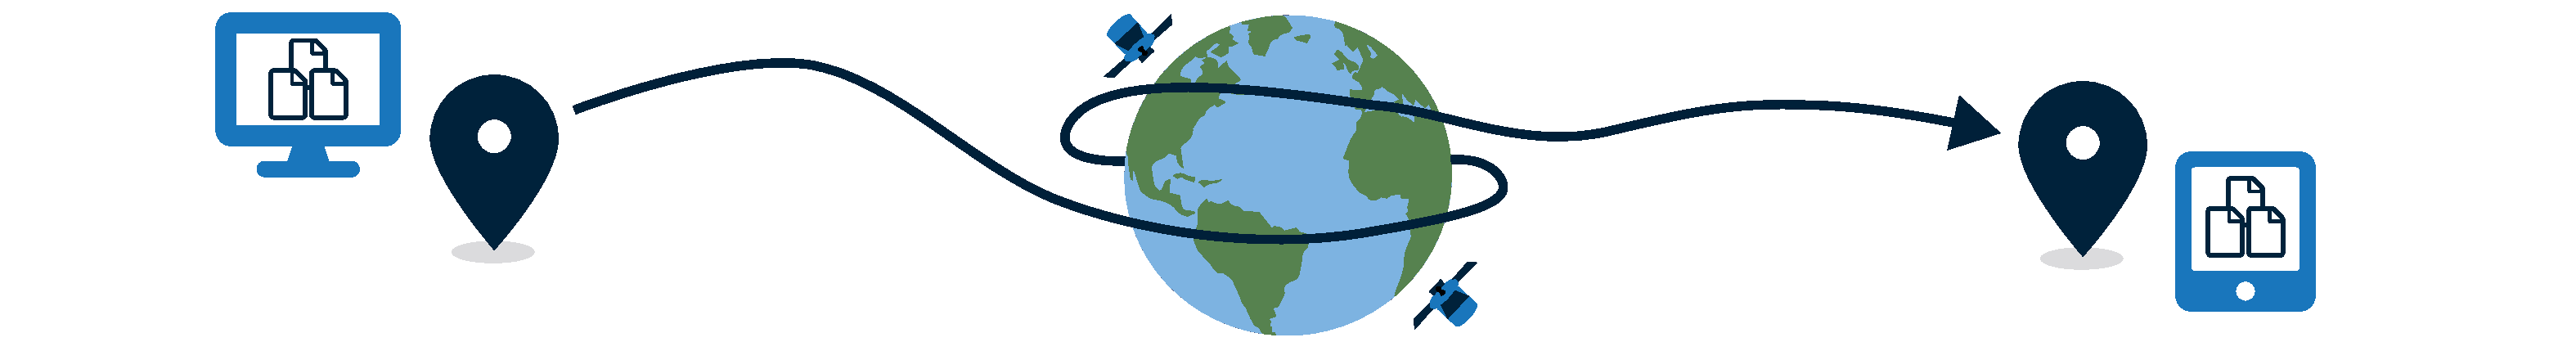
\includegraphics{figures/ch1-earth.pdf}}
    \label{fig:stopsign}
    \vspace{-4mm}
\end{figure}

Sifting through such large volumes of information online to find the elusive and proverbial \emph{needle in the haystack} has been an area of active research and development over a number of decades. Since the early 1990's, the~\gls{acr:www} has emerged as the dominant means of publishing information online over the Internet, replacing obsolete technologies such as the \emph{Gopher} protocol.\footnote{Gopher was designed primarily with a menu-driven interface in mind (i.e. selecting options from a series of choices). The Gopher ecosystem provided the foundations for the~\gls{acr:http} protocol, which the~\gls{acr:www} today utilises.}. As the amount of information available on the~\gls{acr:www} grew\footnote{According to \url{http://www.internetlivestats.com/total-number-of-websites/}, September 2014 saw the point at which 1 billion unique websites were present on the~\gls{acr:www}.\urlaccessed{2018-05-21}}, so too did the paradigms that were employed by those wishing to seek information on it.

Over the course of the \emph{noughties}, the approach demonstrated by \emph{information seekers} for finding information online changed from the concept of \emph{surfing} a particular domain by following a series of set~\glspl{glos:hyperlink} within documents, to explicitly \blueboxbold{searching} the ever increasing universe of documents available at their disposal (refer to Figure~\ref{fig:ch1-surfing}).\footnote{Indeed,~\cite{mcbryan1994taming_tools} considered a search engine as a means of \emph{taming} the considerable number of documents online.} This is not to say that surfing no longer occurs; procrastinators (the author included...) might find solace by surfing the myriad of content available on \emph{Reddit,} billed as the \emph{``front page of the Internet''}\footnote{\url{https://www.reddit.com}\urlaccessed{2018-05-21}}. However, for a task where an individual has a specific \emph{information need,} searching become by far the most dominant paradigm for seeking required information. As such, the development of effective \emph{search engines} has been of paramount importance, with the development of search engines seen as the \emph{raison d'\^{e}tre} of the study of~\gls{acr:ir}.

\begin{figure}[t!]
    \centering
    \resizebox{1\hsize}{!}{
    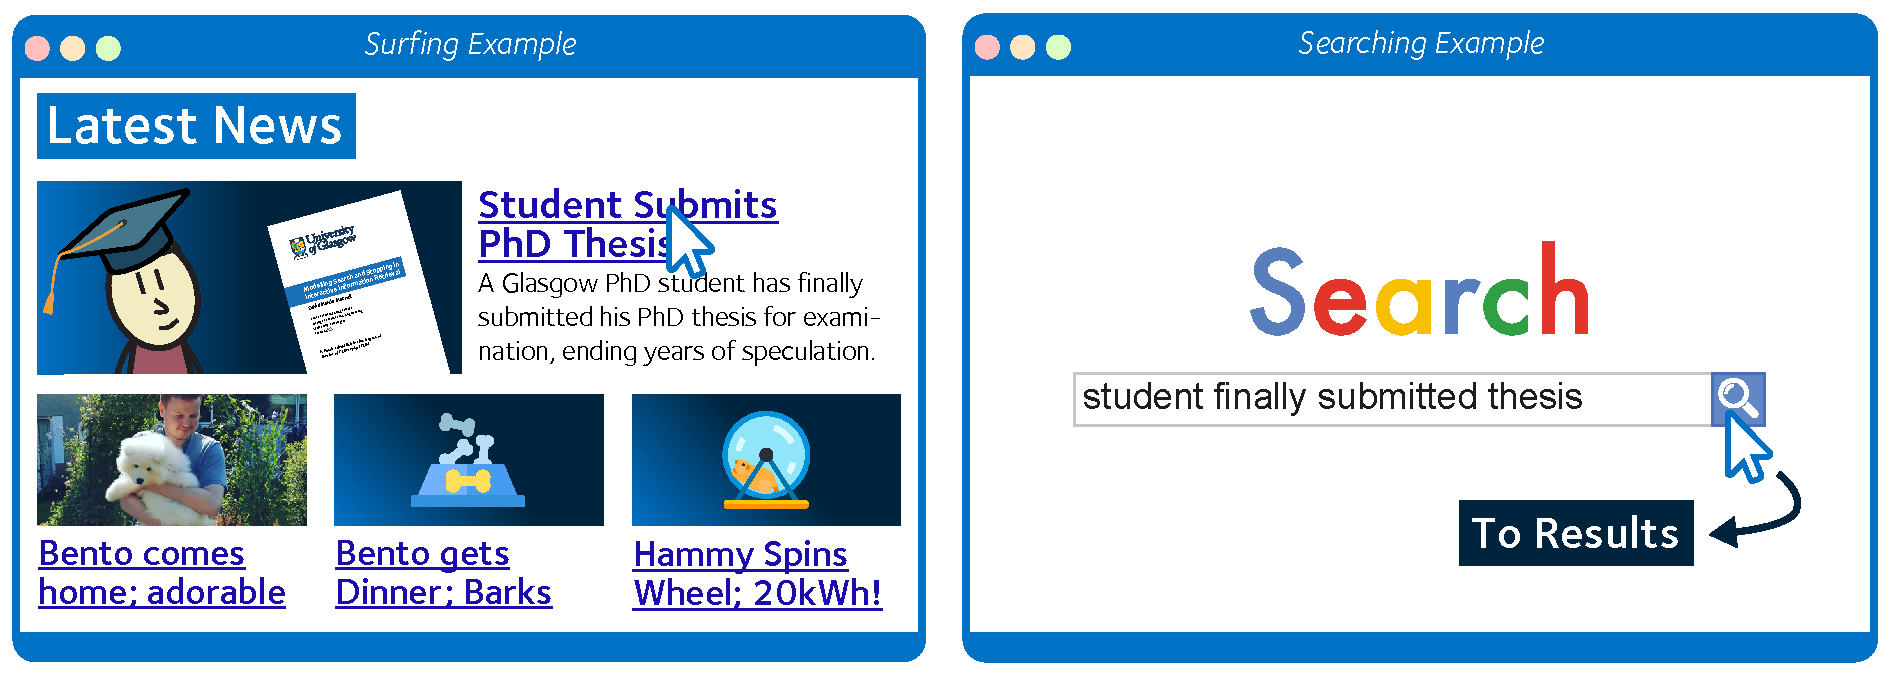
\includegraphics{figures/ch1-surfing.pdf}}
    \caption[Surfing vs. Searching]{The paradigms of surfing and searching. On the left, a seeker will navigate through a series of documents via~\glspl{glos:hyperlink} (perhaps without a specific \emph{information need} in mind), while a searcher (right) will issue a \emph{query} articulating their information need, relying on an underlying \emph{search engine} to \emph{retrieve} documents that it thinks will assist the seeker.}
    \label{fig:ch1-surfing}
\end{figure}

\begin{quote}
    \emph{``...but perhaps the key technology that took the web from a useful supplement of current information practice to become the default communication medium is search.''}
    \attrib{\cite{wilson2010keyword_search}}
\end{quote}

Contemporary search engines such as \emph{Google} and \emph{Bing} are considered to offer an effective means of finding the proverbial needle in the haystack~\citep{wilson2010keyword_search}, where near perfect accuracy is regularly attained for popular \emph{queries}~\citep{vaughan2004new_measurements}. These search engines, along with the many others in existence today under a variety of different contexts\footnote{Google and Bing may be the most popular search engines for \emph{general web queries,} but other contexts can include patent search, enterprise search and multimedia search, as examples.}, are the product of the collective work undertaken in the field of~\gls{acr:ir} -- from early research in the 1970's~\citep{cleverdon1962cranfield_experiments,rijsbergen1979ir}; to the development of various \emph{retrieval models}~\citep{robertson2009probabilistic_models}; to the setting up of \emph{evaluation forums}~\citep{harman1993trec1}; to the development of the \emph{large-scale search engines} (or \emph{retrieval systems}) that are commonplace today~\citep{baezayates1999modern_ir, wang2010language_models}.

The work that the field of~\gls{acr:ir} collectively undertakes is all done in the interests of making it easier for potential users of search engines to satisfy their underlying \emph{information need}. Armed with a preexisting knowledge of the world, an individual will develop an information need from a perceived problem -- either from a knowledge gap, an internal consistency, or a conflict of evidence. This state has been referred to as the \emph{anomalous state of knowledge}~\citep{belkin1980ask}. A searcher then formulates a \emph{query} -- an expression of what they are looking for~\citep{borlund2003iir_model}, typically consisting of a number of different terms -- before being presented with a potentially relevant set of documents. From this set of documents, an individual can then begin the process of examining them for relevance. A number of complex interactions take place between an individual seeking information and the search engine that is being utilised~\citep{ingwersen2005theturn}. This process, where the searcher engages in \emph{dialogue} with the search system, is considered the study of~\glsfirst{acr:iir}~\citep{borlund2003iir_model}. As such, work has been undertaken that attempts to help us better understand these complex interactions, and potentially assist in making the search process a more seamless experience.

\section{Motivation and Context}\label{sec:intro:motivation}
Central to much of the work undertaken in the field of~\gls{acr:ir} over the past 50 years is the so-called \emph{Cranfield paradigm}, a term denoting a standardised approach for the \emph{evaluation} of~\gls{acr:ir} systems. The Cranfield paradigm descends directly from \emph{Cranfield II}~\citep{aslib1966factors}, a set of experiments designed to evaluate the efficiency of \emph{indexing systems}\footnote{The process of indexing, as discussed later in Section~\ref{sec:ir_background:basics:indexing}, involves turning a number of source documents into a form of data structure that can be traversed, or \emph{searched,} in a quick and efficient manner.}. At the time, searching for information on computer systems was achieved through the issuance of queries to a \emph{boolean retrieval system} (refer to Section~\ref{sec:ir_background:basics:models:boolean}), with terms matched against a small set of manually indexed documents~\citep{harman2010cranfield}. Results were compared against a set of \emph{a priori} \emph{relevance judgements} for each of the documents, as judged by humans, allowing one to then ascertain the performance of a given retrieval system.
%We discuss this high-level approach in Section~\ref{sec:ir_background:basics:cranfield}.

While the basic principles of the Cranfield paradigm have remained in place since it was established in the 1960's, components of the approach have evolved over the years to cater for the ever increasing complexity of the tasks at hand~\citep{harman2010cranfield}. Indeed, the approach is still widely used in evaluation forums, such as the~\gls{acr:nist} sponsored~\gls{acr:trec} -- the first of which was held in 1993~\citep{harman1993trec1}. Indeed, many of the relevance judgements and \emph{topics} (i.e. information needs) provided as part of \emph{\gls{acr:trec} Tracks} over a number of years are used as ground truths throughout the work discussed in this thesis.

This approach however can be argued to remain simplistic in terms of consideration of the complex user interactions that take place during the search process~\citep{borlund2000evaluation_iir,ingwersen2005theturn}. In other words, the Cranfield paradigm broadly fails to consider the complexities of the~\gls{acr:iir} process, where, for example, searchers can issue multiple queries during the course of a search session, and adapt their interactions based upon the perceived quality of the presented ranked list of results for each associated query~\citep{moffat2013users_versus_models}. Selecting good terms to use within a query is difficult yet important~\citep{efthimiadis2000query_expansion}; as such, the initial query posed in a search session often acts as an entry to the search system, followed by phases of browsing and query reformulations~\citep{marchionini1993information_seeking}.

Searchers also will typically abide by the principle of least effort, whereby they strive to minimise the probable average rate of work expenditure over time~\citep{zipf1949behaviour}. Cranfield makes a series of assumptions, namely that that a user will: \emph{(i)} issue a single query; \emph{(ii)} examine documents to a great depth (typically $1,000$ documents); and \emph{(iii)} consider all documents to be relevant. This is largely unrealistic, and numerous researchers have proposed alternatives to the Cranfield paradigm --~\cite{borlund2003iir_model}, for example.

Considering alternatives to the Cranfield paradigm,~\cite{keskustalo2008user_simulation} categorised~\gls{acr:iir} research into four different approaches that allow for the consideration of the complex interactions that take place between a human and the search engine being used. The four approaches, as illustrated in Figure~\ref{fig:ch1-options}, can themselves be divided into two categories. The first category considers approaches that utilise \blueboxbold{real-world searchers}, namely:

\begin{itemize}
    \item[]{\blueboxbold{1} the \blueboxbold{observation of real-world searchers} in real world scenarios (e.g. general web search), through the use of \emph{interaction logs;} and}
    \item[]{\blueboxbold{2} the observation of \blueboxbold{real-world searchers undertaking simulated work tasks} in a lab-based environment (i.e. a \emph{user study}).}
\end{itemize}

The final two options \emph{do not explicitly} consider real-world searchers, but rather aim to mimic their behaviours. These approaches are:

\begin{itemize}
    \item[]{\blueboxbold{3} performing \blueboxbold{simulations of interaction} in a lab-based environment, \emph{sans} real-world searchers; and of course}
    \item[]{\blueboxbold{4} the undertaking of \blueboxbold{traditional, Cranfield style lab-based experimentation}.}
\end{itemize}

\begin{figure}[t!]
    \centering
    \resizebox{1\hsize}{!}{
    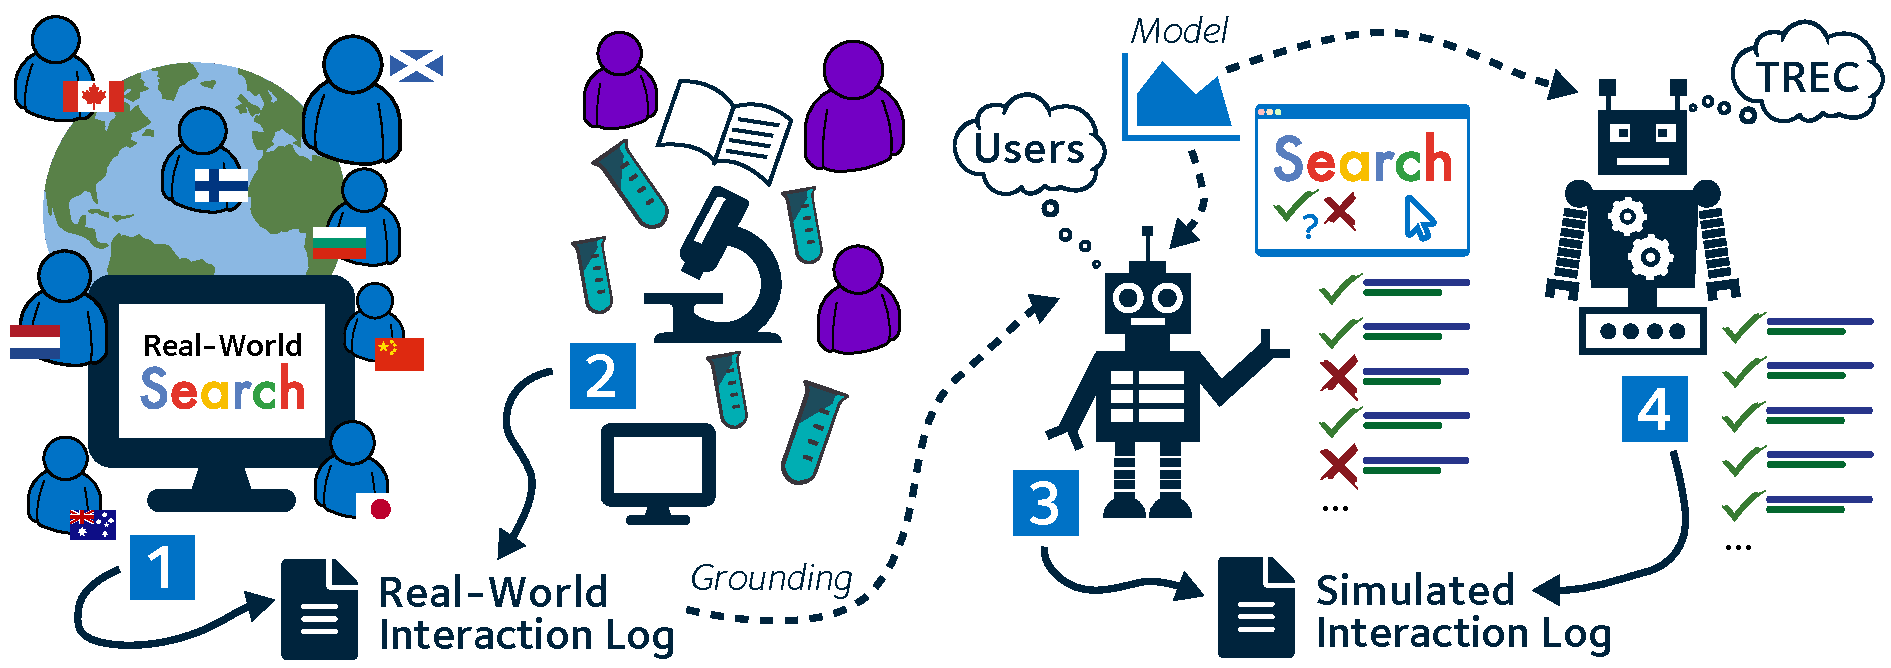
\includegraphics{figures/ch1-options.pdf}}
    \caption[Approaches to~\gls{acr:iir} research]{The four approaches for~\gls{acr:iir} research, as outlined by~\cite{keskustalo2008user_simulation}. Detailed in Section~\ref{sec:intro:motivation}, approaches \blueboxbold{1} \emph{(real-world)} and \blueboxbold{2} \emph{(user studies)} consider log data from real-world searchers, with options \blueboxbold{3} \emph{(simulations of interaction)} and \blueboxbold{4} \emph{(traditional experimentation)} considering log data as generated from \emph{simulations.} Note the \emph{grounding} (dashed line) of log data from either approach \blueboxbold{1} or \blueboxbold{2} to complement approach \blueboxbold{3} (refer to Section~\ref{sec:intro:simulation}).\vspace*{10mm}}
    \label{fig:ch1-options}
\end{figure}

Obtaining interaction data from studies utilising real-world users undertaking search tasks (categories \blueboxbold{1} and \blueboxbold{2}) will of course always be the preferred option. There can never be a better substitute than examining the real thing. However, there are pitfalls with both approaches that must be considered, primarily in terms of \emph{availability} and \emph{cost}. Obtaining data for studies conducted in category \blueboxbold{1} is difficult if the researchers do not work for an organisation offering a large-scale search engine, such as \emph{Google} or \emph{Microsoft.} Working within an academic setting for example may greatly restrict what data can be obtained. Indeed, working with real-world interaction data also leads to major ethical and privacy concerns~\citep{korolova2009aol_query_log_privacy}. The release of the \emph{AOL Query Log} (and subsequent fallout) in August 2006 is testament to that, although this has not stopped researchers from utilising the data in their work (refer to~\cite{brenes2009aol_query_log} for such an example).

This will leave many researchers with category \blueboxbold{2} -- especially those in a non-industrial setting. While this approach also leads to the capturing of real-world interaction data, pitfalls of this approach primarily are the significant costs involved in such an approach -- both financially and in terms of time. Considerations must also be placed into study design to mitigate potential biases. In recent years however, the concept of \emph{crowdsourcing} may alleviate some of these concerns, and open up a potential study to a larger potential audience. A recent study has shown that using crowdsourcing to capture interaction data is no worse than a carefully controlled lab-based user study~\citep{zuccon2013crowdsourcing_comparisons}, although quality control measures must be taken.

While categories \blueboxbold{1} and \blueboxbold{2} provide real-world interaction data, options \blueboxbold{3} and \blueboxbold{4} do not. Such approaches however, if executed correctly, can potentially lead to insights that would not otherwise be possible when involving real-world users. As an example, covering an extensive set of test cases with real-world searchers may simply not be possible~\citep{keskustalo2008user_simulation} -- perhaps due to financial constraints, or a lack of suitable subjects. Category \blueboxbold{4} can be considered as a means of conducting \emph{traditional, TREC-style}~\gls{acr:ir} lab experimentation that is, as previously mentioned, largely na\"{i}ve of the user's complex interactions. This leaves category \blueboxbold{3} as a means of conducting and evaluating user-sided experimentation without the explicit need for real-world users to be present. \blueboxbold{Simulation} is used as a means to conducting such experiments.

\subsection{Considering Simulation}\label{sec:intro:simulation}
Simulation is defined as the \emph{imitation of the operation of a real-world process or system over time}~\citep{banks1996discrete}. Such an approach allows one to gain insight into the functioning of some real-world phenomenon. Simulation has been used in a wide range of areas, including, for example, examining physical processes~\citep{haessig1991physics_modelling}, psychology~\citep{hastie1988human_memory_simulation}, road traffic~\citep{mahmud2016traffic_modelling_electric} and training for various activities, such as piloting an aeroplane~\citep{sparko2010flight_simulators}. Central to contemporary uses of simulation is the idea of \emph{computerised simulation}~\citep{heermann1990computer_simulation}. Thanks to ever increasing computational power in~\glspl{acr:cpu} and~\glspl{acr:gpu} available for such tasks, such as the simulation of racing cars for the purposes of driver development, as shown in Figure~\ref{fig:ch1-mclaren}. With computer simulation, a real-world object can be imitated with varying degrees of realism. Alternatively, individual components that comprise a larger system can be examined and simulated in isolation, allowing researchers to obtain a more detailed understanding of how individual components react to changes in their environment. As such, simulation can provide a rapid means of exploring aspects of a real-world phenomenon, all at a low cost -- all the while permitting repeatable, and therefore reproducible, results~\citep{maxwell2016agents}.

\begin{figure}[t!]
    \centering
    \resizebox{1\hsize}{!}{
    \includegraphics{figures/ch1-mclaren.jpg}}
    \caption[Racing Simulator Example]{An example of a \emph{video game simulation}, \emph{Assetto Corsa}. In this illustration is a model of the \emph{McLaren-Mercedes MP4/13} race car (complete with terrible gear ratios), driving around the \emph{Autodromo Enzo e Dino Ferrari} circuit in northeastern Italy. In the past ten years, increases in~\gls{acr:cpu} and~\gls{acr:gpu} performance has enabled the development of increasingly complex (and \emph{more realistic}) video game simulations, which, for example, are now used in the training of racing drivers.}
    \label{fig:ch1-mclaren}
\end{figure}

One of the key components of any simulation -- regardless of whether it is executed on a computer or not -- is that of an underlying \emph{model} of the real-world phenomenon being simulated~\citep{tocher1963art_of_simulation}. This model defines the various stages, rules and other descriptive components of the phenomenon that simulations must consider. These rules are often high level, and as such, a number of \emph{assumptions} are made~\citep{tocher1963art_of_simulation}. For example, the~\gls{acr:trec} model of search (as detailed in Section~\ref{sec:stopping_background:models}) assumes that a single query is issued by a searcher within a search session, and searchers examine to great depths per query. These assumptions should be made in the face of supporting evidence; evidence in~\gls{acr:iir} studies strongly suggests that searchers do not follow this rigid approach, but rather adapt their behaviour based upon cues that are presented to them.

Why though, use simulation when other alternatives to modelling the search process are available? Alternatives include some form of closed-form system, such as a series of linear equations to describe the complex interactions that take place. However, according to~\cite{fishwick1995simulation}, this approach is not flexible enough, and a number of reasons are linked as to why simulation is essential in complex, dynamic systems:

\begin{itemize}
    \item{the model is very complex, with many variables and interacting components;}
    \item{the underlying variables and relationships are non-linear;}
    \item{the underlying models contains random variates; and}
    \item{the model output is to be visual, as in a three-dimensional computer animation.}
\end{itemize}

In the context of~\gls{acr:iir}, the first three reasons can be considered as acceptable reasons for why simulation is an advantageous methodology to pursue. For example, many state-of-the-art~\gls{acr:iir} models consider a stochastic component when determining the relevancy of a document to a particular information need (or~\gls{acr:trec} topic).

Simulation provides a means of using a uniform model execution technique that can be used to solve a large variety of systems, without resorting to a \emph{``bag of tricks'',} where one must choose special purpose and sometimes arcane solutions to avoid simulation~\citep{fishwick1995simulation}. Simulation provides the freedom and flexibility to permit the implementation of a model that better represents the real-world phenomenon that is being considered. In contrast, with a more closed-form approach, the underlying model that is created is often twisted and altered to suite the closed-form approach, rather than to actually represent the real-world system. This leads to a larger gap between the model and reality, and as such leads to a greater number of assumptions within the model than what would otherwise be required. In other words, the technique used to develop the model constrains just how realistic is can be. Simulation provides the freedom and flexibility to reduce assumptions that may otherwise be included.

As a means of testing better and more flexible models of search, simulation has been extensively used within~\gls{acr:ir}. While we provide an overview of simulation of~\gls{acr:ir} in Section~\ref{sec:ir_background:user:simulation}, one such area that has been studied is \emph{simulated interaction,} where one attempts to mimic the behaviours that a searcher exerts when interacting with a search engine -- and is exactly what we consider in this thesis. While this encapsulates category \blueboxbold{3} of the four categories outlined by~\cite{keskustalo2008user_simulation}, we also argue that in order to run simulations of interaction \emph{`correctly',} they must be \emph{grounded} using real-world observations, which in turn means that the assumptions can be considered to be credible abstractions of the real-world phenomenon. As such, this necessitates access to data obtained through either categories \blueboxbold{1} or \blueboxbold{2} -- or, in other words, data from \emph{real-world searchers.} Without access to a large-scale search engine for this research, this leaves category \blueboxbold{2} as a means for acquiring such data, and provides an explanation between the linking of the real-world interaction log, and simulated users (via the dashed line) in Figure~\ref{fig:ch1-options} on page~\pageref{fig:ch1-options}.

\noindent
\blueboxbold{In a Nutshell – Simulation and this Thesis}
Given all of the above, this thesis proposes a more advanced, realistic model of the search process. In line with the suggestions outlined in the work by~\cite{keskustalo2008user_simulation}, simulations of interaction are trialled (category \blueboxbold{3}), with the underlying components of the model \emph{grounded} using interaction data extracted from two different user studies, also conducted as part of this thesis. One particularly important phenomenon that has been largely overlooked in the~\gls{acr:iir} literature is that of a searcher's \blueboxbold{stopping behaviour} (e.g. \emph{given this list of ranked results, how far down the list should I go before I stop?}). In the next section, we provide a brief introduction on why stopping behaviour is important, before considering this thesis' research statement.

\subsection{Considering Stopping Behaviours}\label{sec:intro:stopping}
\begin{wrapfigure}[7]{r}{0.45\textwidth}
    \begin{center}
    \vspace*{-10mm}
    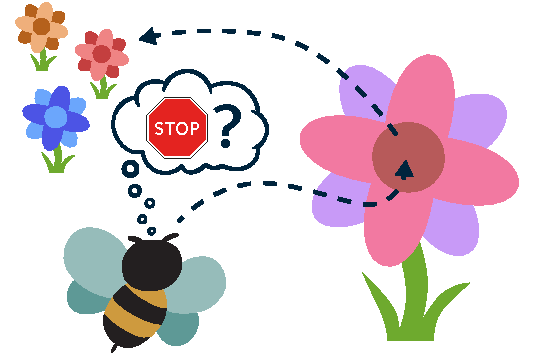
\includegraphics[width=1\textwidth]{figures/ch1-bee.pdf}
    \end{center}
    \vspace*{-4mm}
    \label{fig:bee}
\end{wrapfigure}

With any activity that a creature makes, there has to come a time when it makes a decision to \emph{stop} what it is doing. A honeybee, when collecting pollen on a flowerhead, will eventually stop collecting and fly away to another flower. An exhausted PhD student, when writing his or her thesis, will eventually stop writing for the night once he or she has become too tired -- something the author knows only all too well. Similarly, when applied to the context of search, an individual will also make a decision to eventually stop examining content. These examples demonstrate that knowing when to stop is a fundamental aspect of animal -- and by definition, human -- thinking and behaviour.

But given this, what actually makes us decide when to stop doing something? Obviously, different \emph{external factors} can influence this decision, such as finding no more pollen on a flowerhead, or time pressure that is exerted upon us. Moreover,~\citep{nickles1995judgment} argues that \emph{knowing when to stop} is largely determined by a series of \emph{internally defined, stopping criteria} that the decision maker employs. This makes stopping a phenomenon that is incredibly difficult to model effectively. We discuss this in more detail in Section~\ref{chap:stopping_background:why}.

Given the fact that internal factors are a major drive to determining when to stop, studies have largely been unable to quantify \emph{why} searchers stop, other than what they find gives them the feeling that it is \emph{``good enough''}~\citep{zach2005enough_is_enough}. Researchers have however attempted to create a series of \emph{reasoning} and \emph{judgement} based \blueboxbold{stopping heuristics} that attempt to formally define when a searcher should stop. It is these stopping heuristics that we will primarily consider in this thesis. In conjunction with an updated user model of search, these heuristics can then be integrated into the model, allowing us to determine whether they offer better or worse approximations of actual searcher stopping behaviours.

Examining stopping behaviour during search is important because it considers the judgements of a searcher as part of their interactions. For example, it would be prudent of a searcher examining a list of results that are mostly considered to be non-relevant to a given information need to stop early, and thus save time and effort. In other words, a good stopping heuristic allows a searcher to become \emph{more efficient.} This can be achieved in a number of different places -- or \blueboxbold{stopping decision points} -- during search, such as the depth to which a searcher will examine a list of results.

\section{Overarching Research Questions}\label{sec:intro:rqs}
From the introductory explanations of the problem space above, we can now formulate the four main overarching, high level research questions -- denoted as \blueboxbold{HL-RQ} -- that the work in this thesis addresses. Our first research question considers the concept of user modelling, and how, with an emphasis of examining stopping decision points, we can improve the current model to better reflect actual searcher behaviours.

\begin{itemize}
    \item[]{\blueboxbold{HL-RQ1} How can we improve the current state-of-the-art searcher model to incorporate different points where individuals subscribing to such a model can stop?}
\end{itemize}

As previously stated, being able to improve the current state-of-the-art from a stopping perspective should allow those subscribing to such a model to become more efficient at how they search. Closely related to this advancement in user modelling is the consideration of the various stopping heuristics, as briefly outlined in Section~\ref{sec:intro:stopping}.

\begin{itemize}
    \item[]{\blueboxbold{HL-RQ2} Given the stopping heuristics defined in the literature, how can we encode these heuristics into a series of operationalised, programmable \blueboxbold{stopping strategies} that can be subsequently evaluated?}
\end{itemize}

The heuristics that we detail later in Section~\ref{sec:stopping_background:heuristics} are high level in nature, and no not provide an explanation as to how they can be \emph{operationalised} within a wider system. The challenge that must be addressed in order to answer this question will be how we can operationalise these heuristics within a wider, common framework.

Our final two overarching research questions can be considered similar in nature, and are numbered as such. With a more realistic model of the search process defined by addressing \blueboxbold{HL-RQ1} and a series of stopping strategies defined by addressing \blueboxbold{HL-RQ2}, how well do the combinations of an improved model and different stopping strategies perform?

\begin{itemize}
    \item[]{\blueboxbold{HL-RQ3a} Given these operationalised stopping strategies, how well do simulated searchers using these strategies perform?}
    \item[]{\blueboxbold{HL-RQ3b} How closely do the operationalised stopping strategies compare to the stopping behaviours of real-world searchers?}
\end{itemize}

With the flexibility provided by the approach, simulation is an ideal mechanism for achieving a means to address these two research questions. These questions are of course very broad in nature -- as should be expected for overarching questions -- and it is simply not possible to evaluate them in every conceivable search context. As we discuss in the following section, we will examine these questions in several different contexts which are likely to impact upon the stopping behaviours of searchers.

\section{Thesis Contributions}\label{sec:intro:contribs}
From our four overarching research questions defined above, we identify four major contributions offered by the work presented in this thesis. Listed and detailed below, we consider primary contributions from conceptual, theoretical and empirical standpoints. We also consider the general methodology that we utilise throughout the work in this thesis.

\noindent
\blueboxbold{Conceptual Model}
Our first contribution is that of a searcher model. Taking the current state-of-the-art, we propose an updated, high-level model of the search process. We call this model the \blueboxbold{\gls{acr:csm}}, and this provides us with a solution for addressing \blueboxbold{HL-RQ1}. Outlined in Section~\ref{sec:csm:csm}, the conceptual~\gls{acr:csm} outlines a series of different activities and decision points that searchers undertake throughout the search process, and establishes a flow of interaction based upon established models. Within the~\gls{acr:csm} are a number of innovations, central to the work in this being a new stopping decision point. Combined together, these improvements allow us to ascertain a better understanding of the search process, and the complex interactions between a searcher and search system that take place. Being a conceptual model, we can take the~\gls{acr:csm} and instantiate it in a number of different ways. For example, the stopping decision points (i.e. \emph{should I continue examining this set of results?}) must be instantiated -- and for this, our second contribution provides a solution to this problem.

\noindent
\blueboxbold{Theoretical Examination}
As briefly outlined in Section~\ref{sec:intro:stopping}, there are a range of different stopping heuristics that have been defined in the literature -- some directly applicable to search, some defined in other branches of science (such as ecology, for example). The second major contribution of this thesis is the development of a series of operationalised, programmable stopping strategies that can be subsequently implemented as a stopping decision point of the~\gls{acr:csm}, defined above. These are delivered within a common framework. These operationalised stopping strategies provide a solution to our second overarching research question, \blueboxbold{HL-RQ2}.

\noindent
\blueboxbold{Empirical Studies}
As discussed in Section~\ref{sec:intro:rqs}, the~\gls{acr:csm} and the various stopping strategies that we operationalise need to be evaluated, such that we can then subsequently address \blueboxbold{HL-RQ3a} and \blueboxbold{HL-RQ3b}. To do this, the third major contribution of this thesis is empirical. We conduct two user studies, choosing to examine different factors which are likely to affect stopping behaviours. These factors are:

\begin{itemize}
    \item{varying snippet length (and subsequently snippet quality);}
    \item{varying task goals -- from time-limited to \emph{find $x$ relevant items}; and}
    \item{varying task type, considering \emph{ad-hoc topic retrieval} and \emph{diversifying results.}}
\end{itemize}

These studies are part of the \blueboxbold{general methodology} that we utilise. After the user studies have been completed and stopping behaviours investigated empirically, we then use the data from these studies to ground a series of simulations, as discussed in Section~\ref{sec:intro:simulation}. This improves the credibility of the simulations, which are then examined, and allow us to: address which stopping strategies (under a certain context); offer \blueboxbold{HL-RQ3a} the best overall performance; and \blueboxbold{HL-RQ3b} closest approximations to actual searcher behaviours. Simulations are conducted entirely using a custom built simulation framework, \blueboxbold{SimIIR}.

\section{Thesis Statement}
Given the above, the statement of this thesis is that by considering additional stopping decision points within a model of the interactions between a searcher and a search system, one can run simulations of interaction that offer a greater degree of realism of searcher behaviour. Thus, this leads to us acquiring a more comprehensive understanding of the complex interactions that take place.

%Thus, one should be able to deduce an optimal \emph{stopping strategy} yielding high performance, and a better approximation of the actual behaviours exhibited by real-world searchers than currently employed models.

In particular, incorporating such stopping decision points within a model of the search process will allow a simulated user abiding by it a greater degree of flexibility in the search strategy that they employ. For example, a searcher will be able to abandon a set of results that is judged to be of low relevance to a given information need. This will allow abandonment comparatively earlier than a set of results that are perceived to be of higher quality. In addition, these stopping decision points can be instantiated by operationalising a series of different stopping heuristics that are \emph{believed}~\citep{maxwell2015stopping_strategies} to encapsulate the stopping behaviours exhibited by real-world searchers. By taking this knowledge forward, we can then ground these simulations of interaction over a variety of different search contexts with differing goals, examining how the stopping behaviours of searchers varies under each context. Through simulation, we can then deduce what particular heuristic(s) offer the best performance and best approximations to actual searcher behaviours.

\section{Origins of the Material}
Material presented in this thesis has appeared in several conference papers throughout the duration of the author's PhD programme, from October 2013 to June 2018. All are listed in the front matter of this thesis in chronological order. In this section, we provide narrative, explaining how the developments in the listed publications led to the contributions of this thesis, listed above. Work can be considered over three main strands:

\begin{itemize}
    \item{the development of the conceptual and theoretical contributions to this work;}
    \item{the development of the SimIIR framework; and}
    \item{a series of empirical studies.}
\end{itemize}

\noindent
\blueboxbold{Conceptual and Theoretical}
Work on the~\gls{acr:csm} has been undertaken over a number of years. A number of iterations of the~\gls{acr:csm} were presented in various publications. However, in order to simplify the work reported in this thesis, we consider only the latest iteration. The first version of the~\gls{acr:csm}, essentially analogous to the prior models of search outlined in Section~\ref{sec:stopping_background:models:conceptual:simple}, were outlined and used in simulated analyses, as reported in two publications.

\begin{itemize}
    \item{\bibentry{maxwell2015initial_stopping}}
    \item{\bibentry{maxwell2015stopping_strategies}}
\end{itemize}

These publications are notable for also including a number of operationalised stopping strategies, providing the foundations for the second major contribution of this thesis. The stopping strategies defined in these publications were used in subsequent publications. Further developments to the~\gls{acr:csm} were found in a subsequent publication which experimented with the notion of \emph{intelligent search agents}.

\begin{itemize}
    \item{\bibentry{maxwell2016agents}}
\end{itemize}

The final development of the~\gls{acr:csm} led to the inclusion of a third stopping decision point, complete with a large-scale simulated analysis. This led to the finding that the inclusion of the new decision point within the~\gls{acr:csm} led to improvements in overall search performance, and approximations of actual searcher behaviours.

\begin{itemize}
    \item{\bibentry{maxwell2018serp}}
\end{itemize}

\noindent
\blueboxbold{SimIIR Framework}
One of the major pieces of scientific apparatus utilised throughout all of the aforementioned studies is the SimIIR framework, touched upon in Section~\ref{sec:intro:contribs}. While we do not explicitly discuss the framework in great depth in this thesis, but rather focus on how we implemented the different components, conducting the simulated analyses would not have been possible without it. A publication demonstrating the framework and the various components that could be instantiated was published.

\begin{itemize}
    \item{\bibentry{maxwell2016simiir}}
\end{itemize}

\noindent
\blueboxbold{Empirical Studies}
The general methodology that we employ for the third major contribution of this thesis has been introduced and refined in the publications listed previously. In addition to this, a basic description of the methodology is provided in a Doctoral Consortium paper that the author presented at the first \emph{ACM Conference on Human Information Interaction and Retrieval (CHIIR)} in Chapel Hill, NC, USA.

\begin{itemize}
    \item{\bibentry{maxwell2016dc}}
\end{itemize}

The results of two studies were also published, and are of direct relevance to the work detailed later in this thesis.

\begin{itemize}
    \item{\bibentry{maxwell2014temporal_delays}}
    \item{\bibentry{maxwell2017snippets}}
\end{itemize}

These studies provide the grounding for simulated analyses that we also consider later in this thesis. The data extracted from these user studies provides credibility to our simulations, through the extraction of aspects such as interaction costs and probabilities.

\section{Remaining Thesis Outline}
Now that our motivation, research questions and thesis contributions have been outlined, this section provides a brief summary of the remaining chapters of the thesis. Split into four parts, the chapters are summarised below.

\noindent
\darkblueboxbold{Part I}
The remainder of Part I concerns prior work that has been undertaken in the fields of~\gls{acr:ir} and~\gls{acr:iir}. Two chapters discuss the basics of~\gls{acr:ir} and~\gls{acr:iir}, before we begin to examine prior work that considers search and stopping.

\begin{itemize}
    \item[]{\blueboxbold{Chapter 2}} Beginning on page~\pageref{chap:ir_background}, this chapter provides an overview of the key concepts of the fields of~\gls{acr:ir} and~\gls{acr:iir}. In particular, we focus on basic~\gls{acr:ir} concepts such as the indexing and retrieval processes (including retrieval models), before moving towards a more user-centric examination of various evaluation measures that are commonly deployed in~\gls{acr:iir} research.
    
    \item[]{\blueboxbold{Chapter 3}} We then consider work that has been undertaken in relation to stopping behaviours. In this chapter, we focus on the development of various stopping heuristics, examine previous studies that have examined searcher stopping behaviours, examine key theoretical models of search that provide explanations for when individuals stop, and finally discuss prior models of search -- focusing particularly on the components that consider stopping behaviours. 
\end{itemize}

\noindent
\darkblueboxbold{Part II} Beginning on page~\pageref{part:stopping}, Part II begins to consider the conceptual and theoretical contributions of this thesis, including a discussion of the~\gls{acr:csm}. We also in this part of the thesis provide an outline of the general methodology that is extensively utilised in Part III.

\begin{itemize}
    \item[]{\blueboxbold{Chapter 4} This chapter introduces the~\gls{acr:csm}, discussing the advancements the conceptual model provides over the current state-of-the-art. We discuss the key stopping decision points provided by the~\gls{acr:csm} that are central to this thesis, before discussing the assumptions of the model.}
    
    \item[]{\blueboxbold{Chapter 5} In this chapter, we introduce and discuss the various stopping strategies that we operationalise as part of the contributions of this thesis. Each of the different stopping strategies are discussed in depth, complete with examples of each. The chosen stopping strategies are linked back to their source stopping heuristics, which are detailed in Chapter~\ref{chap:stopping_background}.}
    
    \item[]{\blueboxbold{Chapter 6} The third chapter of this part outlines our general methodology, detailing the high-level structure of the scientific method used in the empirical work discussed in Part III. We also provide in-depth discussion of common approaches that were followed across all subsequent chapters, providing a neat overview of the work that was undertaken.}
\end{itemize}

\noindent
\darkblueboxbold{Part III}
The third part of this thesis considers the empirical contributions that are made. In this part, we discuss the user studies that were undertaken, as well as a number of simulated analyses that allow us to address research questions \blueboxbold{HL-RQ3a} and \blueboxbold{HL-RQ3b}.

\begin{itemize}
    \item[]{\blueboxbold{Chapter 7} This first empirical chapter considers how a searcher's behaviour varies when the length (and subsequently quality) of snippets is varied. We provide a discussion of a user study that examined this phenomenon, before summarising the findings of a simulated analyses that was conducted in order to determine what stopping strategies offered the best performance and approximations under this context.}
    \item[]{\blueboxbold{Chapter 8} A similar approach to the chapter above is followed here, with a variation on the user study discussed and subsequently simulated. In this chapter, we examine how a searcher's stopping behaviour varies when subjected to different constraints and task goals, considering time limits, \emph{find $x$} and diversified and non-diversified tasks.}
    \item[]{\blueboxbold{Chapter 9} This final contributory chapter of the thesis considers the new stopping decision point that is provided by the~\gls{acr:csm}. We empirically test the~\gls{acr:csm}, allowing us to determine whether the inclusion of the new stopping decision point discussed in Chapter~\ref{chap:csm} provides improvements in overall performance and approximations of actual searcher behaviours. Conducted via simulation, we utilise data from user studies discussed in prior chapters to ground these reported simulations.}
\end{itemize}

\noindent
\darkblueboxbold{Part IV} Consists of a single chapter, \blueboxbold{Chapter 10}. The concluding chapter of this thesis provides a summary of the work that was undertaken, and the results that were subsequently found. We then consider the results and discuss what they mean in terms of directions for future work.





% From the introductory explanations of the problem space above, we can now enumerate the three main contributions that this thesis provides to the community.
%
%
% This thesis offers four main contributions to the research community, revolving around the concepts of user modelling and stopping behaviours during search.
%
% \begin{itemize}
%     \item[\blueboxbold{C1}]{We provide a series of contributions on user modelling within the IIR process. Specifically, we focus on the development of accepted user models by incorporating additional \textbf{stopping decision points}, and incorporating the ability for a simulated user to remember what has been examined through the inclusion of some basic \textbf{form of state}.}
%
%     \item[\blueboxbold{C2}]{The second main contribution is the \textbf{SimIIR framework}, developed to allow for the running of \textbf{simulations of interaction}. Within the framework, our proposed user model is encoded, along with the ability to specify and configure various components of the search process. An explanation of the framework is provided in Appendix~\ref{appx:simiir}.}
%
%     \item[\blueboxbold{C3}]{We provide a comprehensive survey on various s\textbf{topping heuristics} that have been proposed over the years in the literature, before providing analysis on how performance and behavioural characteristics vary when considering:}
%
%     \begin{itemize}
%         \item{Snippet-Level stopping and associated strategies;}
%         \item{SERP-Level stopping; and}
%         \item{Session-Level stopping.}
%     \end{itemize}
%
%     \item[\blueboxbold{C4}]{Finally, we provide analysis examining how the \textbf{stopping behaviour of searchers varies under different search contexts}, such as when we vary the overall search goal, or vary presentational aspects of the presented results.}
%
% \end{itemize}

% Moved in May, 2018
%%%

% As previously mentioned, knowing when to stop is a fundamental aspect of human thinking and behaviour. Humans and other animals when interacting with the world will employ some form of \emph{stopping criterion} to decide when they should stop~\citep{nickles1995judgment}. As an example, a shopper who is looking to purchase a new smartphone will stop shopping around once he or she has obtained sufficient information on what new smartphone to purchase. Once their case notes for a patient have been compiled, a medical doctor will then be in a position to diagnose the patient's ailment.
%
% The decision of when to stop is not exclusively due to factors external to the decision maker, but rather from a series of \emph{internal, cognitive factors} of their thinking process~\citep{nickles1995judgment}. An individual who is hungry will stop eating once he or she is no longer hungry, rather than stopping when all of the food presented to him or her has been consumed. Empirical research has over the years demonstrated that individuals, regardless of the task presented to them, will frequently stop prematurely. Indeed, this na\"{i}ve behaviour demonstrates that individuals may be willing to go with what \emph{``sounds right''} to them -- often minimising the cognitive effort that is required at the expense of greater accuracy~\citep{perkins1983difficulties}. However, this lower level of potential accuracy does lead searchers to making a greater number of errors in their decision making~\citep{baron1988heuristics}, with individuals overlooking important elements, and potentially miss out useful information~\citep{fischhoff1977cost_benefit, fischhoff1978fault, shafir1992thinking}, with the individual then failing to consider alternatives~\citep{farquhar1993decision_structuring}.
%
% Based upon prior research into the phenomenon of stopping behaviour, it is clear that this is driven primarily from internal factors. As such, we then consider: \emph{what aspects of the decision maker's thinking processes prompt him or her to stop assessing the information provided?} Knowing when to stop requires that the individual in question makes a \emph{judgement} regarding the sufficiency of the information obtained, and whether or not additional information is required to be obtained~\citep{browne2004stopping_rules}. This judgement is normally characterised by both the completeness and correctness of the information obtained thus far~\citep{smith1991belief}. These claims can be mirrored by qualitative studies on examining stopping behaviour, where researchers have found that searchers stop examining a ranked list of results simply because what they have found previously is \emph{``good enough''}~\citep{zach2005enough_is_enough}, echoing the reasoning that individuals will be happy to stop when what they have found \emph{``sounds right''}~\citep{perkins1983difficulties}.

%%%



% \todo{This is essentially duplicated in Chapter 3.} Knowing when to stop is a fundamental aspect of human thinking, with individuals commonly employing some form of \emph{stopping criterion} to decide when they should stop with their interactions in the world around them~\citep{nickles1995judgment}. As an example, a shopper looking to buy a new smartphone will stop shopping around once he or she has obtained sufficient information on what new device to purchase. A doctor, once their case notes about a patient's condition have been finished, will then diagnose their ailment. In the context of search, stopping may be considered at a variety of different points during the search process. The commonly used example of \emph{search stopping behaviour} is the point at which a searcher should stop examining a list of ranked results, or, in other words, \emph{how far down the ranked list the searcher should go}, for example.
%
% The decision of when to stop is not necessarily due to external factors, but from a series of \emph{internal factors} of the decision maker's thinking process. In the context of informational search, knowing when to stop requires that the individual makes a judgement regarding the sufficiency of the information obtained, and whether or not additional information is required to be obtained~\citep{browne2004stopping_rules}. This is normally characterised by both the completeness and correctness of the information obtained thus far~\citep{smith1991belief}. These claims can be mirrored by qualitative studies on examining stopping behaviour, where researchers have found that searchers stop examining a ranked list of results simply because what they have found previously is \emph{``good enough''}~\citep{wu2014information_scent}.
%
% Considering the above, is there any means by which we can quantify what this feeling of \emph{``good enough''} actually is? Researchers have devised a series of different \emph{stopping heuristics} as a means to try and encapsulate the differing stopping behaviours exhibited by searchers. However, the literature in examining which of these heuristics offers the best approximations to what searchers actually do is somewhat limited. By focusing on stopping behaviour within this thesis, our model provides additional points at which a simulated user can stop interactions with a search engine, and thus save time and effort that might otherwise have been wasted if they continued to examine content.

% End May 2018 move

% \todo{======}
%
%
%
%
% \section{Motivation and Context}
% Central to the~\gls{acr:ir} community is the so-called \emph{Cranfield Paradigm}, which represents a standardised approach for the evaluation of~\gls{acr:ir} systems. The paradigm was designed in the early 1960's, when information access was largely achieved through the issuance of boolean queries against manually indexed documents~\citep{harman2010cranfield}. Initial experiments, known as the \emph{Cranfield Experiments}~\citep{cleverdon1962cranfield_experiments}, focused on a single query and associated relevance judgements.
%
% While explained in more detail in Chapter~\ref{chap:background}, the Cranfield paradigm has remained in use to this day, being the \emph{de facto} approach employed by various~\gls{acr:ir} evaluation forums, such as the \emph{NIST}-sponsored \emph{Text REtrieval Conference (TREC)}. Indeed, many of the \emph{relevance assessments} and \emph{topics} provided as part of \emph{TREC Tracks} over the years are used as ground truths throughout the work discussed in this thesis. While components of the paradigm have evolved over the decades as underlying tasks have become more complex~\citep{harman2010cranfield}, the approach however can be argued to remain simplistic in terms of when considering the complex user interactions that take place during the search process~\citep{ingwersen2005theturn, borlund2000evaluation_iir}. In other words, the Cranfield Paradigm broadly fails to consider the complexities of the~\gls{acr:iir} process, where, for example, searchers adapt their interactions baed upon the perceived quality of the presented rank list of results~\citep{moffat2013users_versus_models}.
%
%
% A searcher approaches an Information Retrieval (IR) system with a need for information derived from an ‘anomalous state of knowledge’ (Belkin et al., 1982). This need is typically transformed into a query statement, submitted to the system and a set of potentially relevant documents is retrieved and presented. The transformation of this need into a search expression, or query, is known as query formulation. Through such transformations and further interaction searchers can conduct Interactive IR (IIR), where they engage in dialogue with the IR system and it dynamically responds to their feedback (Borlund, 2003).
%
%
% ~\citep{borlund2003iir_model}
%
%
%
%
% Central to the Information Retrieval community is the so-called Cranfield Paradigm, having been established since the 1960's. This approach leads to reproducibility of experiments, and sensible approach to providing a means of evaluation for improvements of ranking algorithms, for example. Indeed, this approach is still widely used in IR today. Every year, TREC uses this approach. NTCIR and other TREC-inspired conferences use this approach. The approach provides the community with document assessments, which are difficult to procure, and promotes that reproducibility.
%
% What about the user? In an age where information is expected to be found almost instantaneously, people demand a search engine that works. And indeed, we broadly do have that in \emph{Google} -- as per Max Wilson. But do we really have a solid understanding of the complex interactions that take place between a searcher and a human? The field of IIR tries to address this gap in our knowledge.
%
% a user will typically abide by the principle of least effort -- striving to minimise the probable average rate of work expenditure over time (zipf, 1949)
%
% This need is typically transformed into a query statement, submitted to the system and a set of potentially relevant documents is retrieved and presented. The transformation of this need into a search expression, or query, is known as query formulation. Through such transformations and further interaction searchers can conduct Interactive IR (IIR), where they engage in dialogue with the IR system and it dynamically responds to their feedback (Borlund, 2003).
%
% IIR is a complex process in which people issue a multiple queries in a session (The Turn). One central argument is that the Cranfield Paradigm is essentially na\"{i}ve of the complex interactions that take place. Cranfield can be considered to issue a single query, typically the title of a topic, and examine to a large depth (typically 1000), while assuming that all documents are relevant. We know, as humans, that this is not representative of real-world searchers. We know that searchers adapt their behaviour due to a variety of factors, perhaps most notably due to the perceived quality of the returned list of ranked results. They \emph{adapt}. TREC users do not.
%
% When considering users, a number of different approaches have been considered. Keskustalo
%
% \begin{itemize}
%
%     \item[\blueboxbold{1}]{the analysis of log data collected from real-world scenarios (e.g. from commercial web search engines);}
%     \item[\blueboxbold{2}]{the collection of interaction data from simulated search tasks (e.g. a lab-based user study);}
%     \item[\blueboxbold{3}]{the simulation of interaction, considering the user and the various processes that are undertaken -- sans users -- and}
%     \item[\blueboxbold{4}]{`traditional' lab-based studies, sans users, aka TREC-style experimentation.}
%
% \end{itemize}
%
% IR experiments regarding user simulations may be classified into four classes: (i)
% observing users in real situations (i.e., real users; no simulation), see, e.g., Spink and
% Saracevic (1998); (ii) observing users performing simulated tasks (e.g., Belkin et al. 1995);
% (iii) performing simulations in the lab without users (simulation; no users) (e.g., Keskustalo
% et al. 2006; White et al. 2004); and (iv) traditional lab research (no users and no simulation
% point of view regarding user attributes or user action). Studies on real users performing real
% or simulated RF tasks provide realistic and rich data but it is difficult to cover extensively
% numerous test cases. On the other hand, laboratory studies typically do not model users
% explicitly, though they can be seen as abstractions of user searching (e.g., Rocchio 1971).
% Our goal in this paper is to extend the lab model towards the user point of view and
% perform user simulations in the lab (without users) to explore explicitly the consequences
% of variation in user’s feedback behavior (class (iii) above).
%
% Now we need a thorough explanation of each point.
% Which leaves option (3) as the remaining approach. This thesis considers simulation and user modelling. argue that in order to undertake number (3), you also need to acquire some real-world data, through means described as options (1) or (2). this is exactly what this thesis attempts to address.
%
%
% \subsection{Why Simulation?}
% - from that online thing, why do simulation? why not just make a mathematical model instead?
% - low cost, etc. easy to experiment with.
% - overheads are power consumption, etc.
% - little bit of explanation of simulation, what it can be used for. not just on a computer!
%
% - in the domain of IIR, simulation has been used for a variety of different contexts, such as simulating
%
% - components have been considered in isolation. like query generation. other approaches consider the search session as a whole -- a very complex approach indeed.
%
% - in order to simulate, you need a model of the phenomenon that you are examining.
%
% \subsection{User Modelling}
% - cognitive models etc
%
% - different components in a model.
% - but what about stopping?
%
% \subsection{Why Stopping Behaviour?}
% - fundamental aspect of human thinking.
% - we do it in everything we do -- otherwise we wouldn't stop!
% - search is no exception. how many results should I examine? how many queries should I issue?
%
% - this is hugely dependent upon a variety of factors, such as task type, environmental factors...etc...
% - but the fundamental point is that stopping is a crucial behaviour to help in developing our understanding of \emph{how people search.}
%
% - work in this area has been until recently relatively sparse.
% - user sided and system sided
% - user sided dealing with simply what is ``good enough''. But what is this feeling of good enough?
% - rules since the 1970's in IR journals, ecology journals...
% - can we take these rules and implement them in some way to examine stopping behaviour?
%
% \section{Thesis Statement}
% The statement of this thesis is that by considering the stopping behaviour of searchers, we are able to obtain a better understanding of how people search, through the use of user modelling. Specifically, we can use simulation to enhance our understanding of the behaviours people exhibit under certain conditions. Work in this area leads to the notion of \emph{agency}.
%
%
% \section{Overarching Research Questions}
%
% \section{Origins of the Material}
% Material presented in this thesis has appeared previously in several conference papers. All of these papers were published throughout the duration of this PhD programme (2013-2018). The list below details each of the publications in chronological order.
%
% \begin{itemize}
%     \item{\bibentry{maxwell2014temporal_delays}}
%     \item{\bibentry{maxwell2015initial_stopping}}
%     \item{\bibentry{maxwell2015stopping_strategies}}
%     \item{\bibentry{maxwell2016dc}}
%     \item{\bibentry{maxwell2016simiir}}
%     \item{\bibentry{maxwell2016agents}}
%     \item{\bibentry{maxwell2017snippets}}
% \end{itemize}
%
% \section{Thesis Contributions}
%
% \section{Thesis Outline}
%
% %%%%%%%%%%%%%%%%%%%%%%%%%%%%%%%%%%%%
% %
% % People are often exposed to more information than they can remember~\cite{murayama2016enough_is_enough}. But when do they stop?
% %
% % The volume of information available at our fingertips is ever increasing. Despite the huge advances in the underlying systems that we now rely upon on a daily basis, we still lack a thorough understanding of the \emph{Human-Computer} link. What does it mean when a searcher abandons their query? Does it mean they are satisfied? Maybe it does, maybe it doesn't. Regardless of this, we still have a lot of work to understand the behaviours exhibited by searchers when examining information. This thesis attempts to plug the gap, even just a little bit.
% %
% % \section{Motivation}
% % The \emph{Information Retrieval (IR)} community has centred much of its recent research upon the so-called \emph{Cranfield Paradigm}. The paradigm revolves around the idea of a test collection and associated relevance judgements for documents within said collection. This approach provides a standardised way in which one can evaluate their retrieval system against a given baseline. While the general concepts of the paradigm have remained in place since the 1960s, components have over the years evolved as the associated data and tasks have become ever more complex in nature~\cite{harman2010cranfield}. Examples of use today include the \emph{NIST}-sponsored \emph{Text REtrieval Conference (TREC)} and other evaluation forums.
% %
% % The Cranfield Paradigm today still largely remains the \emph{de facto} means of IR evaluation. Despite this however, the approach possesses a simplistic means of examining the actions with which a real-world searcher undertakes. As such, several different scientific approaches have been developed to better understand the complex sequence of interactions taking place, and are readily used in the study of \emph{Interactive Information Retrieval (IIR)} which deals specifically with the interactions between humans and search engines. As outlined by~\citeauthor{keskustalo2008user_simulation}~\cite{keskustalo2008user_simulation}, the approaches can be split into four distinct categories:
% %
% % \begin{itemize}
% %     \item{obtaining data from searchers in real-world situations (e.g. log data from a commercial search engine);}
% %     \item{observing searchers perform simulated search tasks (e.g. a user study involving a search engine);}
% %     \item{performing simulations in a lab environment (e.g. simulations of interaction, without real-world searchers); and}
% %     \item{traditional lab-based research, sans real-world searchers.}
% % \end{itemize}
% %
% % Experimentation with real-world searchers undertaking either real or simulated search tasks is the preferred way to study IIR (approaches \emph{\textbf{1}} and \emph{\textbf{2}}). However, such experiments require a significant level of effort to organise and setup. They are also laborious to run, and are usually very costly - both for the researcher and subject involved~\cite{azzopardi2010workshop}. Approach \emph{\textbf{4}} can be argued as a simplistic form of \emph{`TREC-style'} simulation, assuming a single query with a fixed number of documents examined in a linear fashion. This approach however is not interactive, and can be considered na\"{i}ve.
% %
% % %Lab-based studies (approach \emph{\textbf{4}}) may be seen as limited-perspective abstractions of user search. However, contrary to the argument by~\citeauthor{keskustalo2008user_simulation}~\cite{keskustalo2008user_simulation}, this particular form of research can be considered a very simplified form of \emph{`TREC-style'} simulation. Here, assumptions include a single query, with up to 100 documents examined in a linear fashion. This approach is not interactive and na\"{i}ve.
% %
% % %Furthermore, if several rounds of experimentation are required, a larger pool of subjects are required due to the effects of fatigue and learning bias
% %
% % This therefore leaves the simulation of real-world searchers, incorporating \emph{interactive} components such as relevance feedback and other interaction components (approach \emph{\textbf{3}}) as a means of exploring IIR. As the main focus of this project, simulation provides a rapid means of exploring the potential limits of real-world searcher interactions at a low cost. Current means of simulation are limited because they assume searchers act in a fixed way, or act stochastically by examining content with fixed probabilities. Research has shown that in reality, searchers tend to adapt their interactions based upon the quality of the presented ranked list~\cite{moffat2013users_versus_models}. Simulations of course would not be effective if the underlying models and assumptions do not adequately represent the actions that real-world searchers would be inclined to undertake~\cite{azzopardi2010workshop}. While the IIR community has recently made advances in user modelling (e.g.~\cite{azzopardi2011economics, azzopardi2014economics, baskaya2013behavioural_factors, thomas2014modelling_behaviour}), a significant amount of work is still required to make simulations of searchers more credible. To this end, this project aims to build more realistic simulations, starting with a \emph{Complex Searcher Model (CSM)}, illustrated as a flowchart in Figure~\ref{fig:csm}. Within the CSM, a complex search process is modelled, where each component (e.g. query generation) and decision point (e.g. deciding when to stop) can be varied and customised. We also instantiate the CSM with components grounded from empirical evidence based upon actual real-world searcher behaviour and interaction data, providing realism to the simulations.
% %
% % This therefore leaves the simulation of real-world searchers, incorporating \emph{interactive} components such as relevance feedback and other interaction components (approach \emph{\textbf{3}}) as a means of exploring IIR. As the main focus of this project, simulation provides a rapid means of exploring the potential limits of real-world searcher interactions at a low cost (i.e. a real-world searcher would be unlikely to examine 100 documents - but this would not be an issue with simulation). Simulations of course would not be effective if the underlying models and assumptions do not adequately represent the actions that real-world searchers would be inclined to undertake~\cite{azzopardi2010workshop}. While the IIR community have recently made advanced in user modelling (e.g.~\cite{azzopardi2011economics, azzopardi2014economics, baskaya2013behavioural_factors, thomas2014modelling_behaviour}), a significant amount of work is still required to make simulations of searchers more credible. To this end, this project aims to build more realistic simulations, using a \emph{Complex Searcher Model (CSM)}, as illustrated in Figure~\ref{fig:csm}. Within the CSM, each component (e.g. query generation) and decision point (e.g. deciding when to stop) can be varied and customised. We also instantiate the CSM with components grounded from empirical evidence based upon actual real-world searcher behaviour and interaction data. This therefore provides the simulations with realism and credibility.
% %
% % \begin{figure}[t!]
% %     \begin{center}
% %     %\vspace{-2mm}
% %     \includegraphics[width=\linewidth]{figures/cranfield.pdf}
% %     \caption{The Cranfield Paradigm. Document collections (corpora) and associated topics are created, and are then passed to assessors to judge the relevancy of documents against the provided topics. These judgements are then provided to researchers as \emph{relevance judgements}, which are then used to evaluate the performance of retrieval components with different \emph{effectiveness measures}, such as \boldmath{$P@k$}.}
% %     \label{fig:cranfield}
% %     \end{center}
% % \end{figure}
% %
% % \subsection{Why Simulation?}
% % A question that readers of this thesis may ask early on is: \emph{why use simulation?} Could the behaviours exhibited by human searchers instead be perhaps modelled through less computationally intensive means? This is a perfectly valid question to ask; indeed, the author tripped up when asked this question at the 1\textsuperscript{st} ACM CHIIR Doctoral Consortium.
% %
% % One of the potential criticisms of this work is: why simulate at all? Why not just plug everything into an equation, and solve it? \url{https://www.cise.ufl.edu/~fishwick/introsim/node2.html}
% %
% %
% % \section{Thesis Statement}
% %
% % - statement of fact: users are complex, and adapt their behaviour due to a variety of different factors, not limited to the ranked list of results presented to them.
% % - statement of fact: many of the models and measures that we use in IR do not assume this.
% % - one thing we do not consider much is stopping behaviour. by incorporating stopping behaviour into our models, we can provide better approximations of searcher behaviour
% %
% % - The statement of this thesis is that incorporating stopping level decision points into a user model will lead to more efficient searching, and better approximations of actual searcher behaviour
% %
% %
% % The statement of this thesis is that we can improve our understanding of the stopping behaviour of searchers through experimentation. This understanding can be further improved through the use of simulation.
% %
% %
% % \section{Overarching Research Questions}
% % From the introductory remarks, thesis statement and motivation as described above, we can now formulate the three main research questions that will be addressed in this thesis.
% %
% % \begin{itemize}
% %
% %     \item[]{\blueboxbold{RQ1} How can we improve upon and make \emph{more realistic models} of the~\gls{acr:iir} search process -- as a whole?}
% %
% %     \item[]{\blueboxbold{RQ2} How can we operationalise and subsequently implement more realistic stopping strategies for use within many of the commonly used~\gls{acr:ir} and~\gls{acr:iir} models and measures that are in use today?}
% %
% %     \item[]{\blueboxbold{RQ3} How do the real-world stopping behaviours of searchers vary under different contexts?}
% %
% % \end{itemize}
% %
% % Each of these research questions will be addressed in parts \blueboxbold{I} and \blueboxbold{II}.
% %
% % \section{Contributions}
% % The work undertaken towards completion of this thesis has led to a number of contributions to the field, many of which have been published in international conference proceedings. The following contributions have been made.
% %
% % \begin{itemize}
% %
% %     \item{An extensible simulator framework, called \emph{SimIIR}, that allows for full-session~\gls{acr:iir} simulation.}
% %
% %     \item{The introduction and evolution of the Complex Searcher Model, a full-session model of the~\gls{acr:iir} process. Note that this model does not attempt to model the brain; rather, it is a model of the overarching steps and decisions that a searcher makes during the search process. We do model state; this does not consider the brain, nor does the model consider other issues such as environmental factors.}
% %
% %     \item{A series of user studies that examine the effects of stopping behaviour on:}
% %
% %     \begin{itemize}
% %         \item{temporal delays;}
% %         \item{snippet lengths; and}
% %         \item{novelty and diversity of results.}
% %     \end{itemize}
% %
% % \end{itemize}
% %
% % \section{Outline}
% % This thesis is split into four logical parts, each of which constitutes a number of chapters.
% %
% % \begin{itemize}
% %
% %     \item{The remainder of \blueboxbold{Part I} provides background of the areas of Information Retrieval and simulation.}
% %
% %     \item{\blueboxbold{Part II} considers the approaches taken to develop the models of IIR further, introducing the Complex Searcher Model.}
% %
% %     \item{\blueboxbold{Part III} examines stopping behaviours, heuristics and strategies in detail, and how the behaviours of searchers is affected by various contexts.}
% %
% %     \item{Finally, \blueboxbold{Part IV} provides conclusions and future work.}
% %
% % \end{itemize}
%
% % --------------------------------
% % -------- NOV 28 BELOW ----------
% % --------------------------------
%
% % We live today in the so-called \emph{Information Age}, an era defined by the creation, transmission, management and \emph{retrieval} of information\footnote{\url{https://en.oxforddictionaries.com/definition/information_age} -- accessed November 26\textsuperscript{th}, 2017.}. With a steady incoming stream of e-mails, articles, and the near-instant reporting of events taking place all around the planet, one would be hard pressed to deny such a claim. Of course, none of this would be possible without the modern-day computer, a now ubiquitous device that can be found in a variety of different shapes and sizes (or \emph{form factors}). Nor would this be possible without the developments of the fundamental technologies that allow for communication between computers, such as the \emph{Internet} -- and associated technologies such as the~\gls{acr:www}~\citep{berners1994www}. Indeed, with technologies today allowing access to the Internet so commonplace, a recent \emph{IBM} technical report estimated that we generate something in the range of \emph{2.5 quintillion bytes} of information \emph{per day}\footnote{$2.5$ quintillion bytes = $2,500,000,000,000,000,000$ bytes, or $2,500,000$ terabytes.}.
% %
% % Sifting through such quantities of information has been a major research challenge, and the field of~\gls{acr:ir}~\citep{rijsbergen1979ir} has existed for several decades. Researchers began with the development
%
%
%
% % explanation of JumpStation~\citep{mcbryan1994taming_tools}
% %
% %
% % We live today in an age of information ubiquity. A constant barrage of e-mails, articles and webpages. A continuous stream of messages on social media platforms. Thanks to the development of the modern computer -- including its various form factors, like the smartphone -- the Internet and the subsequent technologies that have been developed on these key technological advancements -- such as the~\gls{acr:www}~\citep{berners1994www}, we now, according to an IBM technical report\footnote{\url{https://www-01.ibm.com/common/ssi/cgi-bin/ssialias?htmlfid=WRL12345USEN} -- last accessed November 23\textsuperscript{rd}, 2017.}, generate something in the range of 2.5 quintillion bytes\footnote{$2.5$ quintillion bytes = $2,500,000,000,000,000,000$ bytes} of information \emph{per day}.
% %
% % Since the invention of the World Wide Web at CERN in 1989, the \emph{de facto} approach to finding documents within the web of hyperlink documents has been the \emph{search engine}. Search engine technology, although analogous to web search, has been around for much longer -- and contemporary search engines that we use today on a daily basis such as \emph{Google} and \emph{Bing} are considered to offer an effective means of finding the proverbial needle in the haystack.
% %
% % \begin{quote}
% %     ``...but perhaps the key technology that took the Web from a useful supplement of current information practice to become the default communication medium is search.''
% %     \attrib{\citealp{wilson2010keyword_search}}
% % \end{quote}
% %
% % What, however, is the proverbial \emph{needle}? Much work has been undertaken in the field of~\gls{acr:iir} to ascertain and understand the needs of users of search engines. Searchers typically arrive at a search engine in an \emph{Anomalous State of Knowledge (ASK)}~\citep{belkin1980ask}, converting this need into some form of query formulation. The search engine then presents a series of documents to the searcher.
%
%
%
% % \begin{quote}
% %     ``When I first moved into the White House with President Bill Clinton in 1993, there were only 50 existing websites on the World Wide Web.''
% %     \attrib{Al Gore}
% % \end{quote}
%
% % - we live today in an information orientated world.
% % - we need to find information instantly.
% % - volume of information has increased massively.
% % - rate of information generation is remarkable.
% % - thanks to computers and the internet
% % - development of technologies lying upon internet infrastructure, such as the WWW have been key drivers in this development.
% % - 2.5 quintillion bytes of information created on a daily basis.
% %
% % - sifting through all of this information is obviously required.
% % - so the need to search has become paramount and key to our daily lives.
% % - finding the proverbial needle in a haystack is not easy - decades of work have led to this point.
% %
% % - originally, directory-based systems.
% % - but as information grew, so too did the need for search.
% %
% %     \begin{quote}
% %         \Large
% %         ``But perhaps the key technology that took the Web from a useful supplement of current information practice to become the default communication medium is search.''
% %         \attrib{Max Wilson}
% %     \end{quote}
% %
% % - indeed, what is the needle?
% % - searcher arrives in a anomouls state of knowledge.
% % - typically, a searcher will convert this need into some query formulation, and is presented with a series of documents.
% % - this is in essence how a retrieval system works.
% %
% % -
%
%
%
%
% % - as the volume of information that we create has increased, so too has our need to find the information that we need.
% %
% %
% % A searcher approaches an Information Retrieval (IR) system with a need for information derived from an ‘anomalous state of knowledge’ (Belkin et al., 1982). This need is typically transformed into a query statement, submitted to the system and a set of potentially relevant documents is retrieved and presented. The transformation of this need into a search expression, or query, is known as query formulation. Through such transformations and further interaction searchers can conduct Interactive IR (IIR), where they engage in dialogue with the IR system and it dynamically responds to their feedback (Borlund, 2003).
% %
% %
% % Arguably one of the most important developments of the mid-1990's was the introduction of the~\gls{acr:www}.
% %
% % Without it, there is no Google. Without it, there is no Facebook, or any of the other online services that keep the needs of billions satisfied (or perhaps even dissatisfied).
% %
% % The advancement of the~\gls{acr:www}~\citep{berners1994www}...
% %
% %
% % Computers advancement in our age
% % Since the advent of the World Wide Web in the mid-1990's, the amount of information that we generate as humans is estimated to be in the range of 2.5petabytes per day.
% %
% % the rate of information that we generate is remarkable.
% % we create 2.5 quintillion bytes of data per day.
% % 90 percent of all data created by man has been generated in the past few years.
% %
% % \footnote{https://www-01.ibm.com/common/ssi/cgi-bin/ssialias?htmlfid=WRL12345USEN}
% % \footnote{$2.5$ quintillion = $2,500,000,000,000,000,000$ bytes}
    % %!TEX TS-program = xelatex
%!TEX root = ../../maxwell2018thesis.tex

\chapter[Information Retrieval]{Information Retrieval:\\A History and Background}\label{chap:ir_background}
It may be fair to say that \emph{searching for information} is now a commonplace activity within our daily lives. Given the familiarity and near ubiquity of the search box (as shown below) on contemporary human-computer interfaces, one may be forgiven into na\"{i}vely thinking that research and development into the underlying \emph{search engine} that one interacts with when using the search box was focused exclusively upon the domain of \emph{web search}, where names like \emph{Google}, \emph{Bing} and \emph{AltaVista}\footnote{This name might spring to mind for those with more of a historical knowledge of search engines. The author of this thesis has very vague memories using AltaVista when he was around eight years old\dots} spring to mind. Despite potential negatives that these technologies may bring -- turning us into so-called \emph{shallow thinkers}~\citep{carr2008google_stupid}, for example -- search engines today by and large make our lives easier, allowing us to find that proverbial needle in the haystack with relative ease.

\begin{figure}[h]
    \centering
    \vspace{4mm}
    \resizebox{1\hsize}{!}{
    
\includegraphics{figures/ch2-searchbox.pdf}}
    \label{fig:searchbox}
    \vspace{-5mm}
\end{figure}

The research and development that has gone into search and indexing technologies that allow us to find that proverbial needle has been going on for decades, long before the advent of computers and associated communication technologies, such as the~\gls{acr:www}. This research has led to the formation of the study of~\gls{acr:ir} and the development of contemporary~\gls{acr:ir} systems.\footnote{Some within the~\gls{acr:ir} may consider this to be a contentious point: does the~\gls{acr:ir} community embrace those wishing to contribute? One of the most famous research papers associated with~\gls{acr:ir} discussing Google's \emph{PageRank} algorithm~\citep{page1998pagerank}, was rejected from SIGIR. See \url{http://rakaposhi.eas.asu.edu/f08-cse494-mailarchive/msg00037.html} (last accessed March 6\textsuperscript{th}, 2018) for more information.} With this field of study has come with it the development a \emph{de facto} approach to conducting~\gls{acr:ir} research, along with various retrieval models and means with which to evaluate their effectiveness. It is in this vain that we frame this chapter: beginning with a brief history of~\gls{acr:ir} research (Section~\ref{sec:ir_background:history}), we then consider the basic assumptions and approaches used within the field for experimental research (Section~\ref{sec:ir_background:basics}) and how we evaluate these experiments (Section~\ref{sec:ir_background:evaluation}).

\section{A (Brief) History of Information Retrieval}\label{sec:ir_background:history}
It has only been over the last two decades that search engines have become commonplace in our daily lives, primarily for the domain of web search -- as discussed in Section~\ref{sec:ir_background:history:www}. Contemporary search technologies are essentially ubiquitous, integrating seamlessly with computer operating systems (as illustrated in Figure~\ref{fig:search_integration}). Computerised~\gls{acr:ir} systems have however existed as far back as the late 1940's (as demonstrated by~\citealp{holmstrom1948univac}), with more primitive approaches (both mechanised and manual categorisation approaches) to sorting and categorising information being developed even earlier.

\begin{figure}[t!]
    \centering
    \resizebox{1\hsize}{!}{
    \includegraphics{figures/ch2-search_integration.png}}
    \caption[Search Integration within Windows\textregistered~10]{An example of search integration within the Windows\textregistered~10 operating system. Here, results for the query \texttt{glasgow university} are shown. Results are returned from the \emph{Bing} search engine; one can also search for files on their local computer.}
    \label{fig:search_integration}
\end{figure}

\subsection{Libraries and Mechanisation}
Before the advent of computers and technologies such as the~\gls{acr:www}, one of the first locations in which one would consult when looking for information would be a \emph{library}. Containing a large volume of books discussing a virtually unlimited range of categories, the need for providing a means to organise (and thus locate) information with relative ease was of paramount importance. \emph{Catalogues} provide such a way in which to do this, with ancient Greek poet Callimachus being the first person to create such an item, in the third century BC~\citep{eliot2009companion}. A more recognisable approach to categorising content was devised by~\cite{dewey1891dcs} with the \emph{Dewey Decimal System}. The use of cards as an \emph{indexing system} was also considered by individuals such as~\cite{soper1920patent} who invented a system of providing information on what category a card belonged to based upon a punched hole.

In order to speed up the process of finding useful material, mechanisation was also extensively used. Allowing for searching at the rate of 600 cards per minute, Luhn devised in the early 1950's a mechanised system which utilised punchcards and light. As stated by~\cite{sanderson2012history_of_ir}, this was also around the time that the term~\glsfirst{acr:ir} was used~\citep{mooers1950theory}. It was at this point that computer technology was rapidly developing as a base for a viable, faster alternative to manual and mechanised approaches. This therefore led to the demise of mechanised systems, as highlighted by~\cite{jahoda1961electronic_searching}.

\subsection{The Rise of Computers}
Computers today provide the medium with which we closely associate a typical~\gls{acr:ir} system.~\cite{sanderson2012history_of_ir} state that digital storage capacity (e.g. hard disks) roughly doubles every two years -- similar to the famous \emph{Moore's Law}~\citep{moore1965law}, which observes that the number of transistors in a processor (or integrated circuit) doubles roughly every two years. Indeed, the speed at which contemporary computers can search vast indexes and databases of content is vastly superior to traditional cataloguing approaches.

One of the earliest discussions about the use of computers as the basis for an~\gls{acr:ir} system specifically mentioned the~\gls{acr:univac}.~\cite{holmstrom1948univac} described a (potentially pre-production)~\gls{acr:univac} system that was capable of searching for text with a given \emph{reference code} stored on steel tape.~\cite{mitchell1953univac_million} also showed a~\gls{acr:univac} system capable of searching one million records indexed by six subject codes. It was around this time that computers began to replace the traditional librarian, being able to provide a much more effective and cost effective means of trawling through a library's records.

From this point on, work began to establish~\gls{acr:ir} as a scientific field. Gerard Salton established a large~\gls{acr:ir} research group, initially at Harvard University. Many of the basic constructs which we utilise within~\gls{acr:ir} today were established around this time, in addition to the experiments undertaken by~\cite{cleverdon1962cranfield_experiments} -- known as the \emph{Cranfield Experiments}. These experiments established the concept of using words to index documents within an~\gls{acr:ir} system, providing advancements in indexing technology.~\cite{luhn1957ranking_query} proposed, and~\cite{maron1959probabilistic_indexing} tested, an approach to ranking that scored documents in a collection in relation to a user issued \emph{query} -- a concept that is central to contemporary~\gls{acr:ir} systems. A detailed explanation of these concepts are provided later in this chapter -- refer to Section~\ref{sec:ir_background:basics}.

\begin{figure}[t!]
    \centering
    \resizebox{1\hsize}{!}{
    \includegraphics{figures/ch2-yahoo.png}}
    \caption[Screenshot of \emph{Yahoo!} Search, July 1998]{A screenshot of the landing page of \emph{Yahoo!}, as shown on July 5\textsuperscript{th}, 1998. Notice the link for the 1998 \emph{FIFA World Cup} that was taking place at the time the page was created. More central to this thesis is the inclusion of a list of page categories in conjunction with the now ubiquitous search box. Screenshot acquired from the \href{https://web.archive.org/web/19980705003104/http://www.yahoo.com}{\emph{Internet Archive}}.}
    \label{fig:yahoo}
\end{figure}


\subsection{The World Wide Web}\label{sec:ir_background:history:www}
The distribution and ability to search for information over computer networks such as the internet was traditionally undertaken with legacy protocols such as \emph{Gopher}. Gopher would provide a series of options for a user to select (i.e. categorisation), akin to the traditional library cataloguing approaches described above.

The advent of the~\gls{acr:www} in the early 1990's brought about a new type of search engine -- \emph{web search engines}. Regarded as the first experimental web search engine, \emph{JumpStation} was described by~\cite{mcbryan1994taming_tools}. In this system, \emph{anchor text} within \emph{hyperlinks} of~\gls{acr:html} pages could be exploited to aid the ranking of documents. However, popular search engines of the 1990's initially followed the categorisation approach hailing back from libraries, as illustrated in Figure~\ref{fig:yahoo} with a screenshot of \emph{Yahoo!} from 1998. However, as the volume of information on the~\gls{acr:www} began to increase, this approach became impractical. As such, it was not long before a more contemporary search engine took ahold, with the search box, allowing searchers to pose their own \emph{queries}, becoming the dominant (and defining) symbol of search. Algorithms such as Google's PageRank~\citep{page1998pagerank} took hold, with this algorithm credited for cementing Google's dominance of the search market. Over the past two decades, there have been many advances from these initial approaches to developing~\gls{acr:ir} systems. For example, the exploitation of interaction logs have become commonplace in search engines to assist in providing higher quality results, and a more personable experience for searchers.

\section{Information Retrieval Basics}\label{sec:ir_background:basics}
As may have already been surmised, the key purpose of an~\gls{acr:ir} system is to locate information that is relevant to a searchers's information need. Such a system would search through collection(s) of \emph{unstructured} or \emph{semi-structured} data (such as a collection of web pages, documents, images, videos, etc.), before returning potential matches to the searcher. 

\blueboxheader{Unstructured vs. (Semi-)Structured Data}
The examination of unstructured or semi-structured data is a key difference of an~\gls{acr:ir} system when compared to a~\gls{acr:rdbms}, for example (see Figure~\ref{fig:structured_data}). With a~\gls{acr:rdbms}, data is inherently structured based upon some predetermined \emph{schema}. With an~\gls{acr:ir} system, such a premise for structured data does not exist.\footnote{This may be a slight misnomer; schemas can be used for an~\gls{acr:ir} system index when considering \emph{fielded retrieval}. For example, a collection of newspaper articles may contain a title and body -- but within the fields, the data is unstructured.} Semi-structured data such as an~\gls{acr:html} page contains a series of \emph{elements} (e.g. \texttt{<h1>} for headers), but the text within these tags is largely of an unstructured nature. The unstructured data can contain information such as dates or entities (terms describing a real-world object and/or location, such as \texttt{canberra} or \texttt{dropbear}, and can be -- as it is probably written in a natural language -- ambiguous. As such, unstructured data presents a major challenge to address, and is the cornerstone of~\gls{acr:ir} research.

\begin{figure}[t!]
    \centering
    \resizebox{1\hsize}{!}{
    \includegraphics{figures/ch2-structured.pdf}}
    \caption[Structured and (semi-)structured data]{Examples of structured and (semi-)structured data. On the left is a structured~\gls{acr:rdbms} schema, represented in compressed Chen notation. Different types can be specified for each field, representing data in a structured way. On the right, semi-structured data, using a document from the \emph{TREC AQUAINT} newswire collection. Note the semi-structured component at the top of the document (containing an identifier and title), and the unstructured body text.}
    \label{fig:structured_data}
\end{figure}

To complement this challenge, a contemporary~\gls{acr:ir} system is also expected by its users to return results that can be considered \emph{useful} to addressing the searcher's information need, as hypothesised by~\cite{luhn1957ranking_query}, and succinctly expressed by~\cite{robertson1977prp}.

\begin{quote}
    ``A [reference] retrieval system should rank references in the collection in order of their probability of relevance to the request, or of usefulness to the user, or of satisfying the user.''
    \attrib{\cite{robertson1977prp}}
\end{quote}

\blueboxheader{Queries and Results}
A searcher's information need is represented as a \emph{query}. which is in turn comprised of one or more salient \emph{query terms}. The process of converting an information need to a query is known as \emph{query formulation}~\citep{hiemstra2009ir_models}. Depending upon the search domain, the query language used may be artificial. For example, reserved keywords may be utilised to express a \emph{boolean query} (e.g. use of \texttt{AND} or \texttt{NOT} preceding terms -- refer to Section~\ref{sec:ir_background:basics:models:boolean} for more information). Natural language however is considered to be the preferred choice within an~\gls{acr:ir} context~\citep{rijsbergen1979ir}. Given the claim by~\cite{robertson1977prp} above, an~\gls{acr:ir} system then typically returns a series of documents. Depending upon the type of system used, these results my be ranked in order of decreasing perceived relevance by some form of \emph{retrieval model}. The presentation of these results are perhaps known best as the \emph{ten blue links}~\citep{hearst2009_search}, a name given to the way in which web search engines traditionally present results to searchers. If none of the results returned to the searcher can be considered useful in any way to addressing his or her information need, the underlying~\gls{acr:ir} system is largely considered to have failed the searcher~\citep{rijsbergen1979ir}.

\blueboxheader{Operational and Experimental Systems}
\cite{rijsbergen1979ir} defines a difference between \emph{operational} and \emph{experimental}~\gls{acr:ir} systems. While a majority of individuals will only ever interact with an operational, probably commercial~\gls{acr:ir} system (e.g. Google), the work described in this thesis considers purely experimental systems. In order for one to determine how well a particular experimental~\gls{acr:ir} system performs compared to others, a rigid scientific methodology must be employed to allow for fair comparisons. As such, the remainder of this chapter discusses the \emph{de facto} approach that is considered for~\gls{acr:ir} experimentation -- from the setup of such an~\gls{acr:ir} system to the ways in which they can be evaluated.

\subsection{The Cranfield Model}\label{sec:ir_background:basics:cranfield}
The methodology behind the majority of contemporary~\gls{acr:ir} research has centred around the concept of the so-called \emph{Cranfield Model}. Devised, unsurprisingly, at Cranfield University in Bedfordshire, England, the model is based upon the \emph{Cranfield II} experiments~\citep{aslib1966factors}. As highlighted by~\cite{borlund2003iir_model}, the experiments revolve around the notion of \emph{test collections}, with the basic components of the experimental setup illustrated in Figure~\ref{fig:ir_cranfield}. Essentially, the concept of test collections is comprised of three main components.

\begin{itemize}
    \item{A collection of \emph{documents} is provided, which is typically converted to an inverted index before experimentation can begin (refer to Section~\ref{sec:ir_background:basics:indexing}).}
    \item{A collection of \emph{topics} provide a means of simulating different information needs -- and with each topic are one or more \emph{queries} that can be issued to an experimental~\gls{acr:ir} system.}
    \item{Finally, a collection of \emph{relevance assessments} are provided as part of the collection.}
\end{itemize}

\begin{figure}[t!]
    \centering
    \resizebox{1\hsize}{!}{
    \includegraphics{figures/ch2-cranfield.pdf}}
    \caption[The \emph{Cranfield Model}]{Illustration of the Cranfield Model, the \emph{de facto} approach experimental methodology used for~\gls{acr:ir} research. Given a corpus, topic(s) and document judgements (created by assessors), one can compute various evaluation measures for a given retrieval model and search engine.}
    \label{fig:ir_cranfield}
\end{figure}

In conjunction with the documents and topics, a \emph{retrieval model} is employed (refer to Section~\ref{sec:ir_background:basics:models}), which encapsulates our beliefs about the nature of what constitutes \emph{useful} content. When instantiated, these components are in turn used by the \emph{retrieval engine} to produce a list of potentially useful documents -- called the \emph{matching process}. Many experimental retrieval engines exist, with a non-exhaustive list including: the \emph{Terrier~\gls{acr:ir} platform}\footnote{\url{http://terrier.org/}}; \emph{Apache Lucene}\footnote{\url{https://lucene.apache.org/}}; and \emph{Whoosh}\footnote{\url{https://pypi.python.org/pypi/Whoosh/} -- all URLs mentioned in this footnote were last accessed on March 8\textsuperscript{th}, 2018. \todo{Check they are all on the same page.}}. A specific retrieval engine can be selected based upon the requirements and existing infrastructure available for the particular experiment. In this thesis, for example, we rely upon the Whoosh retrieval engine for all experimental work. Output from the experimental system can then be evaluated using an \emph{evaluation tool} to produce a series of measures to examine the performance of the system (refer to Section~\ref{sec:ir_background:evaluation}).

Relevance assessments are created for each topic of the collection. Assessors examine a series of documents that are extracted from the document collection using a simple query (called \emph{pooling}). For example, given a topic \texttt{wildlife extinction}, a query typically issued to retrieve documents will also be \texttt{wildlife extinction}. The returned documents are then assessed for relevance to the given topic, and a judgement is assigned to each. Typically, such a judgement has been binary, with \texttt{0} denoting non-relevant, and \texttt{1} denoting relevant. The effects of pooling can mean that documents that are potentially relevant can be missed by assessors, and thus will receive no judgement~\citep{keenan2001effect}.

\subsubsection{The Text REtrieval Conference}\label{sec:ir_background:basics:cranfield:trec}
A number of different evaluation forums have been borne out of the Cranfield model. Perhaps most notably is~\gls{acr:trec}, as sponsored by the U.S. Government funded \emph{National Institute for Standards and Technology (NIST)}. Other efforts which have been inspired by~\gls{acr:trec} include \emph{NTCIR}, \emph{CLEF} and \emph{INEX}. Experimentation following the original~\gls{acr:trec} approach is named\emph{~\gls{acr:trec}-style} in this thesis.

Originally organised by Donna Harman and Ellen Voorhees,~\gls{acr:trec} provides a platform for annual collaboration between research groups interested in different aspects of~\gls{acr:ir} research. Each year, a series of~\gls{acr:trec} \emph{tracks} are defined, with each consisting of a collection of documents, topics and relevance judgements. Those who provide the judgements are assessors, usually employees of NIST~\citep{robertson2008history_ir_evaluation}, who were in turn previously employed as news analysts by various U.S. security agencies. Each team wishing to participate in a track receives the collection, and runs them through their experimental search system, following the approach illustrated in Figure~\ref{fig:ir_cranfield}.

Output from the experiments should then be produced in a standardised format. Results can then be used in conjunction with the judgements (termed \emph{Query RELevance judgements}, or \emph{QRELs}), again, as illustrated in Figure~\ref{fig:ir_cranfield}, and fed into a standardised program called \texttt{trec\_eval}\footnote{\texttt{trec\_eval} is downloadable from \url{http://trec.nist.gov/trec_eval/} -- URL last accessed on March 8\textsuperscript{th}, 2018. Version 8.1 of the software was used for computing most of the evaluation measures reported in this thesis.} to perform evaluation of the runs that are undertaken. The application returns the values for a number of common system-sided evaluation measures, some of which are discussed in Section~\ref{sec:ir_background:evaluation}. 

The collaborative (and perhaps competitive) atmosphere that TREC has fostered has broadly been accepted to be good for the~\gls{acr:ir} community. As discussed by~\cite{robertson2008history_ir_evaluation}, some of the main advantages of~\gls{acr:trec} is that it has encouraged a good, formalised scientific methodology for~\gls{acr:ir}. In addition, the provision of providing the community with a large volume of standardised test materials of the quality and quantity in which~\gls{acr:trec} has done is nothing like what was previously available.~\cite{robertson2008history_ir_evaluation} goes on to claim that simply examining the number of research papers published in the field employing some form of~\gls{acr:trec} data is substantial, and that alone is enough to justify the existence of the forum. Standardised sets should also aid reproducibility of research, although we acknowledge that there are other factors at play in order to achieve that goal. 

As previously mentioned,~\gls{acr:trec} is comprised of a series of different tracks, each with its own set of tasks. Some of the tasks, such as those in the \emph{Interactive Track}, as what as known as \emph{ad-hoc}. This type of task can be considered as one of the most obvious for search, when a searcher develops a need for information, and then issues a query to an underlying search engine. Tasks like ad-hoc essentially provide a form of \emph{user model}, one that has been extensively used within~\gls{acr:ir} research for a number of decades. Section~\ref{sec:ir_background:user:models:trec} provides more information on the steps involved in the model, and what it assumes.

\subsection{Indexing Documents}\label{sec:ir_background:basics:indexing}
As previously discussed, the conversion of a series of documents (corpus) into a data structure facilitating fast, full-text search -- as required of an~\gls{acr:ir} system -- is known as \emph{indexing}. This full-text searching is undertaken, usually in milliseconds, in aid of finding useful documents for a given query. Without an index, a retrieval engine would have to manually examine each and every document within a corpus. This would require significant computational power -- and is indeed infeasible for a large scale index, such as the index used in a contemporary commercial web search engine. The additional storage space and management required to maintain an index of documents is considered to be a necessary tradeoff to guarantee timely responses to queries.

\begin{figure}[t!]
    \centering
    \resizebox{1\hsize}{!}{
    \includegraphics{figures/ch2-inverted.pdf}}
    \caption[Illustration of an \emph{Inverted index}]{A demonstration of an \emph{inverted index}, with three source documents for comparison. Depending upon the requirements of the~\gls{acr:ir} system, the indexing process may vary; all classical~\gls{acr:ir} systems however rely upon some form of inverted index.}
    \label{fig:inverted}
\end{figure}

As illustrated in Figure~\ref{fig:inverted}, the indexing process can be split into three main steps: 

\begin{itemize}
    \item{gathering the corpus of documents to be indexed;}
    \item{performing pre-indexing data preparation; and}
    \item{creating the inverted index.}
\end{itemize}

For the purposes of IR experimentation, most corpora are provided in from the evaluation forum providing the raw materials. As an example, at the time of writing, the University of Glasgow provides the TREC \emph{W2Tg}, \emph{WT10g}, \emph{.GOV} and \emph{.GOV2} document collections.\footnote{Refer to \url{http://ir.dcs.gla.ac.uk/test_collections/} -- URL last accessed March 10\textsuperscript{th}, 2018.}

Running~\gls{acr:ir} experiments with provided test collections is the case for~\gls{acr:ir} experiments following the Cranfield model -- including, of course, TREC experimentation (refer to Section~\ref{sec:ir_background:basics:cranfield:trec}), and the work presented in this thesis. For operational~\gls{acr:ir} systems, data is collated by other means. For example, web search engines employ a \emph{crawler} to examine pages on the~\gls{acr:www} and accumulates more content by following the web's hyperlink structure. Google's crawler for example is called the \emph{Googlebot}, and regularly crawls high impact websites (e.g. popular news sites, such as \emph{BBC News}) to ensure that the associated index is continually refreshed with up to date information. The enormous size of an index that would be employed by Google for web search -- as well as the need for it to be continually updated -- is itself a major engineering challenge, and is not covered in this chapter.

With the indexing process examining each document within the corpora under consideration, a complete \emph{index} will contain an entry for each processed document along with a \emph{vector} of terms that are present within said document. This is known as the \emph{forward index}. An~\gls{acr:ir} system however needs to support fast full-text search, matching terms from a searcher's query to one or more documents within the corpora. To support faster query matching, the most simplistic approach is to \emph{invert} the index, such that the lookup of the index then corresponds to an individual term. A vector of \emph{documents} is then provided for each term, allowing the system much faster access to a potential list of documents. An example of the so-called \emph{inverted index} is provided in Figure~\ref{fig:inverted}. The source corpora in this example illustration contains three documents, and the resultant inverted index is shown. The set of documents retrieved can then be sent to a retrieval model for ranking.

Before a document is indexed however, a number of pre-indexing processes take place on the raw document data as previously mentioned. We now discuss three of the most common processes involved within such a pipeline, including: \emph{tokenisation}, \emph{stopword removal} and \emph{stemming}.

\subsubsection{Tokenisation}
Put simply, tokenisation is the process of \emph{parsing} a source document, and splitting the data within the document into a number of individual \emph{tokens} that may be subsequently indexed. A token is considered a sequence of characters, grouped together to be semantically useful for processing its given document. While we do not go into greater deeper about the process of tokenisation, there are many challenges to this process -- such as \emph{word boundary ambiguity}. While parsing an English or Latin-based document may be relatively straightforward (with spaces representing \emph{word boundaries}), what about other languages, such as Chinese or Japanese? A goal for solving this problem may be to consider what words a potential searcher of an~\gls{acr:ir} system may use to search with in their query.

\subsubsection{Stopword Removal}\label{sec:ir_background:basics:indexing:stopwords}
Stopword removal is another popular choice for indexing document collections for an experimental~\gls{acr:ir} system. Extremely common words which would appear to have little value in selecting documents matching a searcher's query (that is, \emph{non-discriminative} words) can simply be removed from a document's vocabulary entirely. Examples of such words could be \emph{the}, \emph{a}, or \emph{did}. Such words are regarded as \emph{stopwords}. Some experiments consider a small list of stopwords, while others consider a larger list, with larger lists often significantly reducing the size of an indexed corpus~\citep{manning2008ir}. Indeed, it was argued by~\cite{fox1992stopwords} that larger lists ``are advisable''. This was aptly demonstrated by~\cite{dolamic2010stopword}, showing that indexing a with a longer stopword list resulted in significantly improved performance when compared to a much smaller list.

The simplest strategy for producing a list of stopwords would be to count the \emph{term frequency} for each term within a corpus, and sort the list in descending order, selecting some top $k$ of the most frequently occurring terms. Others have produced stopword lists for use in~\gls{acr:ir} research --~\cite{rijsbergen1979ir} produced a list of 250 terms, with~\cite{francis1985stopwords} demonstrating a list of 425 stopwords from the \emph{Brown corpus}\footnote{The \emph{Brown corpus} was a collection of documents representing (then) contemporary American English, compiled by William Francis and Henry Ku\v{c}era -- refer to~\cite{francis1979brown_manual} for more information.}. For the experiments detailed in this thesis, \emph{Fox's classical stopword list}~\citep{fox1992stopwords} is used, consisting of 421 terms. Such an approach may be considered fine, but stopwords lists do vary from collection to collection, as stated by~\cite{lo2005automatically}.

Of course, issues also exist with removing stopwords. For example, what if a searcher issued the query \texttt{to be or not to be}, a phrase from the famous soliloquy of William Shakespeare's \emph{Hamlet?} Such a term could be forgiven to be consisted \emph{entirely} of stopwords. If stopword removal were to be employed, the resultant query to the underlying search engine would contain a grand total of zero terms! As such, commercial search systems are less likely to employ stopword removal~\citep{manning2008ir, dolamic2010stopword} to counter such an issue, employing techniques such as compression to keep the size of the index down. Queries like the one above do contain some meaning -- like tokenisation, there is often more to this problem than meets the eye.

\subsubsection{Stemming}
The final pre-indexing process we consider is \emph{stemming} (also called \emph{lemmatisation}). This is the process of reducing inflected -- or sometimes derived -- words from their \emph{word stem}, \emph{base} or \emph{root}. For example, given the terms \texttt{fisher}, \texttt{fished} and \texttt{fishing}, reducing each of these terms to their respective word stem would result in \texttt{fish}. Essentially, stemming allows one to group words together with a similar, basic meaning. This provides the advantage of reducing the size of an index, and can potentially increase the number of possible matches that can be found with a stemmed set of query terms.

The concept of stemming has been studied since the 1960's, with the \emph{Porter stemmer}~\citep{porter1980algorithm} emerging over time as empirically the most effective.\footnote{The Porter stemming algorithm is not provided in this thesis; refer to~\cite{porter1980algorithm} for an in-depth explanation of the algorithm.} Comprised of a series of linguistic rules, the \emph{measure} of a word can be considered, where \emph{``loosely checking the number of syllables to see whether a word is long enough that it is reasonable to regard the matching portion of a rule as a suffix rather than as part of the stem of the word.''}~\citep{manning2008ir}. Porter stemming is utilised in the indexing process for the work reported in this thesis; other stemmers do exist, such as the original single pass stemmer devised by~\cite{lovins1968development}.

However, issues again exist that must be considered. \emph{Overstemming} is a potential issue, where a word is reduced too far to the point that it loses meaning -- and thus can negatively effect the search results returned. Terms like \texttt{universe}, \texttt{university} and \texttt{universal} when stemmed will be reduced to \texttt{univers}. The three terms are etymologically linked; their modern meanings are however very different. To counter potential issues like this, techniques such as \emph{$n$-grams} may be employed.


\subsection{Retrieval Models}\label{sec:ir_background:basics:models}
In order to achieve the goal of satisfying a searcher's underlying information need, we must have an understanding of how humans comprehend and assess information provided to them. In order to do this, it is argued by~\cite{whiting2015phd} that this requires an intricate knowledge and understanding of the cognitive structures and processes that are responsible for information processing and decision making within the human brain. Much work remains for us to realise this -- our understanding of these processes is limited. Instead,~\gls{acr:ir} researchers have proposed over the decades a series of different mathematically based \emph{retrieval models} that attempt to operationalise the notion of relevance and/or usefulness.

Retrieval models provide us with a means for discussion and further refinement; they provide us with the blueprint from which we operationalise an~\gls{acr:ir} system~\citep{hiemstra2009ir_models}. A retrieval model predicts and explains what a searcher will find, given a query formulated from their underlying information need. The correctness of such a model can then be subsequently tested via experimentation and evaluation. Mathematically defining these key models of an~\gls{acr:ir} system is important as they provide consistency, and ensure that such models can be implemented in the real world.

As previously mentioned, several retrieval models have been defined by different~\gls{acr:ir} researchers over a number of decades, ranging from relatively simplistic to more complex. The more complex approaches not only define a notion of what documents would be considered relevant/useful, but also to what \emph{degree} that is so. This section considers four main retrieval model families in chronological order, with high level summaries of each. We consider: \emph{(i)} the \emph{boolean model}; \emph{(ii)} the \emph{vector space model}; \emph{(iii)} \emph{probabilistic models}; and \emph{(iv)} more recent \emph{language models.} While not totally exhaustive, this broad overview should provide a solid understanding of the developments in developing such models, and the benefits and disadvantages of each approach.


\subsubsection{Boolean Model}\label{sec:ir_background:basics:models:boolean}
Cited as the first formally defined~\gls{acr:ir} retrieval model, the boolean model is also most likely the one to be criticised~\citep{hiemstra2009ir_models}. Introduced originally by~\cite{rijsbergen1979ir}, the model employs operators of mathematic logic as defined by George Boole~\citep{boole1847mathematical} \emph{(set theory)}. Boole defined three basic operators: \texttt{AND}, yielding a logical product between two sets; \texttt{OR}, yielding the logical sum between two sets; and \texttt{NOT}, yielding the logical difference.

\begin{figure}[t!]
    \centering
    \resizebox{1\hsize}{!}{
    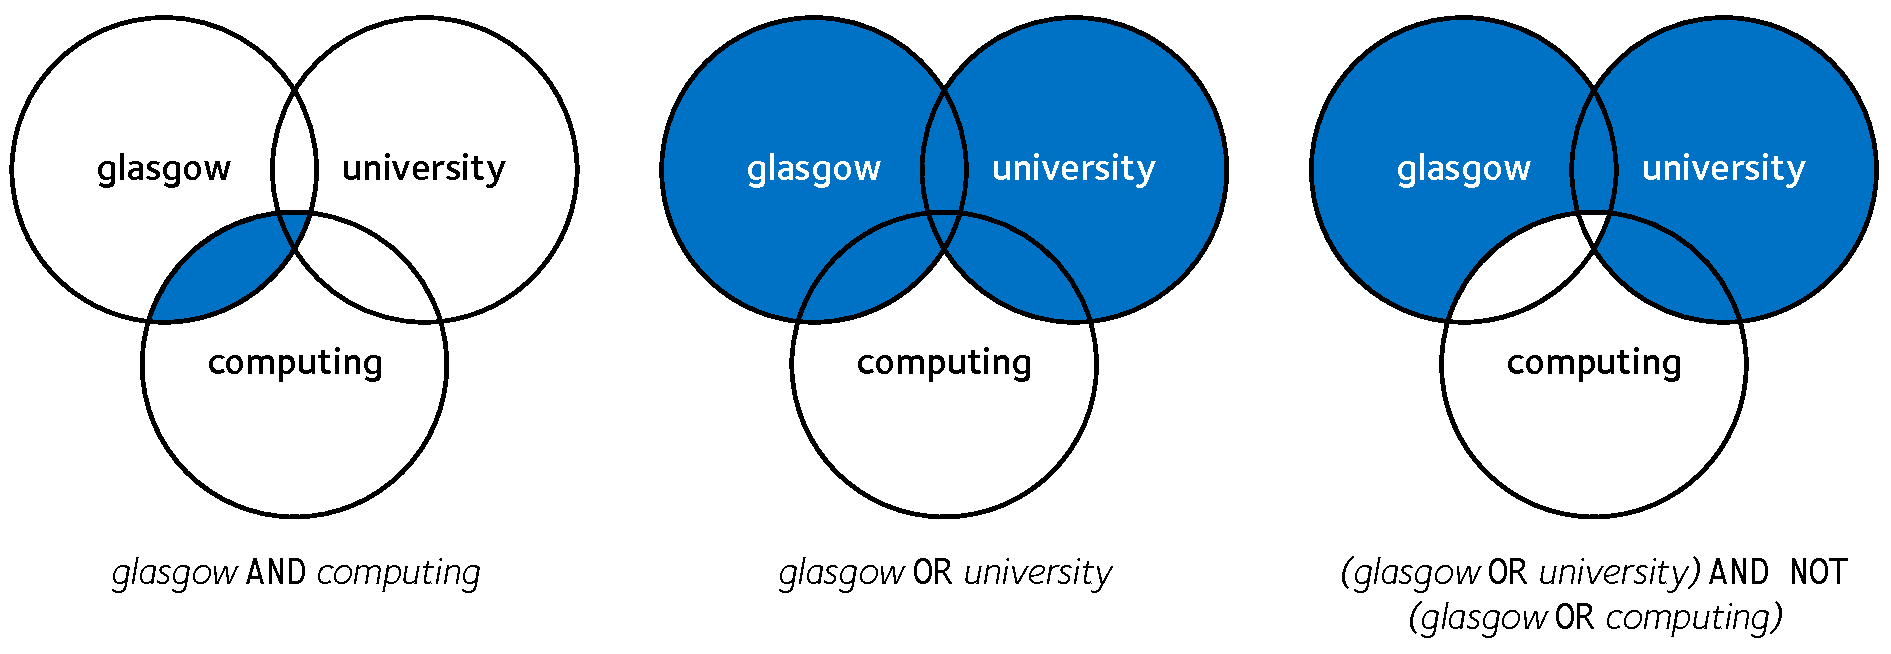
\includegraphics{figures/ch2-boolean.pdf}}
    \caption[Venn diagrams illustrating boolean retrieval]{An example illustration of the boolean retrieval model, using the query terms \texttt{glasgow}, \texttt{university} and \texttt{computing}. Each disc represents the set of documents containing that particular term. In the figure, three Venn diagram examples are provided, demonstrating the key logical operators used (\texttt{AND}, \texttt{OR} and \texttt{NOT}). Areas in blue are returned in the example boolean query provided underneath each Venn diagram.}
    \label{fig:boolean}
\end{figure}

By considering an individual query term as an unambiguous set of documents, logical operations can be applied to retrieve a set of documents. For example, the query term \texttt{glasgow} will yield a set of all documents containing the term \texttt{glasgow}, yet the query \texttt{NOT glasgow} will retrieve the set of documents that \emph{does not} contain any mention of the term \texttt{glasgow}. The results of applying logical operators between different sets can be illustrated through a Venn diagram, where each set of documents is represented as a disc. Figure~\ref{fig:boolean} provides an example of such diagrams.

Despite the relative simplicity of this approach, there are major limitations. First, when considering the query, there is no notion of term importance -- every term has equal weighting. Queries utilising logic rules also appear to be relatively unnatural representations of an information need. Indeed, as the information need become more complex, the boolean query can grow to be disproportionally large and cumbersome to interpret (refer to the right Venn diagram of Figure~\ref{fig:boolean}). This would be especially true when a complex information need is represented as a boolean query. As documents either belong to a set or they don't, a document is either useful (\texttt{TRUE}) or not (\texttt{FALSE}). As such, one cannot estimate a degree to how relevant a document would be to the searcher's query, and thus results are provided to the searcher unranked.

Returning an unranked set of documents would appear as an alien concept to users of~\gls{acr:ir} systems today -- one would assume that the document presented first would be the document considered most likely to be useful as per the underlying retrieval model. This would make it difficult for a searcher to obtain some notion of how many results he or she should examine before stopping, as all terms and documents are considered equal. Despite not being required in contemporary~\gls{acr:ir} systems, many do still provide support for crafting a boolean query for when returning a good set of results is difficult. This may for example be useful when there is ambiguity in the searcher's information need, and clarification is required to eliminate a set of unhelpful documents. Boolean queries also find traction in patent searching, where \emph{recall} rather than \emph{precision} is preferred (refer to Section~\ref{sec:ir_background:evaluation}).

\subsubsection{Vector Space Model}
With major weaknesses present in the boolean retrieval model, work then progressed to develop more advanced approaches that mitigated the issues raised above.~\cite{luhn1957ranking_query} hypothesised that a searcher, when wishing to search for documents addressing their information need, should prepare a document that is similar to the documents that were sought after. By comparing documents against this \emph{representative} document, a system could begin to deduce what other documents would be useful, and by what margin.

The vector space model proposed by~\cite{salton1975vsm} incorporates the principles as outlined by~\cite{luhn1957ranking_query}. These basic principles are operationalised by representing queries and documents within Euclidean geometry, where both are represented as vectors in multi-dimensional space. The notion of how close documents appear to each other denotes the usefulness of a document.

The vector space model is popular, as it provides an intuitive means for addressing the overarching problem of an~\gls{acr:ir} system, and can incorporate methods such as term weighting which have been shown to improve retrieval effectiveness~\citep{croft2010search}. Furthermore, as queries and terms are represented in Euclidean space, vector similarity methods can be employed to determine relevance/usefulness. While many approaches have been trialled, empirical evidence has favoured \emph{cosine similarity}~\citep{croft2010search}. This is aptly illustrated in Figure~\ref{fig:vector_space}. Using such an approach allows one to then compute the degrees of relevance/usefulness, meaning that matched documents can be returned in a ranked order. This ranking than then be potentially utilised by a searcher to determine a cutoff point at which he or she should stop examining results.

\begin{wrapfigure}[13]{r}{0.45\textwidth}
    \begin{center}
    \vspace*{-10mm}
    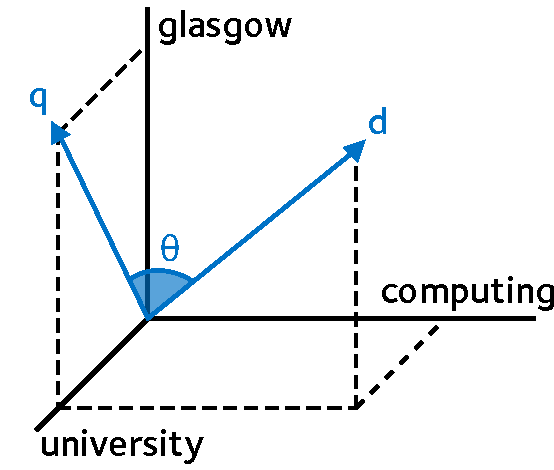
\includegraphics[width=1\textwidth]{figures/ch2-vector.pdf}
    \end{center}
    \vspace*{-4mm}
    \caption[Vector Space Model (Cosine similarity)]{An illustration of the Vector Space Model in Euclidean space, with each term representing a dimension. Here, the cosine similarity between query \emph{q} and document \emph{d} is shown.}
    \label{fig:vector_space}
\end{wrapfigure}

In order to understand the basic workings of the vector space approach, let us consider a query, $Q$, with each of its constituent terms placed within a term vector in $t$-dimensional space, leading to $Q = (q_1, q_2, q_3,\dotsc, q_{it})$. Consider also a document, $D_i$, with terms from the document again represented in $t$-dimensional space, yielding $D_i = (d_{i1}, d_{i2}, d_{i3},\dotsc, d_{it})$. From this notation, $d_{ij}$ represents the \emph{term frequency (TF)} of term $j$ appearing in document $i$. With each term represented as a separate dimension within Euclidean space, a weighting scheme can be subsequently applied to emphasise or understate more discriminative or less discriminative terms, respectively. An example of less discriminative terms would for example be stopwords, as described in Section~\ref{sec:ir_background:basics:indexing:stopwords}. By applying weighting schemes, the vector space model at a stroke overcomes a previously discussed limitation of the boolean model in that all terms are weighted equally.

Term frequency is one of many different term weighting schemes that have been trialled over the years in~\gls{acr:ir} research. Perhaps one of the best and widely used schemes is \emph{inverse document frequency (IDF)}, proposed by~\cite{sparck1972statistical}. Here, the frequency of a term is normalised against the length of a given document. In the words of its creator, IDF allows for one to define the specificity of a term as \emph{``an inverse function of the number of documents in which it occurs.''}~\citep{sparck1972statistical}. This is useful as non-discriminative terms that occur frequently within an index (e.g. \texttt{the}) would have its weight diminished, with the inverse happening for more discriminative terms, better able to describe a given document.

TF and IDF are typically combined together as a measure of both term appearance and importance, under an approach called \emph{TF-IDF}. For a given term $k$, one can calculate a TF-IDF score with the following equation:

\begin{equation*}
tf_{i,k} \cdot idf_{k} = \frac{f_{i,k}}{\sum_{j=1}^{t} f_{i,j}} \cdot log \frac{N}{n_k}.
\end{equation*}

Above, $f_{i,k}$ is the frequency of term $k$, $N$ is the number of documents in the collection used, and $n_k$ is the number of documents in which term $k$ appears at least once.

\subsubsection{Probabilistic Models}
From boolean to vector space retrieval models, a further model emerged based upon \emph{probability theory}. Probability theory allows one to define a means to formally model the relevance and/or usefulness of a document to a searcher's query, given \emph{uncertainty} about their precise information need. One of the most widely referred to ranking principles, known as the \emph{Probability Ranking Principle (PRP)} (defined by~\cite{robertson1977prp} -- who in turn attributed the development to~\cite{cooper1971relevance}), states the following.

\begin{quote}
\emph{``If a reference retrieval system's response to each request is ranking of the documents in the collections in order of decreasing probability of usefulness to the user who submitted the request, where the probabilities are estimated as accurately as possible on the basis of whatever data has been made available to the system for this purpose, then the overall effectiveness of the system to its users will be the best that is obtainable on the basis of that data.''}
\attrib{\cite{robertson1977prp}}
\end{quote}

Essentially, this states that documents that are considered more likely to be relevant than non-relevant should be retrieved -- or where $P(R|D) < P(\overline{R}|D)$. However, while the PRP lays much of the foundation from which probabilistic retrieval models have been derived, it does not itself provide a concrete implementation of such a model. The framework provided by the PRP in order to score a document to a searcher's query is:

\begin{equation*}
score(d,q) = P(rel|q,d) \approx \sum_{t \in q}wt_{t,d}.
\end{equation*}

Above, $rel$ is defined as the relevance probability of document $d$, given query $q$. Early approaches following this framework utilised Bayes' theorem to define the probability of a document being relevant to the associated query, based upon the likelihood of drawing query terms from relevant and non-relevant documents. This was considered as a classification problem, where documents were considered as either relevant or non-relevant to said query. The aforementioned likelihood has been computed by many models -- perhaps the most important being \emph{Okapi BM25}~\citep{robertson1995trec3}. Indeed, this retrieval model has had considerable impact upon the~\gls{acr:ir} community and is still used extensively today, providing a solid baseline for contemporary research. This model is employed as the basic retrieval model for experimentation in this thesis due to its effectiveness and popularity.

\subsubsection{Language Models}
The final retrieval model family that we discuss are language models, closely related to the probabilistic model we define above. Indeed, while such probabilistic models have been demonstrated to perform well empirically, adapting the PRP and subsequent developments to more advanced approaches has been difficult and is generally not intuitive~\citep{hiemstra2000language_modelling} -- the interpretation offered by probabilistic models may be considered loose, and is not always theoretically principled~\citep{whiting2015phd}. This has led to the development of more formalised statistical language modelling approaches, as defined in the fields of \emph{Natural Language Processing (NLP)}, for example~\citep{lavrenko2001language_models}.

Given the strong rooting in the principles of language and associated fields, language models provide a solution to the so-called \emph{bag of words}~\citep{harris1954distributional} concept that a majority of preceding retrieval models subscribe to. Put simply, this concept considers each document and query as a bag of words, meaning that the ordering of terms loses any significance. While a simplifying assumption, losing the ordering of terms means that semantic meaning and grammar rules are lost -- and thus a retrieval engine employing a model using this simplifying assumption may lose key meanings, and subsequently retrieval effectiveness will suffer.

Essentially, a language model is a probability distribution over strings of text. Given a string of text (i.e. a searcher's query), how likely is it that the given query appears in a given \emph{language}? Each document provides its own language, where we consider all possible phrases that the author of a document could have written when creating said document. Of course, some phrases are more likely than others. For example, the phrase \texttt{rain in glasgow} is more likely to appear in a document (in that order) than the seemingly random assortment of terms \texttt{purple monkey dishwasher}\footnote{If you ever watched \emph{The Simpsons}, you might disagree with this statement.}. Given this, and conceptualising a searcher's query in much the same fashion, we can produce a probability distribution $P(Q|D)$, concerning the probability of observing query $Q$ during some form of sampling within the language model of document $D$.

The most simplistic approach to language modelling is undoubtedly the \emph{unigram} approach, where each term within a document and/or query are considered in isolation, which subscribes to the aforementioned simplifying bag of words concept. Essentially, such an approach provides a probability distribution over the words appearing in the language. Higher order \emph{grams} such as \emph{bi-grams} and \emph{tri-grams} begin to consider more the place in which terms appear with respect to others, and thus the semantic meaning defined by this positioning begins to be taken into account within the probability distribution. When considering a document, the more a document discusses a particular topic, the more likely one would begin to observe terms about that topic in said document. When a term is not mentioned in a document, smoothing can be applied (given the wider collection the document is part of) to avoid a zero probability when calculating the probability of terms permitting the partial matching of queries where not all terms appear within a target document.

\subsection{Evaluating Systems}\label{sec:ir_background:evaluation}
Given the \emph{de facto} architecture of an experimental~\gls{acr:ir} system (Section~\ref{sec:ir_background:basics:cranfield}) and the numerous retrieval models that one can employ (Section~\ref{sec:ir_background:basics:models}), how can we then begin to evaluate a given retrieval system? Recalling that the \emph{modus operandi} of such a system is to satisfy the needs of the searchers who utilise it,~\cite{lancaster1968information} provides three criteria by which an~\gls{acr:ir} system can be evaluated:

\begin{itemize}
    \item[\emph{(i)}]{the suitability of an~\gls{acr:ir} system in terms of the specific tasks for which it will be used;}
    \item[\emph{(ii)}]{the~\gls{acr:ir} system's task performance \emph{efficiency}; and}
    \item[\emph{(iii)}]{the extent to which the system satisfies the information needs of its \emph{users.}}
\end{itemize}

These three criteria can themselves be subsequently split into two separate categories: approaches that consider how well the \emph{system} performs (i.e. criterion \emph{(i)} and \emph{(ii)}); and with regards to the individual who is using the~\gls{acr:ir} system at the time (\emph{user-orientated}, criterion \emph{(iii)})~\citep{voorhees2005trec_book}. Given the title of this section, we subsequently only consider system-orientated evaluation approaches here; a more detailed explanation of a user's role and how we can evaluate their performance is provided in Section~\ref{sec:ir_background:user:evaluation}.

Considering system-orientated measures of evaluation, one can consider a system's \emph{efficiency} or \emph{effectiveness}. Efficiency concerns some form of operational metric, such as the speed of the~\gls{acr:ir} system. This example is important (especially in commercial web search engines) as even a fractional increase of the time taken to return results to a searcher can reduce the number of returning searchers, and impacts search engine revenue~\citep{brutlag2009speed}. Indeed, this is examined in more detail in Chapter~\ref{chap:temporal}.

However, when one thinks of~\gls{acr:ir} evaluation, they usually think about how \emph{effective} the system is. Of course, the definition of what defines an~\gls{acr:ir} system to be effective hugely depends upon the type of search task being undertaken. A patent searcher would for example expect an~\gls{acr:ir} system to return \emph{all} relevant patents to avoid missing a related patent (and thus incurring penalties) -- whereas a casual web searcher curious about a topic they know little about (i.e. ad-hoc) would be satisfied with a single, relevant result.

As such, this section provides a brief overview of the basic effectiveness measures widely used within~\gls{acr:ir} today. We consider four different measures. It should be noted that such measures are usually computed from \emph{batch-style} experimentation with up to $1,000$ results available to obtain the best approximation possible.

\begin{figure}[t!]
    \centering
    \resizebox{1\hsize}{!}{
    
\includegraphics{figures/ch2-pr.pdf}}
    \caption[Precision and recall]{An illustration of precision and recall. On the left is an illustrated example of an index, containing many documents. The large circle represents the set of documents retrieved for a query. Documents that are relevant to the query are represented as~
\includegraphics[height=\fontcharht\font`\d]{figures/ch2-pr-r.pdf}, with non-relevant documents represented as~
\includegraphics[height=\fontcharht\font`\d]{figures/ch2-pr-nr.pdf}. Note that not all relevant documents are retrieved; doing so would mean that the retrieval engine used would have produced perfect results. From the illustration on the left, definitions of \emph{precision} and \emph{recall} are also provided.}
    \label{fig:pr}
\end{figure}

\subsubsection{Precision}\label{sec:ir_background:evaluation:precision}
The \emph{precision} ($P$) of an~\gls{acr:ir} system considers the fraction of documents that have been retrieved that are considered to be relevant or useful to the searcher's given query, information need. An~\gls{acr:ir} system that yields high precision is regarded as one that performs well.

Figure~\ref{fig:pr} provides a visual illustration of what precision entails (as well as its counterpart, \emph{recall}, which is discussed below). Given the set of all documents within an index, an~\gls{acr:ir} system will retrieve a number of these documents that satisfy the criteria set out in the retrieval model employed. Of the documents retrieved, some will be considered relevant to the searcher's information need; others will be considered non-relevant. As such, prior knowledge of the relevance of particular documents to given topics is therefore required (e.g. TREC QRELs, as defined in Section~\ref{sec:ir_background:basics:cranfield:trec}).

Precision can therefore be defined as:

\begin{equation*}
precision = \frac{|~\text{\emph{relevant documents}}~\cap~\text{\emph{retrieved documents}}~|}{|~\text{\emph{retrieved documents}}~|}.
\end{equation*}

Research in~\gls{acr:ir} typically reports precision up to a particular rank, i.e. $P@k$. For example, $P@10$ will provide a fractional value for the number of relevant documents that appeared within the top $10$ results of a query. Herein lies one of the most elementary and basic \emph{stopping models} that we find encoded within various measures and models defined by~\gls{acr:ir} researchers over the years -- stopping at $10$\footnote{The value of $k=10$ is often chosen in~\gls{acr:ir} research as it has been shown that this is typically the depth to which searchers would look through web search results~\citep{jansen2006www}.}, or $k$, denotes that a system or searcher need not bother examining any further documents.

\subsubsection{Recall}
While precision considers the fraction of documents retrieved that are relevant, \emph{recall} ($R$) considers the fraction of documents that were retrieved and relevant to a query against \emph{all known relevant documents for a query}. Recall can formally be defined as:

\begin{equation*}
recall = \frac{|~\text{\emph{relevant documents retrieved}}~|}{|~\text{\emph{relevant documents}}~|}
\end{equation*}

Considering the patent searching example defined above, high recall would be desirable in this type of task -- high recall means more patents matching the searcher's query will be returned, thus reducing the possibility of missing important prior filings.

Given more modern retrieval models, the notion of ranking would lead a searcher to assume (as per the PRP~\citep{robertson1977prp}) that relevant documents pertaining to their query will be the first results presented. Non-relevant documents will also of course appear, typically leading to some form of tradeoff between precision and recall, as discussed below. The tradeoff considers the notion that as you increase recall, the number of non-relevant items will undoubtedly also increase, thus reducing the~\gls{acr:ir} system's overall precision.

\subsubsection{F-Measure}
Considering the aforementioned tradeoff between precision and recall, the \emph{F-measure}, which represents a \emph{weighted, harmonic mean} between the two. Originally proposed by~\cite{rijsbergen1979ir}, the measure was provided to \emph{``measure the effectiveness of retrieval with respect to a user who attaches $\beta$ times as much importance to recall as precision.''} The F-measure, along with its $\beta$ parameter, is defined by~\cite{chinchor1992f_measure} as:

\begin{equation*}
F_\beta = \frac{(\beta^2 + 1)\cdot PR}{\beta^2 \cdot P + R}\hspace{10mm}(0\leqslant\beta\leqslant+\infty).
\end{equation*}

Above, $P$ and $R$ denote precision and recall respectively. $\beta$ is simply used as a parameter for controlling the balance between the two. When $\beta = 1$, $F_1$ is equivalent to the harmonic mean of precision and recall. Since the terms F-Measure and harmonic mean are ubiquitously linked (somewhat \emph{harmoniously}\dots), the two terms are used interchangeably within the literature. As $\beta$ tends towards $0$, the score becomes more precision orientated.

\begin{figure}[t!]
    \centering
    \resizebox{1\hsize}{!}{
    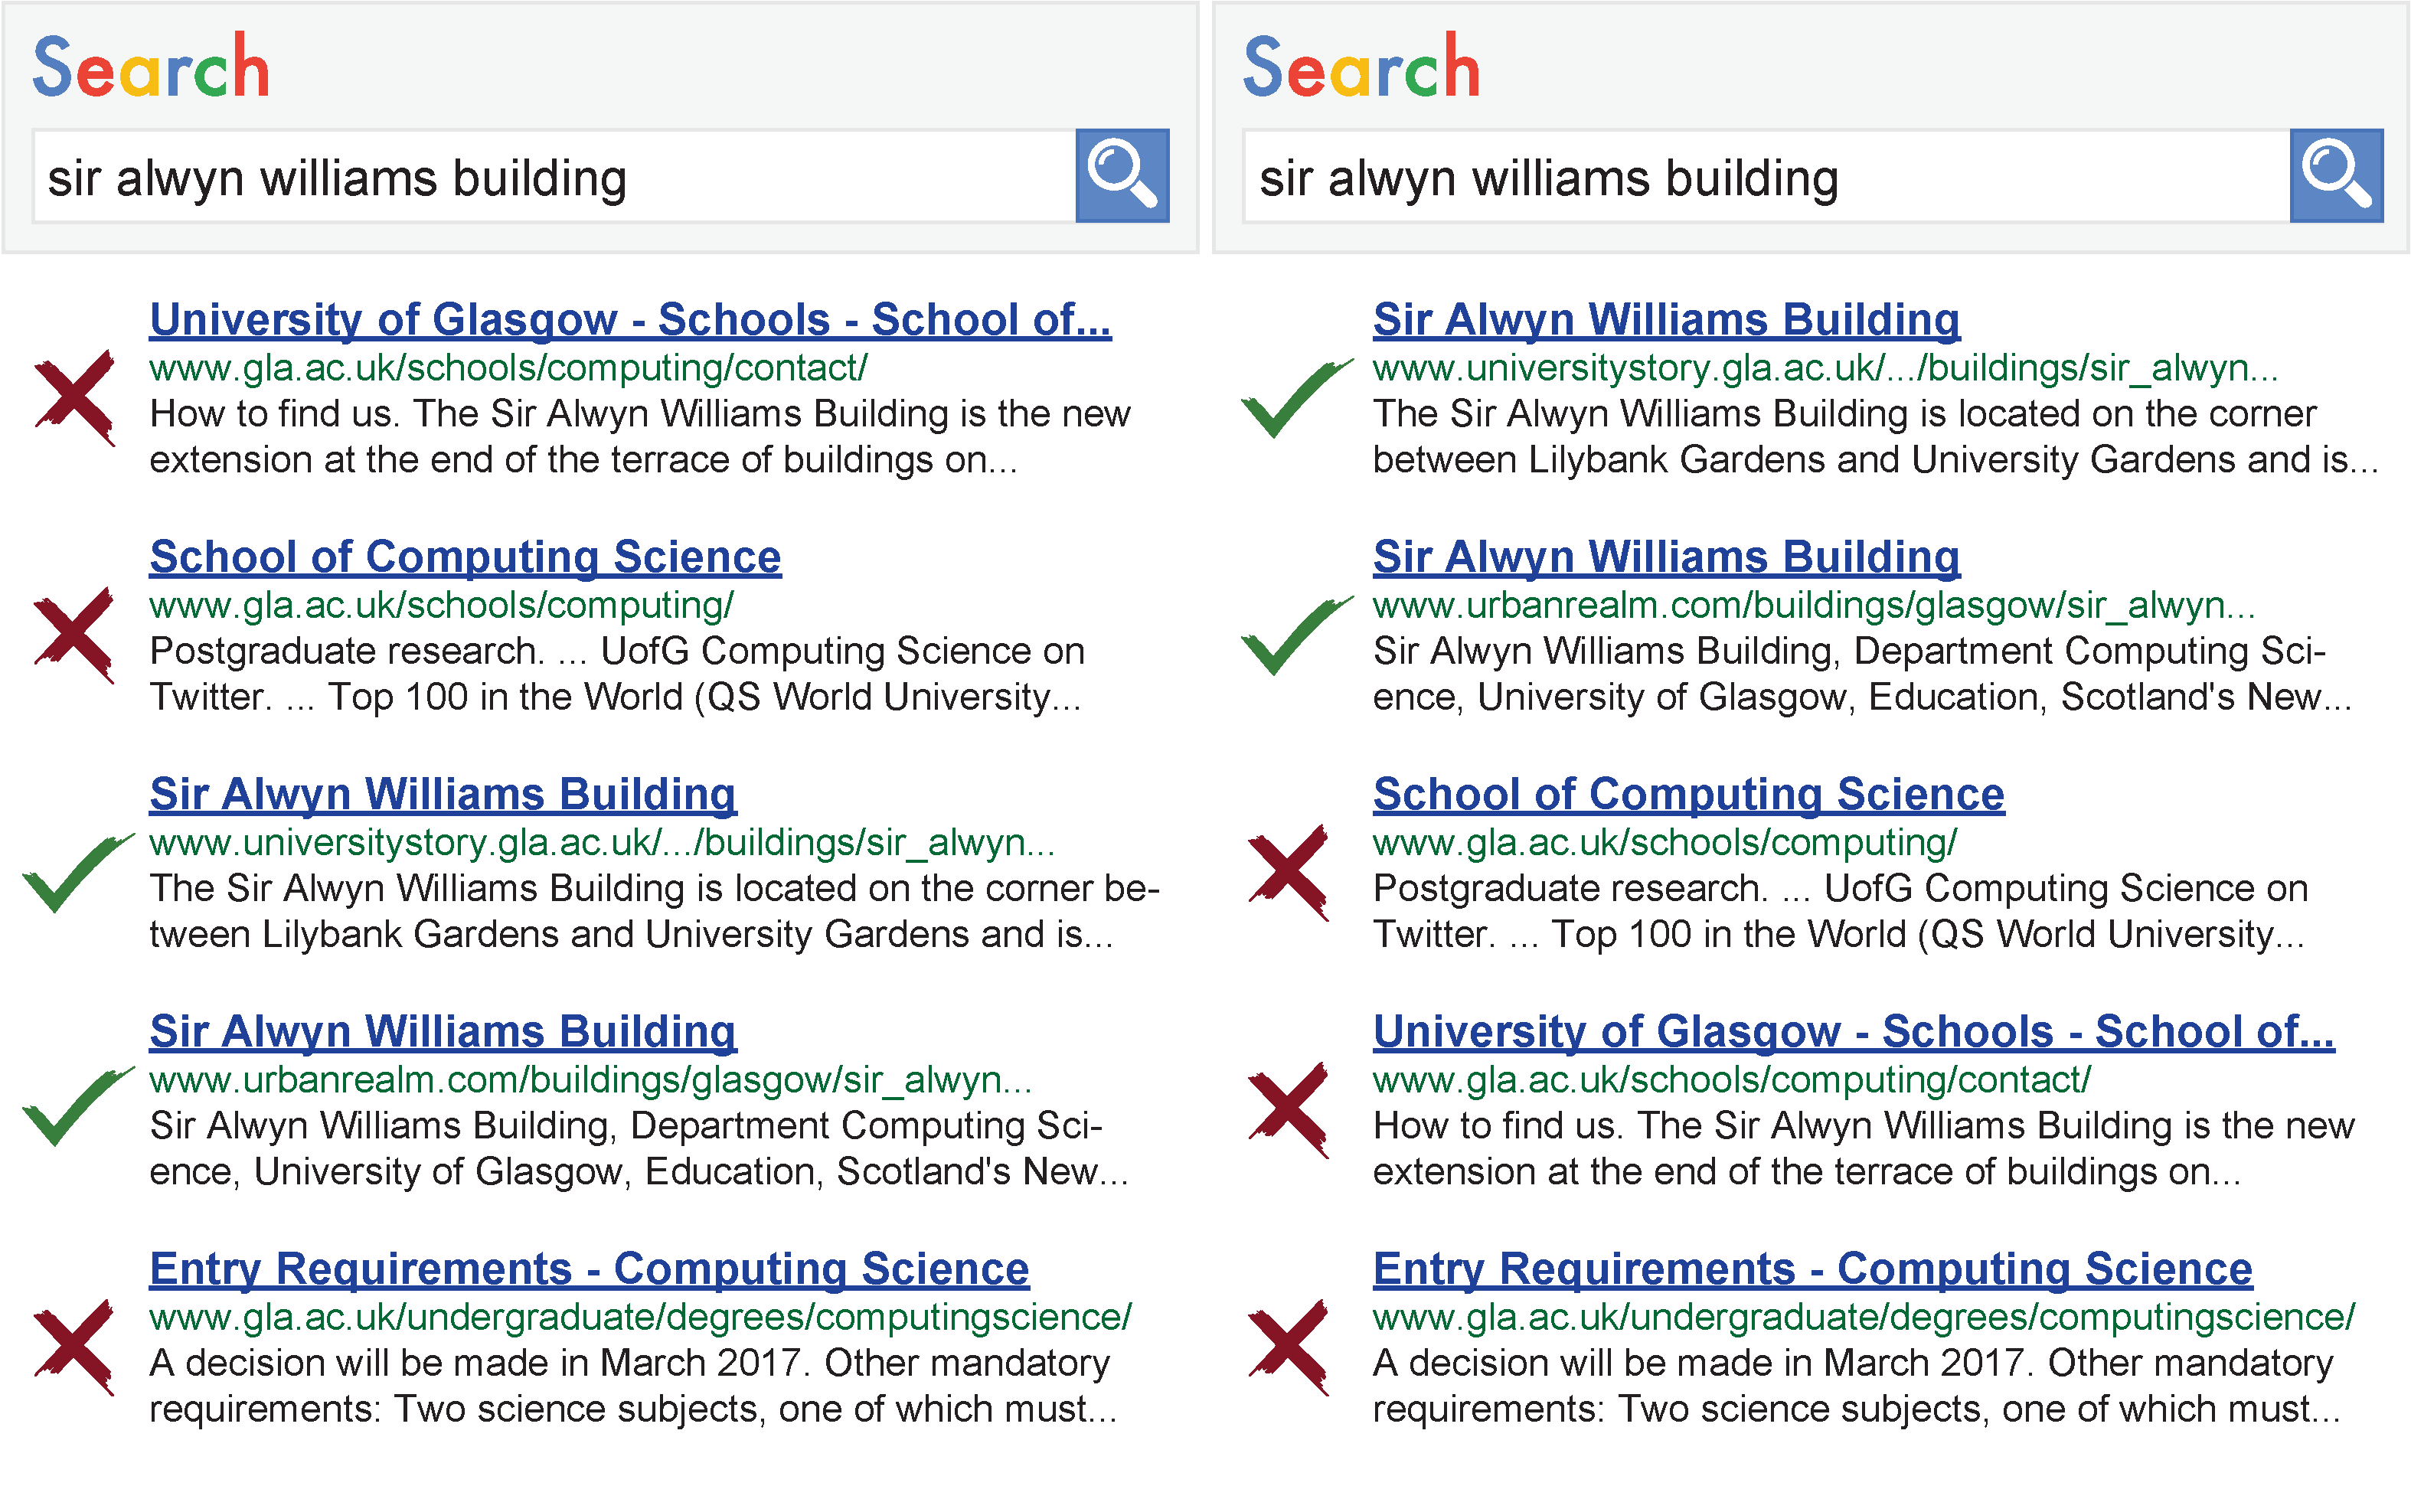
\includegraphics{figures/ch2-ranking.pdf}}
    \caption[The importance of ranking]{Given an information need to find out information about the \emph{Sir Alwyn Williams Building} (part of the University of Glasgow's estate portfolio), which ranked list of results would you prefer to make use of?}
    \label{fig:ranking}
\end{figure}

\subsubsection{Mean Average Precision}
One of the major limitations of the previously examined measures is that the \emph{ranking} of results is not specifically taken into consideration. For example, consider Figure~\ref{fig:ranking}. Looking at the {\color{dmax_green}ticks} and {\color{dmax_red}crosses} (denoting relevant and non-relevant content, respectively) within the figure, would it be desirable to be presented with the list of results ranked in order shown on the left, or on the right? Despite apparent differences in the ranking of results, precision for example would show no difference -- both ranked lists contain two relevant documents, and three non-relevant. A simple calculation would show that the $P@5$ score for both lists would therefore be $2 / 5 = 0.4$ -- there is no discernible difference between them.

One of the most widely used measures that addresses this issue -- and provides a means of quantifying the all-round effectiveness of a retrieval system for a representative set of test topics -- is \emph{Mean Average Precision (MAP)}~\cite{voorhees2005trec_book}. Rather than considering a single set of results, MAP can consider multiple queries -- and, as alluded to above, considers the ranking in which results for each query are provided.

As the name might imply, MAP provides a mean over the \emph{Average Precision (AP)} for each topic that is examined. AP provides the rank sensitive component of MAP up to some cuttoff $k$, as defined below:

\begin{equation*}
AP = \frac{\sum^{n}_{k=1}(P(k) \cdot rel(k))}{|~\text{\emph{relevant documents}}~|}.
\end{equation*}

Above, $P(K)$ is the precision cutoff at rank $k$ (i.e. $P@k$), and $rel(k)$ is a function to denote the relevance of a particular document at rank $k$. This is assumed to be binary, with $1$ denoting a relevant document, and $0$ denoting a non-relevant document. AP is then computed for each sample query, $q$, over the set of topics $T$ to produce a final MAP score for the~\gls{acr:ir} system:

\begin{equation*}
MAP = \frac{\sum^{T}_{q=1} AP(q)}{|~Q~|}.
\end{equation*}


\section{Considering the User}\label{sec:ir_background:user}
So far in this chapter, we have provided a background on several key developments in the area of~\gls{acr:ir} research. However, these aforementioned developments all purely consider the \emph{system} that is being evaluated (i.e \emph{system-sided} research). To reiterate once more, the overall goal of an~\gls{acr:ir} system is to satisfy some information need that a searcher, or \emph{user}, acquires. In short, satisfying the user is key to~\gls{acr:ir}. Central to this is our understanding and incorporation of a user's search behaviours and interactions into the evaluation of~\gls{acr:ir} systems~\citep{callan2007minds}.

The study of~\glsfirst{acr:iir} attempts to address this gap in our collective knowledge.~\gls{acr:iir} studies can include aspects from user-sided and system-sided research. For example, one might present results of a user study examining a particular phenomenon of a user's behaviour, and also provided details of a system-sided evaluation. As discussed by~\cite{kelly2009iir},~\gls{acr:iir} can trace its roots back to a variety of different disciplines, including: traditional~\gls{acr:ir}; library and information science; psychology; and~\gls{acr:hci}. Typically presented as branch of~\gls{acr:ir} and/or~\gls{acr:hci}, arguments also exist to consider~\gls{acr:iir} as a distinct area of research~\citep{ruthven2008iir}.

\begin{quote}
\emph{``In~\gls{acr:iir}, users are typically studied along with their interactions with systems and information. While classic~\gls{acr:ir} studies abstract humans out of the evaluation model,~\gls{acr:iir} focuses on users' behaviors [sic] and experiences -- including physical, cognitive and affective -- and the interactions that occur between users and systems, and users and information. In simple terms, classic~\gls{acr:ir} evaluation asks the question, does this system retrieve relevant documents?~\gls{acr:iir} evaluation asks the question, can people use this system to retrieve relevant documents?''}
\attrib{\cite{kelly2009iir}}
\end{quote}

In order to aptly describe where~\gls{acr:iir} fits into the system-sided vs. user-sided space,~\cite{kelly2009iir} also provided an intuitive spectrum of work in this area, comprised of eight types of study -- as shown in Figure~\ref{fig:spectrum}. Below, we provide a brief explanation of the key types of study as shown in the spectrum.

\begin{figure}[t!]
    \centering
    \resizebox{1\hsize}{!}{
    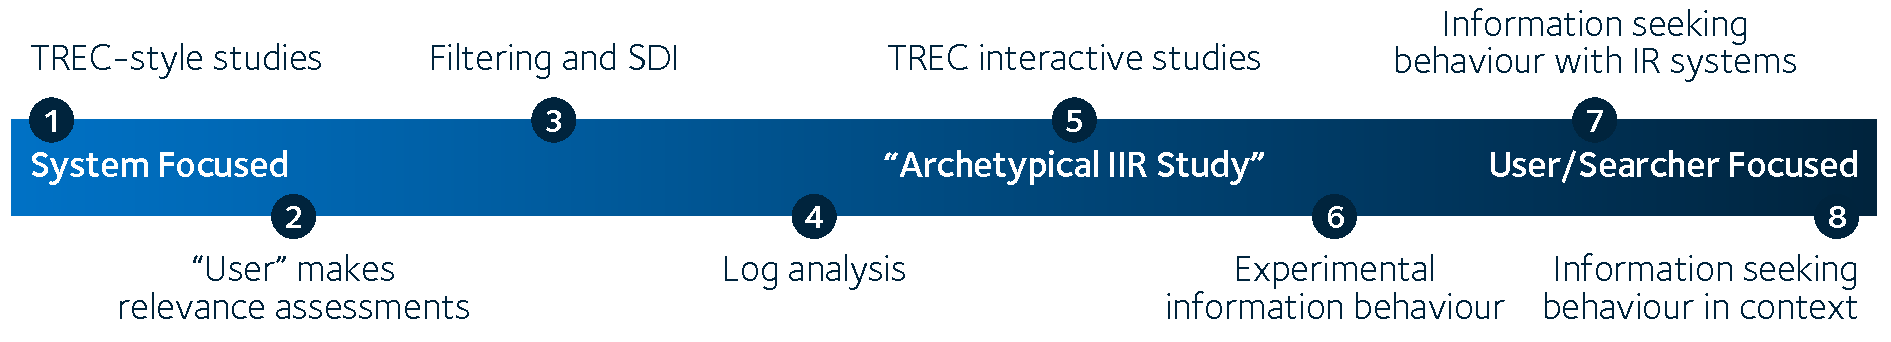
\includegraphics{figures/ch2-spectrum.pdf}}
    \caption[Spectrum IIR research~\citep{kelly2009iir}]{The spectrum of conceptualising IIR research. Methods on the left consider a more system-focused approach, with those on the right considering a more user-focused approach. The fifth step within the spectrum considering TREC interactive studies is considered to be an \emph{"archetypical~\gls{acr:iir} study"}. Figure adapted, with permission, from~\cite{kelly2009iir}.}
    \label{fig:spectrum}
\end{figure}

\begin{itemize}
    
    \item[\emph{(1)}]{\blueboxbold{TREC-style studies} focus on the development and evaluation of system-sided research, such as retrieval models and indexing methods. These would be considered akin to most of the studies undertaken in TREC tracks over the years (excluding tracks such as the Interactive Track, for example). No real users are utilised using this approach, although we do argue that there is a simplistic \todo{\emph{user model}} encoded within this approach. Human assessors however create judgements used for evaluation, but they do not function as searchers as such. Assessors are the only humans \emph{in the loop} for this type of study -- the rest is fully automated on computers.}
    
    \item[\emph{(2)}]{\blueboxbold{'User' relevance assessment studies} do consider humans \emph{in the loop}, but this time for exceptionally limited purposes. As the name for these studies may suggest, humans are employed for generating relevance assessments as part of the study, and as such, no searching takes place.~\cite{bota2016cards} undertook a study of this nature, where they examined search behaviour for predefined queries when presented with a series of \emph{information cards}\footnote{An \emph{information card} is a contemporary feature of a~\gls{acr:serp}, typically presented on the right rail of the page. They provide additional information to the topic in question, such as images and basic statistics of the entity.}}.
    
    \item[\emph{(5)}]{Moving along the spectrum,~\cite{kelly2009iir} cites~\blueboxbold{TREC interactive studies} in which typically a system and/or interface feature is evaluated. Typically, the feature is related to the human, such as examining their behaviour, cognition or information seeking context. These studies usually aim to assist in aiding our understanding of the search process, and to aid in the development of more intuitive and user-friendly search interfaces.}
    
\end{itemize}

The studies complying with point \emph{(5)}, called \emph{archetypical~\gls{acr:iir} studies}~\citep{kelly2009iir}, are the studies which we largely consider in this thesis -- indeed, later on in this thesis, we consider a variety of aspects that can influence the behaviour and performance of searchers. Moving further along the spectrum, the study of users becomes ever more prominent, until we reach:

\begin{itemize}
    
    \item[\emph{(8)}]{\blueboxbold{information seeking behaviour in context studies} which considers research that (almost) exclusively focuses on users. Here, we consider the information needs of the individuals~\gls{acr:ir} systems aim to satisfy -- searchers. Researchers typically would examine a user search, while collating qualitative data about their experiences.}
    
\end{itemize}

Of course, a more detailed explanation of these different types of study can be found in the work by~\cite{kelly2009iir} that illustrate the more user-centric approaches in detail. We now however turn our attention back to the idea of employing simulation and a form of \emph{user model} in order to better understand a searcher's complex interactions during the search process.

\subsection{Considering User Models}
Models of the search process attempt to capture the high level, cognitive processes that a searcher undertakes during a search session -- such as issuing a query, or examining a document for relevance. User models of the search process have been present in more system sided~\gls{acr:ir} research for a number of decades (as discussed in Section~\ref{sec:ir_background:user}), as well as implicitly encoded within the variety of measures that have been used.

\cite{carterette2011models} argues that the measures widely used within the~\gls{acr:ir} community are themselves typically comprised of three, distinct underlying models:

\begin{enumerate}
    \item{a \emph{browsing model}, describing how a searcher interacts with a search engine and the subsequent~\glsplural{acr:serp} that are presented to them;}
    \item{a model encoding some form of \emph{document utility} that provides a description for how utility can be derived from relevant documents; and}
    \item{a \emph{utility accumulation model} that describes how a searcher accumulates utility over the course of a search session.}
\end{enumerate}

Of particular interest to the work in this thesis are the \emph{browsing models} that attempt to capture the broad interactions that take place between the searcher and the search engine. One of the most well developed browsing models highlighted by~\cite{carterette2011models} is that of a searcher, after issuing a query, examines a series of documents presented to him or her on the resultant~\gls{acr:serp} one by one (in a linear fashion), and at some depth, $k$, stops. This is the basic model followed by measures such as $P@k$, for example. (refer to Section~\ref{sec:ir_background:evaluation:precision}). This process is illustrated with a flowchart in Figure~\ref{fig:basic_model}.

\begin{figure}[t!]
    \centering
    \resizebox{1\hsize}{!}{
    \includegraphics{figures/ch2-basic_model.pdf}}
    \caption[A basic user model of search]{A basic model of the search process. Here, a searcher, after issuing a query to the underlying search engine, examines a number of different items presented to him or her before deciding to stop at some rank \emph{k}. This basic approach is widely used in many measures of~\gls{acr:ir} effectiveness, and is considered by~\cite{carterette2011models} as a form of \emph{browsing model}, capturing the interactions that take place between the searcher and search engine.}
    \label{fig:basic_model}
\end{figure}

While perhaps deficient in terms of representing a real-world searcher's behaviours, this basic model has served the~\gls{acr:ir} community well for a number of decades, and works well in batch-style experimentation that is common in the community. While more advanced models of the search process have been developed, we leave these to Section~\ref{sec:stopping_background:models:conceptual}. Instead, we now consider the notion that with a user model of the search process, we can then take this model to provide a \emph{simulation} of the interactions that take place.

\subsection{Simulation in~\gls{acr:ir} and~\gls{acr:iir}}\label{sec:ir_background:user:simulation}
As outlined in Section~\ref{sec:intro:motivation}, employing simulation for~\gls{acr:iir} studies in conjunction with a model of the search process allows for consistent and reproducible results. Several user models exist; one of the most widely used and simplistic approaches considered is the TREC-style user model, as detailed in Section~\ref{sec:stopping_background:models:conceptual:trec}. Simulation however is not exclusively used for modelling searcher behaviours -- in traditional~\gls{acr:ir}, simulation has been used for example in simulated work tasks~\citep{borlund2003iir_model, voorhees2005trec_book}, simulated and synthetic data collection~\citep{azzopardi2009query_side, azzopardi2007languages, jordan2006cqg, tague1980simulation_bibliographic}, and the simulation of interaction~\citep{azzopardi2010workshop, carterette2011effectiveness_evaluation, clarke2013mube,  leuski2000relevance_reinforcement, white2004simulated_feedback_models}.

There has also been a growing interest with the simulation of interaction, and in particular how to model searcher behaviour~\citep{azzopardi2010workshop, clarke2013mube}. This is for a variety of reasons. Firstly, simulation provides a cost effective means of evaluation which is reliable, repeatable and therefore reproducible. Secondly, most, if not all evaluation measures either implicitly or explicitly encode some form of user model (typically a stopping model) in order to make measurements. Simulation also provides a means in which to explore different searcher behaviours, methods and techniques to better understand how searchers do, could, or are likely to behave. However, if simulations are not properly grounded, motivated and validated, the findings from such simulations can be considered questionable. Thus, there is a pertinent need to ensure that the models developed are credible abstractions of the search process, and that they are seeded with data based on actual human interaction data~\citep{azzopardi2010workshop}\footnote{\scriptsize{The exception being when exploratory simulations are conducted to examine \emph{`what-if'} scenarios.}}. 

Simulation has been used to examine a range of factors within the~\gls{acr:iir} process, usually independently, such as: query formulation and suggestions~\citep{azzopardi2009query_side, azzopardi2007languages, baskaya2013behavioural_factors, carterette2015test_collections, jordan2006cqg, keskustalo2008user_simulation, verberne2015personalised_queries}; browsing behaviours~\citep{carterette2015test_collections, chuklin2015click_models, guo2009click_chain, pakkonen2015behavioural_dimensions, smucker2011user_strategies}; relevance feedback~\citep{harman1992rf, jarvelin2009graded_relevance, keskustalo2006rf, keskustalo2008user_simulation, ruthven2003interactive_query_expansion}; the influence of costs and time~\cite{azzopardi2011economics, baskaya2012simulating_sessions}; stopping strategies and stopping models~\cite{carterette2011effectiveness_evaluation, carterette2015test_collections, maxwell2015initial_stopping, maxwell2015stopping_strategies, thomas2014modelling_behaviour}; and performance over sessions~\citep{luo2014winwin,luo2015pomdp}.

To undertake the aforementioned simulated studies, either \emph{(i)} the simulated component itself is considered in isolation (e.g. evaluating the performance of individual query generation techniques~\citep{azzopardi2007languages, jordan2006cqg}), or \emph{(ii)} a simulation of the entire search process is performed. Here, a simulated user is instantiated and undertakes a series of interactions, typically based upon a predefined search process until they reach a certain level of gain, reach a time limit, or meet some other stopping condition~\citep{baskaya2013behavioural_factors, maxwell2015initial_stopping, maxwell2015stopping_strategies, moffat2013users_versus_models, thomas2014modelling_behaviour}.

So, how do individuals actually interact with a ranked list? When, for example, do they stop examining results? In thesis, we address this question by employing a hybrid approach of conducting user studies to assist in the development of a more advanced, realistic user model that considers the search process. This model is thus guided by the findings of the user studies, as discussed in subsequent chapters~\ref{chap:temporal},~\ref{chap:snippets}, and~\ref{chap:diversity}. This model can then be tested by simulating a more complex user with weaker assumptions, thus moving the area of user modelling forward.

\subsection{Evaluating User Performance}\label{sec:ir_background:user:evaluation}
With the basic~\gls{acr:ir} measures described in Section~\ref{sec:ir_background:evaluation} consider system-sided aspects, we must also consider a number of key measures used within~\gls{acr:iir} studies. This section discusses six different measures, each with a short description of each. It may be interesting to note that a large number of measures for~\gls{acr:iir} have been proposed over the years (and indeed, over the experimental spectrum as shown in Figure~\ref{fig:spectrum}); however, only a small number of measures have been consistently used. For a more in-depth summary of measures that are available, consult~\cite{su1992iir_measures}, and more recently,~\cite{kelly2009iir}.

In addition to the spectrum of~\gls{acr:ir}/\gls{acr:iir} experimentation,~\cite{kelly2009iir} also provides a taxonomy of the different types of measures used within~\gls{acr:iir} experimentation. The taxonomy consists of four main categories that are enumerated below.

\begin{itemize}
    
    \item{The first category considers \blueboxbold{contextual} factors related to a subject of an~\gls{acr:iir} experiment. Factors include those commonly gathered from some form of demographics survey, such as the subject's age, sex, and prior search experience. In an information seeking context, one may also be able to gather information about a subject's prior knowledge, for example, on the topic they are asked to find information for.}
    
    \item{\blueboxbold{Interactions} are the second category. These measures characterise the interactions that take place between the system and the user -- including their behavioural characteristics. Examples of such interactions include: the number of queries that the user issues; the number of documents they examine; the depth to which they examine results; and the mean length (in terms) of the queries that they issue. Time-based measures are also included in this category -- both at a gross level (i.e. the total session time) and at a more specific level (i.e. the mean time spent entering queries). These measures can usually be computed by extracting and parsing interaction \emph{log data}\footnote{By \emph{log data}, we refer to the file that is created by an experimental system as a subject conducts a search task. Typically, a series of different actions (i.e. issuing a query, clicking a document link) are logged, and post-hoc log parsing can then extract this data.}.}
    
    \item{The third category considers \blueboxbold{performance} factors. As the name suggests, these measures are related to the outcome of the interactions that take place between the user and the system. These measures can be considered analogous to the system-sided measures that we examined previously in Section~\ref{sec:ir_background:evaluation}. Typically, such measures can again be extracted from interaction log data.}
    
    \item{Finally, \blueboxbold{usability} measures are typically a series of qualitative and quantitative approaches for capturing a subject's feelings and attitudes towards a search system that they have just used. Common measures in this category include the subject's view of the system's \emph{effectiveness} and their overall \emph{satisfaction} with how they performed when undertaking the search task in question~\citep{hornbaek2006usability}.}
    
\end{itemize}

When considering the work in this thesis, we employ measures from \emph{all four} of the above taxonomy's categories -- including extracting interaction data from user studies, which is subsequently employed to \emph{ground} simulations of interaction (as described in Section~\ref{sec:ir_background:user:simulation}). While contextual, interaction and usability measures are relatively straightforward to explain, we discuss in the remainder of this section a number of \emph{performance} measures that are employed in work discussed later on in this thesis.

\subsubsection{Interactive Precision and Recall}\label{sec:ir_background:user:evaluation:interactive_pr}
In Section~\ref{sec:ir_background:evaluation}, we discussed the notion that many of the system-sided evaluation measures highlighted typically are evaluated with up to $1,000$ results per query. In the real world, users of commercial web search engines have typically shown to examine to approximately only $10$ results~\citep{jansen2006www} -- perhaps due to the effects of pagination. Indeed, the notion of a subject taking part of an~\gls{acr:iir} experiment examining up to $1,000$ results for each query issued is particularly unrealistic.

Subjects of~\gls{acr:iir} experimentation also typically instructed to save documents that they consider relevant to the given information need. As such, the judgements created by subjects of~\gls{acr:iir} studies may not match with those made by the assessors of the collections that the subject is using. Indeed, some TREC topics that are widely used contain hundreds of documents marked as relevant by assessors -- it is unlikely (especially in a time-limited experiment) that a subject would be able to find \emph{all} of these documents.

To counter these issues, \emph{interactive precision and recall} and \emph{interactive TREC precision} were defined by~\cite{veerasamy1996iir} and~\cite{veerasamy1997graphical_display}. Instead of purely considering precision and recall as measures exclusively utilising the relevance assessments provided as part of a collection, one would also consider the number of documents considered relevant by a subject of an~\gls{acr:iir} study that were also \blueboxbold{TREC relevant}. This therefore means the scenario where a document judged to be relevant by an assessor may or may not be retrieved, viewed and subsequently judged by the subject of an~\gls{acr:iir} study.

\subsubsection{Relative Relevance}
Leading on from the notion of two sets of relevance assessments introduced above, \emph{relative relevance} provides a means of comparing the two sets~\citep{borlund1997iir_evaluation}. This measure typically attempts to accommodate the subjective nature of relevance, and provides a neat measurement that considers the overlap between two sets of judgements. 

\subsubsection{Cumulative Gain Measures}
With the notion of relevance being a subjective issue, arguments also exist for the notion of relevance being non-binary -- i.e. not simply relevant or non-relevant. Indeed, some TREC tracks (such as the tracks described by~\cite{sormunen2002relevance} and~\cite{voorhees2004trec}) have in the past provided \emph{graded} assessments, typically considering a three-point scale:

\vspace{5mm}
\begin{figure}[h!]
    \centering
    \resizebox{1\hsize}{!}{
    
\includegraphics{figures/ch2-graded.pdf}}
    \label{fig:graded}
\end{figure}

Furthermore, like traditional precision and recall, the \emph{ordering} of the presented list is not taken into account -- as shown in Figure~\ref{fig:ranking}, two lists containing the same results yet presented in a different order will yield the same results.

\begin{wrapfigure}[14]{r}{0.45\textwidth}
    \begin{center}
    \vspace*{-10mm}
    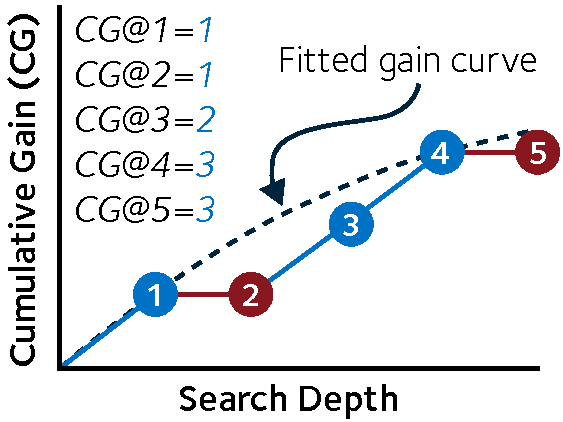
\includegraphics[width=1\textwidth]{figures/ch2-cg.pdf}
    \end{center}
    \vspace*{-4mm}
    \caption[Cumulative Gain]{An illustration of the~\glsfirst{acr:cg} as defined by~\cite{jarvelin2000cg, jarvelin2002cg}. In the example, the first five documents from a list are shown – 1, 3 and 4 contain information, from which the user gains information from. Also pictured is the fitted \emph{gain curve}.}
    \label{fig:cg}
\end{wrapfigure}

An important suite of measures that address these issues concern the notion of a searcher's \emph{gain} as he or she proceeds examines results. Put simply, as a searcher examines content for relevance, knowledge will be gained as he or she continues to do so. This gain is accumulated to produce the first measure,~\glsfirst{acr:cg}, as defined by~\cite{jarvelin2000cg, jarvelin2002cg}. Up to a given cutoff point $k$,~\gls{acr:cg} is measured as the cumulation of all relevance values for all documents up to rank $k$. A visual illustration of this is shown in Figure~\ref{fig:cg}. As used in prior experimentation,~\gls{acr:cg} has often been used in~\gls{acr:iir} simulation as the TREC assessor's document judgement values. For an example of this, refer to~\cite{maxwell2016agents}. Similar to~\gls{acr:cg} is the \emph{ranked half-life}, the point in a list of documents at where half of the total relevance of that set is achieved. Essentially, the ranked half-life is the formula for computing the median of a continuous set of data.

Considering the notion of positions within a list of results, a development to~\gls{acr:cg} is~\gls{acr:dcg}. Here, the gain obtained by a new document is discounted according to the rank of that document (i.e. \emph{weighted precision}). A new relevance score is therefore computed for each document by dividing the relevance score by the $log$ of its rank. These discounted scores are then summed, again to a similar cutoff value as described above. This provides an answer to the argument that a document at rank $55$ is less likely to be examined than a document at rank $5$. Even though both may contain relevant information, the perceived worth of the information contained in the document at rank $55$ is reduced to account for its depth in the results. Other measures that are inspired by~\gls{acr:cg} include \emph{Time-Biased Gain (TBG)}~\citep{smucker2012tbg}, a measure that aims to predict the distribution of the number of relevant documents a searcher will save when processing a list of results. 

\subsubsection{Rank-Biased Precision}
Considering on a similar vain to the notion of \emph{weighted precision models}~\gls{acr:rbp}~\citep{moffat2008rbp} is a more contemporary measure that is derived from a simple model of user behaviour. It considers the notion that searchers are not willing to examine every result presented to them. Illustrated in Figure~\ref{fig:rbp}, the underlying user model assumes that a searcher, when presented with a list of results, will always examine the first result, and will examine subsequent documents with a decreasing likelihood (probability $p$), called the \emph{patience} or \emph{persistence} parameter. The searcher's examination of a list will then end with probability $1-p$. Including the patience parameter allows for a very flexible measure to be defined. For example, one can model both persistent (where $p$ tends towards $1.0$) and impatient searchers (where $p\approx0.5$)~\citep{moffat2008rbp}. Indeed, with this flexibility, one can also model the \emph{I'm Feeling Lucky}\texttrademark~button on a Google search, with $p=0.0$ (equivalent to $P@1$).

\begin{figure}[t!]
    \centering
    \resizebox{1\hsize}{!}{
    \includegraphics{figures/ch2-rbp.pdf}}
    \caption[Rank-Biased Precision]{An illustration of the simple user model encoded within the~\gls{acr:rbp} measure. A user following this model will \emph{always} examine the first result presented, and will examine subsequent results with decreasing probability (from \emph{p}, the \emph{patience} or \emph{persistence} parameter). Stopping is determined with probability \emph{p-1}. Figure adapted, with permission, from~\cite{moffat2008rbp}.}
    \label{fig:rbp}
\end{figure}

Given a list of documents, $d$,~\gls{acr:rbp} is defined by~\cite{moffat2008rbp} as:

\begin{equation*}
RBP = (1 - p) \cdot \sum_{i=0}^{d}r_i \cdot p^{i-1}.
\end{equation*}

Above, $p$ denotes the patience parameter, with $r_i$ denoting the relevance judgement for a document at rank $i$.~\gls{acr:rbp} has been shown to fit well with actual user data extracted from click logs, as demonstrated in works by~\cite{chapelle2009rbp} and~\cite{zhang2010click_rbp}. Indeed,~\gls{acr:rbp} is used within this thesis as a means for attempting to decide when a simulated user is to stop. By incorporating an additional probability in conjunction with the calculated score at rank $i$, one can then determine, by incorporating some cutoff value $k$, whether a simulated user should stop or continue. Given the success that~\gls{acr:rbp} has had in the literature over the past decade since it was first derived, such a stopping model would be expected to yield good approximations of actual searcher stopping behaviour.

\subsubsection{INST}
The final measure that we consider is the more recently defined \emph{INST} measure, as described by~\cite{bailey2015inst, moffat2015inst}. INST considers the \emph{conditional probability} that a searcher, having examined a document at rank $i$, will examine the next document, at rank $i+1$.


\section{Chapter Summary}
In this chapter, we have introduced some of the key constructs of traditional~\gls{acr:ir}: from indexing documents, to retrieval models, to the ways in which such systems are evaluated. We have also briefly touched on the history of the field, examining some of the manually operated systems that we can today regard as an~\gls{acr:ir} system.

With the focus of this thesis very much on the interactions of users with~\gls{acr:ir} systems, we then turned our attention to the study of~\gls{acr:iir}, detailing a variety of different types of study that can be undertaken in the area. Specifically, we have looked at the basic, underlying user model that are encoded within the Cranfield model (Figure~\ref{fig:trec_model}), and have examined a number of different evaluation measures to help us understand how well users perform. Considering the strong assumptions that the underlying user model poses, the following chapter discusses some of the more complex user models that have been subsequently published in the literature that attempt to carefully deconstruct these assumptions to produce more advanced, realistic means of encapsulating the various processes that take place between a user and system during search.


% Basic concepts -- given a query, tries to satisfy that query.
% Follows a system-orientated methodology
%
% From Leif:
% - indexing
%     tokenizers, etc
% - retrieval models
%     - these models have some notion of how much someone should retrieve/stop.
%     - boolean, look at whole set of documents
%     - other models, there's a cutoff... e.g. cosine similarity, angle gets too large, so you stop.
%     - probabilistic ranking principle
%
%         \begin{quote}
%             ``If a reference retrieval system's response to each request is a ranking of the documents in the collections in order of decreasing probability of usefulness to the user who submitted the request, where the probabilities are estimated as accurately as possible on the basis of whatever data has been made available to the system for this purpose, then the overall effectiveness of the system to its users will be the best that is obtainable on the basis of that data.''
%             \attrib{W.S. Cooper, in private correspondence to~\cite{robertson1977prp}.}
%         \end{quote}
%
%
%         - decreasing probbaility of relevance
%         - get odds of rel over non-rels, so there is some idea of a cut-off.
%         - why would you look at a document that is less relevant?
%         - nobody uses it, just make this observation.
% - evaluation
%     - effects of pooling in judgements?
%     - system orientated (cranfield)
%         - precision
%         - recall
%     - user orientated
%
%     - diane kelly's spectrum of system to user orientated
%         - TREC/Cranfield is a very basic approach to simulation
%             a model of how user performs
%         - user orientated approach looks at how users interact with the system
%         - models of how users search... to show how we develop models.
%
%         - at the end of chapter



% how do people actually interact with a ranked list?
% when do they stop, for example?
%
% we can employ a hybrid approach of conducting user studies to develop a more advanced, TREC++ user model of search.
%
% this model is guided and informed by actual user studies (as discussed in chapters x, y and z).
%
% and then we can test these models out to see whether they are any good by simulating a more advance user, with weaker assumptions, thus moving the area of user modelling forward.







% \subsection{Simulating the User}\label{sec:ir_background:user:simulation}
%
%
% For the purposes of this thesis, we focus upon the studies delineated by categories x and y.
%
%
% central to all of this is the user.
% talk about diane's spectrum of IR experimentation, from system to user focused.
% consider a variety of more user-centric evaluation approaches.
% here, you can also bring in the notion of simulation
% mention that this is IIR.
%
%     - diane kelly's spectrum of system to user orientated
%         - TREC/Cranfield is a very basic approach to simulation
%             a model of how user performs
%         - user orientated approach looks at how users interact with the system
%         - models of how users search... to show how we develop models.
%
%         - at the end of chapter
%
% Look at Kelly (2009) -- Methods for Evaluating Interactive Information Retrieval Systems with Users
%
% these measures/evaluations are thining about the way people go and search
% of relevance to this thesis are stopping strats
% diff. measures encoe different stopping models. different ways of evaluating this.
% in the next chapter, provide an overview of the different types of models of search, and how searching has been conceptualised with respect to stopping strategies.
%
%
%
% \subsection{TREC Ad-Hoc}\label{sec:ir_background:user:trec}
% \todo{does this bit need to be moved to the next chapter?}
% - searcher acquires an information need, sits down, and conducts a search against an existing collection of documents over a set period of time. Known as ad-hoc retrieval, or retrospective searching in older literature.
%
% - this is lifted from Robertson (2008), rephrasing required, and probably needs to be moved to the user model part.
%
% - The user model invoked here is what has now become the most obvious one for search: user has an
% information need, sits down in front of a system and conducts a search against an existing collection of
% documents, over a limited time period. This is known in TREC jargon as an ‘ad-hoc’ search – an earlier more-orless
% equivalent term was ‘retrospective searching’. System produces a ranked list of items, which the user consults
% in rank order. Users may judge documents good or bad, but in principle there may be any number of good
% documents in the collection. (The one significant change in this model from the Cranfield view is that there is now
% an assumption that each system will rank its results list.) It is often asserted that there is also an assumption that
% requests are topical or subject-based (documents about X); indeed the TREC jargon, which is to call requests
% ‘topics’, encourages that view18. However, although most of the requests used in TREC (all of those in early
% TRECs) are indeed topical, there is no necessary requirement of the model that this should be so, or that they
% should be purely topical. In some sense the nature of the requests is determined by the relevance judgements; if
% the judgements depend on other criteria than pure topicality, then that is the nature of the task.
% However, it is fundamental to the model that the judge or assessor should indeed be able to make a judgement
% on each document, actually a binary one for most of the TREC ad-hoc tasks, and should be able to make the
% judgement irrespective of the order of presentation of the documents. This last precludes, for example, embedding
% a criterion of novelty in the usual ad-hoc task relevance judgements (although one track did investigate novelty by
% making judgements of novelty separated from the relevance judgements). A typical TREC ‘topic’ has a short title (which might be used directly as a query), and additional information about the
% supposed information need under the headings ‘description’ and ‘narrative’. The narrative contains explicit rules for
% judging the relevance of documents. An example title and description are: Hydroponics—Document will discuss the
% science of growing plants in water or some substance other than soil.
    % %!TEX TS-program = xelatex
%!TEX root = ../../maxwell2018thesis.tex

\chapter[Searching and Stopping]{Searching and Stopping:\\A Background}
\label{chap:stopping}
Having established the main focus of this thesis, this chapter provides a detailed overview of the current state of the literature in the context of stopping during search, and the varying ways in which it has been examined and subsequently modelled. We examine this from two main perspectives, considering:

\begin{itemize}
    \item{the \textbf{conceptual and descriptive} approaches that have been undertaken; and}
    \item{the \textbf{formalised} approaches that have been examined.}
\end{itemize}

Conceptual and descriptive approaches generally consider a high-level approach of stopping. Approaches taken, as described in this chapter, include a series of \emph{stopping heuristics and rules} (Section~\ref{sec:stopping:heuristics}) and a series of user studies examining the phenomenon and the wider \emph{Information Seeking and Retrieval (ISR)} process~\citep{kelly2013evaluation_review}, as detailed in Section~\ref{sec:stopping:studies}. These approaches generally provide a picture of the domain, with this information subsequently allowing us to develop more formalised approaches~\citep{azzopardi2015theories}.

In turn, formalised approaches are more precise, building upon the knowledge and understanding obtained from the conceptual and descriptive approaches. Generally, a formalised approach enumerates each aspect of the phenomena as a variable, allowing one to explore how varying each variable functionally relates to others. In the context of examining one's stopping behaviour, a number of different formalised ISR models have been proposed, which we discuss in relation to stopping in Section~\ref{sec:stopping:theories}.

\section{User Studies}\label{sec:stopping:studies}
what have studies shown that examine stopping behaviour?

~\cite{wu2014information_scent}\\
~\cite{dostert2009satisficing}\\
~\cite{toms2009predicting_stopping}\\
~\cite{zach2005enough_is_enough}\\
~\cite{wu2014stopping_query_abandonment}\\
~\cite{marchionini1995information_seeking}


\section{Stopping Heuristics}\label{sec:stopping:heuristics}
Despite the inherent difficulties that have been observed when ascertaining how and when people stop searching, researchers have over the years proposed a number of different stopping heuristics which are \emph{believed} to provide a more concrete means of quantifying and/or explaining when searchers decide to stop, and thus quantifying the sense of what is \emph{``good enough''}~\citep{wu2014information_scent}.

A majority of these heuristics can be found within~\gls{ir} research, with the earliest having been defined as far back as the early 1970's. These heuristics are generally high level, \emph{conceptual} approaches that describe when searching should stop, at different levels (e.g. the session level, or the query level). To describe each of the heuristics, we break this section up into a number of different subsections, which provides a loose classification of the different approaches that have been described in the literature. We consider first:

\begin{itemize}
    
    \item{a \emph{fixed-depth} approach, considered as the de facto stopping heuristic used in much~\gls{ir} research today.}
    
\end{itemize}

From this, a series of more \emph{adaptive} heuristics are defined in the literature which we consider in turn. These are:

\begin{itemize}
    \item{tolerance to non-relevance;}
    \item{satiation rules;}
    \item{difference rules;}
    \item{time-based rules; and}
    \item{patch-based rules.}
\end{itemize}

\subsection{The Fixed Depth}
Preciaion-at-k is the classic example here.
You will go to a fixed depth always
Assumed by the cranfield paradigm, for example.

unrealistic. so what other approaches are there in the literature?
a number of different rules are explained in the literature.

\subsection{Cognitive Heuristics}
By far the largest category of stopping heuristics defined within the literature are \emph{cognitive based} heuristics. That is to say, heuristics that attempt to model in some form of criterion or criteria that are met in the mind of the searcher as he or she examines content to determine what is and what is not relevant.

\subsubsection{Tolerance to Non-Relevance}



\citeauthor{cooper1973retrieval_effectiveness} worked on two studies~\citep{cooper1973retrieval_effectiveness, cooper1973retrieval_effectiveness_ii} that argued that the best way in which to evaluate a retrieval system would be to elicit subjective estimates of the system's utility to its users.



It was argued in Part I (see JASIS, March-April 1973 p. 87) that the best way to evaluate a retrieval system is, in principle at least, to elicit subjective estimates of the system's utility to its users, quantified in terms of the numbers of utiles (e.g. dollars) they would have been willing to give up in exchange for the privilege of using the system; and a naive methodology was outlined for evaluating retrieval systems on this basis. But the impracticality of the naive evaluation procedure as it stands raises the questions: How can one decide which practical measure is likely to yield results most closely resembling those of the naive methodology? And how can one tell whether the resemblance is close enough to make applying the measure worth while? In the present paper two kinds of solution to these problems are taken up. The first answers the questions in terms of the reasonableness of the simplifying assumptions needed to get from the naive measure to the proposed substitute. The second answers it by experimentation.


~\cite{cooper1973retrieval_effectiveness}

~\cite{cooper1973retrieval_effectiveness_ii}


cooper.
pretty much the same rule was defined by nickles

considers a searcher's tolerance to non-relevance.


\subsubsection{Satiation Rules}

\subsubsection{Difference}

\subsubsection{The Mental List}

\subsubsection{Representational Stability}

\subsubsection{Magnitude Threshold}

\subsubsection{The Single Criterion}

\subsection{Time-Based}

\subsection{Patch Rules}

\section{Formal Theories of Interaction}\label{sec:stopping:theories}
Understanding the complex behaviours exhibited by searchers during the ISR process has been a longstanding problem~\citep{azzopardi2015theories}. With most approaches considering the direct observation of searcher behaviours through interaction log data as described previously in Section~\ref{sec:stopping:studies}, several attempts have been made to provide mathematically grounded, formalised theories that describe this process. From these theories, one can then begin to deduce a series of testable hypotheses when undertaking interaction studies, such as the hypothesis provided in Chapter~\ref{chap:snippets}, and as published in~\cite{maxwell2017snippets}.

We discuss in this section three main competing ISR theories, all of which provide a rational explanation of \emph{when searchers should stop}.

\begin{itemize}
    \item{\textbf{\emph{Information Foraging Theory (IFT)}}~\citep{pirolli1999ift}, which considers a searcher \emph{foraging} for information to be analogous to an animal foraging for food in the wild -- allowing for the inclusion of many theoretical approaches used in ecology to be applied to search (Section~\ref{sec:stopping:theories:ift});}
    
    \item{the \textbf{\emph{Interactive Probability Ranking Principle (iPRP)}}~\citep{fuhr2008iprp}, allowing for the modelling of a searcher in making decisions, or \emph{choices}, during an interactive search session (Section~\ref{sec:stopping:theories:iprp}); and}
    
    \item{\textbf{\emph{Search Economic Theory (SET)}}~\citep{azzopardi2011economics}, where the search interactions that take place between a searcher and the computer is modelled as an economics problem (Section~\ref{sec:stopping:theories:set}).}
\end{itemize}

Paradoxically, an astute way in which to introduce these formal models is to begin by discussing a \emph{conceptual model} -- the \emph{Berry Picking Model}.

\begin{figure}[t!]
    \centering
    \resizebox{1\hsize}{!}{
    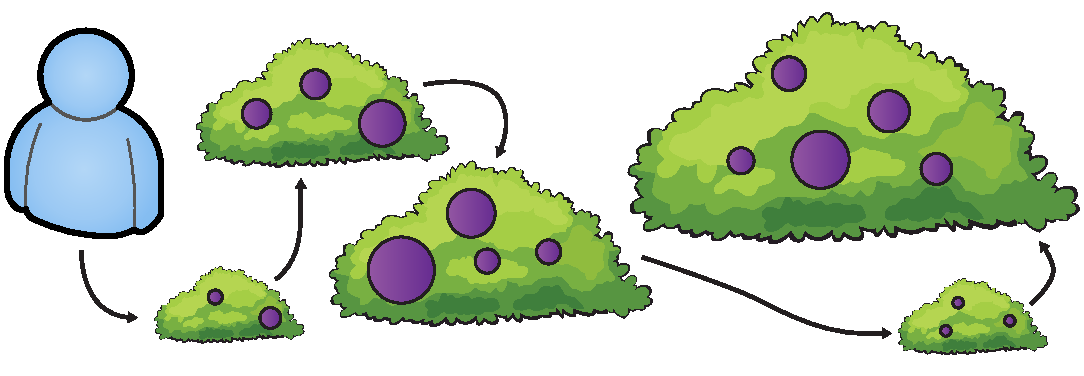
\includegraphics{figures/ch3-berry_picking.pdf}}
    \caption[Berry Picking]{A crude illustration depicting \emph{Bates' Berry Picking model}~\citep{bates1989berry_picking}. In this conceptual model, a berry picker forages through a series of \emph{patches} (refer to Section~\ref{sec:stopping:theories:ift} for more information; patches are represented in the illustration as bushes) in search of the ripest berries (a simple assumption would be to assume larger berries are riper). This model mirrors how an individual searches with an evolving information need.}
    \label{fig:ch3-berry_picking}
\end{figure}

\subsection{From Conceptual to Formal}\label{sec:stopping:theories:conceptual}
As illustrated in Figure~\ref{fig:ch3-berry_picking}, the Berry Picking Model~\citep{bates1989berry_picking} draws an analogy between a searcher and a \emph{forager} -- in this case, a forager looking for berries. The forager attempts to collect the ripest berries within a series of different \emph{patches} (refer to Section~\ref{sec:stopping:theories:ift} for more information on the \emph{patch model}). This is crudely illustrated in Figure~\ref{fig:ch3-berry_picking}, where the forager moves between bushes (patches). Once the ripe berries have been collected from a patch, the forager moves to the next patch, until all patches have been exhausted. The analogy here regarding search considers a patch as a SERP, with a forager here attempting to look for the most relevant documents to their information need. As stated by~\citeauthor{bates1989berry_picking}, the forager's information need evolves, and so the type of information they attempt to find valuable at a given point also changes. Switching back to the berry picking analogy, this may mean a switch between blueberries and strawberries, for example.

While this conceptual model is intuitive and subsequently easy to understand, the model lacks the ability to describe how long a forager will spend in an individual patch, or how long the time taken to reach a patch in the first place will affect their behaviour~\citep{azzopardi2015theories}. The lack of explanation is where more formalised approaches attempt to provide an answer. For example, researchers took forward the concept of a searcher as a forager (e.g.~\cite{russell1993sense_making, sandstrom1994optimal_foraging}), with their results suggesting that \emph{Optimal Foraging Theory (OFT)}~\citep{stephens1986foraging_theory} could be used to model the search process. This subsequently gave rise to the theory of Information Foraging Theory~\citep{pirolli1999ift}.

\subsection{Information Foraging Theory}\label{sec:stopping:theories:ift}
Analogous to an organism foraging for food in the wild, Information Foraging Theory considers a searcher as an \emph{informavore}\footnote{The term \emph{informavore} was originally coined by~\citeauthor{miller1983informavores}. \emph{``Just as the body survives by ingesting negative entropy, so the mind survives by ingesting information. In a very general sense, all higher organisms are informavores.''}}, an organism that consumes \emph{information.} IFT is comprised of a \emph{ternion} of underlying models~\cite{pirolli1999ift}, which are explained below. A graphical illustration of the three models can also be seen in Figure~\ref{fig:ch3-patch}.

\begin{figure}[t!]
    \centering
    \resizebox{1\hsize}{!}{
    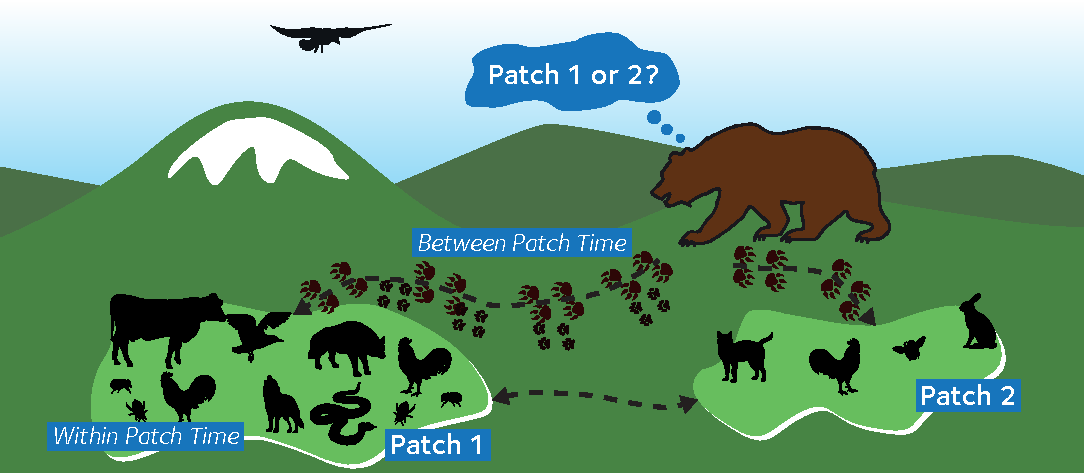
\includegraphics{figures/ch3-patch.pdf}}
    \caption[Illustration of the Patch Model]{A graphical representation of various models that form Information Foraging Theory. Should the forager expend effort navigating to \emph{Patch 1}, or \emph{Patch 2}? \emph{Patch 1} is further away, with a stronger scent, and offers more potential gain (food). However, \emph{Patch 2} is closer. IFT provides a framework for addressing these issues. Also shown within the illustration are the \emph{between patch} and \emph{within patch} times that are spent by the forager. Refer to Section~\ref{sec:stopping:theories:ift} for an explanation on what these times represent. Silhouettes acquired from \emph{freepik.com}.}
    \label{fig:ch3-patch}
\end{figure}

\begin{itemize}
    
    \item{The \textbf{\emph{Information Scent model}} considers how informavores rely upon various \emph{proximal cues}~\citep{chi2001information_scent} (e.g. bolded terms, other textual snippets, or graphics within \emph{information cards} -- see~\cite{bota2016information_cards}, for example) to indicate how promising a particular patch (e.g. a document) looks to be in terms of satisfying their information need. This is analogous to an organism foraging for food; organisms rely upon various cues in the surrounding environment (e.g. paw prints, smells) to guide them to a promising patch. Both informavores and herbivores/carnivores estimate how beneficial following a particular path, or \emph{scent trail}, will be\footnote{A discussion of this explanation can be found by Jakob Nielsen at \url{https://www.nngroup.com/articles/information-scent/} -- last accessed December 7\textsuperscript{th}, 2017.}. Once the scent starts to weaken (i.e. when no more additional information is expected to be found), a informavore will stop and progress to a different scent trail~\citep{piorkowski2012information_scent}.}
    
    \item{The \textbf{\emph{Information Diet model}} -- when considering a webpage as a patch and information as the prey -- provides a rationale for determining which information a forager will consume. Leaving a particular website may be straightforward, but finding a better one is not necessarily so -- although it can be argued that in recent years, the advancement of search engine technology has made this issue to be less of a challenge~\citep{vaughan2004new_measurements}. If it for example is easier for a forager to find lots of potentially useful webpages, there is less incentive for them to stay on a single page; technological developments today encourage the consumption of small chunks of information from a high number of sources, and, as such, a change in our behavioural characteristics.\footnote{The idea of technology changing our behavioural characteristics is not new; an article in the \emph{New York Times} suggests that the development of technology has made us more impatient, expecting instant answers -- and more forgetful, too, in the sense that the relative cost of accessing information is now so low, we readily discard information. The article is available at \url{http://www.nytimes.com/2010/06/07/technology/07brainside.html}, last accessed December 7\textsuperscript{th}, 2017. Refer also to~\cite{carr2008google_stupid}.}}
    
    \item{Finally, \textbf{\emph{Information Patch model}} concerns how long a forager will stay in a particular \emph{patch} (e.g. an area of land, or, in terms of an informavore, a list of ranked documents, for example) before deciding to move to a new patch.}
    
\end{itemize}

We consider the Information Patch model as of particular relevance to the work in this thesis, as it concerns when a forager will \emph{stop} examining a given patch. Given the illustration in Figure~\ref{fig:ch3-ift}, the analogy for an information seeker -- or informavore -- is that:

\begin{itemize}
    \item{\emph{moving between a patch} is like \emph{issuing a new query}, and the subsequent query formulation cost that must be expended; and}
    \item{\emph{staying within a patch} is analogous to \emph{assessing a series of documents}, where each document incurs an examination cost.}
\end{itemize}

With these assumptions in hand, the Information Patch model allows for the prediction of how long a forager should stay in a patch before moving to the next patch. As IFT is based upon Optimal Foraging Theory (OFT)~\citep{stephens1986foraging_theory}, two main assumptions about the forager are made, in that, unsurprisingly, they will act in an optimal fashion:

\begin{itemize}
    \item{the forager will \emph{always enter the patch with the highest potential yield first}; and}
    \item{the forager will \emph{maximise their gain per unit of time} spent in a patch~\citep{pirolli1999ift, stephens1986foraging_theory}.}
\end{itemize}

When considering the sample illustration in Figure~\ref{fig:ch3-patch}, this therefore means that the forager will enter \emph{Patch 1} first, as this patch offers the largest return for the energy the forager initially expends reaching the patch. When considering the stopping behaviour exhibited by a forager, one needs to calculate the gain attained at a given point in time, or $g(t)$. From this, the moment at which a forager should optimally stop examining a patch is the point in time at which the maximal value of gain per unit of time is reached. This is dependent upon a number of factors, including aspects such as the \emph{between patch} and \emph{within patch} times -- the times spent getting to a patch, and spent within a patch, examining content, respectively. 

Figure~\ref{fig:ch3-ift} provides two plots to demonstrate the theory in action, demonstrating on the left a gain. The illustration shows four gain curves that are for individual patches, each under different conditions. We show the difference in stopping times between patches with both a low and high between-patch time (i.e. a longer time to enter the patch from zero time), and patches which are fruitful, giving a high yield, and those with a low yield. By taking the gain curves and drawing the tangent to the curve through the origin, we can then see that the optimal stopping point as dictated by IFT is the point on the gain curve where its tangent intersects with it. This is the point of the \emph{maximal rate of gain}; foragers spending time within the given patch after this point will experience continually diminishing returns. IFT suggests that after this point, a forager should abandon the patch, and then proceed to issue a new query, and subsequently enter a new patch.

\begin{figure}[t!]
    \centering
    \resizebox{1\hsize}{!}{
    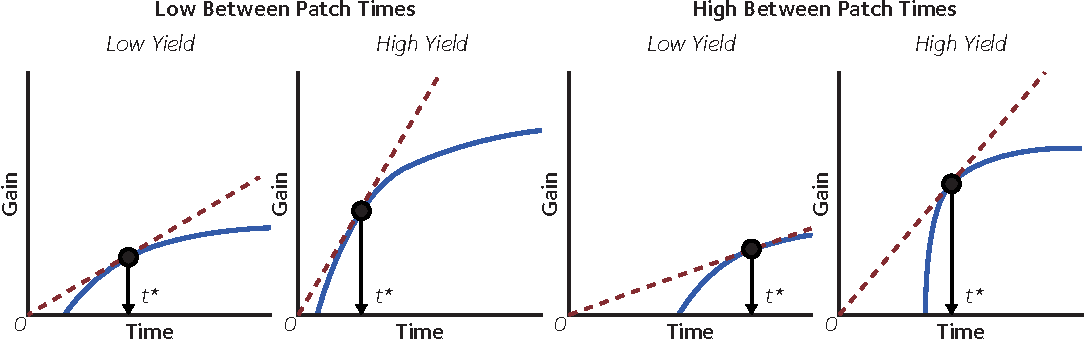
\includegraphics{figures/ch3-ift.pdf}}
    \caption[Plots of optimal patch stopping points for Information Foraging Theory]{Four plots, each denoting a different scenario for the optimal stopping point within a patch, as outlined by \emph{Information Foraging Theory}. The two plots on the left denote a low between-patch time, with the two right plots illustrating a high between patch time. The \emph{Low Yield} plots denote smaller levels of gain per unit of time compared to the \emph{High Yield} patches. Note the optimal stopping point is denoted by \emph{t*}, the point at which the tangent of the gain curve intersects. Time spent within the patch after this point will result in steadily diminishing returns.}
    \label{fig:ch3-ift}
\end{figure}

\vspace{-5mm}
\subsection{Considering Costs and Benefits}
The other means by which information seeking has been formally modelled is through the consideration of the \emph{costs} and \emph{benefits} that a searcher must consider during the search process. Although not discussed in the original Berry Picking model,~\citeauthor{bates1979search_tactics} does discuss the idea that these should be weighed up in subsequent work~\citep{bates1979search_tactics}.

The idea of using a cost/benefit analysis is not new; a number of other formal models have been created using this underlying approach. In~\gls{ir} research for example, purchasing decisions and ranking have been considered using this approach. A more user-centric approach was undertaken by Cooper, who modelled the trade-off between how long a searcher should spend searching, and how much time the system should itself spend searching. More related to the work in this thesis is the \emph{Probability Ranking Principle (PRP)} by~\citeauthor{robertson1977prp}, who proposed a formalised model utilising decision theory to the so-called \emph{ranking problem}~\citep{robertson1977prp}. The PRP essentially formed a theoretical foundation for optimising the results of ad-hoc retrieval. The PRP itself has in past decade been extended to yield the \emph{Interactive Probability Ranking Principle}~\citep{fuhr2008iprp}, as discussed in Section~\ref{sec:stopping:theories:iprp} below.

\subsubsection{The Interactive Probability Ranking Principle}\label{sec:stopping:theories:iprp}
With the PRP considering only the ranking problem, the notion of user interactions during ad-hoc retrieval are largely ignored by this theory. Systems have been shown in previous studies to perform differently in in a standard retrieval setting, of a single query and ad-hoc retrieval (e.g.~\cite{voorhees2000trec8, turpin2006performance_versus_measures}). Using the PRP, this approach is indistinguishable from an interactive setting. Studies have also shown that scanning through a list of ranked documents to identify potentially relevant entries may not be the most crucial activity in the~\gls{iir} process~\citep{turpin2001batch_evaluations}. As such. the iPRP provides and extension to the classical PRP, providing a means of formalising various activities within a search session besides simply scanning a ranked list of results.

Based upon the preexisting PRP, the iPRP removes two key assumptions that the PRP makes to increase the flexibility of the underlying model. These changes include the removal of the assumptions that consider:

\begin{itemize}
    \item{a \emph{fixed information need}, allowing a user modelled by the iPRP to have an information need that changes and adapts as documents are examined (e.g. as per the \emph{Anomalous State of Knowledge (ASK)}, described by~\citeauthor{belkin1980ask}); and}
    \item{the assumption that the \emph{relevance of documents is independent of other documents}.}
\end{itemize}

While sensible assumptions to make for the purposes of modelling, it has been demonstrated that the assumptions do under certain circumstances break down~\citep{gordon1991utility_theory}. From these updated assumptions, three main requirements were specified, namely that iPRP must:

\begin{enumerate}
    \item{consider the interaction process as a whole, rather than simply considering document ranking as was assumed in the classical PRP;}
    \item{allow for different of costs and benefits to be invested and given respectively, meaning that, for example, a longer document will take a greater period of time to examine than a shorter document; and}
    \item{allow for the changing of the information need throughout the course of the search session, \`{a} la~\cite{belkin1980ask}.}
\end{enumerate}

This last point is reminiscent of Bates' Berry Picking model. As outlined in Section~\ref{sec:stopping:theories:conceptual}, a forager would traverse through patches/bushes in order to find the ripest berries available. However, as they forage, they may find, for example, certain berries to be riper than others. As such, they adjust what they are foraging for as they acquire more berries. In terms of an information seeker, this is analogous of a searcher's mental model of a particular topic continually evolving as they are subjected to new information through each document they examine. As such, one's information need may change as new information is uncovered.

From these requirements, the iPRP was then created with four revised assumptions, namely that:

\begin{enumerate}
    \item{there should be a focus on the function level of interaction, meaning that there are a variety of different activities one can undertake (e.g. query formulation, document examination), with each activity having a cost and benefit associated with it;}
    \item{\emph{decisions} forming the basis of interaction;}
    \item{the searcher evaluating the \emph{choices} laid before him/her in a \emph{linear order} (i.e. when examining a list of ranked results, starting from the top and working your way down); and}
    \item{only decisions that are positive and correct are of benefit to the searcher.}
\end{enumerate}

\subsubsection{Search Economic Theory}\label{sec:stopping:theories:set}
The origins of SET can be traced back to work by~\cite{varian1999economics}, who outlined three directions in which 

\section{Chapter Summary}

\begin{itemize}
\item there has been lots of conceptual work on trying to understand stopping behaviours, but most boil down to the fact that people stop because what they have found is “good enough”.
\item despite this, we have all these different heuristics that researchers define — primarilry mental rule that searchers tick off as they go through results. And once a criterion/some criteria have been satisfied, they stop.
\item and now we have theories of information seeking behaviour which also provide us with a mathematical means for trying to deduce when people stop. These are themselves stopping rules.
\item this goes back to what I am saying in chapter 2, which states that most models and measures that we use all encode within them some form of stopping model — they are just not particularly realistic.
\item and from here, we can go: we have these heuristics and rules, but there is nothing in the literature to show how well these rules perform when compared to real behaviours. We know that behaviours change under different search contexts; it therefore follows that stopping behaviour will also change. And so, in order to look at this, we now introduce our conceptual search model (next chapter), before using this model in a series of simulations to ascertain exactly how stopping behaviour changes under different conditions/different search goals (remaining chapters).
\end{itemize}

    %
    %!TEX TS-program = xelatex
%!TEX root = ../../maxwell2018thesis.tex

\part[Advancing User Modelling]{In this part of the thesis, we introduce the \darkbluebox{Complex Searcher Model (CSM)}. The CSM provides a more complex and realistic conceptual model of the~\gls{acr:iir} process. Embedded within the CSM is a new \darkbluebox{stopping decision point} – this is analysed in detail, allowing us to determine whether it enjoys better approximations of actual searcher behaviours.}{Advancing User\\Modelling in~\gls{acr:iir}}\label{part:stopping}
    % %!TEX TS-program = xelatex
%!TEX root = ../../maxwell2018thesis.tex

\chapter[Advancing User Modelling in IIR]{Advancing User Modelling in IIR}

``Empirical studies of complete systems mostly focus on variations of single components''~\citep{fuhr2008iprp}

In previous chapter we have seen a number of different entire search session models.
In this chapter, we introduce a number of models that have been considered throughout this PhD, with a focus on stopping decision points.

- Why do we consider this as a flow chart?
It's a high-level, conceptual model, where different states/activities are represented as components.
Totally up to how one implements each component -- i.e. with stopping components, we can instantiate them in a number of different ways.

- these models are based on stochastic approaches.


\section{The Basic User Model}
Query, Document, Mark

\section{The Complex Searcher Model}
introduce the model, explaining and motivating it

\subsection{CSM, Mark I}
Query, Snippet, Document, Mark

\subsection{CSM, Mark II}
- motivation for including the SERP
- Query, SERP, Snippet, Document, Mark
- ECIR 2018 paper

\subsection{Considering State and Agency}
- as an aside, we can also incorporate state and agency into the model.
- to a degree, the mark I and mark II models already do consider some form of state, by virtue of having a record of what documents have been previously examined, for example.
- however, we can go further here, introducing more advanced state, leading to some form of agency. for example, an agent can determine a new set of queries based upon what it has previously observed.

- while not central to the thesis, we can at least consider it, and demonstrate that it is indeed useful.


\section{Evaluating Model Effectiveness}
Core to developing a new model is to basically improve our representation of a real world phenomenon, such as, in this case, the search process.

\subsection{Research Questions}
Allowing us to address HL-RQ1.

\subsection{Experimental Design}

\subsection{Results}

% \section{Introduction}
% \section{Components of the Model}
% \section{Evolution of the Model}
% \section{Incorporating State and Agency}
% \subsection{Section Introduction}
% \subsection{Research Questions}
% \subsection{Experimental Design}
% query reformulation is a good contribution here. the agent is able to generate queries based upon what it has seen.
% \subsection{Results}
% \subsection{Discussion and Conclusions}
% \section{Chapter Summary}
    % %!TEX TS-program = xelatex
%!TEX root = ../../maxwell2018thesis.tex

\chapter[Operationalised Stopping Strategies]{Operationalised\\Stopping Strategies}\label{chap:strategies}
In Section~\ref{sec:stopping_background:heuristics}, we discussed a number of different \emph{stopping heuristics} that have been previously defined in the literature. A majority of these heuristics were derived from the concept of \emph{satiation}~\citep{simon1955satiation} -- that is, the searcher abandons their search when they feel satisfied with what they have found. These heuristics were conceptual in nature, being derived from a number of underlying theories and assumptions.

In this section, we take a number of these stopping heuristics forward to produce a series of different~\glsplural{glos:stopping_strategy}, providing an answer that addresses \blueboxbold{HL-RQ2}.\footnote{Refer to Section~\ref{sec:intro:rqs} on page~\pageref{sec:intro:rqs} for the definition of the research question.} These strategies are operationalised versions of the corresponding heuristics. This means that we can subsequently implement and test them, with explanations as to how we tested them provided in our general methodology, in Section~\ref{chap:csm:method:simulation:grounding:stopping_strats}. The stopping strategies are enumerated over seven categories, which are:

\begin{itemize}
    \item{our baseline, the \blueboxbold{fixed depth} stopping strategy;}
    \item{stopping strategies considering the searcher's tolerance to \blueboxbold{frustration};}
    \item{a \blueboxbold{satisfaction} based stopping strategy;}
    \item{stopping strategies based upon the \blueboxbold{difference} threshold stopping heuristic;}
    \item{a strategy based upon~\blueboxbold{\gls{acr:ift}};}
    \item{a series of \blueboxbold{time-based} stopping strategies; and}
    \item{two stopping strategies based upon established~\gls{acr:ir} evaluation measures.}
\end{itemize}

Although each of these~\glsplural{glos:stopping_strategy} could in theory be applied to any of the three stopping decision points summarised in Section~\ref{sec:csm:csm:stopping}, we consider them only from a snippet level in this thesis. This does not mean to say we do not explore the additional two stopping decision points -- Chapter~\ref{chap:serp} explores the~\gls{acr:serp} level stopping decision point, and Chapter~\ref{chap:diversity} examines the effect of the session level stopping decision point on stopping behaviour.

In addition to this, we do not consider all of the various stopping heuristics (outlined in Section~\ref{sec:stopping_background:heuristics}) in this chapter. This is for a variety of factors, the chief of which is that many of the more complex stopping heuristics are difficult to model, when one has to consider the cognitive processes involved. For example, the mental list stopping heuristic (Section~\ref{sec:stopping_background:heuristics:reasoning:list}) appears to be more topic specific, requiring a searcher to know \emph{a priori} all the criteria that they need to check off in their head. However, these criteria are largely unknown in ad-hoc circumstances.

In the remainder of this chapter, we consider each of the categories enumerated above in turn, discussing the different operationalised stopping stopping strategies that we consider for the empirical work in this thesis.

\blueboxheader{A Note on Notation}
Each of the operationalised stopping strategies that are introduced in this chapter come complete with \emph{stopping threshold} variables, allowing one to customise the point at which the searcher would stop when employing such a strategy. As demonstrated in the front matter of this thesis, the notation we use to illustrate a stopping strategy and its stopping threshold variable is \stoppingstratbox{SS1-FIX}{3} -- this example denotes stopping strategy \stoppingstratboxsingular{SS1-FIX}, with a stopping threshold of $3$.\footnote{Refer to Section~\ref{chap:strategies:fixed} for information on this particular stopping strategy.}

%\noindent\blueboxbold{A Note on Usefulness} In this section, we refer to the concept of a result summary being \emph{useful} and \emph{unhelpful}. By this, we mean that a summary appears to be of use for a searcher to satisfy his or her information need. In the context of simulation, this notion of relevance does not necessarily correspond to the judgement made in a gold standard that is being compared to: the notion of usefulness in this context represents the decisions that are taken by a searcher as to what constitutes a useful or unhelpful document/result summary.

\section{Fixed Depth}\label{chap:strategies:fixed}
The fixed depth stopping strategy is based upon an assumption held across many of the models and measures that are widely used throughout the~\gls{acr:ir} community. The assumption is that a searcher, when examining a list of ranked results for their query, will browse to a \emph{fixed depth} in the rankings before stopping -- the roots of which can be traced back to the Cranfield paradigm as discussed in Section~\ref{sec:ir_background:basics:cranfield}. Examples of use include the basic stopping model implicitly encoded within measures such as~\gls{acr:patk}. The fixed depth assumption is also widely used in the simulation of interaction. For example,~\cite{azzopardi2011economics} conducted a large-scale simulated analysis, where simulated users examined content to depths ranging from $5$ to $1,000$ ($1,000$ is typically assumed in~\gls{acr:trec} style experimentation, where a single query is issued). Given the wide use of this fixed depth approach in historical and contemporary~\gls{acr:ir} research, we consider this stopping strategy as the baseline approach to which we will be comparing the more advanced, \emph{adaptive} stopping strategies.

\begin{itemize}
    
    \item{\blueboxbold{SS1-FIX}} A searcher employing this stopping strategy will stop searching once they have observed $x_1$ result summaries (i.e. \stoppingstratbox{SS1-FIX}{x1}), regardless of the relevancy of each judged result summary.
    
\end{itemize}

\begin{figure}[t!]
    \centering
    \resizebox{1\hsize}{!}{
    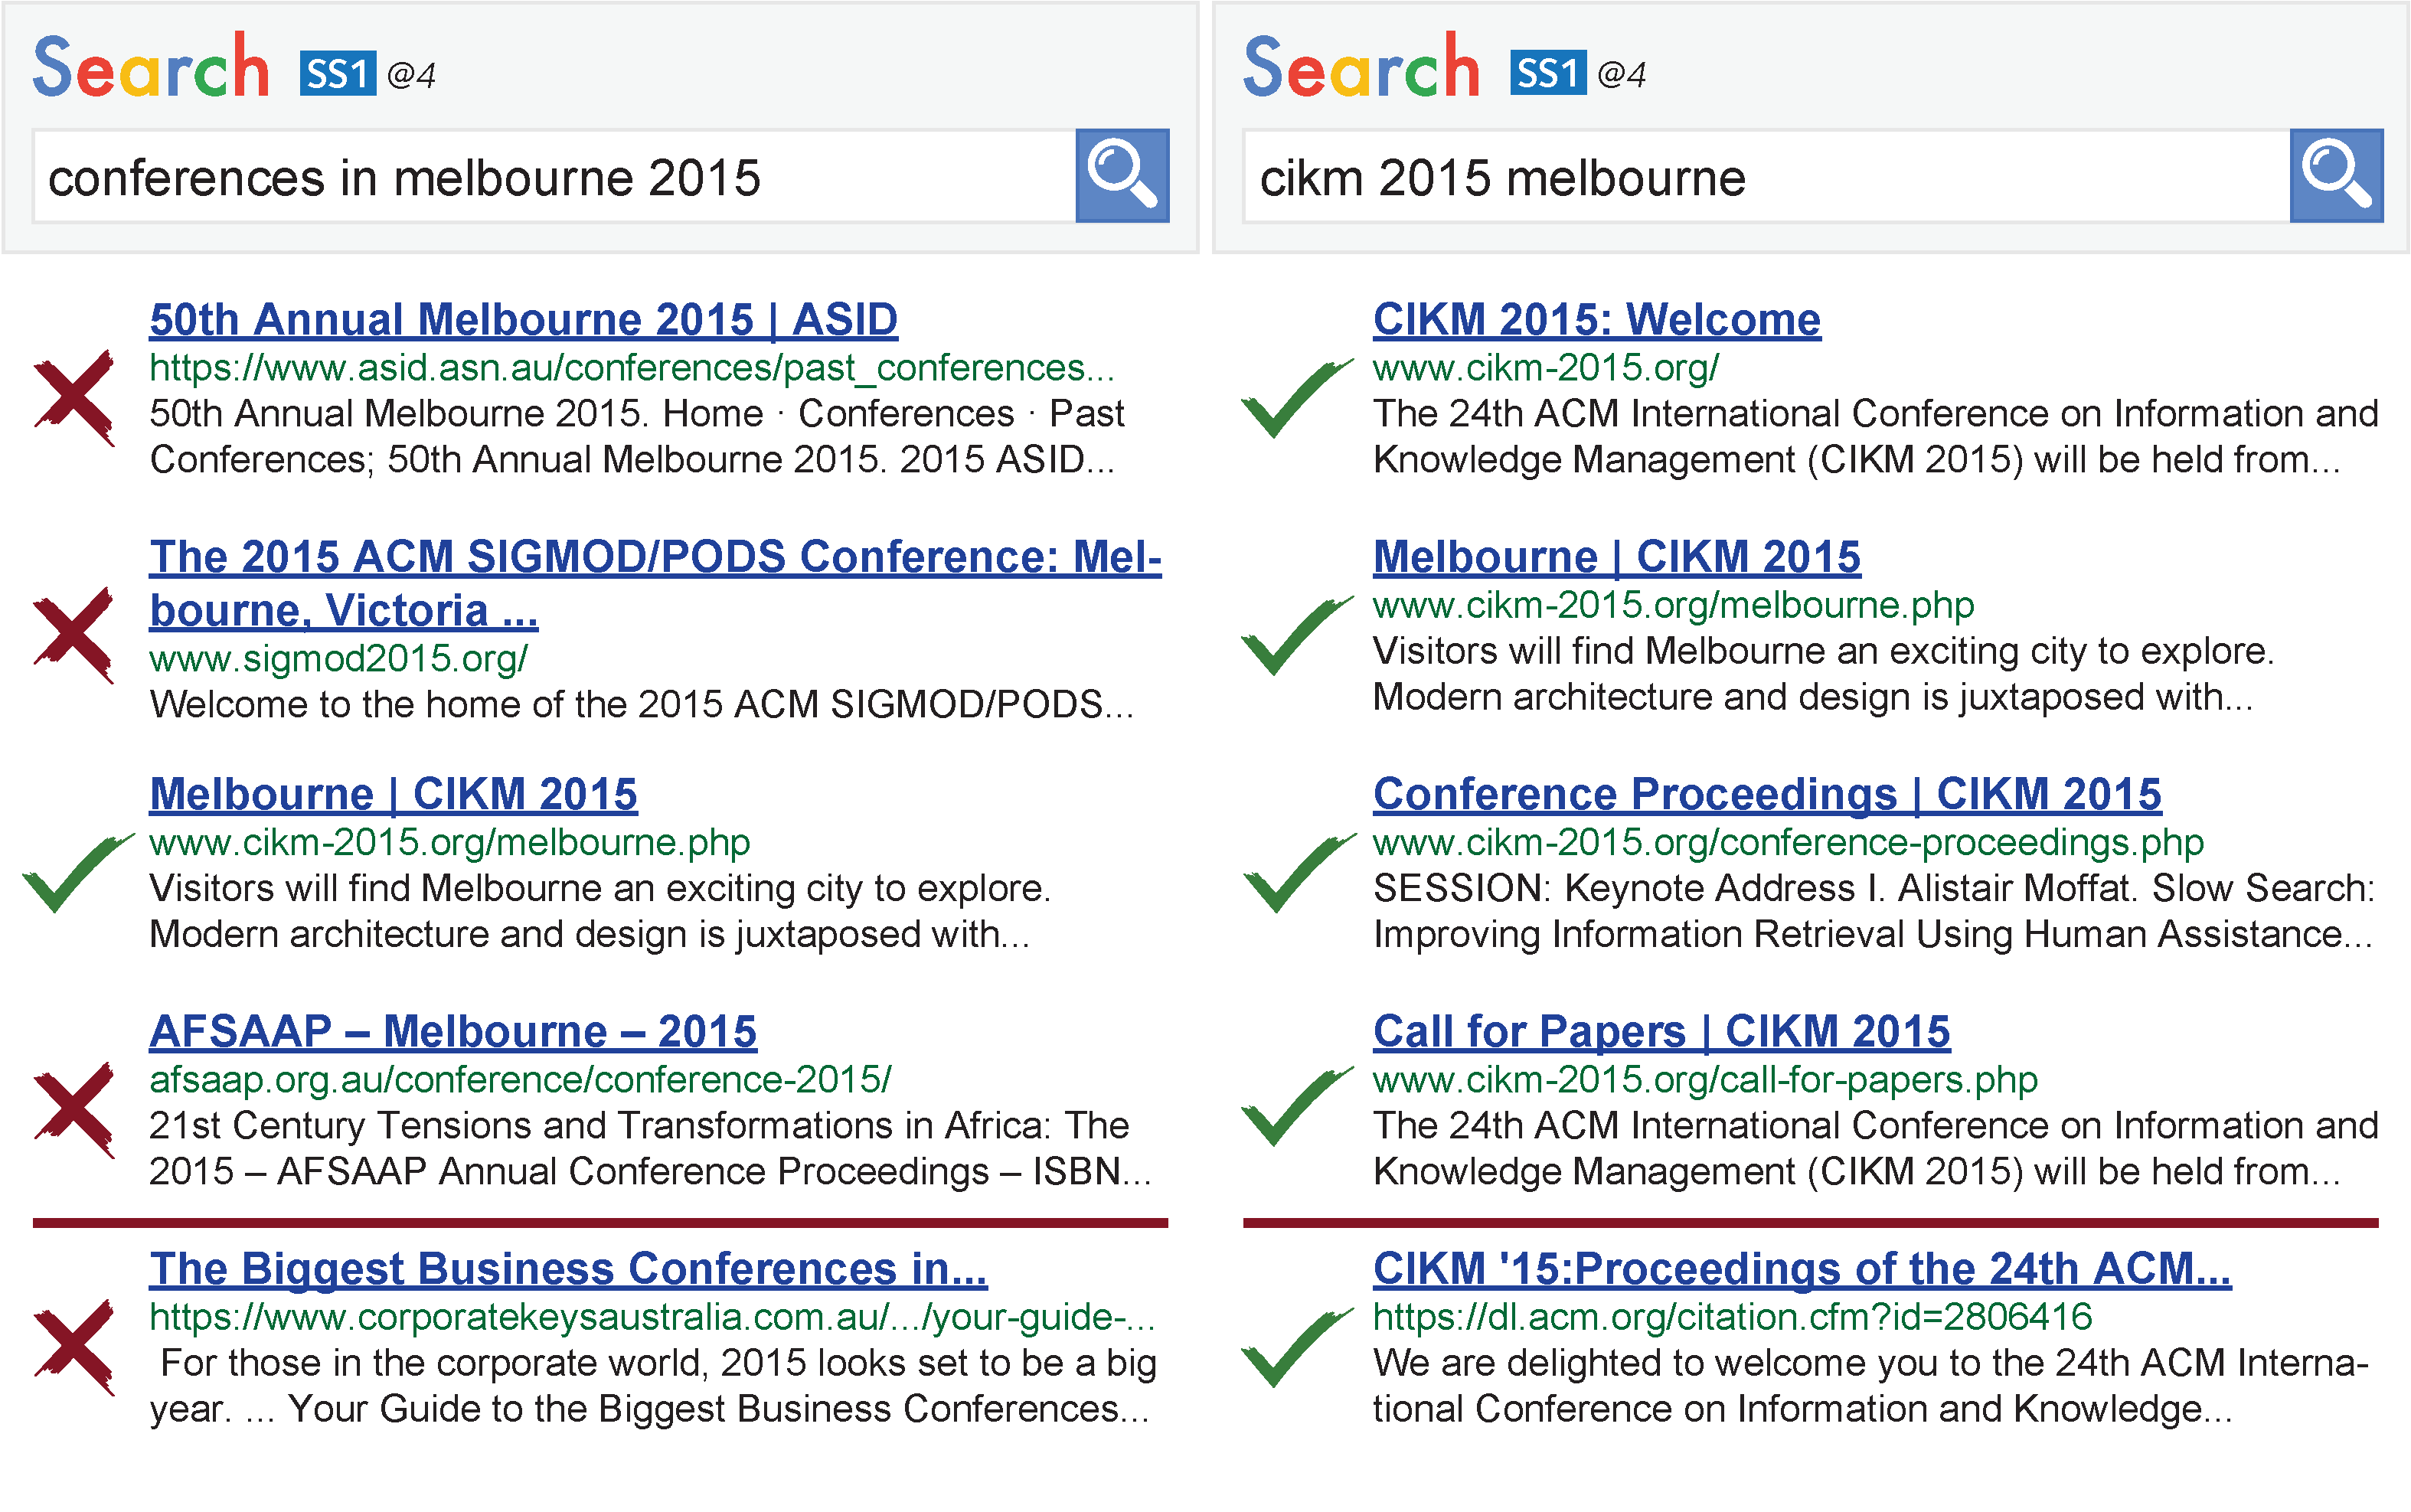
\includegraphics{figures/ch4-ss1.pdf}}
    \caption[Examples of the fixed depth stopping strategy, \blueboxbold{SS1}]{An example of the fixed depth stopping strategy, stylised in this thesis as \blueboxbold{SS1}. Here, a searcher has an information need for the conference \emph{CIKM 2015} in Melbourne, Australia. The left example shows the top five results for poor performing query, with few unattractive results (denoted by {
\includegraphics[height=\fontcharht\font`\d]{figures/ch0-cross.pdf}}); conversely, the right shows results for a query performing well, with many attractive results (denoted by {
\includegraphics[height=\fontcharht\font`\d]{figures/ch0-tick.pdf}}). With \stoppingstratbox{SS1}{4}, the searcher will stop at a depth of 4, regardless of the perceived relevancy of the content provided.}
    \label{fig:ss1}
\end{figure}

Given the description of the stopping strategy above, we note that the fixed depth approach is na\"{i}ve in the sense that documents up to rank $x_1$ are considered to be attractive to the searcher's given information need. On average, such a rule does make sense. When individual result lists are considered however, the approach would not be considered to be a sensible strategy to follow.

An additional drawback of such an approach is exposed when a searcher complying with such a strategy issues a poor performing query. This is demonstrated in Figure~\ref{fig:ss1}, with two~\glsplural{acr:serp} presented side by side. Given a searcher's desire to find pages that provide information regarding \emph{CIKM 2015}\footnote{CIKM 2015 was a conference held in Melbourne, Australia, in October 2015. The paper that initially proposed many of these stopping strategies~\cite{maxwell2015stopping_strategies} was indeed presented at this conference.}, two queries are issued: the query on the left yielding poorer results than the query on the right, as denoted by the ticks and crosses, for useful and unhelpful result summaries, respectively. With \stoppingstratbox{SS1-FIX}{4} set, four result summaries are always examined before stopping, regardless of their perceived usefulness. As a result of this, na\"{i}vely examining four documents for the query on the left is by and large a waste of the searcher's time.

\section{Searcher Frustration and Satisfaction}
With the baseline stopping strategy defined, we now consider more \emph{adaptive} stopping strategies. That is, stopping strategies that allow a searcher subscribing to them to adapt their stopping depth depending upon the result summaries that they observe. In this section, we propose three adaptive stopping strategies based upon a searcher's tolerance to non-relevance (frustration), and a simple goal-based strategy (satisfaction).

\subsection{Searcher Frustration}\label{sec:strategies:frustsat:frustration}
We first discuss our operationalisation of the frustration stopping heuristic, as outlined in Section~\ref{sec:stopping_background:heuristics:judgement:satisfaction_frustration}. Given a set of result summaries presented on a~\gls{acr:serp}, how many unattractive summaries would a searcher be prepared to examine before coming frustrated with the~\gls{acr:serp}, and abandoning it? This stopping heuristic attempts to address this question. Indeed, as detailed in Section~\ref{sec:stopping_background:heuristics}, a number of researchers have proposed stopping heuristics that consider unattractiveness.

The frustration heuristic intrinsically makes sense for exhaustive searches~\cite{kraft1979stopping_rules}. As an example, when tasked to find as many documents as possible related to different species of animals that are endangered, becoming disgusted with the presented~\gls{acr:serp} when a lack of animal species are shown would be a suitable point at which to break and reformulate a new query, or abandon the search session altogether.

From the heuristics defined by~\cite{cooper1973retrieval_effectiveness_ii} and~\cite{kraft1979stopping_rules}, we propose two variants of the frustration and disgust heuristics, \stoppingstratboxsingular{SS2-NT} and \stoppingstratboxsingular{SS3-NC}.

\begin{itemize}
    \item{\stoppingstratboxsingular{SS2-NT} Under this stopping strategy, the searcher will stop once they have observed $x_2$ unattractive result summaries.}
    
    \item{\stoppingstratboxsingular{SS3-NC} Similar to the stopping strategy defined above above, a searcher employing this stopping strategy will stop once they have observed $x_3$ unattractive result summaries \emph{in a row (contiguously)}.}
\end{itemize}

\begin{figure}[t!]
    \centering
    \resizebox{1\hsize}{!}{
    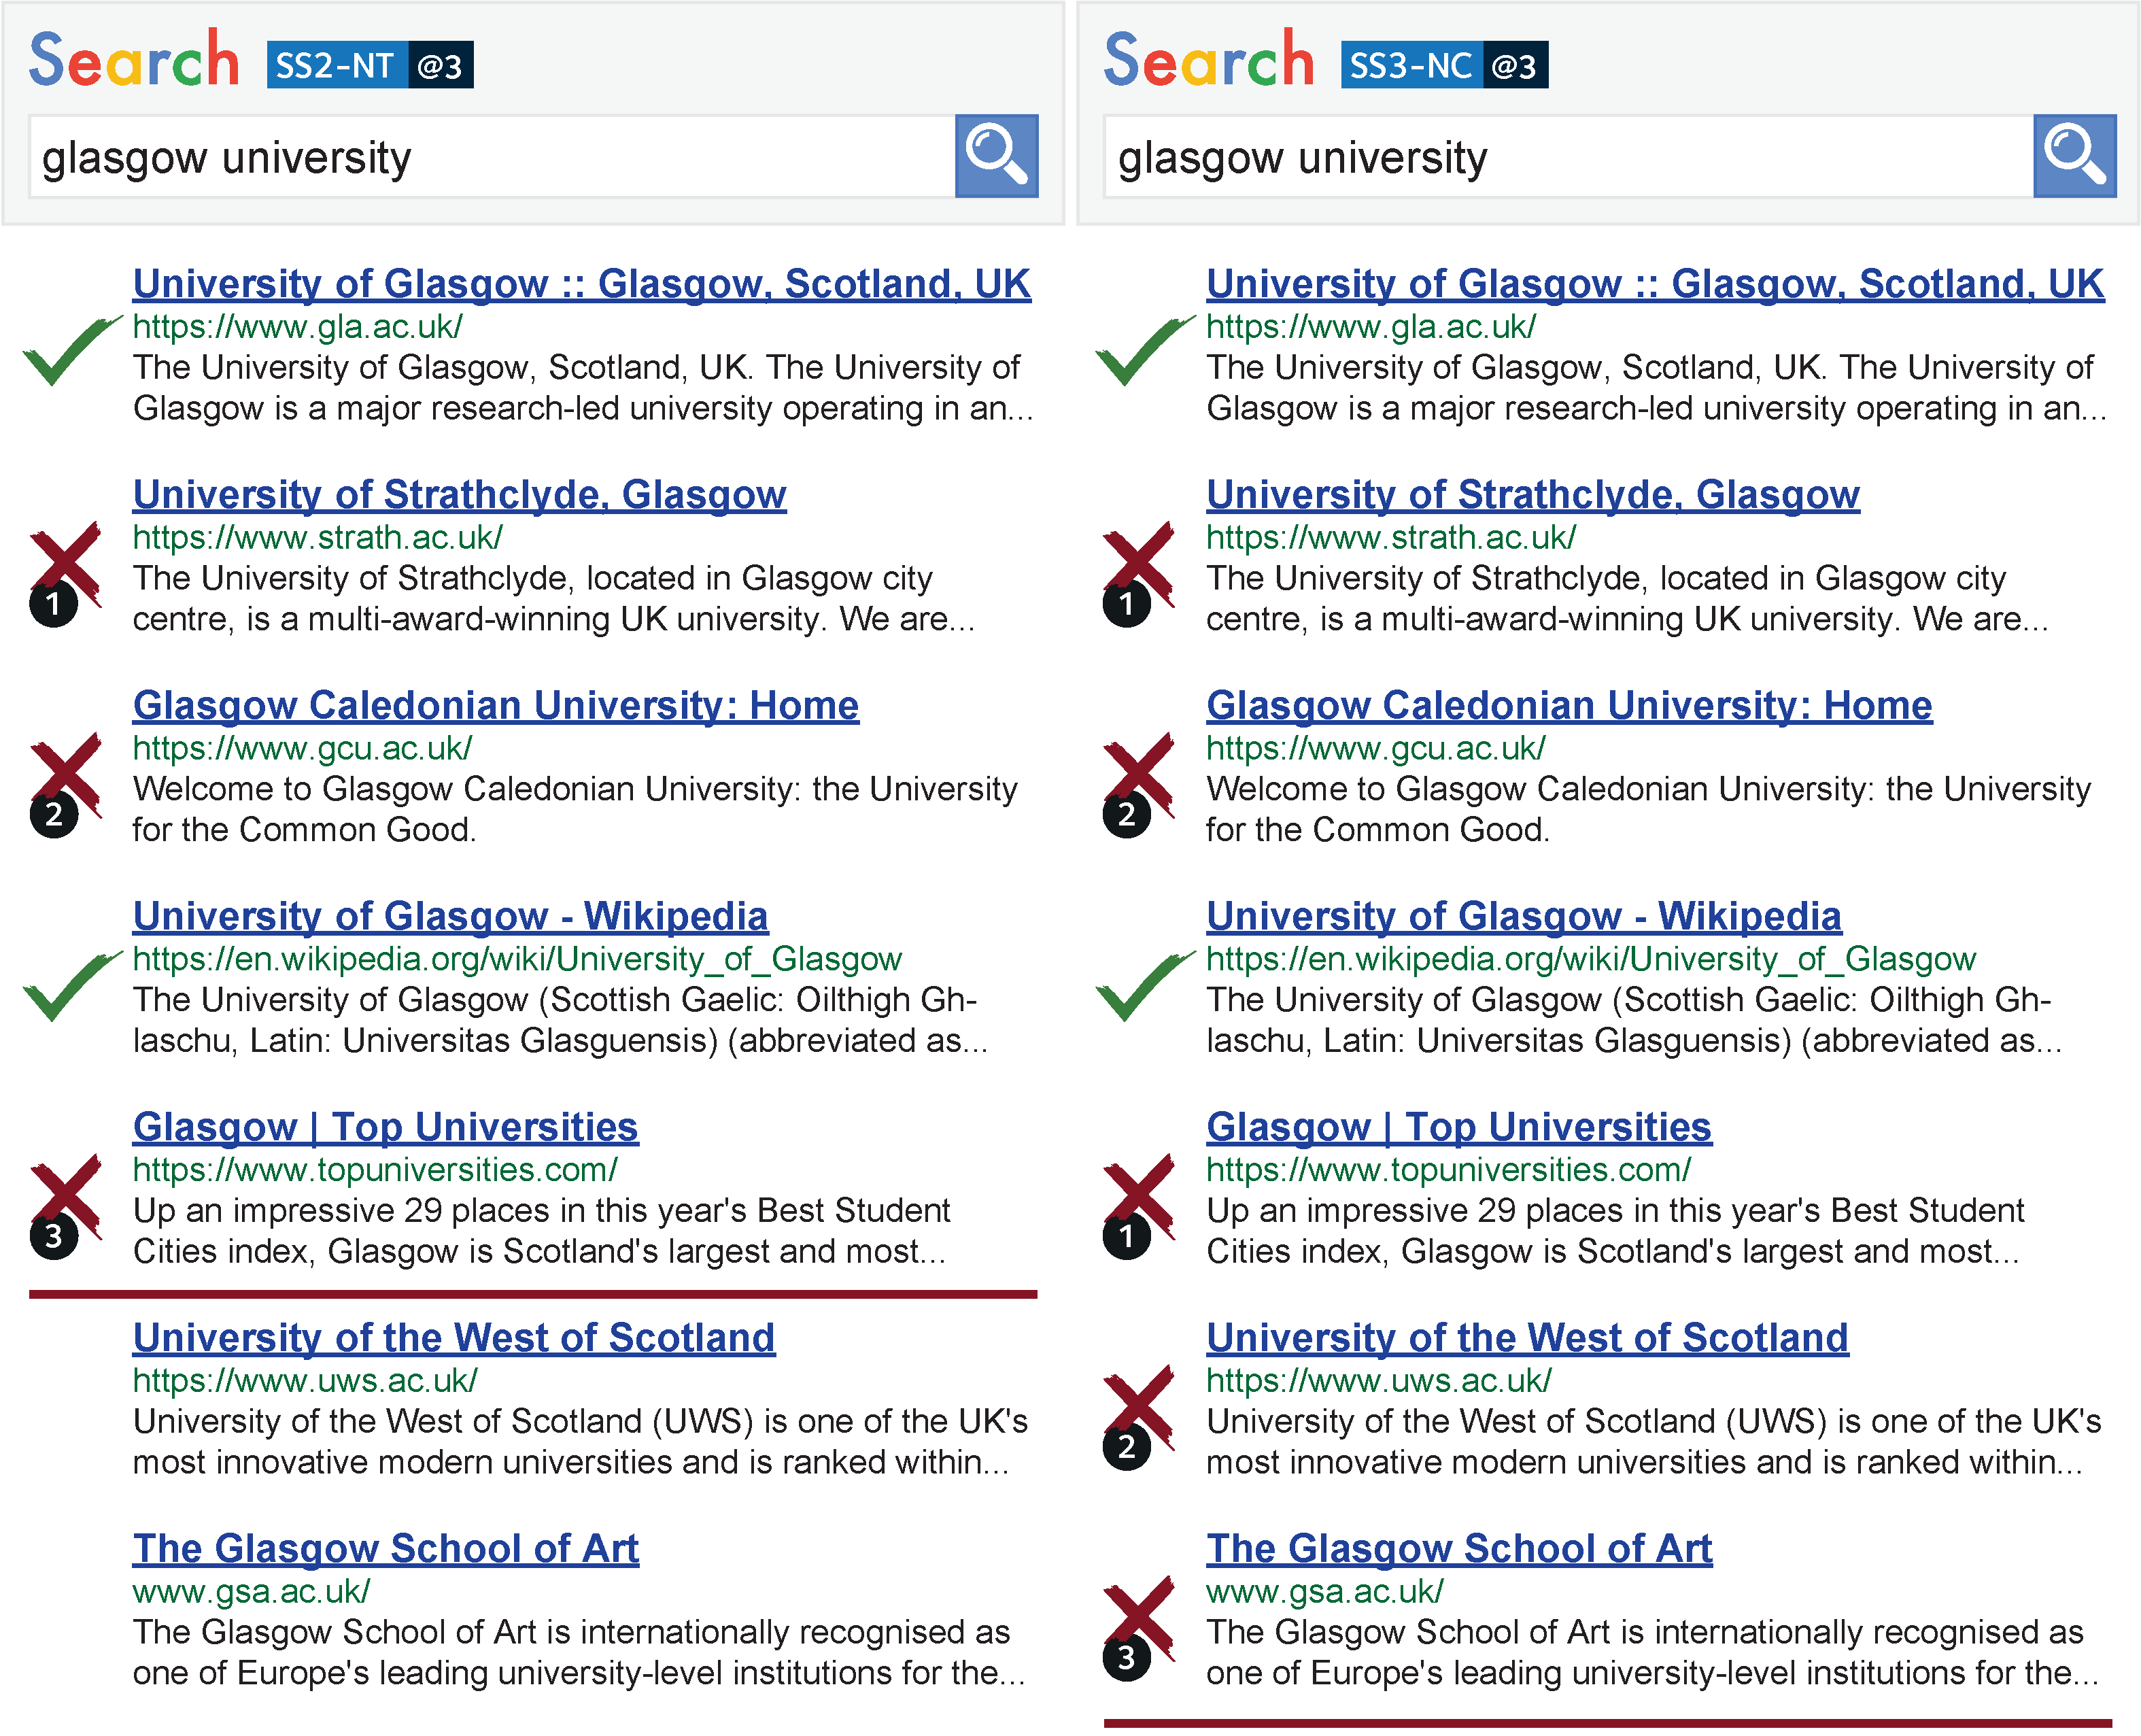
\includegraphics{figures/ch4-ss23.pdf}}
    \caption[Examples of frustration rules \blueboxbold{SS2-NT} and \blueboxbold{SS3-NC}]{An example of the two frustration rules, \blueboxbold{SS2-NT} (left) and \blueboxbold{SS3-NC} (right), both using a parameter of 3 unhelpful result summaries, under the same query and results. Given that \blueboxbold{SS2-NT} considers the total number of result summaries judged to be unhelpful, a searcher employing this stopping strategy would stop at rank 5 in the example above. Considering a set of contiguous unhelpful summaries, a searcher using \blueboxbold{SS3-NC} would stop at rank 7.}
    \label{fig:ss23}
\end{figure}

During the course of a search session, searchers may encounter the same documents, judged to be unattractive, in different ranked lists. For the stopping strategies, we include all previously observed summaries in the counts. As mentioned previously, these two stopping strategies are the first that we enumerate where a searcher would begin to \emph{adapt} their interactions with a ranked list of results, depending upon the performance of the underlying query that was issued. As such, this behaviour inherently makes these stopping strategies more realistic~\cite{moffat2013users_versus_models}. Figure~\ref{fig:ss23} illustrates this adaption in action, with the same query and associated results. On the left of the figure is an illustration of when a searcher employing \blueboxbold{SS2-NT} would stop, and on the right, an example of \blueboxbold{SS3}. We use \stoppingstratbox{SS2-NT}{3} and \stoppingstratbox{SS3-NC}{3}. Under \blueboxbold{SS2-NT}, a searcher would stop at rank 5, while a searcher would stop at rank 7 when employing \blueboxbold{SS3-NC}.

\cite{cooper1973retrieval_effectiveness_ii} highlights the above as one way of operationalising such a stopping strategy: by providing a pre-determined number of documents to stop at. The other approach, which we do not consider in this thesis, would be to allow a searcher to find a series of documents, then go back and count. Such an approach seems unnatural, with the former approach simulating a form of goal-based task. By varying the number of non-relevant documents to stop at, one will be able to attain a better understanding of how performance and searcher behaviours differ.

\subsection{Goal/Satisfaction Based}
Analogous to the frustration rule are the satiation-based stopping heuristics. Here, rather than focus on the frustration or disgust that a searcher might experience when confronted with unhelpful result summaries, satisfaction based rules -- explained in Section~\ref{sec:stopping_background:heuristics:judgement:satisfaction_frustration} -- consider a searcher encountering a number of \emph{useful} result summaries (or documents) before deciding to stop.

\begin{itemize}
    \item[\blueboxbold{SS4}] A searcher using this stopping strategy will stop examining content after encountering $x_4$ useful result summaries.
\end{itemize}

While demonstrated above in the context of snippet level stopping, such a strategy, depending upon the search task, may not be particularly useful when operationalised at this stopping decision point. For example, consider the scenario where a searcher issues a poor query, yielding next to no summaries deemed to be worthy of further examination. In this scenario, a searcher fully complying with \blueboxbold{SS4} may struggle to find enough documents to reach their goal, and this will waste time examining poor results. Such a stopping strategy may be better suited to an overall search goal (i.e. a session level stopping strategy), and deploying a more suitable stopping strategy for snippet level stopping decisions.


\subsection{Combining Frustration and Satisfaction}
Considering satisfaction and frustration based stopping heuristics,~\citealt{kraft1979stopping_rules} also proposed a \emph{combination heuristic} that combined both approaches together. Employing this heuristic, a searcher would stop when they became frustrated, or were satisfied by what they saw -- whatever comes first. As such, we can convert this into a stopping strategy, as described below.

\begin{itemize}
    \item[\blueboxbold{SS5}] A searcher utilising this stopping strategy will employ \blueboxbold{SS2} and \blueboxbold{SS4} to determine when to stop, ceasing their search on the~\gls{acr:serp} for the first stopping strategy whose criterion is met.
\end{itemize}

Note that we consider only a searcher's total tolerance to non-relevance (i.e. \blueboxbold{SS2}), not \blueboxbold{SS3}.


\section{Difference Threshold}
\todo{rewrite}
The next two stopping strategies are based upon the difference threshold heuristic. To operationalise this rule, we consider the difference between the text of the current snip- pet and the text of previously examined snippets. Here, the idea is that as simulated searchers examine snippets, they may encounter a snippet that is not sufficiently different from what they already have observed, meaning that they are unlikely to find new information. The searcher therefore stops and issues a new query. From this rule, we devised two separate stopping strategies where we computed the difference based upon term overlap and KL-Divergence scores.

\begin{itemize}
    \item[\blueboxbold{SS6}] This stopping strategy compares the occurrences of terms in a given snippet against all terms in previously examined snippets. The more terms that overlap, the greater the chance that the new snippet does not contain any new information. If $\frac{|s_{curr} \cup s_{prev}|}{|s_{curr}|} > x_6$, the new snippet is considered too similar to previously examined content. The searcher will then move to the next query. Here, $s_{curr}$ denotes the terms of the current snippet, $s_{prev}$ denotes terms from all previously observed snippets, and $x_6$ is the threshold at which the searcher will stop.
\end{itemize}

\begin{itemize}
    \item[\blueboxbold{SS7}] This stopping strategy considers KL-Divergence as a means for comparing a given snippet against previously observed snippets. If the resulting value is less than threshold $x_7$, then the snippet is considered too similar to previously seen content, and the searcher stops, moving to the next query.
\end{itemize}

When implementing \textbf{\emph{SS4}} and \textbf{\emph{SS5}}, we considered the \emph{per-query difference} and the \emph{per-session difference}. For the per-query variant, previously observed text consisted of the first snippet, thus meaning that the simulated searcher always considers at least two snippets before stopping. For the per-session variant, all previously seen snippets over the simulated search session are used. In this paper, we will only report the per-query variants of \textbf{\emph{SS4}} and \textbf{\emph{SS5}}, as both performed somewhat better than their per-session variants in a pilot study. A number of other variants were also considered but not explored, such as using the document and snippet text, and using only text from snippets considered relevant. To compute the KL-Divergence, we used a \emph{Maximum Likelihood Estimate (MLE)} of the term distribution given the new snippet, and all the previously examined snippets. We also explored smoothing the distribution with the probabilities of each collection used. However, this approach was not used; performance was not increased, only complexity.

\section{\gls{acr:ift} and Optimal Foraging}
We look at IFT now -- so we have the optimal stopping rule, as previously discussed in Section~\ref{} and a number of rules borrowed from ecology that consider the time a searcher will spend examining a \emph{patch} before moving on.

\begin{itemize}
    \item[\blueboxbold{SS8}] With this stopping strategy, a searcher is assumed to have some idea of the average rate of gain (denoted as $x_6$). If the rate of gain from the observed documents thus far does not exceed $x_6$, the searcher then stops and proceeds to issue the next query.
\end{itemize}

To determine the rate of gain at the current snippet, we first computed the \emph{Discounted Cumulative Gain (DCG)} $g$ received from the observed documents up to that point in the ranked list at position $i$. We then divided $g$ by the total time taken, i.e. $i*t_d +t_q$, where $i$ represents the rank, $t_d$ is the time taken to examine a document, and $t_q$ is the time taken to issue a query. This estimate is very dependent upon the first document. For example, if the first document is non-relevant, then the gain is zero, and thus the simulated searcher would immediately stop when $x_6>0$. We also included another parameter which specifies how many snippets they should first consider before making their decision based on the rate of gain\footnote{\scriptsize{This parameter was set to 2 for this study - refer to Section~\ref{sec:method:stopping}.}}. This would essentially mean that the simulated searcher would look at $y_6$ snippets/documents, and then decide to continue with the current query.

\section{Time-Based Strategies}
More directly connected to stopping is the Information Patch Model~\cite{pirolli1999ift} which is derived from Optimal Foraging Theory. The stopping rule from Foraging Theory is based on Charnov's Maximal Marginal Theorem~\cite{charnov1976mvt}, which states that when the rate of gain within the patch falls below the average rate of gain in the environment then the forager will stop (see Figure~\ref{fig:ift_patch}). This lead to the \emph{instantaneous intake} rule, where a forager will leave when their rate of gain falls below a given threshold (refer to Figure~\ref{fig:ift_patch}). However, it is often difficult to operationalize this rule/theorem in practice. Instead several other stopping rules that influence patch leaving decisions have been developed in Foraging Theory ~\citet{stephens1986foraging_theory}, which approximate the theorem. These  include: the \emph{number rule}~\cite{gibbs1958number_rule}, where a forager stops after finding $n$ prey (similar to the satisfaction~\cite{cooper1973retrieval_effectiveness} and satiation rules~\cite{kraft1979stopping_rules}); the \emph{time rule}~\cite{krebs1973time_rule}~\cite{charles1972behaviour}, where a forager stops after $x$ seconds; the \emph{leave after an $x$} rule~\cite{krebs1974leave_after_rule}, where a forager would stop after $x$ seconds of unsuccessfully finding anything. A study of different \emph{patch types} (i.e. where the density of prey varies), was conducted by~\citet{mcnair1982gut_mvt} who found that across different patch types, different stopping rules worked better in different environments~\cite{mcnair1982gut_mvt, green1984oft_stopping, iwasa1981prey_distribution}. Consequently, a combination rule was devised where in a patch that is fruitful early on, a satisfaction/satisficing rule would perform well; otherwise employing the leave after $x$ rule would work best. In this paper, we develop several new stopping strategies based on these rules from Optimal Foraging Theory and also introduce a SERP level stopping decision component that considers the information scent of the page before examining the snippets in detail.

\begin{figure}[t!]
    \centering
    \resizebox{1\hsize}{!}{
    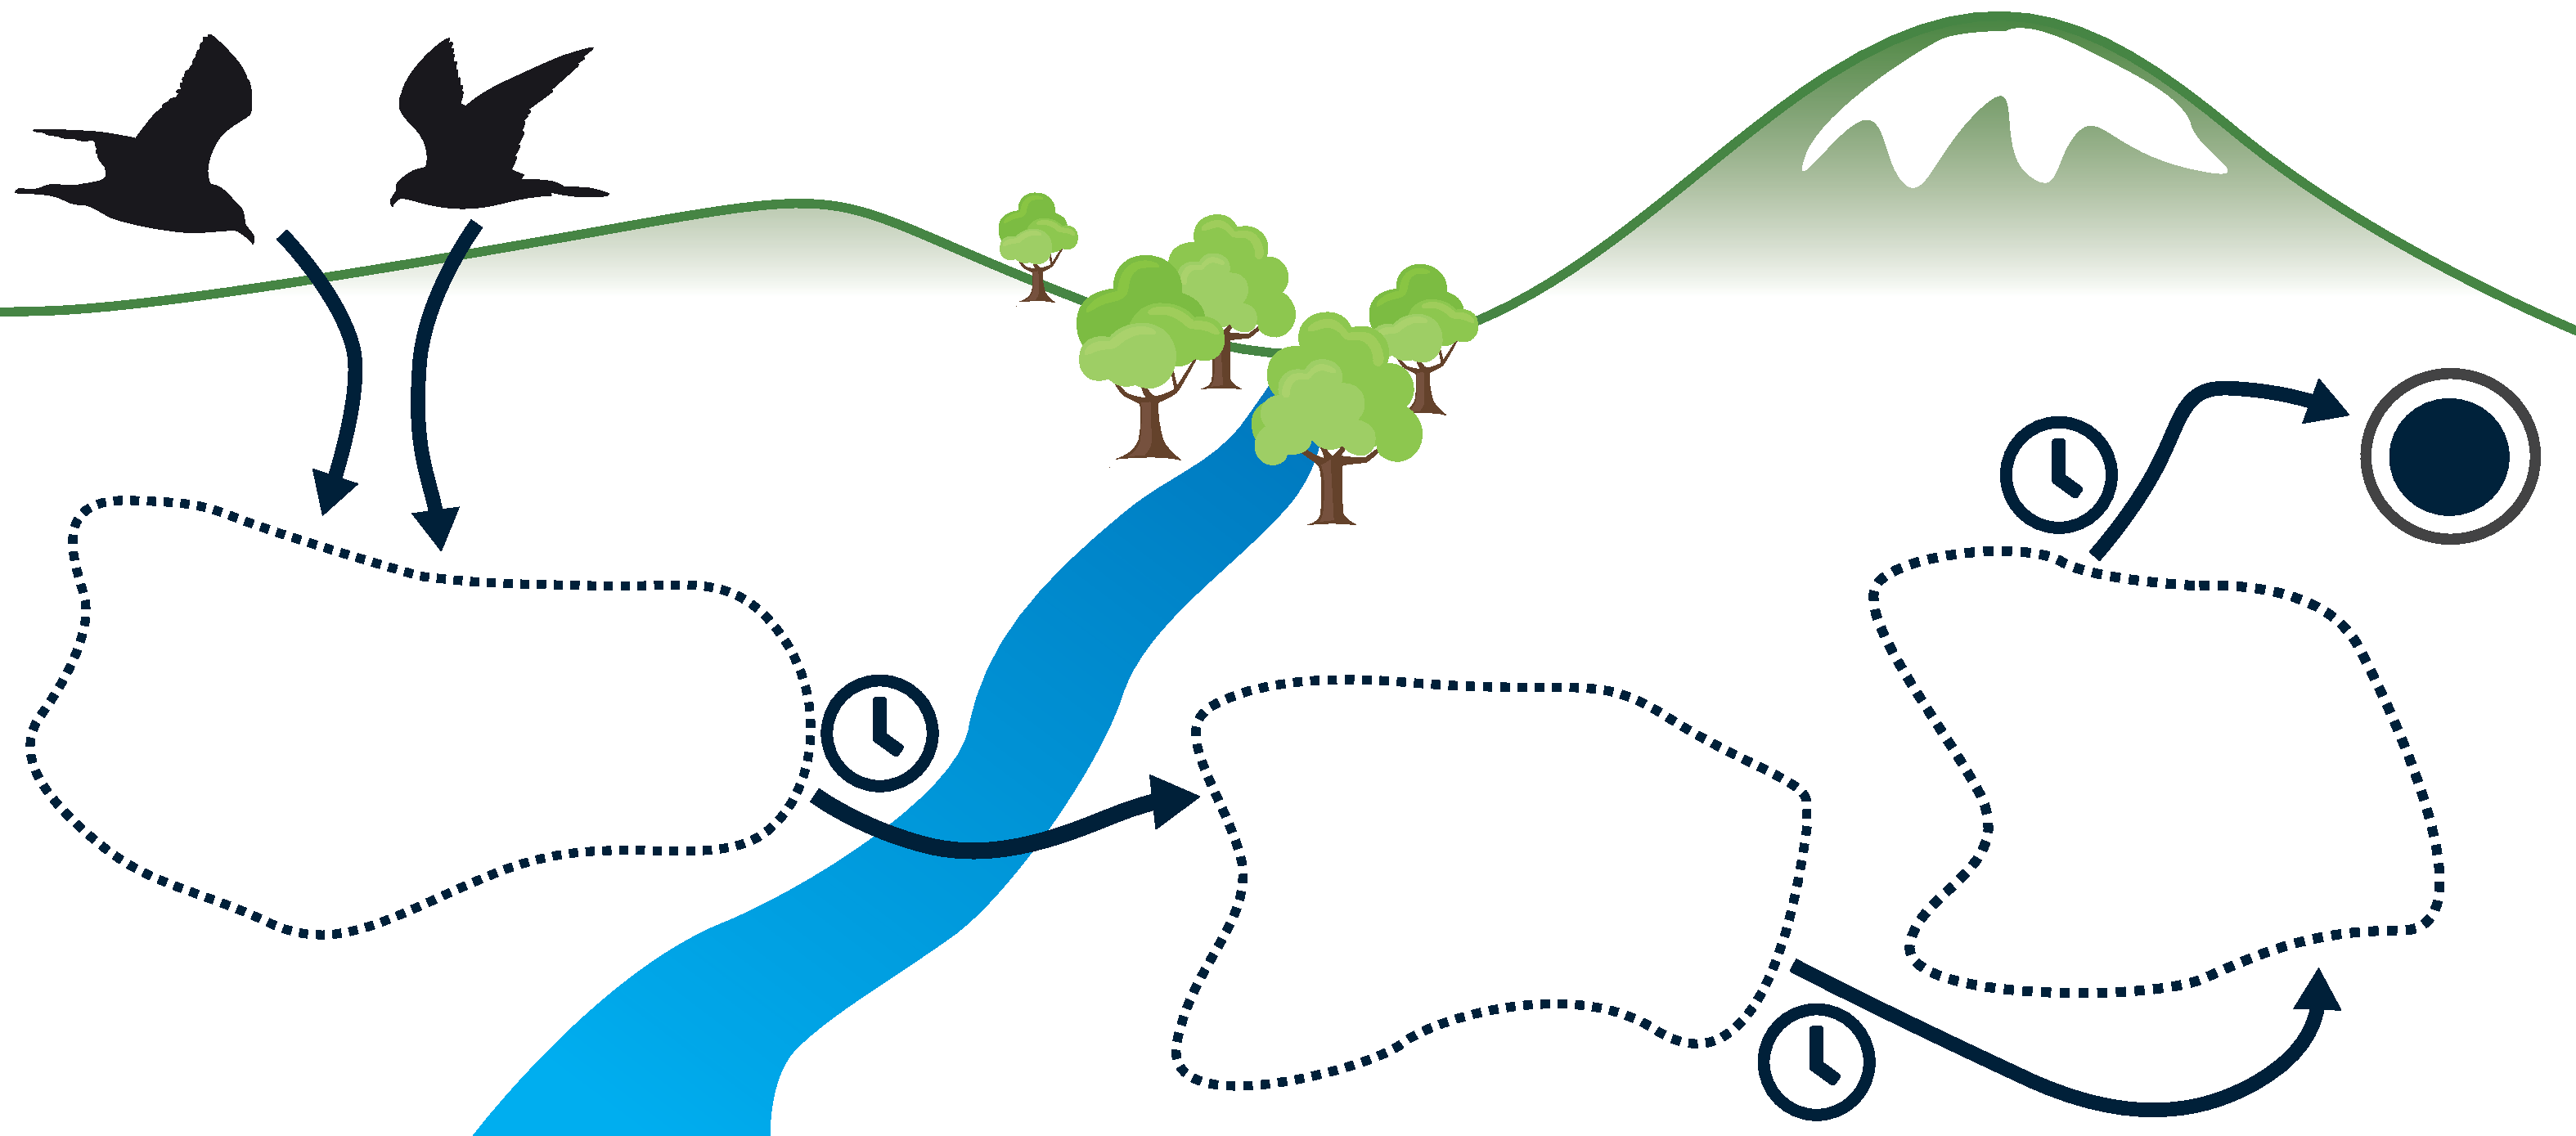
\includegraphics{figures/ch4-gut.pdf}}
    \caption[Give Up Time]{The give up time}
    \label{fig:gut}
\end{figure}

The next two strategies are based on the \emph{time} rule and the \emph{Giving Up} rule~\cite{gibbs1958number_rule}:

\begin{itemize}
    \item[\blueboxbold{SS9}] Employing this stopping strategy, a searcher will leave a SERP after $x_9$ seconds have elapsed from first entering it.
\end{itemize}

\begin{itemize}
    \item[\blueboxbold{SS10}] A searcher employing this strategy will stop after $x_10$ seconds have elapsed since a snippet judged to be relevant was found. If no relevant items have been encountered on the given SERP, then the searcher will stop after $x_9$ seconds have elapsed since arriving at the SERP.
\end{itemize}

These stopping strategies are similar to the frustration based strategies previously proposed (i.e. \textbf{SS2} and \textbf{SS3}) except bound by time~\cite{gibbs1958number_rule}. As mentioned earlier ~\citet{mcnair1982gut_mvt} studied how animals would change their stopping strategies based on their initial evaluation  of the patch, where his suggested combination rule would be as follows.

\begin{itemize}
    \item[\blueboxbold{SS11}] When encountering a SERP expected to yield a high volume of relevant content early on (high scent), the searcher will employ the satisfaction stopping strategy \textbf{SS8S}. If the SERP however yields relevant items over greater depths, or is judged to be of poor quality (low scent), the giving-up stopping strategy, \textbf{SS10G}, is used instead.
\end{itemize}

The combination rule tries to ensure that searcher avoids wasting time on patches with a low yield, but capitalize on patches with a high yield. In the following section, we shall describe the simulated analysis to compare the existing and proposed stopping strategies.

\section{\gls{acr:ir} Evaluation Measures}
As previously mentioned most evaluation measures implicitly encode some stopping model (e.g. P$@$10 encodes SS1$@$10). Two measures that have been recently proposed that explicitly encode a stopping model are \textbf{RBP}~\cite{moffat2008rbp} and \textbf{INST}~\cite{bailey2015inst, moffat2015inst}. 
Under \textbf{RBP}, the decision to continue to the next results is based on the patience parameter (e.g. the probability of continuing), while under \textbf{INST} the probability of continuing is based on how many the documents the searcher expects to encounter, how many they have encountered and their current rank - essentially the probability of continuing decreases as they encounter more relevant information, and as they progress further down the ranking.

\begin{itemize}
    \item[\blueboxbold{SS12}] RBP
\end{itemize}

\begin{itemize}
    \item[\blueboxbold{SS13}] INST
\end{itemize}

The satisfaction stopping strategy \textbf{SS8S} was set to consider $1$ to $7$ (hence providing values for $x_8$). A maximum of seven was chosen as this was closest integer to the mean number of documents marked by subjects in the log data. With our \textbf{INST} stopping strategy employing a similar approach, considering the ``number of useful pages that the searcher expects they will need''~\cite{moffat2015inst}, we subsequently set $T$ in INST to the same range. For our other baseline, \textbf{RBP} considers a \emph{patience factor} that influences the depth to which a searcher is prepared to tolerate examining to. Using the log data we estimated the patience of users to be approximately $p=0.9087$. In this study, examined patience from $0.8$ to $0.95$ in steps of $0.05$, and also $0.99$.
    % %!TEX TS-program = xelatex
%!TEX root = ../../maxwell2018thesis.tex

\chapter[General Methodology]{General Methodology}\label{chap:method}
In Part~\ref{part:context}, we will be exploring how an individual's stopping behaviours vary under different search contexts. In this chapter, we provide an overview of the general methodology that we deploy in subsequent chapters. As per the overview provided in Chapter~\ref{chap:intro}, our methodology is divided into four main areas:

\begin{itemize}
    \item{conducting a \blueboxbold{user study} to examine real-world searcher behaviours;}
    \item{extracting the key \blueboxbold{interaction data and performance measures} from the user study;}
    \item{using the aforementioned data to ground a series of \blueboxbold{simulations} that attempt to replicate the user studies; and}
    \item{\blueboxbold{evaluating} the performance of the simulated users, as well as \blueboxbold{comparing} the simulated user behaviours against those of their real-world counterparts.}
\end{itemize}

We now discuss each of these different tasks in greater depth, highlighting the key decisions that we have made, and discuss supporting literature for our choices.

\section{Test Collection, Topics and Search Engine}\label{sec:csm:methodology:collection}
Central to any~\gls{acr:ir} experiment is a corpus of documents (refer to Section~\ref{sec:ir_background:basics:indexing}) with which subjects participating in the experiment can issue queries against. In conjunction with the document corpus, a number of topics are also used to provide simulated information needs.

For the contributory chapters of this thesis, all work detailed uses the TREC AQUAINT corpus, consisting of over one million news articles (referred to as documents) from the period ranging 1996 to 2000. All of the news articles were collected from three newswires, namely: the \emph{Associated Press (AP);} the \emph{New York Times (NYT);} and \emph{Xinhua}. More contemporary collections could have been used; the reasons for selecting an older were twofold: \emph{(i)} using such a collection enabled us to easily evaluate the performance of subjects; and \emph{(ii)} employing the AQUAINT corpus provides continuity with a prior line of research using this collection, as shown by~\cite{azzopardi2013query_cost}, for example.

Five topics were also selected from the 50 provided in the \emph{TREC 2005 Robust Track,} as outlined by~\cite{voorhees2006trec_robust}. These topics were selected based upon evidence from a previous user study (of similar nature) conducted by~\cite{kelly2015serp_size}. Evidence showed that the topics offered similar levels of difficulty. The five topics, along with a short description of what constitutes a relevant document, are listed below. These summaries are derived from the TREC topic descriptions that are provided as part of the TREC 2005 Robust Track -- Figure~\ref{fig:topics} illustrates three examples of topic descriptions.

\begin{figure}[t!]
    \centering
    \resizebox{1\hsize}{!}{
    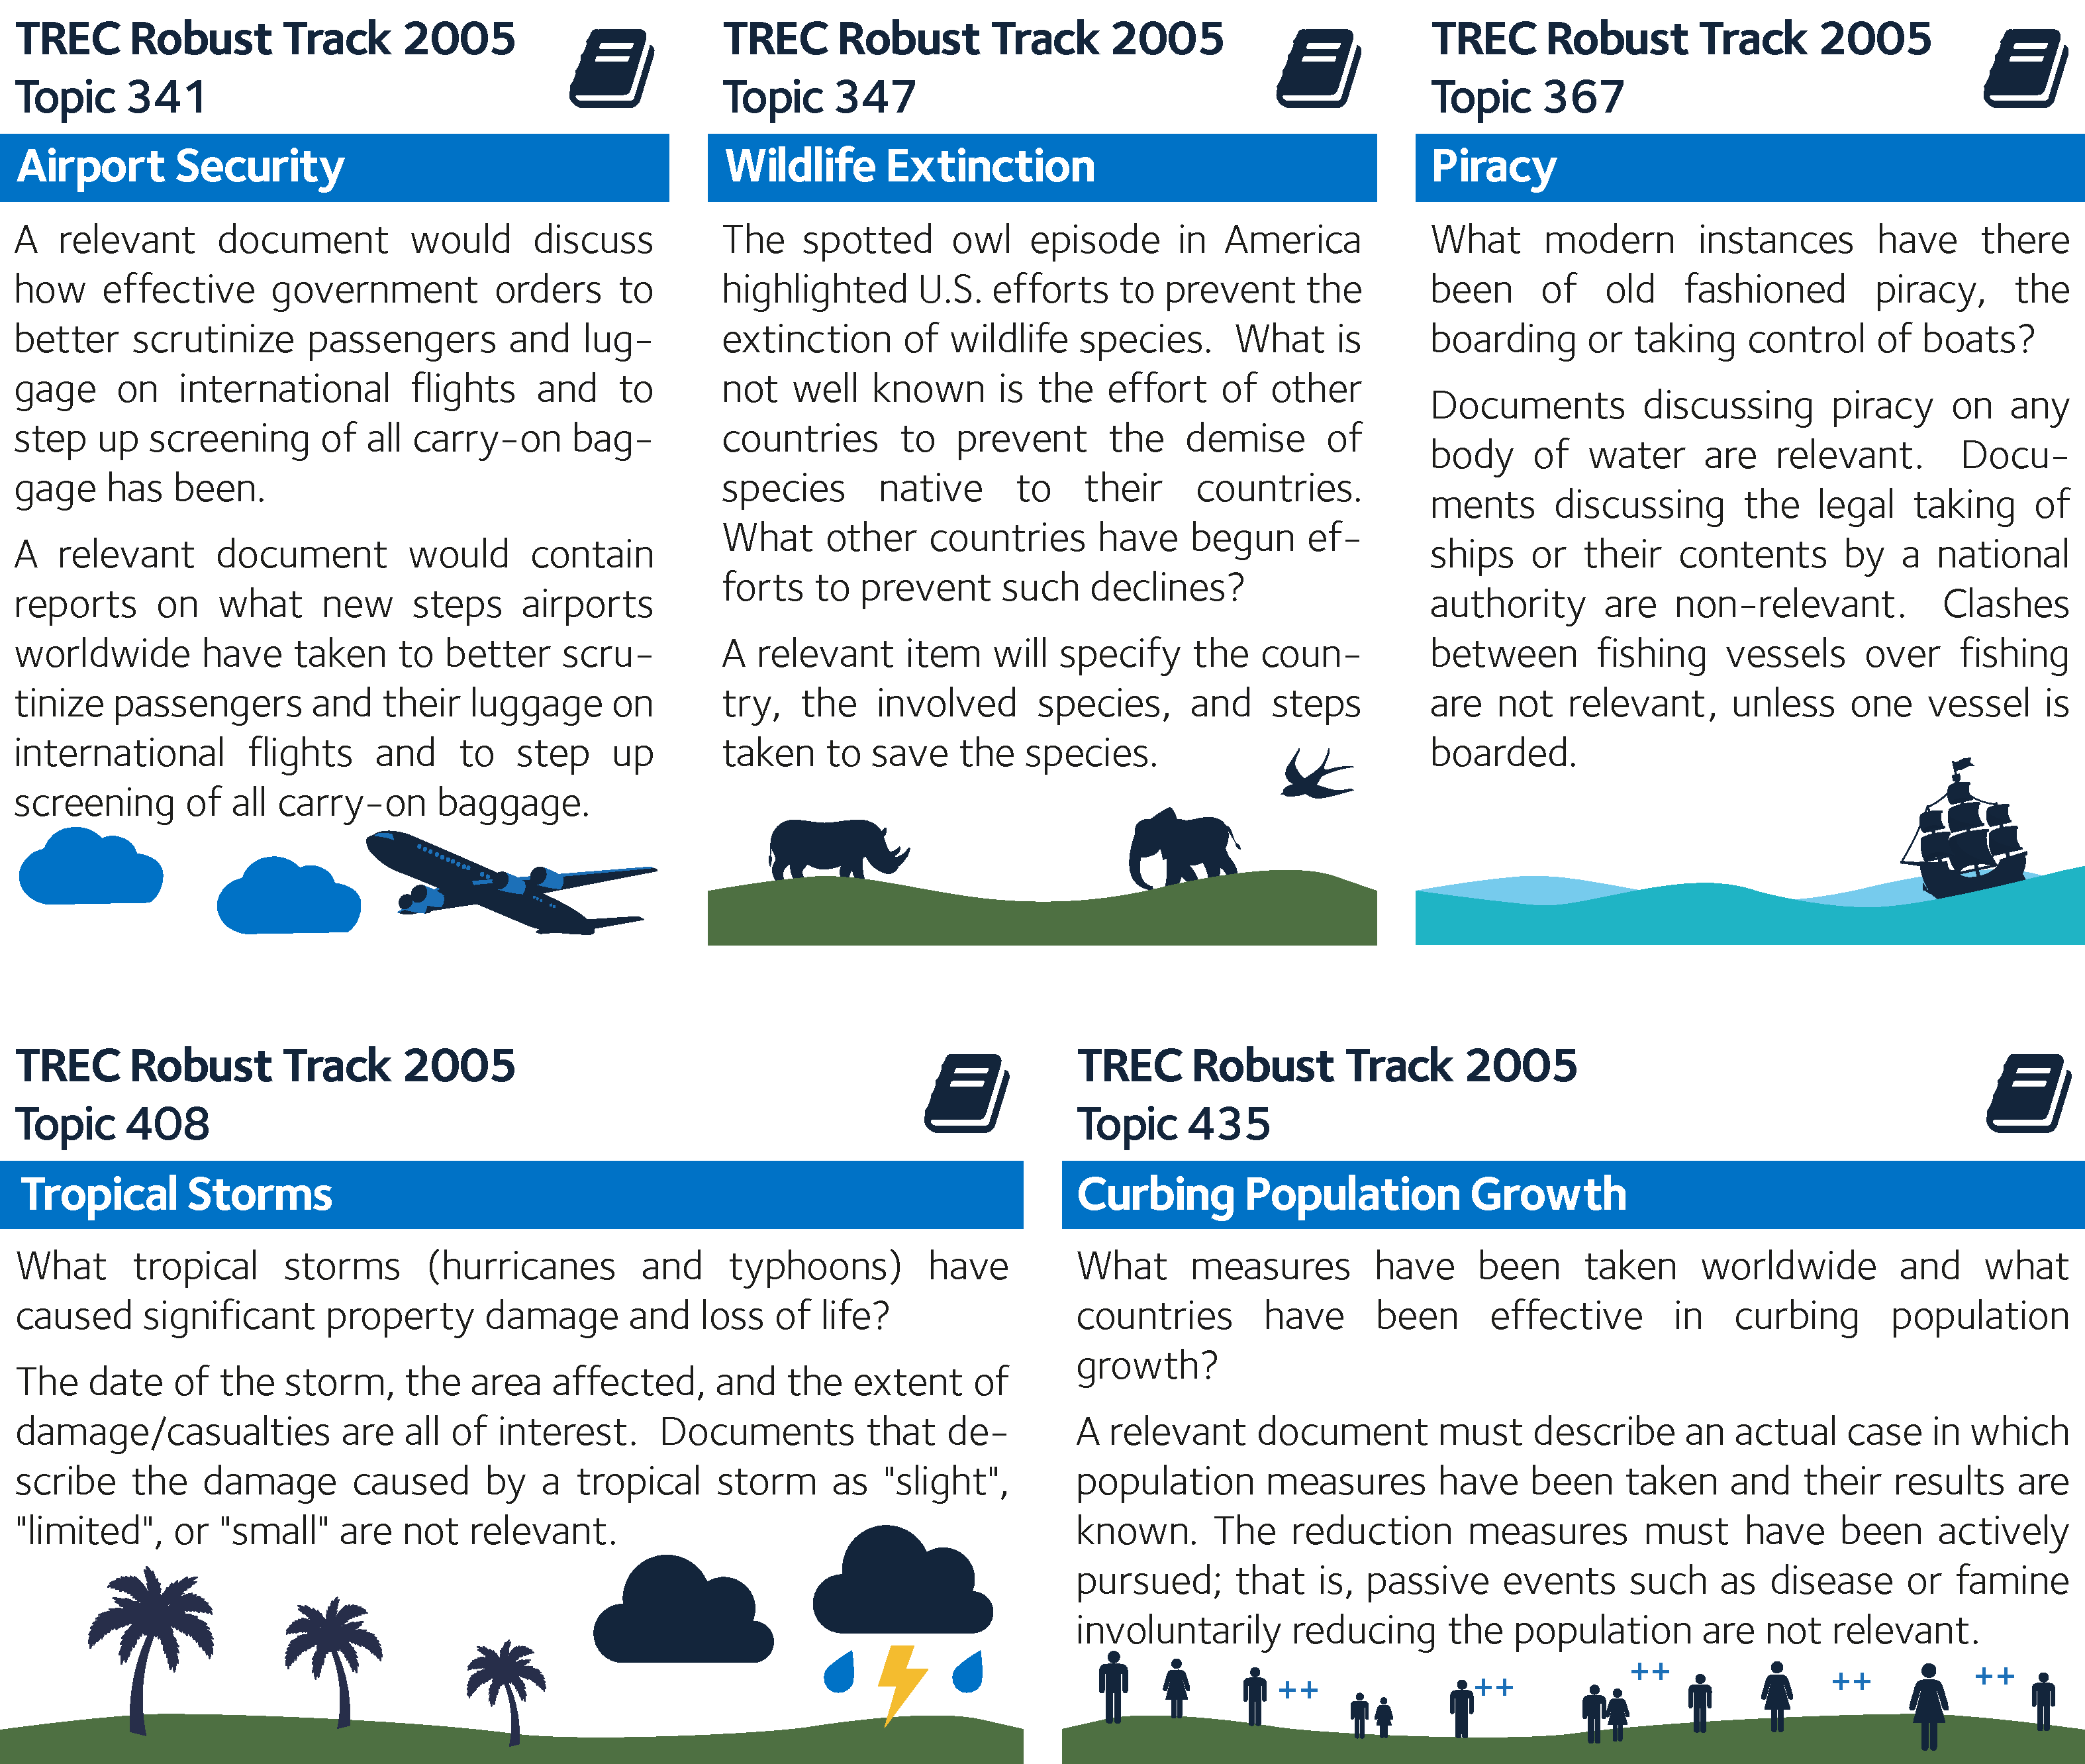
\includegraphics{figures/ch4-topics.pdf}}
    \caption[Examples of TREC Topics]{Three examples of \emph{TREC topic descriptions}, as outlined in Section~\ref{sec:csm:csm:flow}. Topics are extracted from the \emph{TREC 2005 Robust Track,} as outlined by~\cite{voorhees2006trec_robust}. Descriptions provide an explanation as to what constitutes a relevant (and often non-relevant) document.}
    \label{fig:topics}
\end{figure}

\begin{itemize}
    
    \item[]{\blueboxbold{Topic 341 – Airport Security} This topic considers relevant documents as those that discuss additional security measures that were taken by international airports around the world. Relevance is only denoted when a document discusses measures that go beyond the basic passenger and carry-on luggage screening. For example, AQUAINT document \texttt{NYT19980616.0123} discusses \emph{San Francisco International Airport's} attempts at introducing a \emph{robot sniffer,} attempting to look for nitroglycerine in luggage.}
    
    \item[]{\blueboxbold{Topic 347 – Wildlife Extinction} As the title of the topic suggests, this topic concerns wildlife extinction, and what efforts have been taken by countries other than the United States to counter the decline in endangered wildlife. Relevant documents explicitly mention the country, the species of animal, and the efforts the state or other governmental agency took to prevent decline in numbers. For example, document \texttt{XIE20000531.0205} discusses the breeding programme undertaken by China to bolster the number of Siberian Tigers in its jurisdiction.}
    
    \item[]{\blueboxbold{Topic 367 – Piracy} Instances of modern piracy are considered relevant to this topic -- not in the sense of software piracy, but the act of a water going vessel being boarded by individuals wishing to hijack it. Document \texttt{APW19980601.1065} provides an example of this -- the \emph{Petro Ranger}, a large fuel tanker, was boarded by pirates in 1998 in the South China Sea. To be relevant to the topic, the name of the vessel and the body of water it was hijacked on must be mentioned -- those discussing instances of when states intercepted vessels are not relevant.}
    
    \item[]{\blueboxbold{Topic 408 – Tropical Storms} Documents discussing major tropical storms are to be considered relevant, where the storm is reported to have caused significant damage and a large number of casualties. This is a particularly timely topic for the document corpus considered, as the 1998 hurricane season in the Caribbean has been reported to be one of the most costly -- both in terms of damage caused and lives lost -- in history.\footnote{This is reported by the US \emph{National Oceanic and Atmospheric Administration (NOAA),} as seen at \url{http://www.outlook.noaa.gov/98hurricanes/}. \urlaccessed{2018-05-18}} Document \texttt{APW19980921.1265} for example discusses the effects on Puerto Rico of Hurricane Georges in September 1998, leaving -- at the time of reporting -- three dead, many houses damaged, and thousands homeless.}
    
    \item[]{\blueboxbold{Topic 435 – Curbing Population Growth} The final topic considers efforts that have been made by countries around the world to control the ever increasing human population. Documents discussing this issue are only relevant to the topic if the results to a case have been made public, and a reduction in population has been actively pursued. The document must mention the country, the As such, events like famines are not relevant. A perhaps well known example of such a phenomenon is the one child policy that was pursued by China in the late 20\textsuperscript{th} century. Document \texttt{NYT19981031.0070} discusses the Chinese government's efforts to curb its expanding population at the time, with sexual education and heavy financial penalties for additional children. These efforts were shown to lead to a reduction in population, although whether this actually occurred is open to debate.}
    
\end{itemize}

For all user studies reported in this thesis, we selected topic \blueboxbold{367} as a \emph{practice topic,} permitting the participating subjects to familiarise themselves with the experimental system used. As such, we do not report any results from interactions that took place with this topic -- comparisons between simulated and actual searcher behaviours are also omitted. 

All queries submitted during experiments were also handled with the \emph{Whoosh~\gls{acr:ir} Toolkit}.\footnote{\emph{Whoosh} can be freely acquired using the \texttt{pip} \emph{Python} package manager -- documentation for Whoosh is available online at \url{http://whoosh.readthedocs.io/en/latest/intro.html}. \urlaccessed{2018-05-18} The corpus was indexed with Whoosh \texttt{2.7.4}.} Using the toolkit, we indexed the AQUAINT document collection, applying Porter stemming. Stopwords -- from Fox's classical stopword list -- were also removed (refer to Section~\ref{sec:ir_background:basics:indexing} for more information on the indexing process). For this index, we also removed documents with \todo{duplicate titles}. This is an issue, especially with documents originating from a newswire. A document discussing an ongoing event may be continually revised as new information arises, leading to multiple revisions. \todo{For documents with duplicate titles, we retained the document with the latest timestamp.}

With an index weighing in at 800MB, consisting of $128,894$ documents. \todo{What else did we do to reduce this number?} We could then issue queries against the index. All ranked results from queries were computed with the BM25 algorithm, where $\beta=0.75$. Terms in the queries issues were implicitly \texttt{AND}ed together to restrict the set of retrieved documents to those that only contained all of the query terms. This was chosen to reduce the size of the returned set -- most search systems employ such an implicit approach.

\section{User Study Methodology}\label{sec:method:user_study}
Using the document collection, topics and search engine outlined above, we now move onto discussing the common methodology used for the two user studies. These are detailed in Chapters~\ref{chap:snippets} and~\ref{chap:diversity}. While intricate details of each study's methodology do indeed vary, there are nevertheless common components between both that we discuss here. As a reminder, the two studies examine how a searcher's behaviours, performance and perceived user experience varies when:

\begin{itemize}
    \item{the length (and thus quality) of snippets presented in result summaries are varied (Chapter~\ref{chap:snippets}, conducted between July and August, 2016); and}
    
    \item{the overall search goal (time constraints vs. relevancy accruement) and task goal (ad-hoc vs. diversified results) are changed (Chapter~\ref{chap:diversity}, conducted in January, 2018).}
\end{itemize}

Specifically, the methodology used for these studies allowed us to determine how the stopping behaviour of a searcher varies when these conditions are varied. We discuss the specific interfaces and conditions that we trialled in subsequent chapters of this thesis.

Both user studies were undertaken using a custom built experimental framework called \blueboxbold{TREConomics}.\footnote{\treconomics~can be found online at \url{https://github.com/leifos/treconomics}. \urlaccessed{2018-05-15}} The pure-\emph{Python} framework has been developed over a number of years, and allows straightforward deployment of various~\gls{acr:iir}-based studies. It has been successfully deployed in a number of prior works, including those by~\cite{azzopardi2013query_cost},~\cite{maxwell2014temporal_delays} and~\cite{kelly2015serp_size}.

\subsection{Experimental Details and Flow}\label{sec:csm:methodology:user:flow}
Subjects who participated in the two different user studies spent approximately 45-50 minutes of their time performing the requested tasks (including completion of all surveys, as discussed below). Both experiments followed a similar structure, where subjects would complete a number of surveys before beginning a search task, and completing a further survey upon completion of the task. These surveys, as discussed in Section~\ref{sec:csm:methodology:extracting:user}, permitted us to gather information about the subjects' perceived experiences when trialling the various interfaces and conditions.

The basic structure of both user studies was as follows. To reiterate, this is a general structure -- refer to the relevant chapter detailing each of the two studies for more detailed information about the setup of the relevant study.

\begin{itemize}
    \item{Subjects began by reading the experiment briefing sheet, before agreeing to continue.}
    \item{A demographics survey was then completed.}
    \item{Subjects then attempted the \emph{practice task,} using the practice topic as highlighted in Section~\ref{sec:csm:methodology:collection}. This allowed subjects to familiarise themselves with the system and its interface (as discussed in Section~\ref{sec:csm:methodology:user:interface}).}
    \item{Subjects would then complete the various search tasks set out for them. Each task consisted of three steps:}
    
    \begin{itemize}
        \item{a pre-task survey, capturing a subject's prior knowledge about the topic;}
        \item{the search task itself; and}
        \item{a post-task survey, capturing the subject's experiences regarding searching for information about the topic.}
    \end{itemize}
    
    \item{Upon completion of each search task, subjects would then complete a post-experiment survey, asking general questions about their experience across all the different tasks.}
    \item{Finally, upon completion, subjects would be presented with a results screen, providing a summary of their performance. Performance for each subject was presented on a per-task basis. At this point, the experiment concluded.}
\end{itemize}

Given the document collection used, search tasks were grounded with subjects instructed to imagine that they were newspaper reporters, and were required to gather documents to write stores about the given topics. Although goals stated to subjects varied (refer to Chapters~\ref{chap:snippets} and~\ref{chap:diversity} for further information), subjects were asked to \emph{identify} a number of documents that they thought were relevant to the given topic. Further explanation on this is provided in Section~\ref{sec:csm:methodology:user:interface}.

Subjects also undertook a total of four search tasks in which interactions and experiences were captured. Including the practice task at the beginning of each experiment, this took the total number of search tasks per subject up to five. Following a \blueboxbold{within-subjects study design}, the four search tasks -- each using a different topic as described in Section~\ref{sec:csm:methodology:collection} -- permitted us to trial each different experimental condition/interface. The topics and tasks were assigned to subjects using a Latin-square rotation to minimise topic ordering effects. Our primary motivation for selecting a within-subjects design was that of data acquisition -- a within-subjects design permits a greater volume of data to be captured from a study following a between-subjects design.

\subsection{Experimental Search Interface}\label{sec:csm:methodology:user:interface}
As both experiments used the \treconomics~framework, a similar search interface was used for both. However, slight modifications were employed for the goal-based study interface, as detailed in Section~\ref{chap:diversity}. The interface would be familiar to anyone who has used a web-based retrieval system, and thus the learning curve for using the interface would most likely be low. Upon commencement of the experiment, the interface would launch in a fixed-size popup window (refer to Section~\ref{sec:csm:methodology:user:crowdsourcing:technical}) of the web browser being used.

Note that here we only discuss the experimental search interface -- as per the section title. To be more specific, this is the interface that subjects used when undertaking the various search tasks we asked them to perform. The interface consists of three main views, the two most important being shown in Figure~\ref{fig:interfaces}. The views were:

\begin{itemize}
    \item{the~\glsfirst{acr:serp}, presenting the query box and results for an issued query;}
    \item{the \emph{document view,} providing the source text of an article; and}
    \item{the \emph{saved documents list,} providing a list of the documents that subjects had identified as relevant.}
\end{itemize}

In addition to the three views above, we also provided a \emph{topic view,} which, when requested, would open a further popup window that contained a description of the topic. This was purely to serve as a reminder, as subjects were provided the topic description in full before the search task began. Common to all views was the inclusion of the blue navigation bar at the top of the popup window. As we discuss further in Section~\ref{sec:csm:methodology:user:crowdsourcing:technical}, this bar was included to provide a series of different navigational links, such as, when on the document view page, a link to return to the originating~\gls{acr:serp}. Where applicable, we also provided a link for the subject to end the search task, if he or she felt that they had satisfied the criteria for the task.

\begin{figure}[t!]
    \centering
    \resizebox{1\hsize}{!}{
    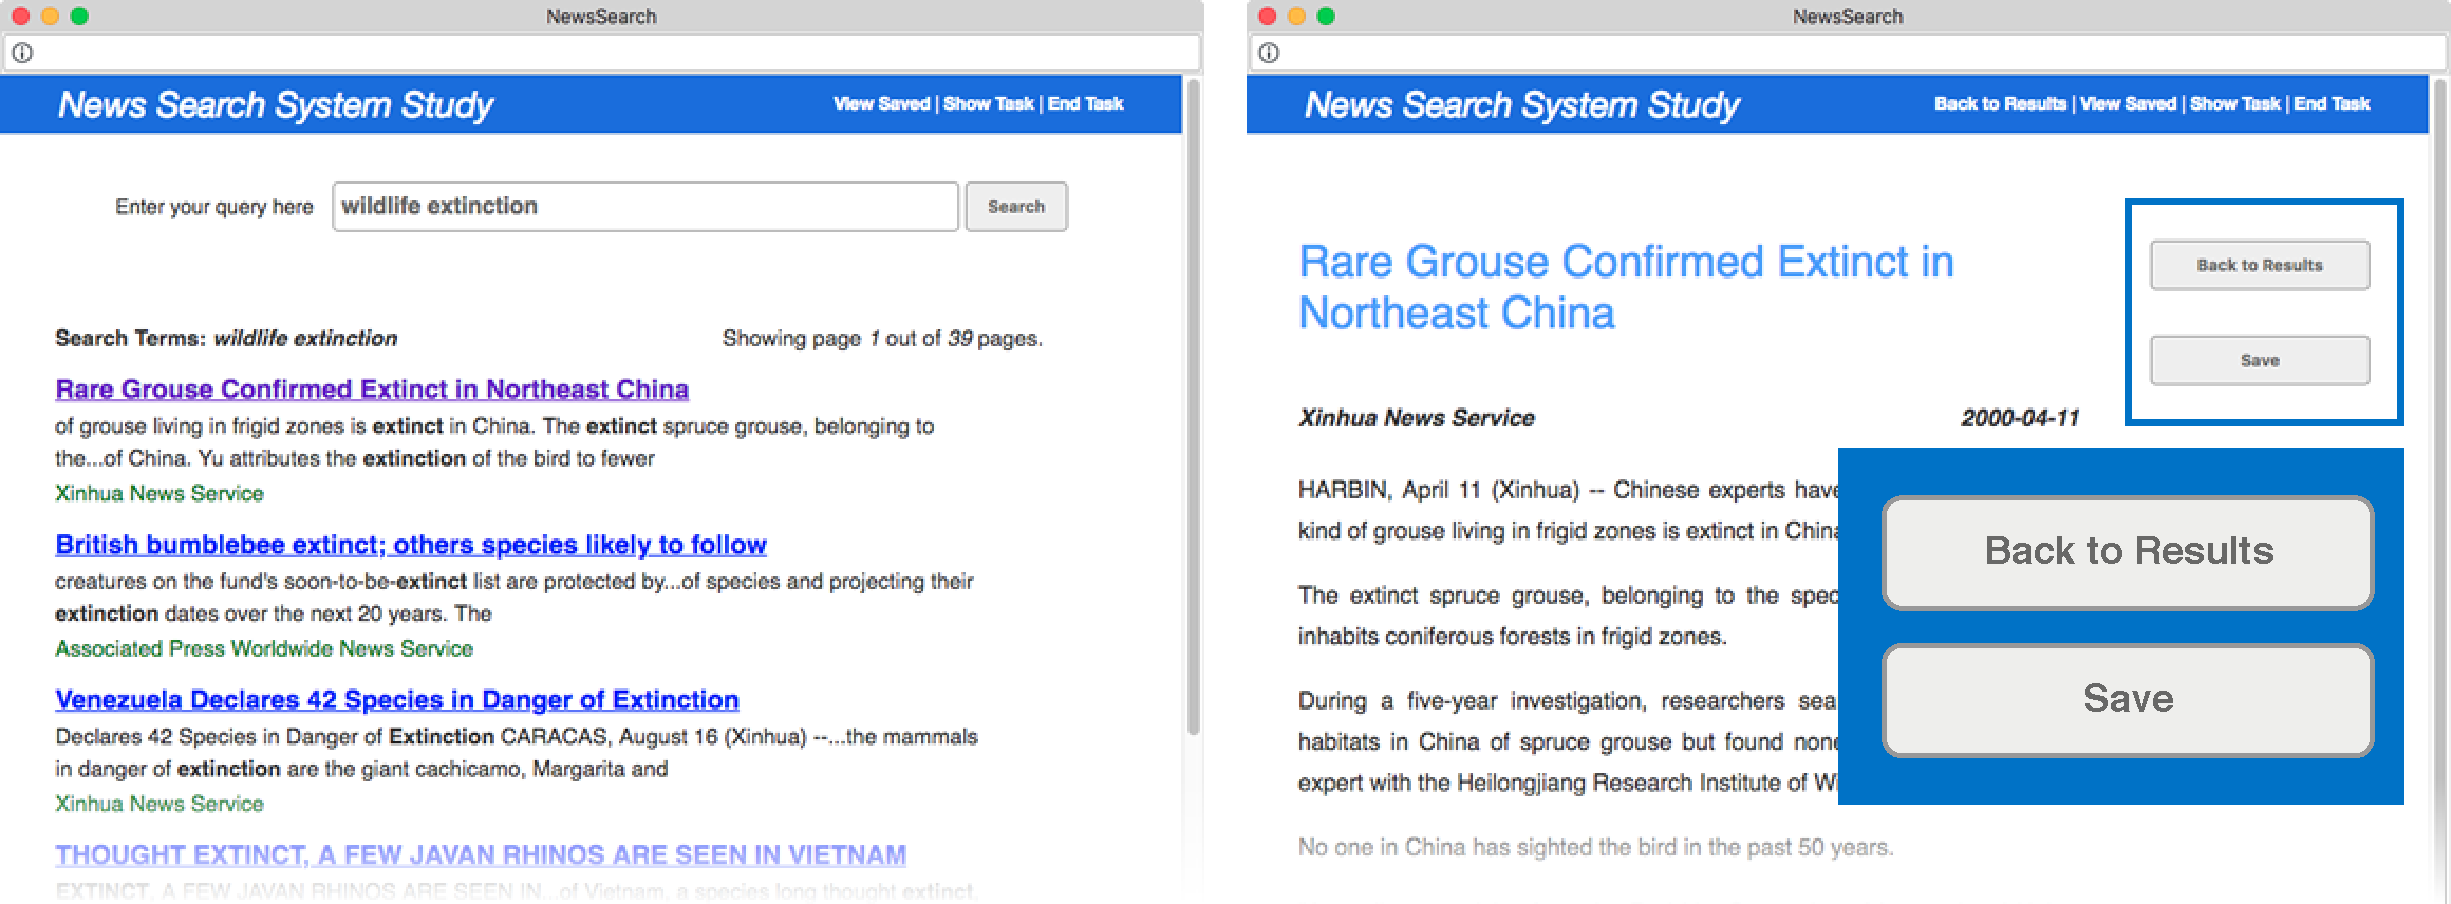
\includegraphics[width=1\textwidth]{figures/ch6-interfaces.png}}
    \caption[Example screenshots of the experimental interfaces]{Example screenshots of the basic search interface used as part of \treconomics. On the left is a screenshot of typical experimental~\gls{acr:serp} for the query \texttt{wildlife extinction}. The right shows the document view, showing the option for subjects to \texttt{Save} a document that they consider relevant to the given topic.}
    \label{fig:interfaces}
\end{figure}

\subsubsection{The Search Engine Results Page}
As can be observed from the left screenshot in Figure~\ref{fig:interfaces}, the~\gls{acr:serp} does not look all that different from a~\gls{acr:serp} on a contemporary web search engine -- sans right rail components, as we discussed previously in Section~\ref{sec:ir_background:basics}. The experimental~\gls{acr:serp} provides at the top the \emph{query box,} allowing subjects to enter their query term(s), and a button to submit their query. The \texttt{ENTER} key could also be used to submit a query.

Once submitted, results are displayed underneath the query box. The issued query is provided, along with an approximation of how many pages of results are provided to the searcher for the given query. This hints that pagination is utilised -- with 10 results per page shown. At the bottom of each~\gls{acr:serp} are links that allow the searcher to move to the next page, and vice versa.

Result summaries are shown in the accepted way -- the title, the source, and any snippet text are all provided. Given that the experiment is based upon news search, the source is the name of the newswire from which the document originates. The title was also hyperlinked -- when a subject clicked on the link, he or she would then be taken to the document view (discussed below), displaying the associated document in its entirety. Standard hyperlink colours were employed -- blue for unvisited, and purple for visited.

\subsubsection{The Document View}
The right screenshot in Figure~\ref{fig:interfaces} illustrates the document view. Particularly unexciting, the view provides the title, the document source (newswire), the date at which the document was created, and the full text of said document. On the right rail of the page, subjects were provided with two buttons -- one to return them to the originating~\gls{acr:serp}, or another to \emph{save} the document. The act of saving a document is a crucial component to both studies we discuss in this thesis. It provided us with a mechanism to determine what documents subjects thought were relevant to the given topics. Thus, this mechanism, for instance, also provided us with a means to calculate a subject's performance. Once clicked, the document was appended to a list of previously saved documents that subjects could also view.

\subsubsection{The Saved Documents View}
The third key view, as mentioned above, allowed subjects to view a list of documents that they had previously saved as relevant to the given topic. This list of documents also provided buttons, allowing subjects to change their decisions as to what constituted as a relevant document. We provided this functionality as~\gls{acr:iir} is inherently an interactive process -- a searcher \emph{learns} and develops their mental model of the given information need as more information is presented to them~\citep{ingwersen2005theturn}.

\subsection{Capturing Interactions and Survey Responses}\label{sec:csm:methodology:user:capturing}
In addition to the front-end interface provided to the subjects of each experiment, the \treconomics~framework also provided extensive logging capabilities to capture a variety of different events triggered by subjects as they performed the search tasks. This resulted in an generation of an experiment \emph{log file,} capturing the date, time, user and topic for each event that was logged. Figure~\ref{fig:log} provides an anonymised excerpt from the interaction log of the snippets user study, as discussed in Chapter~\ref{chap:snippets}. The figure illustrates the different actions that were logged from when a searcher begins interactions with the query box (\texttt{QUERY\_FOCUS}), to issuing a query (\texttt{QUERY\_ISSUED}, complete with the terms of the query), to clicking a document (\texttt{DOC\_CLICKED}), and, finally, to saving the document (or considering it relevant to the given topic, \texttt{DOC\_MARKED\_RELEVANT}). A detailed discussion of the different behavioural measures that we examined from the interaction log are detailed in Section~\ref{sec:csm:methodology:extracting}.

\begin{figure}[t!]
    \centering
    \resizebox{1\hsize}{!}{
    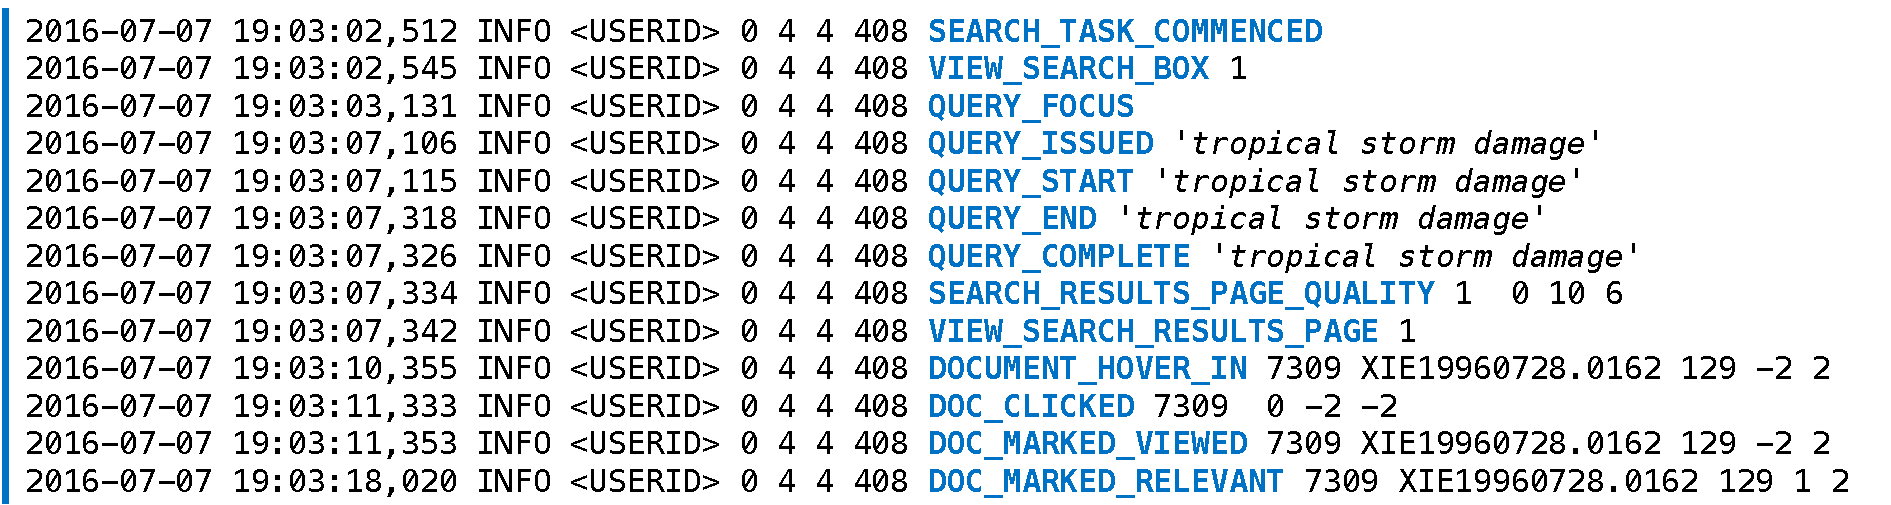
\includegraphics{figures/ch6-log.pdf}}
    \caption[Experiment log file excerpt]{An excerpt from the snippets user study, as detailed in Chapter~\ref{chap:snippets}. This example provides a sequence of interactions that were logged by the \treconomics~framework.}
    \label{fig:log}
\end{figure}

In addition to the interaction log, the \treconomics~framework also saved the responses from surveys as filled in by the subjects of each study. These were saved to a separate~\gls{acr:rdbms}, with a number of scripts subsequently created to extract and analyse the saved responses.

\subsection{Crowdsourcing Considerations}\label{sec:csm:methodology:user:crowdsourcing}
An important factor in planning any user study is the economics of collecting input from subjects. \emph{Where do the subjects come from? How do we recruit them?} A traditional, lab-based study as discussed in Section~\ref{sec:ir_background:user} typically involves a significant investment in time and monetary cost from the researchers conducting the experiment~\citep{spool2001testing}. For both user studies previously detailed, we employed a \emph{crowdsourced} approach to our experimentation. Crowdsourcing is the practice of obtaining input into a task by enlisting the services of a number of people, recruited over the Internet.

As highlighted by Zuccon et al.~\cite{zuccon2013crowdsourcing_comparisons}, crowdsourcing provides an alternative means for capturing user interactions and search behaviours. Greater volumes of data can be obtained from more heterogeneous workers at a lower cost -- all within a shorter timeframe. Of course, pitfalls of a crowdsourced approach include the possibility of workers completing tasks as efficiently as possible, or submitting their tasks without performing the requested operations~\citep{feild2010turkers}.

Despite these issues, it has been shown that there is little difference in the quality between crowdsourced and lab-based studies~\cite{zuccon2013crowdsourcing_comparisons}. Nevertheless, quality control is a major component of a well-executed crowdsourced experiment~\cite{bota2016information_cards}. Employing crowdsourcing for our two user studies, we detail in the remainder of this section the precautions that were taken during, discussing both the requirements for the subjects and their technical setup -- as well as a discussion of the crowdsourcing platform used.

\subsubsection{Platform Details}
Both studies were run over the \emph{Amazon Mechanical Turk (MTurk)} platform. Workers\footnote{In this section, a \emph{worker} refers to an individual undertaking the experiment on the MTurk platform. This term is considered interchangeable with a \emph{subject.}} from the platform each performed a single task (or, to use MTurk language, a \emph{Human Intelligence Task (HIT)}), with a single HIT corresponding to the entire experiment. This is in contrast to many HITs, where workers would typically undertake small, typically decision-based, transactions (for an example of such a study where this took place, refer to~\cite{bota2016information_cards}).

\subsubsection{Subject Requirements}
Due to the expected length that workers would take to complete the two studies\footnote{Note that two different sets of workers were used -- the studies were run at different times.}, workers who completed the study in full were reimbursed for their time with US\$9 -- greater than the hourly minimum wage set by the US federal government. Workers interested in undertaking each of the two studies were required to meet a certain minimum set of criteria to be eligible to participate. We required that workers were:

\begin{itemize}
    \item[\emph{(i)}]{from the United States;}
    \item[\emph{(ii)}]{native English speakers;}
    \item[\emph{(iii)}]{possessed a HIT acceptance rate of at least 95\%; and}
    \item[\emph{(iv)}]{had at least had 1000 prior HITs approved.}
\end{itemize}

Requiring \emph{(iii)} and \emph{(iv)} reduced the likelihood of recruiting workers who would not complete the study in a satisfactory manner. Recruits were forewarned about the length of the HIT, providing them with a chance to abandon the experiment if they felt the expected time was too long.

\subsubsection{Technical Requirements}\label{sec:csm:methodology:user:crowdsourcing:technical}
Given worker limitations, we also enforced a number of technical constraints. Workers attempting each experiment were required to have a sufficiently large computer screen to display the experimental interface without having to resort to excessive scrolling, and ensured a consistent number of result summaries would be present on different worker's screens. As such, we imposed a minimum display resolution of $1024x768$ for both studies. Conducted through a web browser, we wanted to ensure that only the controls provided by the experimental apparatus were used, meaning that the popup window that we highlighted in Section~\ref{sec:csm:methodology:user:interface} had all other browser controls disabled to the best of our ability (i.e. browser history navigation, etc.). The experimental system was tested on several major web browsers, across different operating systems. This gave us confidence that a similar experience would be had across different system configurations.

\section{Extracting User Study Data}\label{sec:csm:methodology:extracting}
As discussed in Section~\ref{sec:csm:methodology:user:capturing}, the \treconomics~framework provided the necessary infrastructure for us to log the various interactions and capture survey responses from each individual subject across the two user studies trialled. In this section, we provide details on the different aspects that we subsequently used to evaluate searcher behaviours, performance and user experience. Figure~\ref{fig:evaluation_methodology} provides a graphical illustration of how we split the various aspects we consider into four distinct categories.

The first three categories can be extracted directly from the interaction log that recorded different interactions by each subject as they progressed through the experiment. The categories we considered are listed below.

\begin{itemize}
    
    \item[]{\blueboxbold{Behavioural Measures} capture the broad interactions that take place, such as the number of documents that a searcher examined in detail.}
    \item[]{\blueboxbold{Performance} measures could be extrapolated, with aid of~\gls{acr:trec} QREL relevance judgements, to ascertain the performance of subjects.}
    \item[]{\blueboxbold{Time-Based} measures can also be derived from directly examining the interaction log, measuring the time spent between different logged interactions.}
    
\end{itemize}

In addition to these categories, we also observed a number of \blueboxbold{user experience} measures that are derived from a series of surveys that subjects were presented with as they were walked through the experimental process. In particular, as highlighted in Section~\ref{sec:csm:methodology:user:flow}, surveys were presented to subjects at a number of different stages throughout the experiment. In conjunction with the three log-based categories defined above, the user experience measures could be used to complement the empirical evidence to see whether the interactions of subjects actually correlated with their perceived experiences.

In all, the interactions -- including aspects such as clicks, and time-based measures, were used as a \emph{grounding} for our subsequent user simulations. These are discussed in Section~\ref{chap:csm:method:simulation} and derived for each experimental condition and interface trialled.

\begin{figure}[t!]
    \centering
    \resizebox{1\hsize}{!}{
    \includegraphics{figures/ch4-evaluation.pdf}}
    \caption[Examples of Evaluation Measures]{An illustration of the different types of measures that are captured, and from what sources. Interaction, time-based and performance measures are derived from the user study experiment log (with~\gls{acr:trec} QRELs used in conjunction with the interaction log to compute a subject's performance). User experience metrics are collated from a number of different surveys. Refer to Section~\ref{sec:csm:methodology:extracting} for more information.}
    \label{fig:evaluation_methodology}
\end{figure}

\subsection{Behavioural Measures}
Recorded solely from interaction log data, the basic interactions covered a large proportion of the aspects we considered in our analyses. They key behavioural measures we examined were:

\begin{itemize}
    \item{the number of \blueboxbold{queries issued};}
    \item{the number of \blueboxbold{documents viewed};}
    \item{the number of \blueboxbold{\glsplural{acr:serp} viewed}; and}
    \item{the \blueboxbold{depths} to which subjects clicked on (and hovered over), regarding the result summaries presented on the~\glsplural{acr:serp}.}
\end{itemize}

From these measures, we could then ascertain whether searcher behaviour varied when a certain condition or interface was changed -- allowing us to address questions such as \emph{whether snippet length affects the depth to which searchers examine content?} To compute depths, click and hover depths were used -- we however only report click depths in subsequent contributory chapters. The reasoning for this is discussed in Section~\ref{sec:csm:methodology:extracting:time} below. These measures were observed over each query issued by subjects.

% -- we could then take an average for each subject. We could go even further, too -- averaging over each topic, interface or condition as required to observe any notable trends in behavioural changes.

\subsection{Time-Based Measures}\label{sec:csm:methodology:extracting:time}
As discussed in Section~\ref{sec:csm:methodology:user:capturing} -- and also illustrated in Figure~\ref{fig:log} on page~\pageref{fig:log}, each logged interaction was saved with a timestamp which allowed us to determine when each event occurred.\footnote{Timestamps were saved to the nearest thousandth of a second, as per the specification of the standard Python logging framework -- refer to \url{https://docs.python.org/2/howto/logging-cookbook.html} \urlaccessed{2018-05-29} for an example of the framework in action.}. With these timestamps, we could then measure the time between two associated events, thus yielding the time taken to perform a given activity. We considered five key time-based measures across both user studies, namely:

\begin{itemize}
    \item{the time spent \blueboxbold{issuing queries};}
    \item{the time spent examining the \blueboxbold{content on~\glsplural{acr:serp}};}
    \item{the time spent examining \blueboxbold{individual result summaries};}
    \item{the time spent examining \blueboxbold{documents}; and, of course}
    \item{the summation of all of the above to yield the \blueboxbold{total session time}.}
\end{itemize}

It should be noted that in this thesis, \blueboxbold{we report all durations in seconds}. Event durations from the interaction log could be calculated in a relatively straightforward fashion. For example, the duration between the \texttt{QUERY\_FOCUS} to \texttt{QUERY\_ISSUED} events yielded the subject's query time. We of course acknowledge that in all likelihood, subjects may have considered what query to issue before focusing on the query box. However, we did not have the tools at our disposal to measure this. 

One further point worthy of note was how we computed the time spent examining each result summary. The per result summary time was approximated by taking the total time spent on a given~\gls{acr:serp}, and dividing that value by the click depth that was reached on that~\gls{acr:serp}. This was originally computed by summing up the time spent hovering over results with the subject's mouse cursor, as this was shown in prior studies to correlate strongly with the user's gaze on the screen~\citep{chen2001mouse_cursor, smucker2014judging_relevance_movements}. However, issues with network latency meant that several of the hover events were logged in the incorrect order, making such an approach unviable. Using the click depth and total~\gls{acr:serp} time provided us with an approximation with which to work with. However, the approximation also makes an assumption that subjects examined each result summary on a~\gls{acr:serp}, up until a particular depth, for an equal period of time. This was sufficient for the work in our study to ascertain whether or not a variation in the task goal or presentation of results affected search depths.

\subsection{Performance Measures}\label{sec:csm:methodology:extracting:performance}
As previously discussed, we were also able to extract a number of different performance measures from the interaction logs, too. Using the raw data from the logs, we could then, in conjunction with our set of~\gls{acr:trec} QRELs, compute a number of performances measures.\footnote{Some measures were computed with the \texttt{trec\_eval} evaluation tool, discussed in Section~\ref{sec:ir_background:basics:cranfield:trec}.} Key performance measures that we captured included:

\begin{itemize}
    \item{the \blueboxbold{overall performance of queries}, measured with \blueboxbold{P@10}; and}
    \item{\blueboxbold{interactive precision and recall} (as discussed in Section~\ref{sec:ir_background:user:evaluation:interactive_pr}), including:}
    
    \begin{itemize}
        \item{the number of documents saved (identified as relevant); and}
        \item{the number of those documents that were~\gls{acr:trec} relevant (and vice-versa).}
    \end{itemize}
\end{itemize}

\blueboxheader{Grounding Subsequent Experiments} With behavioural measures and time-based measures in particular, these could be then used to \emph{ground} subsequent experiments. Refer to Section~\ref{chap:csm:method:simulation:grounding} for further information on how this was achieved. The above measures are however sufficient for analysing how searcher behaviour changed under different contexts.

\subsection{Demographics and User Experience Surveys}\label{sec:csm:methodology:extracting:user}
A number of surveys, as discussed in Section~\ref{sec:csm:methodology:user:capturing}, were also filled out by subjects capturing a variety of information about their search experiences. While there are similarities between what is asked (refer to Chapters~\ref{chap:snippets} and~\ref{chap:diversity} for further details), we in this section provide a high-level overview of the different surveys, before examining questions that were common between the two. We break these overviews into three sections, in the order of the experimental flow detailed in Section~\ref{sec:csm:methodology:user:flow} -- demographics, pre- and post-task surveys, and post-experiment surveys.

\subsubsection{Demographics}
Details in keeping with general demographics were attained about the different subjects from this survey. These included the subject's age, gender and occupation. We also queried the subject on their highest level of professional qualification (e.g. high school, Honours, MSc or PhD). A number of questions were also asked about their perceived proficiency and approach to searching for information on the~\gls{acr:www}. Questions included how often they searched for information, what pointing device they were using (i.e. mouse, trackpad), and their preferred web search engine. Finally, given that both experiments considered news search, we asked how often the subjects searched for news articles online.

\subsubsection{Pre-Task}
Between both user studies, we asked the same questions within the pre-task survey. Subjects were provided with a short description of their search task and a topic description, providing their information need for said task. After examining the topic description, subjects were then queried on the following:

\begin{itemize}
    \item{how well they knew about the topic prior to this study;}
    \item{how relevant the topic was to their life;}
    \item{how interested they were to learn more about the topic;}
    \item{whether they had searched for information related to the topic before; and}
    \item{how difficult they felt it would be to search for information on the topic before commencing.}
\end{itemize}

Responses were provided on a five-point scale, providing the option for neutrality between the two extremes -- extremes being \emph{nothing/not at all/very difficult} to \emph{lots/very much/very easy.} Responses to these questions helped us gauge the perceived difficulty of the task, and ascertain how much background knowledge could potentially affect results.

\subsubsection{Post-Task and Post-Experiment}
Post-task and post-experiment surveys were unique to each of the two user studies. Chapters~\ref{chap:snippets} and~\ref{chap:diversity} provide further information on what questions were asked. However, the post-task surveys focused on how well the subjects thought they (and the retrieval system, under the given condition and/or interface) performed during the search task. Post-task surveys considered the experiment as a whole, asking questions about what condition and/or interface the subjects preferred, or performed more to their liking, for example.

\section{Simulating Searcher Behaviours}\label{chap:csm:method:simulation}
With the general layout and components of the two user studies explained, we now consider how we \emph{simulated searcher behaviours.} Highlighted in Section~\ref{sec:ir_background:user:simulation}, simulation provides a low-cost means for exploring a variety of different searcher strategies and configurations. In this section, we provide an overview of the general aspects of the \blueboxbold{stochastically-based} searcher simulations that we discuss the results of in subsequent chapters of this thesis. Specifically, we discuss in this section:

\begin{itemize}
    \item{how our simulations were \emph{grounded;} and}
    \item{how we instantiated the different components of the~\gls{acr:csm} defined in Chapter~\ref{chap:csm} for our simulation experiments.}
\end{itemize}

We conclude the chapter with a discussion as to how we evaluate the results from our simulations, allowing us to determine what stopping strategies offer the best overall performance and approximations of real-world searcher behaviours. This is done in consideration of the two user studies discussed in Chapters~\ref{chap:snippets} and~\ref{chap:diversity}. By grounding our simulations with data derived from the two aforementioned user studies, we can then obtain an insight into how searcher stopping behaviours varies under different contexts.

\blueboxheader{The Mean Searcher} Comparisons between simulations and real-world searcher approximations are made between the \emph{average} behaviours observed. This average behaviour is considered across each of the different experimental interfaces and conditions that we trial across the two user studies, discussed in Chapters~\ref{chap:snippets} and~\ref{chap:diversity}. This consideration: \emph{(i)} simplifies and reduces the number of simulations that are required to be run; and \emph{(ii)} provides a simple overview of how stopping behaviour varies across each interface and condition, rather than across each individual searcher.

\blueboxheader{Considering Stochastic Simulations} As eluded to above, we consider in this thesis a series of different \emph{stochastically-based} simulations that attempt to mimic searcher behaviours. Currently, a majority of research that considers the simulation of interaction are also stochastic in nature, utilising probabilistic models. For example,~\cite{carterette2011effectiveness_evaluation} simulated the interaction of users for the purposes of evaluation through a dynamic test collection. While not explicitly stated, the underlying model of their simulations followed a similar process to the~\gls{acr:csm} as described in Chapter~\ref{chap:csm}, and were instantiated with probabilistic components.~\cite{baskaya2013behavioural_factors}, as discussed in Section~\ref{sec:stopping_background:models:conceptual:simple}, developed a Markov-based model of the search process, with changes in state determined by a series of different probabilities. A similar, probabilistic browsing model was also proposed by~\cite{yilmaz2010browsing_utility}. These models considered probabilistically determining, for instance, the attractiveness of a result summary to the given information need -- something that we also utilise. We discuss this further in Section~\ref{chap:csm:method:simulation:grounding:judgements}.

\blueboxheader{The SimIIR Framework} All simulations that were run as part of this thesis were done so using the \simiir~framework, a custom built framework for the simulation of interaction within the~\gls{acr:iir} process.\footnote{\simiir~can be accessed at \url{https://github.com/leifos/simiir}. \urlaccessed{2018-05-29}} As outlined in Chapter~\ref{chap:intro}, the \simiir~framework is in effect is one of the major contributions offered by this thesis. The~\gls{acr:csm}, as outlined in Chapter~\ref{chap:csm}, is implemented within the framework and offers a high level of customisability in order to trial various different component configurations.~\cite{maxwell2016simiir} provides an overview of the framework.

\subsection{Grounding and Instantiating Simulations}\label{chap:csm:method:simulation:grounding}
Repeated many times throughout this thesis so far, the \emph{grounding} of simulations is crucial for ensuring their overall credibility~\citep{azzopardi2010workshop}. Simulations that are not properly grounded with data from real-world observations means that results would then be questionable. As such, this is an area that was taken seriously during the design of our methodology. After consideration of the~\gls{acr:csm}, we considered grounding from three key perspectives:

\begin{itemize}
    \item{the generation of pseudo-realistic \blueboxbold{queries} to issue to the underlying Whoosh search engine (refer to Section~\ref{sec:csm:methodology:collection});}
    \item{the consideration of various \blueboxbold{interaction costs}; and}
    \item{the inclusion of various \blueboxbold{interaction probabilities} for determining relevancy.}
\end{itemize}

These are considered in conjunction with our aforementioned stopping strategies (refer to Chapter~\ref{chap:strategies}), and imposed constrained on the session for each simulated searcher. The remainder of this section discusses each of the key components of our simulations, and how we instantiated them to produce realistic, credible simulations of interaction.

\subsubsection{Interaction Costs}\label{chap:csm:method:simulation:grounding:costs}
Upon the examination of the~\gls{acr:csm}, illustrated in Figure~\ref{fig:csm} on page~\pageref{fig:csm}, a number of different \emph{interaction costs} can be derived. These are costs that must be expended by searchers subscribing to the model, in order for them to successfully complete the search process. We identified five different interaction costs that searchers are faced with. The five different interaction costs are:

\begin{itemize}
    \item{the time taken to \blueboxbold{issue a query} to the underlying search engine;}
    \item{how long a searcher will spend \blueboxbold{examining a~\gls{acr:serp}}, using the time to judge whether the contents of the~\gls{acr:serp} should be examined in more detail, or abandoned altogether;}
    \item{the time taken to \blueboxbold{examine an individual result summary} in depth;}
    \item{the amount of time required to \blueboxbold{examine a document} in full; and}
    \item{the time taken for determining whether a \blueboxbold{document should be saved as relevant}.}
\end{itemize}

Costs, measured in seconds, are averaged over each different condition and interface trialled between the two different user studies discussed in Chapters~\ref{chap:snippets} and~\ref{chap:diversity}. Refer to these chapters for tables of the actual interaction costs that were extracted from the interaction log data.

\blueboxheader{Extracting Interaction Costs}
To extract interaction costs for each interface and condition, we followed the same approach as discussed in Section~\ref{sec:csm:methodology:extracting:time} for extracting time-based measures. For each of the five interaction costs, we measured the time difference between two different logged events, before computing an average. Below, we outline the key events that we used to measure each of the five interaction costs. The interaction costs are also illustrated in Figure~\ref{fig:costs}.

\begin{figure}[t!]
    \centering
    \resizebox{1\hsize}{!}{
    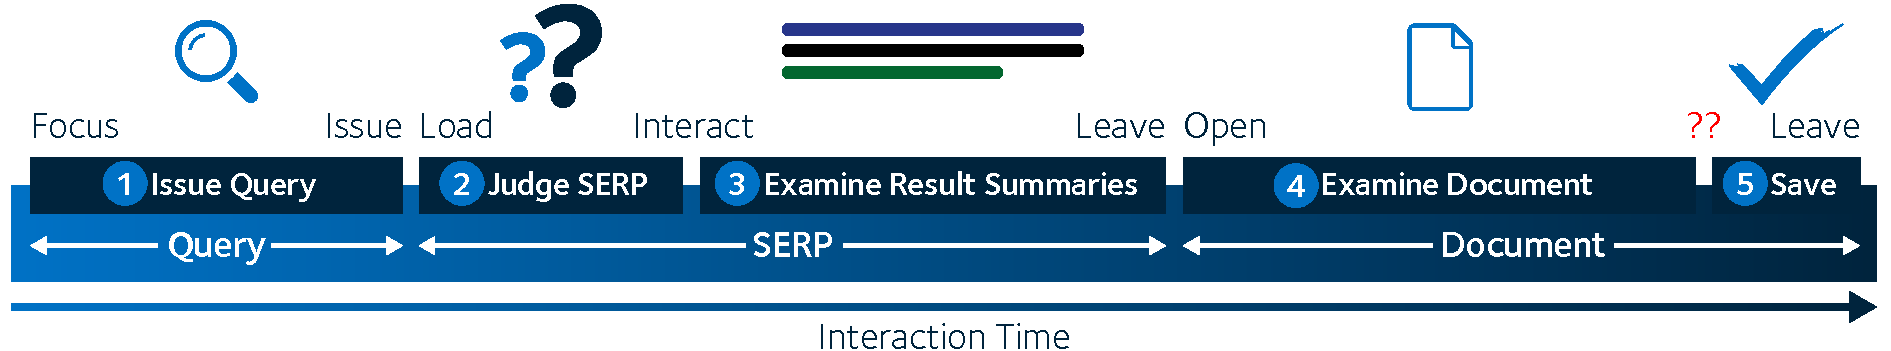
\includegraphics{figures/ch6-costs.pdf}}
    \caption[Interaction costs]{Illustration of the five interaction costs paid by searchers subscribing to the~\gls{acr:csm}. Each cost is shown with the start and end events, by which the costs were measured from the user study interaction logs. Time spent on individual components is shown in white. Refer to Section~\ref{chap:csm:method:simulation:grounding:costs} for a detailed explanation of each interaction cost considered.}
    \label{fig:costs}
\end{figure}

\begin{itemize}
    \item{\blueboxbold{1 (Querying)} As discussed in Section~\ref{sec:csm:methodology:extracting:time}, querying is measured from when the subject focused on the query box, to the point where they submitted the query.}
    \item{\blueboxbold{2 (\gls{acr:serp} Examination)} For this particular cost, we assumed that searchers would spend time judging the overall quality of the~\gls{acr:serp} from the point at which the~\gls{acr:serp} is rendered on their screen, to the point where they begin interacting with it in any way.}
    \item{\blueboxbold{3 (Result Summary Examination)} Considering the difficulties in estimating the depth to which subjects hovered over result summaries (discussed in Section~\ref{sec:csm:methodology:extracting:time}), we again used the click depth to estimate result summary examination times.}
    % This was achieved by taking the point at which a searcher began interacting with a~\gls{acr:serp}, to the point that they left it. This time was then divided by the subject's click depth for that particular~\gls{acr:serp}, yielding the estimation used.
    \item{\blueboxbold{4 (Document Examination)} This cost was determined by measuring the difference between the point at which a requested document was displayed on the subject's screen, to the point at which they left it.}
    \item{\blueboxbold{5 (Saving a Document)} \todo{The final interaction cost considered the time from which a searcher did x, to when they did y.}}
\end{itemize}

As can be seen from the discussion above, determining some interaction costs (e.g. querying) are more straightforward than others. For the~\gls{acr:serp} examination interaction and result summary interaction costs in particular, key assumptions are made considering evidence from prior studies, showing that the movements of the mouse cursor on the subject's computer screen correlate strongly with their gaze~\citep{chen2001mouse_cursor, smucker2014judging_relevance_movements}. In addition, \todo{the user interface illustrated in the right screenshot in Figure~\ref{fig:interfaces} on page~\pageref{fig:interfaces} shows that saving a document involves only the click of a button, we argue that a period of additional time must be spent to do what. As such, this is why we consider the last interaction cost listed above.}

\blueboxheader{Fixed Interaction Costs}
All simulations discussed in this thesis rely on the notion that all interaction costs are \emph{fixed} over each interface and condition trialled. This decision was primarily chosen to reduce the complexity of our simulations. By including dynamic interaction costs, this would have made the simulations themselves -- and the subsequent comparisons -- much more complex. We do acknowledge this as a limitation of our work, as a searcher should take considerably less time to judge a document consisting of two paragraphs than a document consisting of 20. We also acknowledge the existence of measures such as \emph{time-biased gain}~\citep{smucker2012tbg} that would allow for such an estimation of cost to be made.

\subsubsection{Query Generation Strategies}\label{chap:csm:method:simulation:grounding:querying}
The \emph{generation of queries} is an important aspect of any simulation of interaction. From the simplistic~\gls{acr:trec}-style model of search where a single query is issued (refer to Section~\ref{sec:stopping_background:models:conceptual:trec}), numerous studies have focused upon the issue of query generation, and how one can generate a series of pseudo-realistic queries. We discuss these prior works in Section~\ref{sec:ir_background:user:simulation}.

However, we consider a number of different \emph{querying strategies} as proposed by~\cite{keskustalo2009querying} and~\cite{baskaya2013behavioural_factors} in order to generate queries for our simulations. These strategies are considered to be \emph{idealised, prototypical} approaches to query generation, being grounded from a prior user study examining the query behaviour of subjects.\footnote{Refer to~\cite{keskustalo2009querying} for further information on the user study undertaken.}

Of the five strategies identified by the authors, we consider two in this thesis that were shown in subsequent simulations by~\cite{keskustalo2009querying} to yield the worst and best performance. The two querying strategies, named as \blueboxbold{QS1} and \blueboxbold{QS3}, are briefly explained below. We also provide an illustration of the two strategies in Figure~\ref{fig:querying}, where $Q_n$ represents query $n$ within a search session, and $t_n$ represents query term $n$ from a list of terms available to formulate queries.

\begin{figure}[t!]
    \centering
    \resizebox{1\hsize}{!}{
    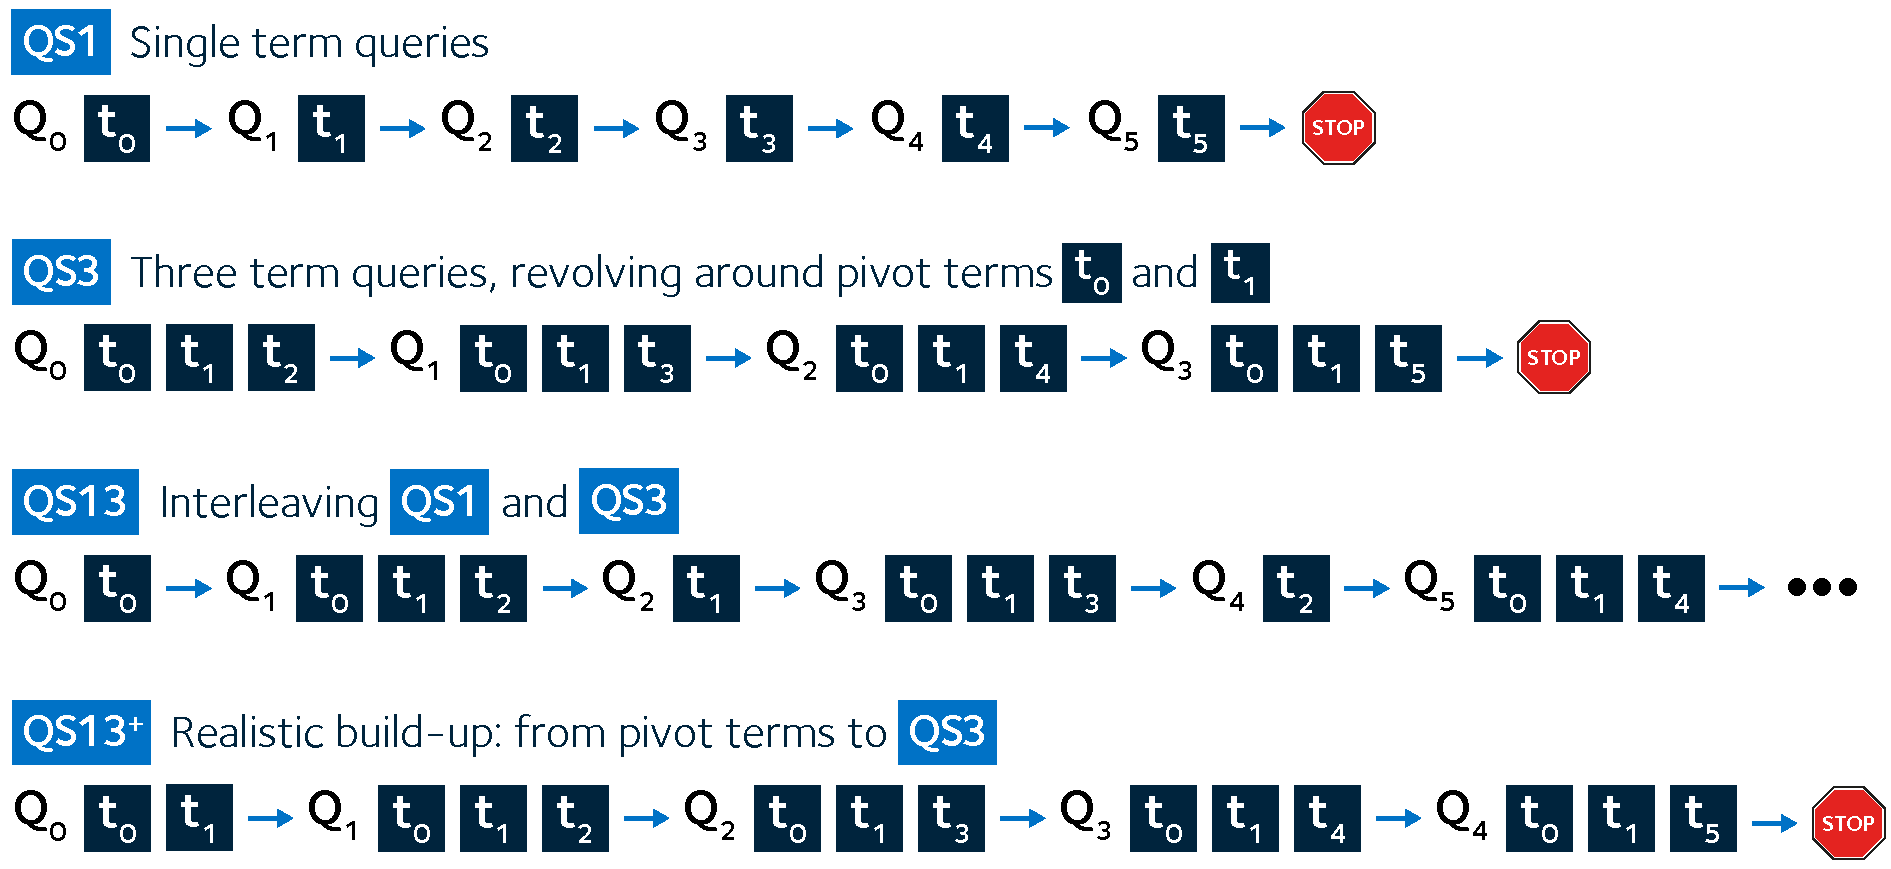
\includegraphics{figures/ch6-querying.pdf}}
    \caption[Query Strategies example]{Extensive examples of the four querying strategies used in this thesis, \blueboxbold{QS1}, \blueboxbold{QS3}, \blueboxbold{QS13} and \blueboxbold{QS13\textsuperscript{+}}. Queries are denoted by \emph{Q\textsubscript{n}}, with individual terms denoted by \darkblueboxbold{t\textsubscript{n}}. In these examples, a total of six terms are used (from \darkblueboxbold{t\textsubscript{0}} to \darkblueboxbold{t\textsubscript{5}}). Queries are separated by arrows (~
\includegraphics[height=\fontcharht\font`\d]{figures/src/arrow-blue-right.pdf}). The stop sign denotes a lack of further queries; at this point a searcher would have exhausted possible query combinations.}
    \label{fig:querying}
\end{figure}

\begin{itemize}
    \item{\blueboxbold{QS1 (Single Term)} This querying strategy generates a series of \emph{single term queries.}}
    \item{\blueboxbold{QS3 (Three Term)} This second querying strategy generates queries with two \emph{pivot} terms, and one other term. The first two terms therefore remain constant, with the third term changing for each subsequent query.}
\end{itemize}

These queries are relatively short, and are considered realistic in the sense that queries issued in real-life web search sessions consist three terms on average~\citep{keskustalo2009querying}.

With these two querying strategies in mind, we then combined them together to produce an \emph{interleaved querying strategy,} \blueboxbold{QS13}.

\begin{itemize}
    \item{\blueboxbold{QS13 (Interleaved)} With this querying strategy, queries from both \blueboxbold{QS1} and \blueboxbold{QS3} are generated, and subsequently interleaved between each other, starting with the first query from \blueboxbold{QS1}.}
\end{itemize}

Refer to Figure~\ref{fig:querying} for an example of how this strategy works. The idea behind this querying strategy is that it allows us to test the \blueboxbold{robustness} of the new~\gls{acr:serp} level stopping decision point and the various stopping strategies that we trial (our implementations of each are discussed in Sections~\ref{chap:csm:method:simulation:grounding:serp} and~\ref{chap:csm:method:simulation:grounding:stopping_strats} respectively). With~\cite{keskustalo2009querying} highlighting that \blueboxbold{QS1} yields relatively poor performance compare to~\blueboxbold{QS3}, it therefore follows that a searcher, when issuing a query generated by \blueboxbold{QS1}, will observe that the results presented are of poor quality, and thus stop at a comparatively shallower depth when compared to examining the results of queries issued by \blueboxbold{QS3}. Examining many results from a poor query is by and large a waste of the searcher's time.

Our final querying strategy, \blueboxbold{QS3\textsuperscript{+}}, is based upon the pivot term approach as seen by \blueboxbold{QS3}. Again, refer to Figure~\ref{fig:querying} for an example of how this strategy works.

\begin{itemize}
    \item{\blueboxbold{QS3\textsuperscript{+} (Realistic)} This final querying strategy builds up queries to three terms in length, using the two pivot terms as described before as a starting point.}
\end{itemize}

Previous work has shown that real-world searchers steadily build up the number of terms they used in their queries as they acquire more information. Short queries are issued initially, and the length then increases~\citep{keskustalo2009querying}. This is our rationale behind \blueboxbold{QS3\textsuperscript{+}}, and provides a more \blueboxbold{realistic} querying strategy with which to examine performance with. This is in conjunction with \blueboxbold{QS13} that allows us to test the robustness of the different stopping strategies and the~\gls{acr:serp} stopping decision point.

\blueboxheader{Reported Querying Strategies}
In this section, we introduced four different querying strategies -- two underlying strategies from the work by~\cite{keskustalo2009querying}, and two strategies based upon this prior work. The latter two allowed us to test the robustness and realism of the various simulation configurations. As such, the work in this thesis reports only on simulations that were run with \blueboxbold{QS13} and \blueboxbold{QS13\textsuperscript{+}}.

%To recap, the interleaving of good and bad queries poses a key challenge to the stopping components of the~\gls{acr:csm}: to spot a poor performing query and subsequently stop early, thus saving time.

\blueboxheader{Term List Generation}
Each of the querying strategies above are dependent upon a series of ranked terms from which queries can be created. This was achieved by first taking the \gls{acr:trec} title and description for a given topic, and creating a \emph{Maximum Likelihood Estimate (MLE)} language model (as discussed in Section~\ref{sec:ir_background:basics:models:language}), allowing us to create a probability distribution for the likelihood of a term to appear in a topic description, i.e. $p(term|topic)$. Considering our first underlying querying strategy \blueboxbold{QS1}, we could then extract a list of single terms, ranked according to $p(term|topic)$. This provided the list of terms from which queries could be generated. Our approach to pivot term-based \blueboxbold{QS3} was more complex. Taking the title terms exclusively, we then took all possible two-term combinations of the title terms, and selected the pair with the highest joint probability to act as the two pivot terms for the querying strategy. A list of candidate queries, $q$, could then be constructed by appending another term from the topic to the pivot terms (from both the topic title and description). These three term queries were then ranked according to $p(q|topic)$, yielding the final list of queries to be issued.

\subsubsection{Summary and Document Decision Making}\label{chap:csm:method:simulation:grounding:judgements}
Previously discussed in Section~\ref{chap:csm:method:simulation}, our simulations were stochastic in nature, with the decisions pertaining to the \blueboxbold{attractiveness of a result summary} \emph{(should I click this link and examine it further?)} and the \blueboxbold{relevancy of a document} to the given information need \emph{(should I save this document?)} determined through a series of different interaction probabilities. As we consider each interface and condition trialled separately, Chapters~\ref{chap:snippets} and~\ref{chap:diversity} present the interaction probabilities that were actually used within the simulations. In this section, we describe the approach used to derive them.

Like in previous studies considering the simulation of interaction -- such as those by~\cite{yilmaz2010browsing_utility} and~\cite{baskaya2013behavioural_factors}, for instance -- result summary and document decision making revolve around two key probabilities:

\begin{itemize}
    \item{the probability \blueboxbold{P(C)} of considering a given result summary on a~\gls{acr:serp} to be sufficiently attractive to \emph{`click'} and load the associated document; and}
    \item{the probability \blueboxbold{P(S)} of determining the document to be relevant to the given information need after examination, and thus \emph{saving} it.}
\end{itemize}

These are considered separately as the action of requesting a document from clicking on the associated result summary does not necessarily mean that the document \emph{is} relevant; merely, it means it appears attractive enough to examine in more detail~\citep{turpin2009summaries}. The above probabilities are broken down further with regards to~\gls{acr:trec} relevance. This entails examination of the~\gls{acr:trec} relevance judgements as discussed in Section~\ref{sec:csm:methodology:collection}, determining whether the result summary and/or document being clicked and/or saved was considered to be relevant to the given topic by the~\gls{acr:trec} assessors. As such, $P(C)$ and $P(S)$ can be split further, such that we can then determine:

\begin{itemize}
    \item{the probability that a result summary clicked is~\gls{acr:trec} relevant \blueboxbold{P(C|R)} or not \blueboxbold{P(C|N)}; and}
    \item{the probability that a document saved is~\gls{acr:trec} relevant \blueboxbold{P(S|R)} or not \blueboxbold{P(S|N)}.}
\end{itemize}

Taking these explanations, we could then take the interaction logs from the two user studies, split the interactions by the interface or condition that probabilities were to be derived for, and summate different measures -- as shown by the equation for calculating $P(C)$:

\begin{equation*}
    P(C) = \frac{|clicked_{Rel}| + |clicked_{\neg Rel}|}{|hovered_{Rel}| + |hovered_{\neg Rel}|};
\end{equation*}

and $P(S)$:

\begin{equation*}
    P(S) = \frac{|saved_{Rel}| + | saved_{\neg Rel} |}{|clicked_{Rel}| + |clicked_{\neg Rel}|}.
\end{equation*}

In the above equations, $Rel$ denotes the count for~\gls{acr:trec} relevant items, with $\neg Rel$ representing items that were not~\gls{acr:trec} relevant. Finally, $|clicked|$ represents the number of result summaries that were clicked (deemed attractive enough to examine further), $|hovered|$ denotes the number of result summaries that a subject hovered over with their mouse, with $|saved|$ denoting the number of documents that were identified as relevant, and subsequently \emph{saved.} To compute probabilities concerning~\gls{acr:trec} relevance only (i.e. $P(C|R)$ and $P(S|R)$), $\neg Rel$ elements were removed, with $Rel$ elements being removed for computing probabilities of interaction for items that were not~\gls{acr:trec} relevant (i.e. $P(C|N)$ and $P(S|N)$).

Like in Section~\ref{sec:csm:methodology:extracting:time}, the number of hovered result summaries was inferred due to issues with collecting actual hover events. To calculate the hover counts, we obtained the subject's greatest click depth for a given~\gls{acr:serp}, and summed up to that point. For example, if a subject clicked a document at a depth of $7$, the hover depth was assumed to be as such.

\blueboxheader{Stochastic Simulations}
This stochastic approach to modelling interactions provides a simple means of operationalising the components of the simulation that attempt to judge the attractiveness and relevancy of result summaries and documents, respectively.\footnote{This is not to say that stochastic approach is the only way the model such a process. For example,~\cite{maxwell2016agents} considered a \emph{deterministic} approach. A classifier was trained that then allowed a \emph{simulated agent} to deterministically decide the attractiveness of a result summary, for example.}

However, such an approach is not without limitation. By their very nature, a stochastic simulation, based upon random probabilities, will require a large number of different trials to be executed from which an \emph{average} can be formed. Each trial will potentially result in a different outcome -- perhaps, for example, with fewer documents marked in a second trial than compared to the first. This leads to a huge variance between different trials, which in turn leads to a requirement of running a large number of trials, such \emph{Monte-Carlo style simulations}~\citep{benov2016manhattan}. This in turn leads to huge increases in the amount of time required to run all simulations, as well as the computational power required.

\blueboxheader{Pre-Rolled Judgements}
To mitigate this issue, we used a series of so-called \emph{pre-rolled judgements.} This ensured that we could provide a fair comparison between configurations, whilst reducing the number of runs required to reach a point at which the simulations converged. For each document within the AQUAINT collection used, we pre-computed the various probabilities, storing them in \emph{action judgement files,} with one related to result summaries (i.e. $P(C)$), and the other related to saving documents (i.e. $P(S)$). If a document was judged to be relevant in one run, then by pre-computing these actions in advance, the same document would then be considered to be relevant in other runs.

This process was repeated ten times using different seeded values for each run. This meant that for every different simulated searcher configuration (i.e. considering stopping strategies, etc.), we ran a total of ten trials in which documents could be marked as either relevant or non-relevant. This meant, as previously mentioned, a fairer and paired comparison could be undertaken within runs. This subsequently also means that for each run, all results reported later in this thesis are the average over all ten trials. \todo{do validation simulation too}

\subsubsection{Computing Gain}\label{chap:csm:method:simulation:grounding:gain}
As searchers examine information, they \emph{gain knowledge} that helps shape their mental model of the underlying information need~\citep{nickles1995judgment}. While other works have focused upon this issue in depth, such as the work by~\cite{baskaya2013behavioural_factors}, we consider gain from a relatively simple standpoint. This keeps the complexity of our simulations manageable.

Gain is acquired when a simulated searcher, having determined to examine a document for relevance, considers it to be relevant, and subsequently \emph{saves} said document. During post-hoc analysis, we then can compute how many documents were saved and were~\gls{acr:trec} relevant. These are determined by examining the~\gls{acr:trec} relevancy judgements. The gain for the document is then simply computed as the relevancy judgement score from the~\gls{acr:trec} QRELs. Given that we utilised the~\gls{acr:trec} 2005 Robust Track~\citep{voorhees2006trec_robust}, \emph{graded relevance judgements} are used, as discussed in Section~\ref{sec:ir_background:user:evaluation:cg}. In essence, this value, when summated over all saved documents, is the \blueboxbold{Cumulative Gain (CG)} score for a simulated trial. This is discussed in more detail in Section~\ref{chap:csm:method:sim:runs}.

\blueboxheader{Gaining Elsewhere}
The means by which gain is computed in the work detailed in this thesis provides a further assumption. Gain can only be accrued from examination of a document, and subsequently saving it. This is not to say that in the real-world, searchers will not accrue gain from examination of other components, such as the result summary. This is particularly prevalent in the concept of \emph{good abandonment}~\citep{li2009good_abandonment}, where a searcher will abandon a~\gls{acr:serp} if he or she is satisfied by simply examining the information provided within result summaries, for example. We do not consider this within our simulations to simplify how gain is computed.

\subsubsection{\gls{acr:serp} Level Decision Making}\label{chap:csm:method:simulation:grounding:serp}
Previously outlined in Section~\ref{sec:csm:new_stopping}, the~\gls{acr:csm} includes an additional~\gls{acr:serp} level stopping decision point. Motivated by the \emph{information scent}\footnote{To recap, we discuss the notion of information scent in Section~\ref{sec:stopping_background:models:theoretical:ift}.} offered by a~\gls{acr:serp} (or \emph{patch}), this stopping point joins other established decision points, including snippet and session level stopping. The new decision point permits a searcher subscribing to the~\gls{acr:csm} to either \emph{enter} the~\gls{acr:serp} and begin examining result summaries in detail (if the~\gls{acr:serp}) appears to offer a good scent, or abandon the~\gls{acr:serp} if it appears to be poor, and thus save time. The remainder of this section discusses the various ways in which we implemented this new stopping decision point, allowing us to determine whether it leads to any improvements in overall search performance and better approximations to real-world searcher stopping behaviours.

\blueboxbold{Definition: Low vs. High Scent} First, we must define our interpretation of how the scent of a~\gls{acr:serp} was measured. We follow the work of~\cite{wu2014information_scent}, who stated that a page offering little or no relevant content could be considered to offer a low information scent. As such, our definition of a poor quality~\gls{acr:serp} is defined as $P@10=0.0$. We use this definition to delineate between \emph{good} and \emph{bad}~\glsplural{acr:serp} when considering interaction probabilities below.

\blueboxbold{Probability of Examination} For this new stopping decision point, we introduce the \emph{probability of examining a~\gls{acr:serp}}, or \blueboxbold{P(E)}. This determines how likely it is a searcher will \emph{enter} a~\gls{acr:serp} and begin to examine result summaries in detail. Taking this concept further, we can then consider two additional probabilities that incorporate the notion of a~\glsplural{acr:serp} information scent, yielding:

\begin{itemize}
    \item{\blueboxbold{P(E|HS)}, the probability of examining a~\gls{acr:serp} perceived to give a high information scent (i.e. a good quality~\gls{acr:serp}); and}
    \item{\blueboxbold{P(E|LS)}, the probability of examining a~\gls{acr:serp} offering what appears to be a low information scent (i.e. a poor quality~\gls{acr:serp}).}
\end{itemize}

\begin{figure}[t!]
    \centering
    \resizebox{1\hsize}{!}{
    
\includegraphics{figures/ch6-serp_probabilities.pdf}}
    \caption[Computing~\gls{acr:serp} examination probabilities]{A simple illustration highlighting how the different~\gls{acr:serp} examination costs were computed. We consider both the probability of examining~\glsplural{acr:serp} yielding both high and low information scents. Definitions are used from~\cite{wu2014information_scent} and~\cite{hassan2013serp_abandonment}.}
    \label{fig:serp_probabilities}
\end{figure}

These values were once again computed from interaction log data, derived from the two user studies discussed in Chapters~\ref{chap:snippets} and~\ref{chap:diversity}. As such, we do not report values for these probabilities here; rather, we discuss how we derived them. Refer to the specific chapters for specific values over each interface and condition trialled. Intuitively however, one would expect a searcher demonstrating competency at searching for information to know when a query is returning good results, and vice versa. As such, one would expect to see a higher probability for $P(E|HS)$ than when compared to $P(E|LS)$, and would thus provide evidence that searchers do indeed attempt to avoid low quality~\glsplural{acr:serp}.

As illustrated in Figure~\ref{fig:serp_probabilities}, we took each query issued from the interaction log, and extracted for each the $P@10$ score (as per~\cite{wu2014information_scent}). If $P@10=0.0$, the associated~\gls{acr:serp} for the query would have offered a low information scent. Conversely, if $P@10 > 0.0$, the information scent would have been considered to be high. For the interactions recorded on each~\gls{acr:serp}, we could then count the number that recorded no clicks (or no result summaries deemed to be attractive enough to examine further). We considered this as a definition of an \emph{abandoned~\gls{acr:serp}}, as used in previous work by~\cite{hassan2013serp_abandonment}. From these counts, we could then compute the probabilities of examining a~\gls{acr:serp}, as illustrated in Figure~\ref{fig:serp_probabilities}.

\blueboxbold{Considering Browser Viewport Size}
We now turn our attention to how a simulated searcher is able to make a judgement of the presented~\gls{acr:serp}. As we discussed previously in Section~\ref{sec:csm:new_stopping}, real-world searchers are able to infer the quality (and perhaps relevance) of a given page or~\gls{acr:serp} through the examination of various \emph{proximal cues}~\citep{chi2001information_scent}.

\begin{wrapfigure}[12]{r}{0.45\textwidth}
    \begin{center}
    \vspace*{-10mm}
    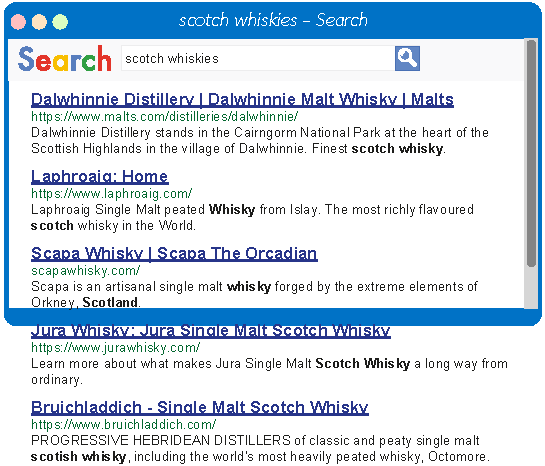
\includegraphics[width=1\textwidth]{figures/ch6-viewport.pdf}
    \end{center}
    \vspace*{-4mm}
    \caption[Viewport cutoff example]{The~\gls{acr:serp} viewport threshold. In this example, three result summaries are visible, with two not visible within the viewport. Therefore, \emph{v\textsubscript{size}=3}. Cheers!}
    \label{fig:viewport_cutoff}
\end{wrapfigure}

While we do not specifically examine different cues, instead relying on more simplistic means to operationalise the stopping decision point, we nevertheless do consider the \emph{size of the browser's viewport}. A~\gls{acr:serp} is typically larger than the viewport it is displayed within, which leads to the inclusion of scrollbars. We argue that a searcher can infer the quality of the~\gls{acr:serp} from the initial view they are presented with, and thus incorporate a \emph{viewport size} ($v_{size}$) variable in our implementations. A searcher can only judge what they can see. This variable can vary between the different interfaces we trialled -- for example, longer snippet text results in fewer result summaries being displayed in the initial view. By using a fixed-size popup window in the two user studies (as discussed in Section~\ref{sec:csm:methodology:user:interface}), we were then able to manually check the number of result summaries displayed within the popup window, and use these values to ground the new stopping decision point further.

\blueboxbold{Decision Point Implementations} We trialled three different implementations of the~\gls{acr:serp} level stopping decision point, providing us with the ability to determine the effect of incorporating it within the~\gls{acr:csm}. These are enumerated below, with an explanation of each.

\begin{itemize}
    \item{\blueboxbold{Always Examine (Baseline)} With this approach, a searcher will \emph{always enter} the~\gls{acr:serp}, and examine at least one result summary -- the exact number would be determined by the snippet level stopping strategy. This is the current state-of-the-art, and we consider this as our baseline.}
    \item{\blueboxbold{Perfect~\gls{acr:serp} Judgements} Here, a simulated searcher will only begin to examine a~\gls{acr:serp} in detail if $P@v_{size} > 0$ (considering the viewport size). If $P@v_{size} = 0$, the searcher will abandon the~\gls{acr:serp}, and proceed to the next action as dictated by the~\gls{acr:csm}. This is the upper bound in terms of performance for the stopping decision point, and is analogous to, as an example, the \emph{ideal user} of~\cite{hagen2016simulating_users}.}
    \item{\blueboxbold{Stochastic~\gls{acr:serp} Judgements} This implementation used a stochastic element to determine whether the simulated searcher should enter the~\gls{acr:serp} or not. Like above, the viewport size ($P@v_{size}$) of the~\gls{acr:serp} is computed. If the~\gls{acr:serp} is of high scent, $P(E|HS)$ is used to determine whether the searcher should enter the~\gls{acr:serp}. Conversely, if the~\gls{acr:serp} is considered to be of low scent, $P(E|LS)$ is used instead to determine the likelihood of abandonment. We considered three different sets of probabilities for the stochastic implementation.}
    
    \begin{itemize}
        \item{\blueboxbold{Average} $P(E|HS)$ and $P(E|LS)$ are estimated over all subjects of a particular interface or condition.}
        \item{\blueboxbold{Savvy} $P(E|HS)$ and $P(E|LS)$ are estimated based upon the top 15 subjects for a particular interface/condition with the lowest $P(E|LS)$.}
        \item{\blueboxbold{Na\"{i}ve} $P(E|HS)$ and $P(E|LS)$ are estimated based upon the top 15 subjects for a particular interface/condition with the highest $P(E|LS)$.}
    \end{itemize}
\end{itemize}

By considering these different approaches to implementing the new~\gls{acr:serp} level stopping decision point, we can then clearly identify whether it can offer improved performance and approximations of actual searcher stopping behaviours. \todo{Do we need to do 10 trials for the stochastic components here, too?}

\subsubsection{Snippet Level Stopping Strategies}\label{chap:csm:method:simulation:grounding:stopping_strats}
In Chapter~\ref{chap:strategies}, we detailed thirteen different stopping strategies, operationalised from various stopping heuristics and commonly used measures in~\gls{acr:ir}. Here, we once again enumerate each of the different stopping strategies, discussing what stopping threshold values that we trialled for each. For several stopping strategies, values need to be approximated from real-world interaction data (such as, for example, the~\gls{acr:rbp} patience factor). As such, many of these values were approximated from the user study detailed in Chapter~\ref{chap:snippets}, and used for all simulation experimentation. The values we ascertained were of most interest as they offer close approximations to what real-world searchers actually did.

Each of the stopping strategies, along with threshold values trialled, are enumerated below. Threshold variables are named \blueboxbold{x\textsubscript{n}}, were $n$ is the stopping strategy number. In the remainder of the thesis, we use the @ symbol to denote a particular stopping strategy with a particular threshold value, as illustrated in the front matter. For example, \stoppingstratbox{SS1-FIX}{3} represents stopping strategy \blueboxbold{SS1-FIX} with its associated threshold parameter set to $x_1=3$.

\begin{itemize}
    
    \item{For our fixed depth stopping strategy \blueboxbold{SS1-FIX}, we trialled a range values, where $x_1$ was set from $1$ to $10$ in steps of $1$, and then $15$ to $25$ in steps of $3$. This resulted in 14 separate configurations, with enough values such that a searcher would comfortably reach the time limits imposed in the study detailed in Chapter~\ref{chap:snippets}.}
    
    \item{The same range of values were used for threshold variables $x_2$ and $x_3$, for \blueboxbold{SS2-NT} and \blueboxbold{SS3-NC} respectively. These stopping strategies focused upon a searchers tolerance to non-relevance, as discussed in Section~\ref{sec:strategies:frustsat:frustration} on page~\pageref{sec:strategies:frustsat:frustration}.}
    
\end{itemize}

As alluded to in Section~\ref{sec:strategies:frustsat:frustration}, it should be noted that for \blueboxbold{SS1-FIX}, $x_1$ corresponds to the \emph{maximum depth per query,} whereas for both \blueboxbold{SS2-NT} and \blueboxbold{SS3-NC}, $x_2$ and $x_3$ represent the \emph{minimum depth per query.} For example, if $x_2=3$, a searcher would be willing to tolerate three non-relevant result summaries, finally stopping at a depth of five.

Next, we enumerate the stopping strategies considering the satisfaction, or \emph{satiation}~\citep{simon1955satiation} of a searcher.

\begin{itemize}
    
    \item{For stopping strategy \blueboxbold{SS4-SAT} concerning the number of documents a searcher should before being satisfied, find we examined a range of values for $x_4$, from $1$ to $10$ in steps of $1$.}
    
    \item{We employed the same range of values for \blueboxbold{SS13-INST}, that also considers the satisfaction of a searcher. This is considered as $T$ in INST, as discussed in Section~\ref{sec:ir_background:user:evaluation:inst}.}
    
\end{itemize}

Our combination rule then combines the frustration and satiation heuristics together to produce a strategy combining both.

\begin{itemize}
    
    \item{For \blueboxbold{SS5-COMBO}, we utilised the values used in \blueboxbold{SS1-FIX} and \blueboxbold{SS4-SAT} for frustration and satisfaction components, respectively. We trialled each possible combination of the two sets of parameter settings.}
    
\end{itemize}

Next, we consider the two stopping strategies that focus upon the \emph{difference threshold heuristic}~\citep{nickles1995judgment}, where searchers will abandon a~\gls{acr:serp} if the result summaries provided do not yield any new information.

\begin{itemize}
    
    \item{For \blueboxbold{SS6-DT}, considering the term overlap between a result summary and prior summaries, the threshold $x_6$, a range of values from $0.0$ to $1.0$ were used in steps of $0.05$. This was to explore the entire range, with the smaller the threshold, the less similar the content of the new result summary to previously examined ones.}
    
    \item{Considering \blueboxbold{SS7-DKL}, using KL-divergence, a range of values for $x_7$ from $3.0$ to $8.0$ in steps of $0.5$ were trialled. In a small-scale pilot study examining this stopping strategy over the AQUAINT document collection, a majority of values fell within this range.}
    
\end{itemize}

Next are the stopping strategy based upon optimal foraging behaviour.

\begin{itemize}
    
    \item{Following with Optimal Foraging, \blueboxbold{SS8-OFT} considers a searcher's average rate of gain. If this falls below a set threshold, then the searcher stops. We experimented with manipulating the gain threshold parameter and the number of documents first viewed before estimating the gain. For this stopping strategy, we consider only two snippets, and values for $x_8$ ranging from $0.002$ to $0.03$ in steps of $0.002$.}
    
\end{itemize}

Two result summaries were chosen for the following reason. If the first document was non-relevant, the searcher would always stop. We found that basing the estimate on two result summaries was much less sensitive and resulted in better performance. \todo{Explain this better. What about the rate of gain for different topics?}

Next, we consider the time-based stopping strategies. These values were grounded from the user study discussed in Chapter~\ref{chap:snippets}. We apply these values to the study in Chapter~\ref{chap:diversity} for a fairer comparison.

\begin{itemize}
    \item{Considering the total amount of time spent on a~\gls{acr:serp} and its associated documents, we considered for stopping strategy \blueboxbold{SS9-TT} ($x_9$) values from $30$ to $150$ seconds, in steps of $30$ seconds.}
    
    \item{Stopping after $x_{10}$ have elapsed since saving a relevant document (or the start of the search session), we for \blueboxbold{SS10-TR} considered a smaller range of values, from $10$ to $50$ seconds, in steps of $10$ seconds.}
    
    \item{The final time-based stopping strategy \blueboxbold{SS11-TCOMBO} combined together both prior time-based stopping strategies. Depending upon the quality of the~\gls{acr:serp}, a different strategy was employed. Values from \blueboxbold{SS9-TT} and \blueboxbold{SS10-TR} were used. \todo{Discuss high yield and low yield.}}
    
\end{itemize}

The final stopping strategy was based upon the~\gls{acr:rbp}~\gls{acr:ir} measure. Once again, the patience factor was grounded from the user study detailed in Section~\ref{chap:snippets}.

\begin{itemize}
    
    \item{For \blueboxbold{SS12-RBP}, we found that fitting~\gls{acr:rbp} to the user study interaction data, the patience factor ($x_{12}$) was 0.9087. As such, we trialled a range of values around this area, from $0.8$ to $0.95$ in steps of $0.05$. We also trialled $0.99$.}
    
\end{itemize}

These values, as discussed previously, were used in all simulations to provide a broad examination of the performance of each stopping strategy.

\subsubsection{Simulated Searcher Constraints}
Like in the user studies, we imposed different constrains upon the simulated searchers to keep the comparisons as fair as possible. For example, in Chapter~\ref{chap:snippets}, a session time constraint of ten minutes was imposed, as per the user study. The total time spent by a simulated searcher could be then computed, for example, by summating the interaction costs a simulated searcher had accrued up until a given point. These constraints are discussed in more detail in Chapters~\ref{chap:snippets} and~\ref{chap:diversity}.

\subsection{Simulation Runs and Evaluation}\label{chap:csm:method:sim:runs}
Having now discussed how all of the various components of the~\gls{acr:csm} and the \simiir~framework were instantiated for our simulations, we now move to a discussion of how we actually ran the simulations.

With two key research questions regarding the empirical work discussed in this thesis, we designed and executed two different sets of simulation runs in order to address them.

\begin{itemize}
    \item[]{\blueboxbold{HL-RQ3a} \emph{Given the operationalised stopping strategies outlined in Chapter~\ref{chap:strategies}, how well do simulated searchers using these strategies perform?}}
    
    \item[]{To address this question, we propose a series of \blueboxbold{performance runs} that allow us to determine the best overall level of performance that can be attained using a particular configuration of simulated searcher, via a large number of \emph{what-if} scenarios.}
    
    \item[]{\blueboxbold{HL-RQ3b} \emph{How closely do the operationalised stopping strategies compare to the stopping behaviours of real-world searchers?}}
    
    \item[]{To address this second research question, we also propose a series of \blueboxbold{comparison runs} that instead focus upon how closely different configurations of simulated searcher approximate the stopping depth of real-world searchers.}
\end{itemize}

\begin{figure}[t!]
    \centering
    \resizebox{1\hsize}{!}{
    \includegraphics{figures/ch6-sim_evaluation.pdf}}
    \caption[The wider evaluation framework]{How the two sets of simulations, represented as dark blue boxes, fit within the wider experimentation framework as discussed in this chapter. The illustration also shows what components address the two high level research questions, \blueboxbold{HL-RQ3a} and \blueboxbold{HL-RQ3b}.}
    \label{fig:sim_evaluation}
\end{figure}

These simulations fit within the wider experimental framework discussed in this chapter, illustrated in Figure~\ref{fig:sim_evaluation}. Within the figure, we can see the link between the user studies and the two sets of simulations (highlighted with \darkblueboxbold{dark blue} boxes) via the act of \emph{grounding.} The illustration also provides linkage between the simulations, and the two sets of analyses that are undertaken -- the performance analysis, addressing \blueboxbold{HL-RQ3a}, and the behaviour comparison analysis that addressing \blueboxbold{HL-RQ3b}. The performance analysis is an examination of the hundreds of different possible simulation configurations, allowing us to explore how performance varies through \emph{what-if} simulations (refer to Section~\ref{sec:ir_background:user:simulation}). In all, this process is \textbf{\color{dmax_red} repeated twice}, once per user study, as shown in the illustration. We discuss the two different sets of simulations that address research questions \blueboxbold{HL-RQ3a} and \blueboxbold{HL-RQ3b} in Sections~\ref{chap:csm:method:sim:runs:performance} and~\ref{chap:csm:method:sim:runs:comparison} respectively.

One point that has not been discussed is highlighted in Figure~\ref{fig:sim_evaluation}. When executed, the simulations, employing the \simiir~framework, are saved to a series of different interaction log files. Employing the same basic structure as the real-world interaction log file illustrated in Figure~\ref{fig:log} on page~\pageref{fig:log}, the similarity between the real-world and simulated logs allowed for the same parsing infrastructure to be used with minimal changes.

\subsubsection{Performance Runs}\label{chap:csm:method:sim:runs:performance}
Named as a series of \emph{what-if} simulations above, the performance runs instantiate the different components of the~\gls{acr:csm} and \simiir~framework as previously discussed throughout Section~\ref{chap:csm:method:simulation:grounding}. Using the grounded interaction probabilities and costs, these simulations were trialled over the 50 individual topics of the~\gls{acr:trec} 2005 Robust Track~\cite{voorhees2006trec_robust}, with queries generated via the two querying strategies outlined in Section~\ref{chap:csm:method:simulation:grounding:querying}. All in all, this provided us with a wealth of simulated interaction data from which we could calculate a series of averages over the different trials experimented. As illustrated in the example figure below, we then computed the various performance measures (unless otherwise stated) over each simulated searcher configuration, taking an average over each of the 50 topics.

\begin{figure*}[h]
    \centering
    \resizebox{1\hsize}{!}{
    \vspace*{5mm}
    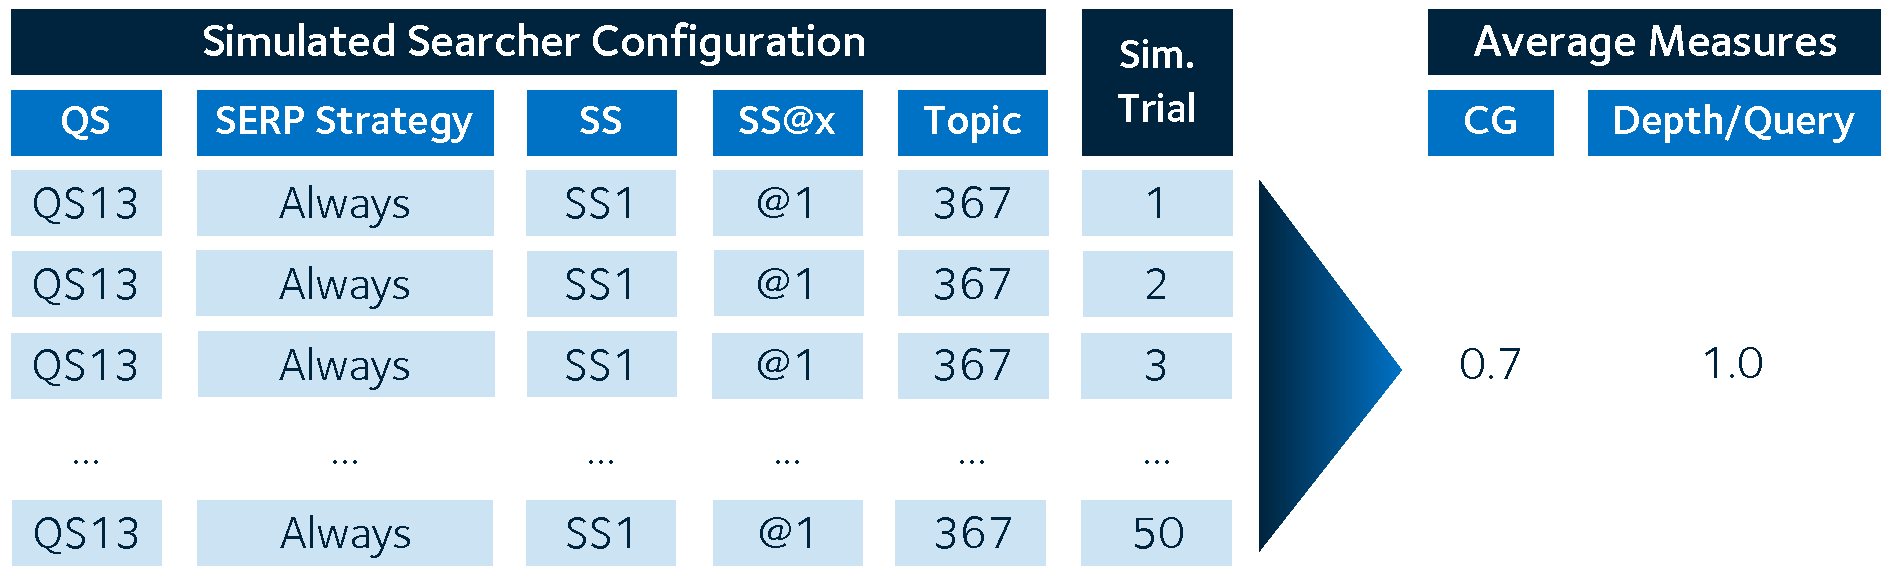
\includegraphics{figures/ch6-performance.pdf}}
    \vspace*{-6mm}
\end{figure*}

This example illustrates a single configuration of simulated searcher, using: querying strategy \blueboxbold{QS13}; the \blueboxbold{Always} (baseline)~\gls{acr:serp} examination strategy;
\stoppingstratbox{SS1-FIX}{1}; all while examining~\gls{acr:trec} topic \textnumero~303, all of which were in turn executed over ten trials. This meant that over one individual simulated search configuration, a total of $500$ simulation trials were required. Section~\ref{chap:csm:method:simulation:grounding:judgements} provides an explanation as to why these trials were required.

Given the name performance runs, we primarily examined the performance of each simulated searcher trialled. While examining the performance of queries (via the measures outlined previously in Section~\ref{sec:csm:methodology:extracting:performance}), we also examined measures illustrated in the figure above, primarily mean level of~\gls{acr:cg} attained by each simulated searcher, and the mean \blueboxbold{depth per query (D/Q)}.

\gls{acr:cg} was discussed in passing in Section~\ref{chap:csm:method:simulation:grounding:gain}. For our simulations, we consider the~\gls{acr:cg} as the amount of gain accrued over the \emph{course of a search session} -- which, by definition, can entail more than a single query. A more effective series of stopping strategies, that are better at stopping a simulated searcher examining poor quality~\glsplural{acr:serp} in any great depth, will therefore provide higher levels of~\gls{acr:cg}, but only if the queries issued offer good performance. Similarly, an effective~\gls{acr:serp} level stopping decision point implementation will stop the searcher from examining a poor~\gls{acr:serp} in the first instance, leaving more time to examine~\glsplural{acr:serp} that could potentially offer more relevant results.

The other major measure used in our performance measures was the depth per query. With this measure, performance is not measured, but rather the stopping behaviour of the simulated searchers. As shown in the illustration below, a fictional search session consists of three queries, $Q_0$, $Q_1$ and $Q_2$.

\begin{figure*}[h]
    \centering
    \resizebox{1\hsize}{!}{
    \vspace*{5mm}
    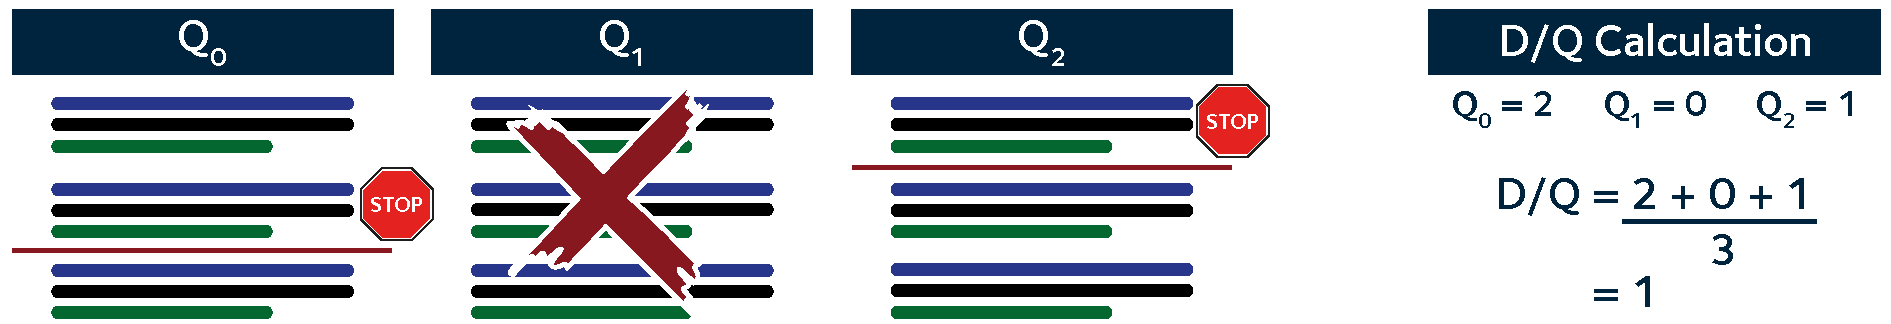
\includegraphics{figures/ch6-dq.pdf}}
    \vspace*{-6mm}
\end{figure*}

In the example, a simulated searcher examines to a depth of $2$ for $Q_0$, and a depth of $1$ for $Q_2$. The searcher does not even enter the associated~\gls{acr:serp} for $Q_1$, as the~\gls{acr:serp} level stopping decision point prevents the searcher from examining result summaries in detail. This resultant $D/Q$ for the search session is therefore $1$.

\subsubsection{Comparison Runs}\label{chap:csm:method:sim:runs:comparison}
Rather than focus upon the overall performance attained by simulated searchers under different scenarios, the second set of simulations we ran focused on comparing simulated searcher behaviours against their real-world counterparts. As such, the simulations for this set were run with minor differences in order to improve the ability for comparing the two populations of searchers -- both simulated and real-world. The first difference considered the querying component of the simulations:

\begin{itemize}
    \item{rather than considering the issuance of simulated queries via a querying strategy, we instead took the queries from the associated user study, and issued each one in turn. In effect, we \blueboxbold{replayed} all real-world queries issued.}
\end{itemize}

Following the real-world queries, we improved the realism of our simulations yet further. Queries were extracted from those issued over each individual interface and condition trialled. This also provided us with the ability to perform a direct comparison on searcher behaviour at a query level, rather than across an entire search session. However, this limited our simulations, in that:

\begin{itemize}
    \item{we considered only the \blueboxbold{four~\gls{acr:trec} topics} trialled in the user studies; the remaining 46 topics were not considered in this set of simulations.}
\end{itemize}

This was due to the fact that we only had real-world query data for the four sessions trialled in the user studies. We once again ran a simulated searcher for each different configuration, over every query issued. Ten trials were once again used, as explained in Section~\ref{chap:csm:method:simulation:grounding:judgements}.

To perform our comparisons with the real-world searchers and simulated searchers, we used the \blueboxbold{Mean Squared Error (MSE)} to compute the difference between the two. For this, our calculations were performed between the click depth of the real-world searchers over each query, and taking the simulated click depths. Simulated click depths are defined as the depth of the last document that was considered attractive enough to examine on a given simulated~\gls{acr:serp}. Considering each of simulated searcher (i.e. a combination of~\gls{acr:serp} level stopping component and snippet level stopping strategy and threshold), we could then produce a table of click depths, as provided in the example below.

\begin{figure*}[h]
    \centering
    \resizebox{1\hsize}{!}{
    \vspace*{5mm}
    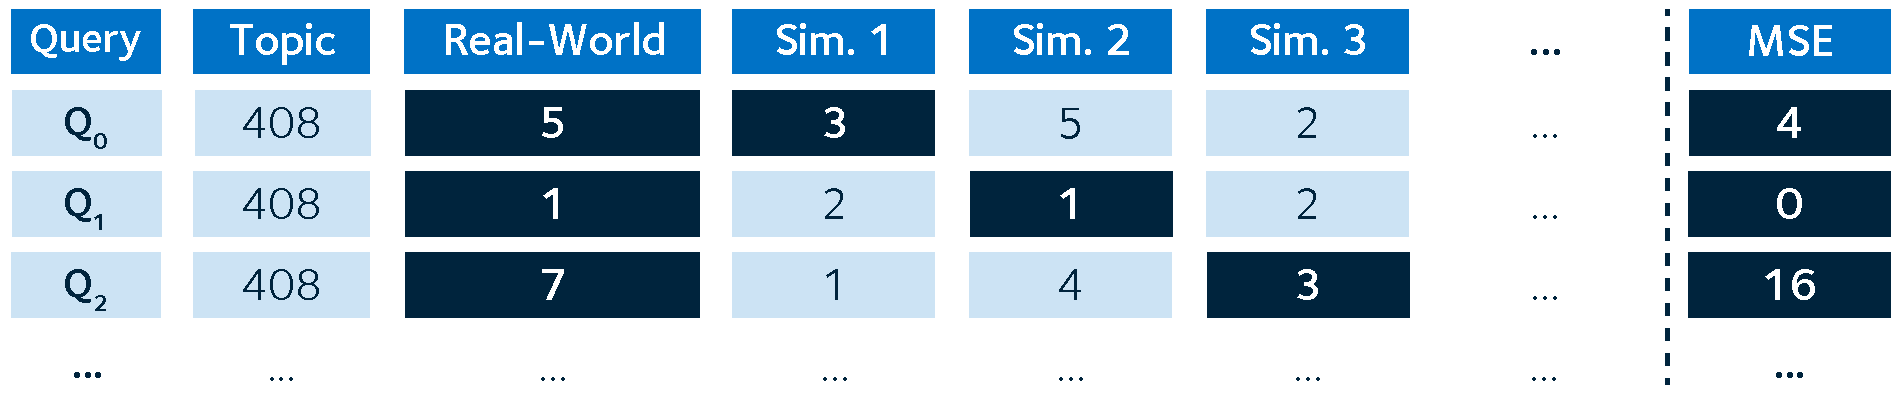
\includegraphics{figures/ch6-mse.pdf}}
    \vspace*{-6mm}
\end{figure*}

In the above, \emph{Sim. x} represents the mean value of a particular simulated searcher configuration, with the mean taken over the different simulated trials. This is the same concept as discussed previously in Section~\ref{chap:csm:method:sim:runs:performance}. For each query, the real-world click depth is shown, along with the simulated click depth from each simulated searcher trialled. The cells highlighted in light blue show what is being compared on each row -- for instance, for query $Q_0$, the real-world click depth of $5$ is compared against the \emph{Sim. 1} click depth of $3$. Considering the MSE value between the two, using the following formula:

\begin{equation*}
MSE = (\theta - \hat{\theta})^{2},
\end{equation*}

where $\theta$ denotes the real-world click depth, and $\hat{\theta}$ denotes the click depth approximation, we arrive at a MSE value of $4$. The closer the MSE value is to $0$, the better the approximation given. As such, in the above example, the compared values for $Q_1$ offer the best approximation of the actual stopping depth of the searcher. The above is just for illustration: we considered every simulated searcher, over every query. After each MSE value had been calculated, this could then be used to plot the mean depth per query across a variety of different stopping strategies. Recall, for example, that \blueboxbold{SS1-FIX} considers the stopping depth across a range of parameter values, with the parameter denoting the stopping depth. The higher this value, the greater the depth per query that will be attained. At each point, with a MSE value, we then are able to determine which stopping threshold offers the best approximation of stopping behaviour, for that particular stopping strategy.

\section{Chapter Summary}
In this chapter, we have provided an overview of the \emph{general methodology} that is used throughout the empirical work of this thesis. As we report on two separate user studies in Chapters~\ref{chap:snippets} and~\ref{chap:diversity}, this chapter provides an overview of the common approaches followed, with unique aspects discussed in the appropriate chapter.

In order to tackle the research questions posed in Section~\ref{sec:intro:rqs} on page~\pageref{sec:intro:rqs}, our general methodology was to first undertake a \blueboxbold{user study} that captured a variety of different behavioural, performance and user experience measures, as discussed in Section~\ref{sec:method:user_study}. The data derived from this user study was then used to ground a series of complex \blueboxbold{simulations of interaction}, attempting to mimic the behaviours exhibited by the real-world user study subjects. After discussing how we instantiated each of the different components of the~\gls{acr:csm} and \simiir~framework, we then concluded the chapter with a discussion on the two sets of simulation runs trialled, allowing us to address research questions \blueboxbold{HL-RQ3a} and \blueboxbold{HL-RQ3b}.

With the conclusion of this chapter, all the necessary groundwork has been laid to present the results of our user studies and simulations, which we begin in Part~\ref{part:context}.

\todo{For SS8, we need to consider the per-topic average rate of gain, I think. What about the goal-based session stopping thing? Do we need a little subsection in there, too, to explain that? We consider - time based, and - goal-based. So that is where stopping strategy 4 is used on a session-wide basis.}
    
    %!TEX TS-program = xelatex
%!TEX root = ../../maxwell2018thesis.tex

\part[Examining Searcher Stopping Behaviours]{In this part of the thesis, we present our empirical contributions, examining what happens to searcher stopping behaviours under different contexts. We then report on a number of different simulated analyses, examining our proposed stopping strategies. This also provides a means of validating the~\gls{acr:csm}.}{Examining and Simulating Searcher Stopping Behaviours}\label{part:context}
    % %!TEX TS-program = xelatex
%!TEX root = ../../maxwell2018thesis.tex

\chapter[The Effects of Snippet Lengths on Stopping Behaviour]{The Effect of Snippet Lengths on\\Stopping Behaviour}\label{chap:snippets}
    % %!TEX TS-program = xelatex
%!TEX root = ../../maxwell2018thesis.tex

\chapter[Result Diversification and Stopping Behaviour]{Result Diversification and\\Stopping Behaviour}\label{chap:diversity}
A searcher, when developing an information need, will often possess an incomplete mental model of the topic. As such, they may arrive at a retrieval system with an \emph{Anomalous State of Knowledge (ASK)}~\citep{belkin1980ask}. To address this deficiency in their mental model, a searcher will often issue a variety of different queries to explore the topic space~\citep{kelly2015search_tasks}. Often, such topics are \emph{aspectual} in nature, where an underlying goal is to find out about the different facets, dimensions or aspects\footnote{We consider aspects in this chapter, defined as `\emph{`roughly one of many possible answers to a question which the topic in effect poses''}~\citep{over1998trec}.} of the topic. An example of aspects within a topic is illustrated below, taken from TREC Robust Track~\citep{voorhees2006trec_robust} topic 347.

\begin{figure}[h]
    \centering
    \vspace{4mm}
    \resizebox{1\hsize}{!}{
    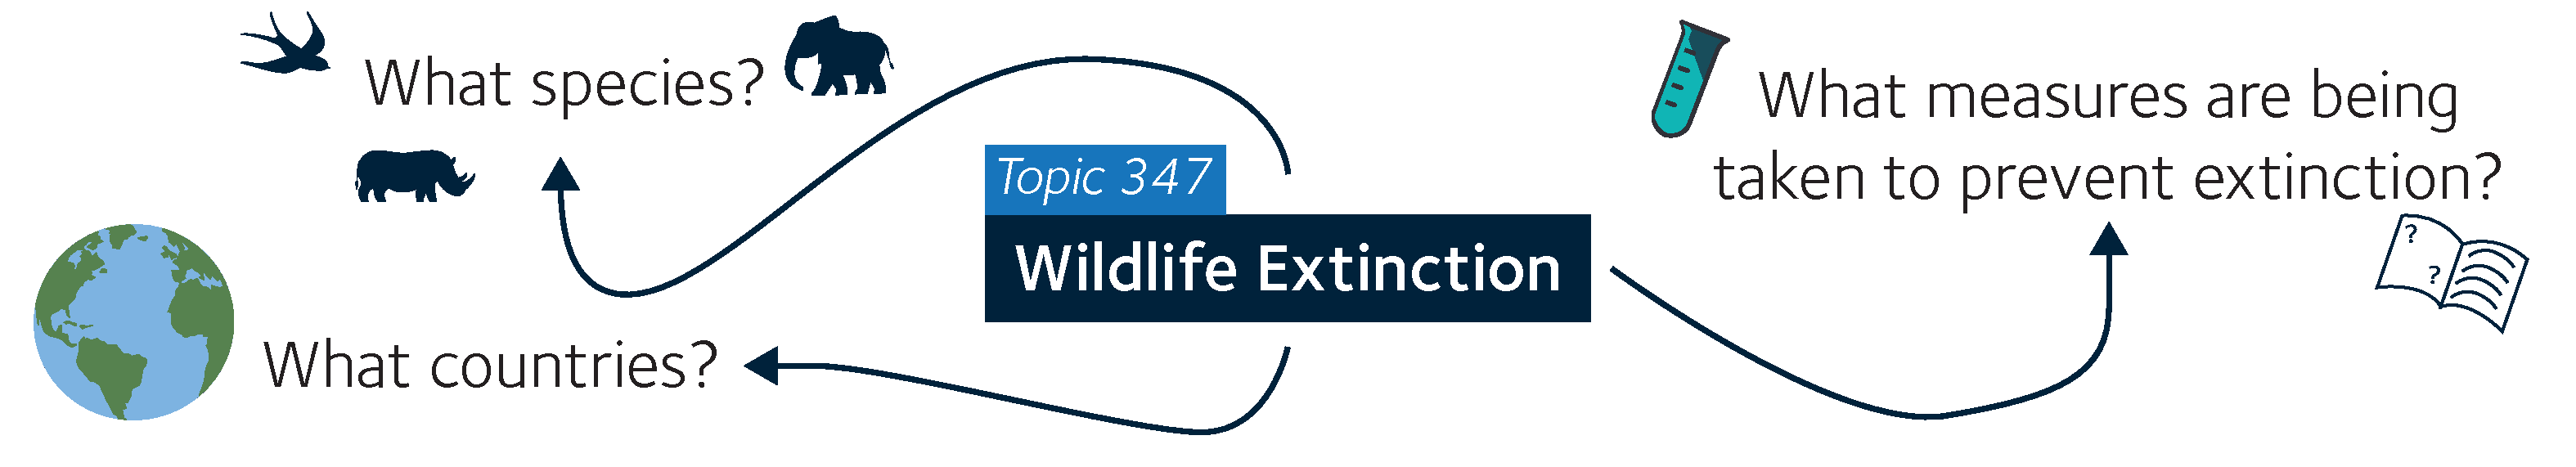
\includegraphics{figures/ch8-aspects_intro.pdf}}
    \label{fig:aspectsintro}
    \vspace{-5mm}
\end{figure}

While \emph{aspectual retrieval} has been heavily studied in the past (most prominently during the \emph{\gls{acr:trec} Interactive Tracks}~\citep{over2001trec}), there has been renewed interest in this type of search task. This is because it represents a novel context to explore the idea of \emph{``searching as learning''}~\citep{collins2017sal}. In this context, the goal of the system is to help the searcher learn about a topic~\citep{collins2017sal} -- and in doing so, the number of aspects the searcher finds provides an indication of how much they learned during the process~\citep{syed2017sal}. If the goal is to help searchers learn about a topic, then by returning results that are more diverse in nature and presenting a broader view of the topic, this \emph{should} assist searchers learn more about said topic. This reasoning suggests that employing \emph{diversification} will lead to an improved search and learning experience~\citep{syed2017sal}.

However, while there have been numerous diversification algorithms developed and proposed over the years\footnote{There are numerous examples of work on search result diversification, including measures such as \emph{Maximal Marginal Relevance (MMR)}~\citep{carbonell1998mmr}, and the \emph{xQuAD} framework~\citep{santos2010query_reformulations_diversification, santos2011intent}. Other studies in this area include works by~\cite{chen2006probabilistic_models} and~\cite{zhai2015subtopics}.}, the focus of the work reported in this chapter is on addressing the problem of intents, rather than how diversification affects complex search tasks, such as ad-hoc or aspectual retrieval. Thus, this chapter reports on:

\begin{itemize}
    \item{a user study, exploring how diversifying results (or not) affects the search behaviour and performance of searchers when undertaking different search tasks, from one of ad-hoc or aspectual retrieval (Section~\ref{sec:diversity:users}); and}
    \item{a simulated study, examining the various stopping strategies proposed in Chapter~\ref{chap:strategies}, utilising the~\gls{acr:csm}, perform under these tasks (Section~\ref{sec:diversity:simulated}).}
\end{itemize}

In particular, we use~\glsfirst{acr:ift}~\citep{pirolli1999ift} in this chapter -- outlined in Section~\ref{sec:stopping_background:models:theoretical:ift} on page~\pageref{sec:stopping_background:models:theoretical:ift} -- to derive a number of hypotheses, and thus ground our work. We begin this chapter however with a discussion of the prior work in the area, focusing upon aspectual retrieval, and a brief discussion of how~\gls{acr:ift} is used to provide us with a series of hypotheses about searcher behaviours across the different experimental conditions we trial.

\section{Background, Motivation and Hypotheses}\label{sec:diversity:background}
As discussed previously, a searcher will likely pose a varying number of queries (and~\glsplural{acr:serp}), and examine a number of documents (if any) before issuing a new query, or stopping their search altogether. The reasons for stopping are numerous. Stopping at a \emph{session level} can occur because:

\begin{itemize}
    \item{they have simply found enough information~\citep{prabha2007enough, dostert2009satisficing, hassan2013beyond_clicks};}
    \item{have run out of time~\citep{zach2005enough_is_enough}; or}
    \item{were dissatisfied with what they found~\citep{kiseleva2015serp_fails}; or}
    \item{simply gave up their search~\citep{diriye2012abandonment}.}
\end{itemize}

Numerous works have shown that different factors influence search behaviours -- this is demonstrated in Chapter~\ref{chap:snippets}, for instance, which showed how varying the length of result summaries influences behaviours. However, of particular relevance to this chapter is how different \emph{search tasks} influence a searcher's behaviours~\citep{kelly2015search_tasks}.

\subsection{Aspectual Retrieval}
An interesting search task that has not received much attention as of late is \emph{aspectual retrieval.} Aspectual retrieval is a type of search task that concerns the identification of different \emph{aspects} of a given topic. This task type differs from traditional ad-hoc retrieval in the sense that ad-hoc retrieval is concerned only with what constitutes a \emph{relevant} document to a given topic, rather than identifying relevant documents, and whether they are \emph{different} to what has been previously observed.

A relevant and different document will contain unseen aspects associated with the topic in question. With a graphical example provided at the beginning of this chapter, we now provide a further example to aid understanding. Consider the topic \emph{wildlife extinction} from the~\gls{acr:trec} 2005 Robust Track~\citep{voorhees2006trec_robust}. In an ad-hoc search task, if the searcher manages to find several documents concerning \texttt{Pandas in China}, these would all be considered relevant. However, for an aspectual retrieval task, where \emph{different} aspects must be found, the first document concerning \texttt{Pandas in China} is considered to be relevant/useful, and other aspects (in this case, the species of endangered animal) would need to be found, such as \texttt{Sumatran Rhinos in Malaysia}, \texttt{Crested Ibis in Japan}, etc.

Aspectual retrieval found significant traction in the \emph{\gls{acr:trec} Interactive Tracks}~\citep{over2001trec} from 1997-2002. The overarching goal of these tracks was to investigate searching, and an interactive task, by examining the processes involved, as well as the outcome~\citep{over2001trec}. Interaction was considered from the inaugural \emph{\gls{acr:trec}-1} in 1993~\citep{harman1993trec1}, where one group investigated interactive searching under the so-called \emph{interactive query mode} while undertaking an ad-hoc task. From \emph{\gls{acr:trec}-6} (1997) to \emph{\gls{acr:trec} 2002}, a substantial volume of research was directed towards the development of systems and search interfaces that:

\begin{itemize}
    \item{assisted searchers in exploring and retrieval various aspects of a topic, such as cluster-based and faceted interfaces that explicitly showed different aspects~\citep{mcdonald1998interactive, villa2009aspect_interface};}
    \item{provided tiles and stacks to organise documents~\citep{hearst1995tilebars, hearst1997texttiling, harper2006piling, iwata2012tilediversified}; and}
    \item{provided mechanisms to provide query suggestions that led to subjects following different search paths~\citep{kato2012query_suggestion, umemoto2016scentbar}.}
\end{itemize}

However, a disappointing conclusion from this initiative was that little difference was observed between such systems and the standard control systems (i.e. the traditional \emph{ten blue links}, as previously discussed in this thesis) -- both in terms of behaviour and performance~\citep{voorhees2005trec_book}.

As work shifted from aspectual retrieval to other areas, studies related to determining the intent of a searcher's query began to take hold, where the goal of this problem is to diversify the results retrieved with respect to the original query~\citep{rose2004understanding_user_goals}. Thus, this addresses the problem of \emph{ambiguity} for short, impoverished queries. This led to a series of diversification algorithms (and intent-aware evaluation measures), changing focus from the interface to the underlying algorithms and their evaluation measures. However, while there have been numerous studies investigating the effectiveness of diversification algorithms for the problem of query intents (e.g. one query, several possible interpretations), little work has looked at studying how such algorithms apply in the context of aspectual retrieval (e.g. one topic, many aspects). This is many due to the fact that most of these algorithms were developed \emph{after} the~\gls{acr:trec} Interactive Track finished in 2002.

Recently however, a growing interest in new, more complex and exploratory search tasks has taken hold. This is true in the aforementioned context of \emph{``searching as learning''}~\citep{collins2017sal}.~\cite{syed2017sal} hypothesised that diversifying the results presented to searchers would improve their learning efficiency, and that this would be observed by a change in vocabulary expressed in their queries. This work reported in this chapter motivates our interest examining the effects of diversification when considering the task of aspectual retrieval, where a searcher needs to learn about different aspects of a topic. To ground our work, we now consider how search behaviours are likely to be changed by generating a series of hypotheses from~\gls{acr:ift}.

\subsection{Tasks and Information Foraging Theory}\label{sec:diversity:background:tasks}
To motivate our hypotheses for this chapter, we can draw upon~\gls{acr:ift}~\citep{pirolli1999ift}, and the \emph{patch model} in particular, to ground our research and provide insights into how search behaviours may change. The patch model, as detailed in Section~\ref{sec:stopping_background:models:theoretical:ift}, provides a mechanism for predicting how long foragers will stay in a patch before moving onwards to the next. Using the established approach discussed previously -- where moving between patches is akin to issuing a new query, while staying within a patch considered examining a~\gls{acr:serp} and linked documents -- we can then make a series of predictions as to how searchers will behave under different experimental conditions.

\begin{figure}[t!]
    \centering
    \resizebox{1\hsize}{!}{
    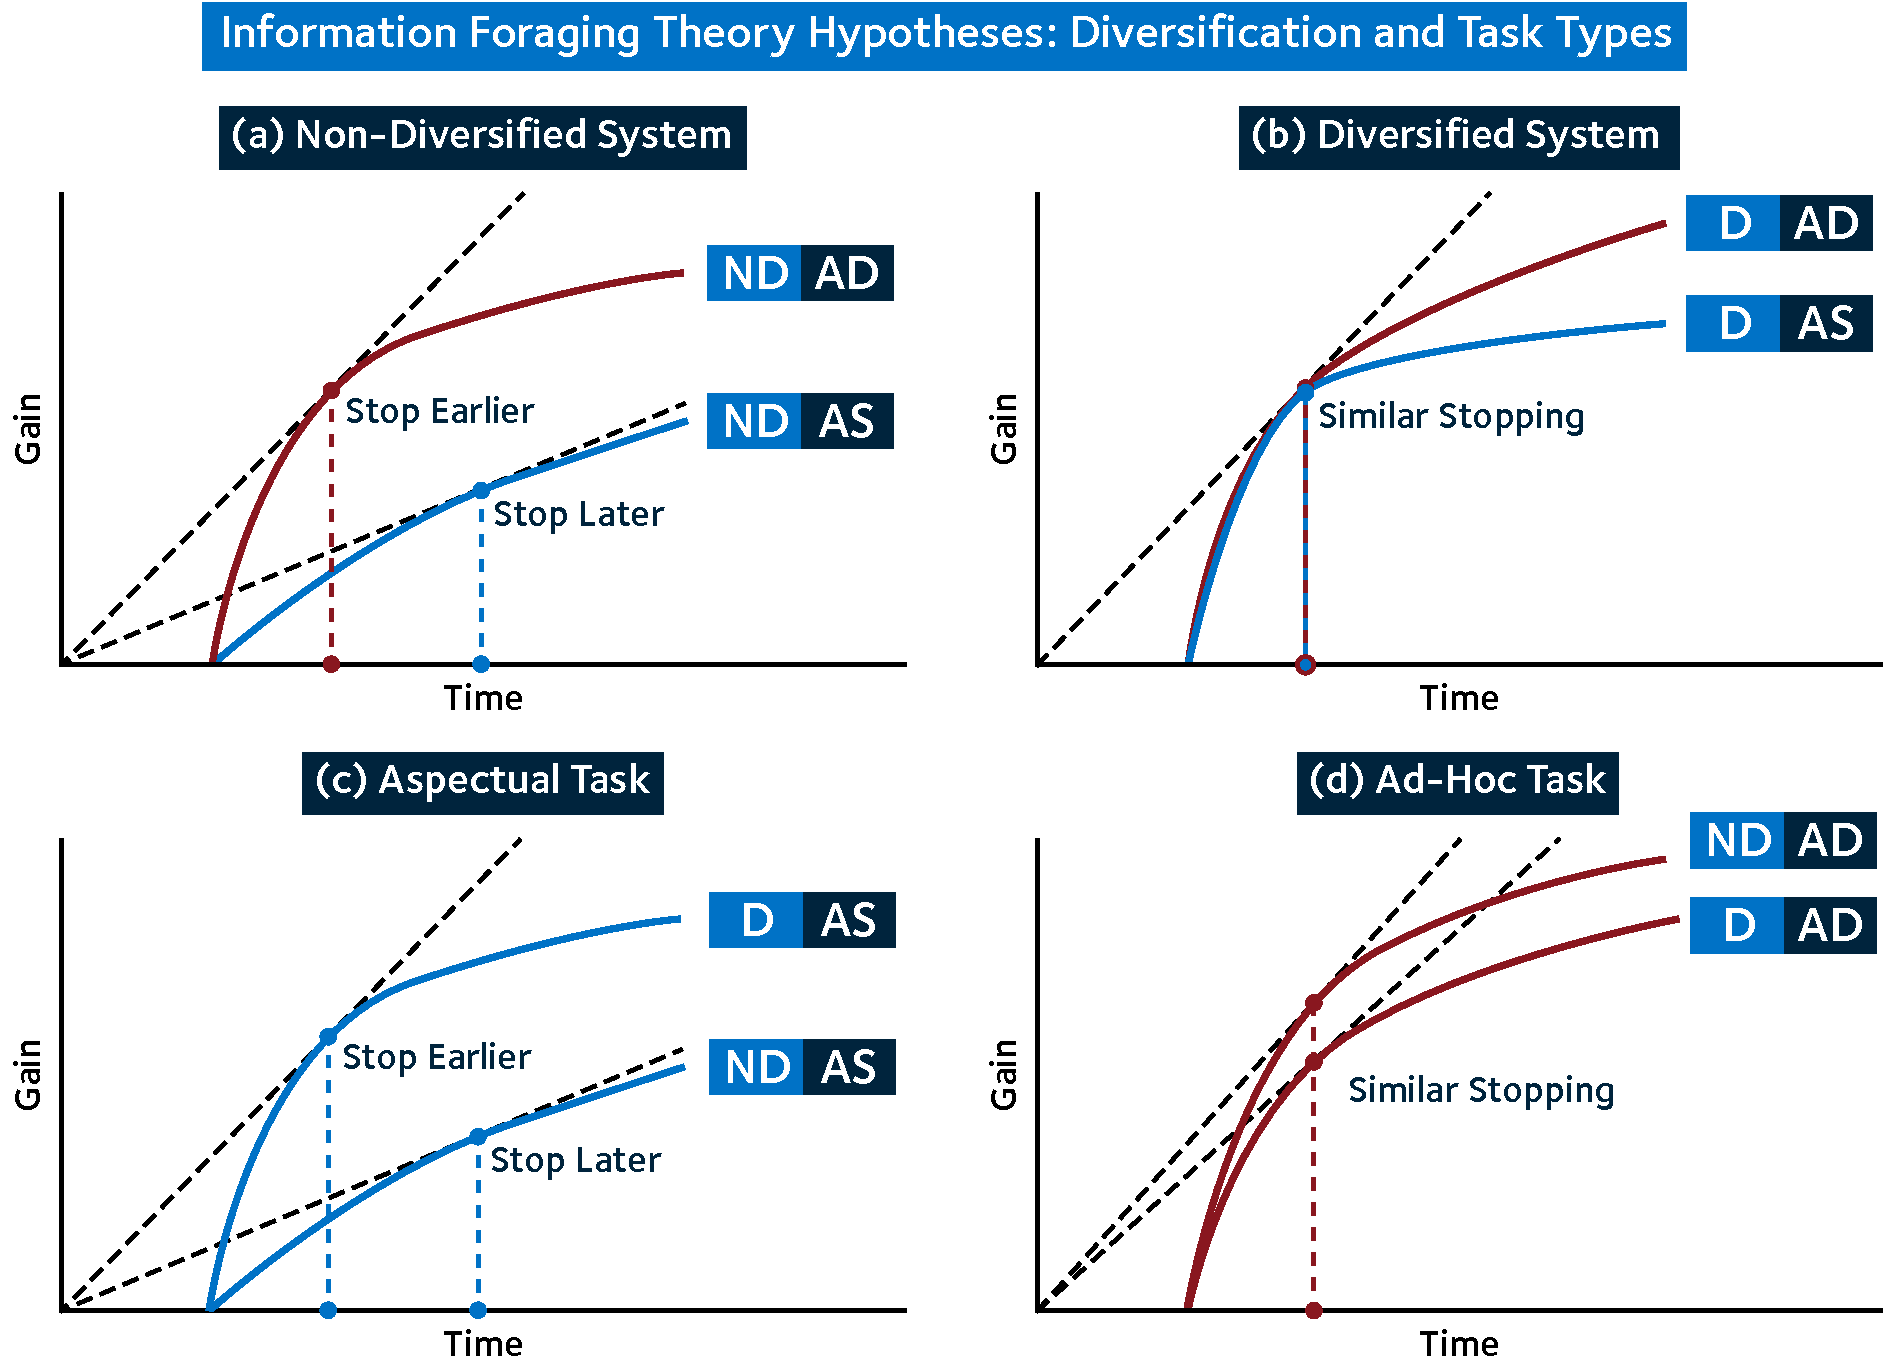
\includegraphics{figures/ch8-ift_theory_plots.pdf}}
    \caption[\gls{acr:ift} and Diversification: Hypothesis Illustrations]{Graphical illustrations of the hypotheses motivated by~\gls{acr:ift}, with each plot showing how stopping behaviour is likely to be affected when using a system that \emph{(a)} diversifies results and \emph{(b)} doesn't, and over \emph{(c)} aspectual and \emph{(d)} ad-hoc tasks. Section~\ref{sec:diversity:users:method} enumerates the four different experimental conditions shown here, such as \dualbluebox{ND}{AD} for instance.}
    \label{fig:ift_theory}
\end{figure}

These predictions are graphically illustrated in the four plots shown in Figure~\ref{fig:ift_theory} -- over a diversified \blueboxbold{D} and non-diversified \blueboxbold{ND} system, with ad-hoc \darkblueboxbold{AD} and aspectual \darkblueboxbold{AS} retrieval tasks.\footnote{The system and task are combined together to produce a complete condition, such as \dualbluebox{ND}{AD} representing a non-diversified system, with an ad-hoc retrieval task.} Gain curves for each of the four conditions are shown. In the top left plot~\ref{fig:ift_theory} \emph{(a)}, where a non-diversified system is being used, the gain curve for the ad-hoc retrieval task is higher, as any relevant document contributes to the searcher's gain. Conversely, the gain curve is lower for the aspectual retrieval task. This is because similar relevant documents would not contribute to the overall level of gain experienced by the searcher.

From~\gls{acr:ift}, the optimal stopping point would be different between the two tasks. As we discussed in~\ref{sec:stopping_background:models:theoretical:ift}, we can graphically find this point by drawing a line from the origin to the tangent of the gain curve. Red and blue dots indicate the optimal stopping points for ad-hoc and aspectual retrieval, respectively.~\gls{acr:ift} therefore suggests that with a non-diversified system, searchers will examine more documents per query for aspectual retrieval tasks when compared to ad-hoc tasks.
Discuss IFT, and then lead onto the hypotheses.

Plot~\ref{fig:ift_theory} \emph{(b)} illustrates gain curves where a diversified system would be used, with gain curves for ad-hoc and aspectual retrieval being similar in nature. This is because the diversified should bring relevant but different documents closer to the top of the rankings earlier. In the case of ad-hoc retrieval, these relevant (even if different) documents would still contribute to the overall level of gain. For aspectual retrieval, relevant and different documents will also contribute to the overall level of gain experienced by the searchers -- up to the point where the documents become similar to previously examined material. Therefore,~\gls{acr:ift} appears to suggest that similar stopping behaviours would be observed when searchers use a diversified search system.

Plot~\ref{fig:ift_theory} \emph{(c)} shows the predicted stopping behaviour for the aspectual retrieval task, where we have plotted the aspectual gain curves from the system plots \emph{(a)} and \emph{(b).} Interestingly,~\gls{acr:ift} suggests that searchers will stop sooner when using the diversified system. As such, if searching for the same length of time, searchers would thus issue more queries. Finally plot~\ref{fig:ift_theory} \emph{(d)} shows the predicted stopping behaviour for the ad-hoc retrieval task, where again we plot the curves from the respective systems in plots \emph{(a)} and \emph{(b).} Note that here, the gain curve for the diversified system may be a little lower as some irrelevant but different material may bubble up the rankings. However, as can be seen, we expect little difference overall between the two systems, and so we hypothesise that the two levels of gain (and searcher behaviours) will be approximately be the same. Consequently,~\gls{acr:ift} suggests that there will be little difference in terms of stopping behaviours between the two systems with ad-hoc retrieval tasks.

However, we found~\gls{acr:ift} to counter our intuitions as to how searchers would \emph{behave.} When using a standard, non-diversified retrieval system, our intuition suggests that since the aspectual retrieval task is rather exploratory, searchers are then more likely to issue more queries as they learn about the topic, and try to explore efforts made by different countries to protect different specifies, for example.~\cite{kelly2015search_tasks} for example showed that more complex search tasks required a greater number of queries. If a searcher submits a query that retrieves relevant material such as \texttt{protecting Pandas in China}, then one would expect them to only select one or two examples, rather than many more. In the case of ad-hoc topic retrieval, we would \emph{intuitively} expected that searchers would issue fewer queries and examine more documents. This is because they don't need to find multiple aspects. However, when using a diversified system, which attempts to promote different aspects of a given topic, we would \emph{intuitively} expect that the behaviour of searchers would change, such that when undertaking aspectual retrieval, they would issue fewer queries and examine a greater number of documents per query.

\subsubsection{Hypotheses}\label{sec:diversity:background:tasks:hypotheses}
From the plots and descriptions provided above, we can formulate a number of different hypotheses relating to the expected searcher behaviours under different contexts.

Under aspectual retrieval search tasks, using a diversified system will lead to:
\begin{itemize}
    \item{\blueboxbold{H1} fewer documents examined per query; and}
    \item{\blueboxbold{H2a} more queries issued; or}
    \item{\blueboxbold{H2b} a decrease in the task completion time.}
\end{itemize}

With ad-hoc retrieval tasks, diversification will lead to:
\begin{itemize}
    \item{\blueboxbold{H3} no difference in the number of documents examined; and}
    \item{\blueboxbold{H4} no difference in the number of queries issued.}
\end{itemize}

While the contradiction between~\gls{acr:ift} and our intuitions provides an ulterior hypothesis. In addition, given the findings demonstrated by~\cite{syed2017sal}, we also hypothesis that diversification will lead to a greater awareness of the topic, regardless of the task put forward, as more aspects will be encountered and found.

\section{Diversifying Search Results}\label{sec:diversity:users}
Following on from the motivation and experimental,~\gls{acr:ift}-based hypotheses outlined above, this section discusses the user study that was undertaken in order to examine the aforementioned hypotheses. As per our general user study methodology discussed previously in Section~\ref{sec:method:user_study}, we conducted a within-subjects experiment, with the specific details for this study discussed in Section~\ref{sec:diversity:users:method} below.

The primary research question for this user study is as follows.

\begin{itemize}
    \item{\blueboxbold{RQ} How does diversification affect the search performance and behaviour when searchers under ad-hoc and aspectual retrieval tasks?}
\end{itemize}

This research question is addressed in tandem with the hypotheses put forward above in Section~\ref{sec:diversity:background:tasks:hypotheses}. Below, we now discuss the specific details for this user study, before discussing the results, with an emphasis on stopping behaviours, and whether or not the empirical evidence supports our hypotheses.

\subsection{Methodology}\label{sec:diversity:users:method}
As discussed above, this section outlines the specific details of this user study, and is to be considered in conjunction with the general user study methodology we employ, outlined in Section~\ref{sec:method:user_study}. The same basic retrieval system employing BM25, document corpus and topics were used as previously discussed.

The within-subjects study considers two key factors: the \emph{system} and the \emph{task.} For the system factor, our baseline control system was based upon BM25 (i.e. no diversification), and a diversified system. The details of our diversification approach are discussed in Section~\ref{sec:diversity:users:diversifying}. For the task factor, we used the standard ad-hoc retrieval task, and compared this against the aspectual retrieval task. This resulted in a $2x2$ factorial design. Each subject who took part in this study therefore completed four different search tasks, one in each of the four conditions (as we enumerate below). Each of the conditions were assigned using a Latin square rotation to minimise any ordering effects. The conditions listed below are also used in Section~\ref{sec:diversity:background:tasks} when explaining the plots supporting our hypotheses.

The first two conditions consider a non-diversified retrieval system \blueboxbold{ND} (i.e. BM25, our baseline).

\begin{itemize}
    \item{\dualbluebox{ND}{AS} A non-diversified system, with an aspectual retrieval task.}
    \item{\dualbluebox{ND}{AD} A non-diversified system, with an ad-hoc retrieval task.}
\end{itemize}

Our second set of conditions therefore consider a diversified system \blueboxbold{D}, using BM25 as a baseline and an additional diversifying component, as we discuss later in Section~\ref{sec:diversity:users:diversifying}.

\begin{itemize}
    \item{\dualbluebox{D}{AS} A diversified system, with an aspectual retrieval task.}
    \item{\dualbluebox{D}{AD} A diversified system, with an ad-hoc retrieval task.}
\end{itemize}

With non-diversifying and diversifying systems, we developed different sets of branding for each system, each with their own distinct colour scheme, name and logo. This was to assist searchers in differentiating between the two. First, in terms of branding, we created two fictional search engine names:

\begin{itemize}
    \item{\blueboxbold{YoYo Search}, representing the non-diversified \blueboxbold{ND} system; and}
    \item{\blueboxbold{Hula Search}, representing the diversified \blueboxbold{D} system.}
\end{itemize}

\begin{figure}[t!]
    \centering
    \resizebox{1\hsize}{!}{
    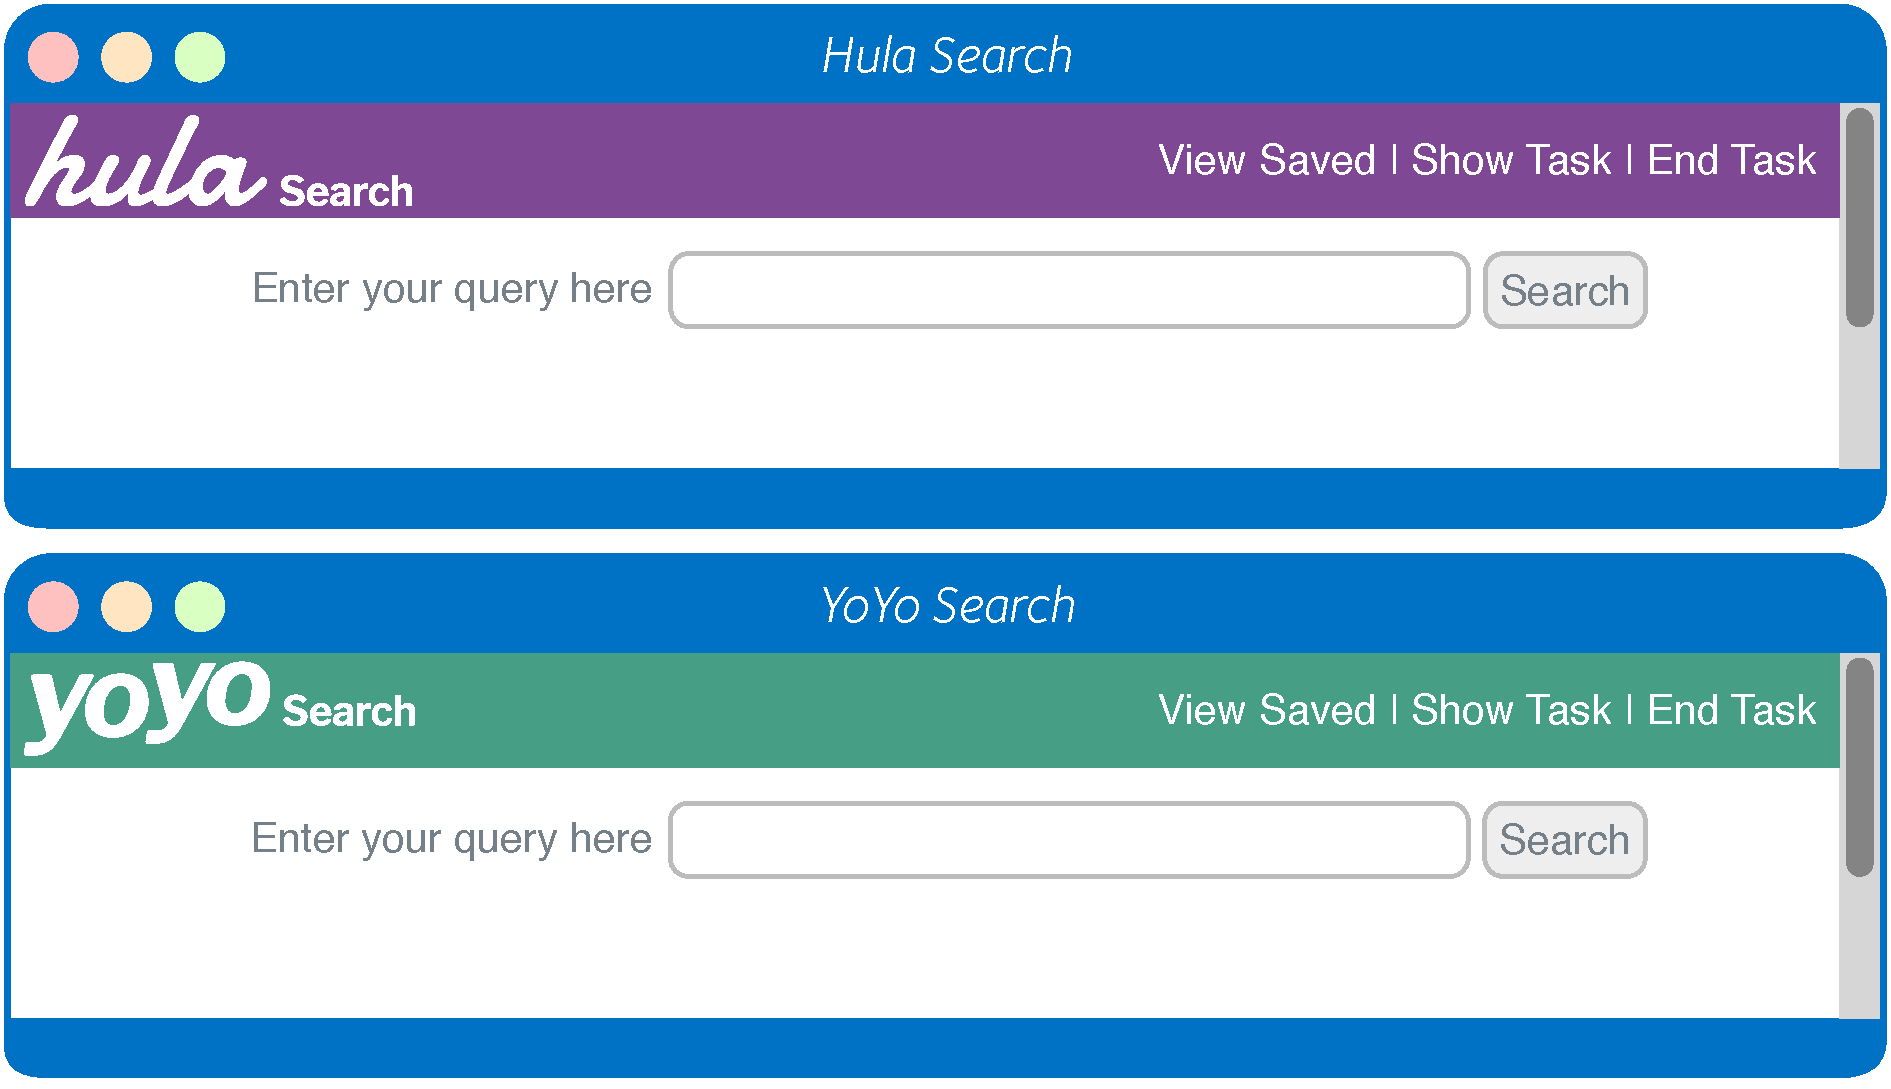
\includegraphics{figures/ch8-interface_headers.pdf}}
    \caption[Diversity user study interface mockups]{Mockups of the two names and colour schemes used to differentiate between the two experimental systems used in this user study. \emph{Hula Search} and \emph{YoYo Search} represented the non-diversified and diversified systems respectively. Refer to Section~\ref{sec:diversity:users:method} for more information.}
    \label{fig:interface_headers}
\end{figure}

These names were chosen as they were not associated with any major search engine (to the best of our knowledge), nor did they imply that one of the systems performed better than the other. Colour schemes were chosen to provide the greatest different in visual appearance to those with colourblindness.\footnote{Two of the more common variants of colourblindness, \emph{protanopia} and \emph{deuteranopia,} were both considered.} This was to ensure that subjects could later on indicate what one of the two systems that they preferred, for example. Note that only the colour schemes and logos varied -- the same basic interface layout as previously discussed in Section~\ref{sec:csm:methodology:user:interface} was employed. Figure~\ref{fig:interface_headers} demonstrates the two different colour schemes and logos for the two systems.

For the practice task, it should be noted that the standard, blue colour scheme as shown in Figure~\ref{fig:interfaces} on page~\pageref{fig:interfaces} was used. This is the same colour scheme as used in the user study reported in Chapter~\ref{chap:snippets}. A standard \texttt{News Search System Study} title was also used in place of any logos. This decision was taken to remove any impact that incorporating an individual system's colour scheme in the practice task would have on searcher behaviour or perceptions. All subjects used the \dualbluebox{ND}{AS} system and task for the practice task.

\subsubsection{Search Tasks}
As we discussed in Section~\ref{sec:csm:methodology:user:flow}, subjects were grounded by instructing them to imagine that they were newspaper reports. As such, they were required to gather documents to write stories about the four topics they searched for. Given each topic, each subject was then further instructed for this study to focus on a different criterion.

\begin{itemize}
    \item{For \blueboxbold{ad-hoc retrieval} tasks, subjects were simply instructed to find documents that were \emph{relevant} to the topic provided.}
    \item{For \blueboxbold{aspectual retrieval} tasks, subjects were instructed not only to find documents that were relevant, but also discussed \emph{different} aspects of the provided topic.}
\end{itemize}

For example, take the \emph{Airport Security} topic (refer to Section~\ref{sec:csm:methodology:collection}). Under an ad-hoc retrieval task, subjects were required to learn about the efforts taken by international airports to better screen passengers and their carry-on luggage. For aspectual retrieval tasks, subjects were also asked to find relevant documents that are different, mentioning \emph{new airports.} Thus, subjects were explicitly instructed to find a number of examples from different airports, as opposed to a similar or the same example based in the same airport multiple times.

\blueboxheader{Task Goal}
Instead of imposing a time limit as per the user study reported previously in Chapter~\ref{chap:snippets}, we instead instructed subjects to find and save at least four useful documents -- with useful denoted as being relevant, or relevant and different, depending upon the given task. Refer to the following section for details on the reasons behind selecting this value.

\subsubsection{Crowdsourced Subjects and Controls}
Subjects undertaking the user study were informed that from a small-scale pilot study, it would take approximately 7-10 minutes of their time to find at least four useful documents per task. Combining everything together, this meant that the entire experiment would take approximately 40-50 minutes of their time. Since we did not impose any time constrains on how long subjects searched for, we instead established accuracy based control. We informed subjects that their accuracy in identifying useful material would be examined, and that they were required to find four useful documents with at least $50\%$ accuracy (based upon~\gls{acr:trec} relevance judgements as the gold standard). Using data from the prior user study reported in Chapter~\ref{chap:snippets}, the accuracy of those subjects was between $25\%$ and $40\%$ on average, depending upon the topic. While we stipulated a higher accuracy, this was to motivate subjects to work diligently.

In all, a total of $64$ subjects performed the the experiments that complied with the~\gls{acr:mturk} recruiting constraints we imposed. However, a total of $13$ were omitted from this figure because they either:

\begin{itemize}
    \item{failed to complete all the search tasks (a total of five subjects were removed);}
    \item{failed to mark at least four documents (two subjects); or}
    \item{spent less than two minutes per task, and failed to retrieve any relevant documents (six subjects).}
\end{itemize}

Of the $51$ subjects who successfully completed the experiment, $26$ females and $25$ males participated. The average age of the subjects was $38.66$ years ($min=20$; $max=71$; $stdev=11.43$). In addition to these basic demographics, a total of $22$ subjects reported possessing a bachelor's degree or higher, with the remaining $29$ possessing an associate's degree or lower. All subjects bar one expressed a preference to \emph{Google} as their everyday search engine of choice. All subjects indicated that they conducted many searches for information via a search engine per week. Nearly three quarters of the subjects ($38$) reported using a mouse of the experiment, with the remaining $13$ using a form of trackpad.

\subsubsection{Extracting Aspects}\label{sec:diversity:users:method:aspects}
For each topic, we used corresponding~\gls{acr:trec} QRELs from the 2005 Robust Track~\citep{voorhees2006trec_robust}, as discussed in our general methodology (Section~\ref{sec:csm:methodology:collection}). However, to assess how many aspects were retrieved by subjects, we needed to commission additional labels as existing labels were not available for all the selected topics. First, for each topic, we examined the topic descriptions to identify what dimensions could be considered aspects of the topic. We noted that for each topic, there was at least two ways this could be achieved: \emph{entity-} or \emph{narrative-based}. For example, a useful document the topic \emph{Curbing Population Growth} could either state the country taking measures (entity-based), or a description of the actual measure used to reduce population growth (narrative-based).

\begin{table}[t!]
    \caption[Entity- and narrative-based topic aspects]{A list of the different entity- and narrative-based approaches trialled during the aspect extraction process. As discussed in Section~\ref{sec:diversity:users:method:aspects}, the entity-based approach was carried forward for this study with a higher agreement rate between assessors.}
    \label{tbl:entities_across_topics}
    \renewcommand{\arraystretch}{1.8}
    \begin{center}
    \begin{tabulary}{\textwidth}{L{3.75cm}@{\CS}D{3.75cm}@{\CS}D{7.75cm}@{\CS}}
    
    \RS & \lbluecell\textbf{Entity} & \lbluecell\textbf{Narrative}\\
    
    \RS\lbluecell\textbf{Airport Security} & \cell Airports & \cell Security measures taken \\
    \RS\lbluecell\textbf{Wildlife Extinction} & \cell Species & \cell Protection and conservation measures \\
    \RS\lbluecell\textbf{Piracy} & \cell Vessels boarded & \cell Acts of piracy \\
    \RS\lbluecell\textbf{Tropical Storms} & \cell Storms & \cell Lives lost, destruction caused \\
    \RS\lbluecell\textbf{Curb. Pop. Growth} & \cell Countries & \cell Population control methods \\
    
\end{tabulary}
\end{center}
\end{table}

For this study, it was decided that we should focus on entity-based aspects. This decision was taken as \emph{different narratives} were subject to greater interpretation that \emph{different entities} -- it is easier to identify from a document that China, for example, is the country being discussed, rather than the measures the country took -- and their effects. For each~\gls{acr:trec} relevant document across the five topics considered, the author and his supervisor manually extracted the different aspects for each, with much higher agreement ($95\%$ vs. $67\%$) between the author and his supervisor across the entity-based aspects. Both the entity and narrative based approaches for each of the five topics are shown in Table~\ref{tbl:entities_across_topics}.

To complement Table~\ref{tbl:entities_across_topics}, we also list below a number of different example entity-based aspects that were extracted for each of the five topics. The number provided with the topic title denotes the number of individual aspects that were extracted for said topic.

\begin{itemize}
    \item{\blueboxbold{Airport Security (14 unique aspects)} Considering different \emph{airports} in which additional security measures were taken, examples include \emph{John F. Kennedy International Airport, Boston Logan International Airport,} or \emph{Leonardo da Vinci International Airport.}}
    \item{\blueboxbold{Wildlife Extinction (168 unique aspects)} Considering different \emph{species of endangered animals} under protection by states, such as the \emph{golden monkey, Javan Rhino,} or \emph{Manchurian tiger.}}
    \item{\blueboxbold{Piracy (18 unique aspects)} Considers different \emph{vessels} that were either boarded or hijacked, such as the \emph{Petro Ranger, Achille Lauro} or \emph{Global Mars.}}
    \item{\blueboxbold{Tropical Storms (43 unique aspects)} Considers different \emph{tropical storms} where individuals were killed, and/or there was major damage, such as \emph{Hurricane Mitch, Typhoon Linda} or \emph{Tropical Storm Frances.}}
    \item{\blueboxbold{Curbing Population Growth (26 unique aspects)} Considers different \emph{countries} where population control methods were employed, such as \emph{China, India} or \emph{Zimbabwe.}}
\end{itemize}

Each of the unique aspects were assigned an identifying number, and stored in the~\gls{acr:trec} diversity format. By storing the aspects in this format, this then permitted us to use the \texttt{ndeval} application\footnote{The \texttt{ndeval} source code can be acquired from the~\gls{acr:trec} website at \url{https://trec.nist.gov/data/web/10/ndeval.c}. \urlaccessed{2018-06-24}}, which was in turn used to compute a number of measures related to aspectual retrieval. This process is illustrated in Figure~\ref{fig:entity_ids} (with the wildlife extinction topic used as an example).

\begin{figure}[t!]
    \centering
    \resizebox{1\hsize}{!}{
    \includegraphics{figures/ch8-entity_ids.pdf}}
    \caption[Entity-based aspects example]{An example of documents, each with one or more entity-based aspects discussed within them. From these identified aspects, we can then provide a unique identifier for each aspect per topic, before creating a~\gls{acr:trec} diversity format file to be used in evaluation applications such as \texttt{ndeval}, allowing us to compute many diversity-based measures.}
    \label{fig:entity_ids}
\end{figure}

\subsubsection{Additional Performance Measures}\label{sec:diversity:users:measures}
In conjunction with the standard performance measures that we discussed back in Section~\ref{sec:csm:methodology:extracting:performance} on page~\pageref{sec:csm:methodology:extracting:performance}, we also include for this chapter two additional measures that consider aspectual search tasks. While traditional measures consider what documents are relevant, these additional measures allow us to determine \emph{why} said documents are relevant (i.e. what aspects each document covers).

The first measure we consider is \emph{aspectual recall (AR).} As part of the TREC-6 campaign,~\cite{over1998trec} defined aspectual recall as:

\begin{quote}
    \emph{``...the fraction of the submitted documents which contain one or more aspects.''}
    \attrib{\cite{over2001trec}}
\end{quote}

\begin{wrapfigure}[3]{r}{0.45\textwidth}
    \begin{center}
    \vspace*{-5mm}
    \includegraphics[width=1\textwidth]{figures/ch8-aspectual_recall.pdf}
    \end{center}
    \vspace*{-4mm}
    \label{fig:aspectual_recall}
\end{wrapfigure}

Given a ranking, aspectual recall can be therefore computed by summing the number of \emph{unseen aspects} regarding a given topic up to a given ranking, $k$, and dividing by the rank. This is in contrast to more simplistic relevance measures, that consider only the~\gls{acr:trec} relevance judgement score for a document and topic combination. An example is provided above: given three documents, with three, one and zero new aspects to a topic, the aspectual recall at rank 3 is therefore $(3+1+0)/3 = 1.33$.

In addition to aspectual recall, \emph{aspectual precision} was also defined by~\cite{over2001trec} as \emph{``the fraction of total aspects...for the topic that are covered by the submitted documents.''} Given this definition, it was argued by~\cite{sanderson2010test} that aspectual precision appears to be the same as precision, and thus we do not report aspectual precision in this chapter.

The second measure that considers the diversity of the results returned is $\alpha DCG$. A~\glsfirst{acr:cg}-based approach, we discuss~\gls{acr:cg} basics in Section~\ref{sec:ir_background:user:evaluation:cg}. An extension of~\glsfirst{acr:dcg}~\citep{jarvelin2002cg}, $\alpha DCG$ employs a position-based user model~\citep{clarke2008adcg}. The measure takes into account the position at which a document is ranked along with the aspects contained in the documents. $\alpha DCG$ ranks by rewarding newly-found aspects, and penalising redundant aspects geometrically, discounting all rewards with a discounting rank function. As the name of the measure might imply, $\alpha$ is a tuneable parameter, controlling the severity of redundancy penalisation. As used in prior~\gls{acr:trec} experimentation, we used $\alpha=0.5$ for all reporting of $\alpha DCG$ in this chapter.
% Based on "Analysis of Various Evaluation Measures for Diversity" by Chandar

\subsubsection{Diversifying Search Results}\label{sec:diversity:users:diversifying}
As discussed earlier, our system factor considered both a baseline BM25 retrieval system, and a diversified approach, again using BM25 as an initial ranking baseline. The algorithm that we employed, based upon the \emph{XQuAD} framework by~\cite{santos2010query_reformulations_diversification}, re-scores and subsequently re-ranks documents based upon the number of unseen entities that appear within the document. The algorithm is presented as pseudo-code in Algorithm~\ref{alg:diversifying} below. Essentially, documents are re-ranked according to the number of new entities that are contained within them, with $w$ determining the weighting of the aspectual scoring component.

\renewcommand{\figurename}{Figure/Algorithm}
\begin{figure}[t!]
    \centering
    \resizebox{1\hsize}{!}{
    \includegraphics{figures/ch8-pseudocode.pdf}}
    \caption[Diversification algorithm pseudo-code]{Pseudo-code of the diversification algorithm used in this study, based upon the XQuAD framework by~\cite{santos2010query_reformulations_diversification}. As described in Section~\ref{sec:diversity:users:diversifying}, the algorithm guarantees that~\gls{acr:trec} relevant documents containing different aspects from each other will bubble up the baseline (BM25) rankings. Psuedo-code is provided in \emph{HAGGIS}~\citep{cutts2014haggis}.}
    \label{alg:diversifying}
\end{figure}
\renewcommand{\figurename}{Figure}

In order to select a reasonable approximation for the algorithm's $w$ weighting, we performed a pilot study, running the diversification algorithm over the set of $715$ queries that were issued by subjects of the user study reported in Chapter~\ref{chap:snippets}. Results of the pilot study are presented in Table~\ref{tbl:aspects_previous_queries}. As can be seen from the table, we explored a range of cutoff ($k$) and weighting ($w$) values, with $10-50$ trialled for $k$ and $0.1-1.0$ trialled for $w$. We selected $k=30, w=0.7$ as this combination provided the best results ($AR@10=6.61$, $\alpha DCG=0.075$, $P@10=0.36$) in terms of performance and efficiency. A higher $k$ for example only slightly increased performance, but took longer to compute. Indeed, $k=30$ was deemed to be a sensible choice as subjects from the prior user study didn't go lower than a depth of $24$ on average over interface \blueboxbold{T0}.

\begin{table}[t!]
    \caption[Aspectual recall pilot study results]{Table illustrating the effects of varying the diversification weighting parameter, \emph{w}, and diversification cutoff \emph{k} when using the diversification algorithm as discussed in Section~\ref{sec:diversity:users:diversifying}. Value in the table represent the aspectual recall in the top 10 documents after re-ranking, on average, over the 715 queries issued by subjects of the user study reported in Chapter~\ref{chap:snippets}. At \emph{w=0.0}, diversification is not applied – this configuration therefore enjoys the same performance as our baseline, non-diversified system \blueboxbold{ND}, utilising BM25 \emph{(b=0.75).}\vspace*{-3mm}}
    \label{tbl:aspects_previous_queries}
    \renewcommand{\arraystretch}{1.8}
    \begin{center}
    \begin{tabulary}{\textwidth}{L{0.4cm}@{\CS}D{2cm}@{\CS}D{2.12cm}@{\CS}D{2.12cm}@{\CS}D{2.12cm}@{\CS}D{2.12cm}@{\CS}D{2.12cm}@{\CS}}
    
    \RS & & \multicolumn{5}{c}{\hspace*{-5mm}\textbf{Cutoff Range (k)}}\\
    
    \RS & & \lbluecell\textbf{10} & \lbluecell\textbf{20} & \lbluecell\textbf{30} & \lbluecell\textbf{40} & \lbluecell\textbf{50}\\
    
    \RS \multirow{7}{*}{\rotatebox{90}{\hspace*{-10mm}\textbf{Weighting Parameter}}} & \lbluecell\textbf{0.0 (ND)} & \multicolumn{5}{@{\hskip 0pt}c@{\CS}}{\cell \textbf{3.64}} \\
    
    \RS & \lbluecell\textbf{0.1} & \cell 3.64 & \cell 4.94 & \cell 5.51 & \cell 5.95 & \cell 6.37 \\
    \RS & \lbluecell\textbf{0.3} & \cell 6.58 & \cell 6.58 & \cell 6.64 & \cell 6.59 & \cell 6.59 \\
    \RS & \lbluecell\textbf{0.5} & \cell 6.58 & \cell 6.58 & \cell 6.58 & \cell 5.58 & \cell 6.58 \\
    \RS & \lbluecell\textbf{0.7 (D)} & \cell 6.56 & \cell 6.56 & \cell \textbf{6.61} & \cell 6.51 & \cell 6.60 \\
    \RS & \lbluecell\textbf{0.9} & \cell 6.52 & \cell 6.52 & \cell 6.61 & \cell 6.57 & \cell 6.63 \\
    \RS & \lbluecell\textbf{1.0} & \cell 6.63 & \cell 6.63 & \cell 6.59 & \cell 6.61 & \cell 6.56 \\
    
\end{tabulary}
\end{center}
\end{table}

For the diversity re-ranking to work in this scenario, the algorithm must be aware of the ground truths which were collated, as described in Section~\ref{sec:diversity:users:method:aspects} above. The reasons for following this approach were:

\begin{itemize}
    \item{us not having to invest a significant amount of effort tuning a different diversification algorithm to return acceptable results; and}
    \item{that it would guarantee that~\gls{acr:trec} relevant documents, containing different entities, would bubble up to the top of the rankings, increasing the effect (and hopefully subject observation) that the results were indeed ranked differently.}
\end{itemize}

Without such a ground truth based approach, ensuring that~\gls{acr:trec} relevant documents would bubble up would have been difficult to achieve. Given the effects of document pooling as part of how the~\gls{acr:trec} QRELs were created (refer to Section~\ref{sec:ir_background:basics:cranfield}), it is highly likely that many other documents exist within the corpus that could be considered to be useful to a given topic, but were not assessed.

\blueboxheader{Avoiding Perfect Results}
As previously discussed, one major pitfall of this approach is that the diversification algorithm would have become \emph{too perfect.} With access to the ground truths, it would subsequently proceed to assign a higher rank to documents that were~\gls{acr:trec} assessed, leading to every document in the top $k$ containing new entities. To make this more of a challenge for subjects, we also incorporated within our aspectual data documents that were considered to be non-relevant by~\gls{acr:trec} assessors (i.e. a~\gls{acr:trec} assessment of $0$). This led to including an additional $2,663$ document that would be included within the diversity re-ranking, but were not relevant. For each of the five topics we consider in this thesis, the number of non-relevant documents from the~\gls{acr:trec} QRELs over each topic were:

\begin{itemize}
    \item{\blueboxbold{Airport Security} with 580 non-relevant documents;}
    \item{\blueboxbold{Wildlife Extinction} with 500 non-relevant documents;}
    \item{\blueboxbold{Piracy} with 526 non-relevant documents;}
    \item{\blueboxbold{Tropical Storms} with 502 non-relevant documents; and}
    \item{\blueboxbold{Curbing Population Growth} with 555 non-relevant documents.}
\end{itemize}

Rather than manually assess each document, we took the list of entities that were discovered for~\gls{acr:trec} relevant documents, and performed an exact keyword search for each of the entities within each of the $2,663$ documents. Any matches would have the corresponding entity attached to the document.

\subsubsection{Post-Task Surveys}
With the pre-task survey the same as that outlined in the general methodology (refer to Section~\ref{sec:csm:methodology:extracting:user}), surveys for this study differed post-task and post-experiment. Here, we discuss the questions posed in each of the four post-task surveys.

On the completion of each of the four search tasks, subjects were asked to answers questions that were split into two broad categories, examining:

\begin{itemize}
    \item{their perceived behaviours when interacting; and}
    \item{how they felt the retrieval system they used had performed.}
\end{itemize}

Answers were compulsory; we provided a seven-point Likert scale for responses, providing the ability to give a neutral response, as well as strong agreement or disagreement with the questions that were posed.

Considering the subject's behaviours, we asked their opinions on the following areas.

\begin{itemize}
    \item{\blueboxbold{Success} How successful they thought they were at completing the given search task.}
    \item{\blueboxbold{Subject Speed} How quickly subjects felt that they completed the search task.}
    \item{\blueboxbold{Queries} Whether the subjects issued different queries to explore the topic.}
    \item{\blueboxbold{Documents} If they only examined a small number of documents per query.}
    \item{\blueboxbold{Checks} Whether they checked each document carefully before saving.}
    \item{\blueboxbold{Enough} Whether the subjects saved more documents than was required (remembering that subjects were instructed to save a minimum of four per task).}
\end{itemize}

In addition to the behavioural component of the survey, the system-sided component of the survey asked an additional six questions, again using a seven-point Likert scale. The questions posed to the subjects are enumerated below.

\begin{itemize}
    \item{\blueboxbold{System Speed} How well subjects thought the system helped them complete the given search task quickly.}
    \item{\blueboxbold{Difficulty} Whether they felt the system made things difficult to find useful information.}
    \item{\blueboxbold{Ease} If the system made it easy for subjects to complete the given search task.}
    \item{\blueboxbold{Happiness} Whether the subjects were happy or not with how the system performed.}
    \item{\blueboxbold{Cumbersome} Whether they felt the system was cumbersome to use or not.}
    \item{\blueboxbold{Confidence} How confident the subjects were in the decisions that they had taken.}
\end{itemize}

\subsubsection{Post-Experiment Survey}
In addition to the post-task surveys, we also asked subjects to answer a post-experiment survey upon completion of all four search tasks. Here, we wanted to ascertain which of the two retrieval systems (Hula Search, representing the baseline, non-diversified system \blueboxbold{ND} or YoYo Search, representing the diversified system, \blueboxbold{D}) offered subjects a better experience, and which one of the two that they preferred overall.

Seven questions were posed, with answers again provided on a Likert scale. However, we this time provided six possible choices, from $1$ (definitely Hula Search) to $3$ (slightly Hula Search), from $4$ (slightly YoYo Search) to $6$ (definitely YoYo Search). We opted not to include a neutral option to force subjects into deciding between one of the two systems. We asked the subjects the following questions.

\begin{itemize}
    \item{\blueboxbold{Informative} Of the two retrieval systems, subjects were asked to pick which of the two returned the most informative results.}
    \item{\blueboxbold{Unhelpful} What one of the two retrieval systems was the most unhelpful?}
    \item{\blueboxbold{Easiest} Of the two retrieval systems, what one was the easiest to use?}
    \item{\blueboxbold{Least Useful} Which retrieval system was the least useful?}
\end{itemize}

The final three questions then led on to asking subjects about what one of the two systems they felt yielded the most relevant and diverse content.

\begin{itemize}
    \item{\blueboxbold{Most Relevant} Which of the two retrieval systems yielded the most relevant information?}
    \item{\blueboxbold{Most Diverse} Which of the two retrieval systems offered the more diverse set of results?}
    \item{\blueboxbold{Most Preferable} Which retrieval system did you prefer overall?}
\end{itemize}

While responses from subjects did definitely provide a preferred retrieval system, we nevertheless discuss the results from this survey in Section~\ref{sec:diversity:users:results:experience}.

\subsection{Results}

\subsubsection{Interactions}

\subsubsection{Time-Based}

\subsubsection{Performance}

\subsubsection{User Experience}\label{sec:diversity:users:results:experience}

\subsubsection{Gain over Time}

\subsection{Discussion}

\section{Simulated Analysis}\label{sec:diversity:simulated}

\section{Chapter Summary}
    % %!TEX TS-program = xelatex
%!TEX root = ../../maxwell2018thesis.tex

\chapter[Modelling~\gls{acr:serp} Level Stopping Behaviours]{Modelling~\gls{acr:serp} Level\\Stopping Behaviours}\label{chap:serp}
    %
    %!TEX TS-program = xelatex
%!TEX root = ../../maxwell2018thesis.tex

\newcommand{\partheaderimage}{figures/p4-header}
\part[Conclusions]{This final part of the thesis \darkbluebox{summarises} the findings from this research, provides a \darkbluebox{discussion} of our results, and explores a number of potential areas for \darkbluebox{future work}.}{Conclusions}\label{part:conclusions}
    % %!TEX TS-program = xelatex
%!TEX root = ../../maxwell2018thesis.tex

\chapter[Discussion, Conclusions and Future Work]{Discussion, Conclusions\\and Future Work}\label{chap:conclusions}
With all experimental work now reported, this final chapter provides a conclusion for this thesis. In particular, we provide a high-level summary of the thesis and the reported results, as well a discussion of the results from our simulated analyses. In particular, we emphasise the impact of these findings on~\gls{acr:ir} and~\gls{acr:iir} research. We then outline several potential future research directions, before concluding with some final remarks.

\section{Thesis Summary}\label{sec:conclusions:summary}
In this thesis, we examined how stopping behaviour varies under different search contexts. In particular, we conducted and reported on two user studies under the domain of news search, examining how:~\raisebox{-.2\height}{\includegraphics[height=5mm]{figures/ch2-point1.pdf}} result summary lengths; and~\raisebox{-.2\height}{\includegraphics[height=5mm]{figures/ch2-point2.pdf}} a variation of search tasks, goals and retrieval system affected search behaviours. Result summary interface variations considered a steady increase in the number of snippet fragments considered, all under ad-hoc, time-limited search. This yielded: interfaces \blueboxbold{T0} \emph{(title and no snippets);} \blueboxbold{T1} \emph{(title and one snippet);} \blueboxbold{T2} \emph{(title and two snippets);} and \blueboxbold{T4} \emph{(title and four snippets).} For the latter study reported in Chapter~\ref{chap:diversity}, we considered ad-hoc and aspectual retrieval search tasks (under non-diversified and diversified systems), with \emph{find $x$ relevant} and \emph{find $x$ relevant and new} search goals, without time limits. These were considered under two different systems, one returning results under our baseline BM25 implementation, with the other returning results under BM25 and XQuAD~\citep{santos2010query_reformulations_diversification}. This yielded four conditions, namely: \dualbluebox{D}{AS} \emph{(diversified system, aspectual task);} \dualbluebox{ND}{AS} \emph{(non-diversified system, aspectual task);} \dualbluebox{D}{AD} \emph{(diversified system ad-hoc task);} and \dualbluebox{ND}{AD} \emph{(non-diversified system, ad-hoc task).} Table~\ref{tbl:conclusion_cond_interface_summary} presents a summary table of the different interfaces, systems, and tasks used across the eight variations trialled.

\begin{table}[t!]
    \caption[Summary of experimental interfaces and conditions]{A summary table of the different experimental interfaces and conditions that were trialled. These are based upon the work reported in Chapters~\ref{chap:snippets} and~\ref{chap:diversity}. In total, eight different experimental interfaces and conditioned were employed, considering different result summary lengths, systems and tasks.}
    \label{tbl:conclusion_cond_interface_summary}
    \renewcommand{\arraystretch}{1.8}
    \begin{center}
    \begin{tabulary}{\textwidth}{L{0.4cm}@{\CS}L{3.2cm}@{\CS}D{3.51cm}@{\CS}D{3.51cm}@{\CS}D{3.51cm}@{\CS}}
        & & \lbluecell \textbf{Summary Length} & \lbluecell \textbf{System} & \lbluecell \textbf{Task} \\
        
        \RS \multirow{4}{*}{\rotatebox{90}{\hspace*{-4mm}\textbf{Chapter~\ref{chap:snippets}}}} & \lbluecell\textbf{T0} & \cell \small{Title only} & \cell \small{\blueboxbold{ND} (Non Div.)} & \cell \small{\darkblueboxbold{AD} (Ad-hoc)}\\
        \RS & \lbluecell\textbf{T1} & \cell \small{Title + 1 snippet} & \cell \small{\blueboxbold{ND} (Non Div.)} & \cell \small{\darkblueboxbold{AD} (Ad-hoc)}\\
        \RS & \lbluecell\textbf{T2} & \cell \small{Title + 2 snippets} & \cell \small{\blueboxbold{ND} (Non Div.)} & \cell \small{\darkblueboxbold{AD} (Ad-hoc)}\\
        \RS & \lbluecell\textbf{T4} & \cell \small{Title + 4 snippets} & \cell \small{\blueboxbold{ND} (Non Div.)} & \cell \small{\darkblueboxbold{AD} (Ad-hoc)}\\
        
        \RS\RS\RS \multirow{4}{*}{\rotatebox{90}{\hspace*{-4mm}\textbf{Chapter~\ref{chap:diversity}}}} & \lbluecell\textbf{D-AS} & \cell \small{Title + 2 snippets} & \cell \small{\blueboxbold{D} (Div.)} & \cell \small{\darkblueboxbold{AS} (Aspectual)}\\
        \RS & \lbluecell\textbf{ND-AS} & \cell \small{Title + 2 snippets} & \cell \small{\blueboxbold{ND} (Non Div.)} & \cell \small{\darkblueboxbold{AS} (Aspectual)}\\
        \RS & \lbluecell\textbf{D-AD} & \cell \small{Title + 2 snippets} & \cell \small{\blueboxbold{D} (Div.)} & \cell \small{\darkblueboxbold{AD} (Ad-hoc)}\\
        \RS & \lbluecell\textbf{ND-AD} & \cell \small{Title + 2 snippets} & \cell \small{\blueboxbold{ND} (Non Div.)} & \cell \small{\darkblueboxbold{AD} (Ad-hoc)}\\
        
    \end{tabulary}
    \end{center}
\end{table}

Results from the user studies showed that as result summary lengths increased from \blueboxbold{T0} $\rightarrow$ \blueboxbold{T4}, searchers became more confident in their decisions pertaining to the relevance of documents encountered. However, this was not empirically reflected; indeed, their accuracy in identifying relevant content did not improve with longer result summaries. In terms of stopping behaviours, a downward trend was observed -- as the length of result summaries increased, subjects examined to shallower depths per query. Considering tasks, goals and systems, we found that when using system \blueboxbold{D}, subjects issued more queries and stopped at comparatively shallower depths per query. This is in comparison to system \blueboxbold{ND}, where subjects reported feeling less confident with their decisions. Despite the significant differences we observed in how the two systems performed, we found few significant differences in terms of reported searcher behaviours.

Interaction data from these user studies were then used to ground an extensive set of simulations of interaction. These simulations were designed to test a total of twelve individual stopping strategies, derived from a variety of stopping heuristics\footnote{Stopping heuristics for example considered a searcher's tolerance to non-relevance, or their \emph{frustration} with observing non-relevant content~\citep{kraft1979stopping_rules}.} and~\gls{acr:ir} measures as defined in the literature. Their cataloguing and subsequent operationalisation into stopping strategies provided an answer to \darkblueboxbold{HL-RQ2}. Testing overall performance and how closely the simulations matched up to real-world searcher behaviours across the eight experimental interfaces and conditions, we could then provide answers to both \darkblueboxbold{HL-RQ3a} and \darkblueboxbold{HL-RQ3b}. The simulations were based upon the~\glsfirst{acr:csm}, an updated, high-level conceptual model of the search process. By incorporating a new~\gls{acr:serp} level stopping decision point into the~\gls{acr:csm}, complete with subsequent empirical evaluation (as presented in Chapter~\ref{chap:serp}), we could then provide an answer to \darkblueboxbold{HL-RQ1}.

Results show that when enabled, the new~\gls{acr:serp} stopping decision point leads to significant improvements over the baseline implementation, with consistent improvements in overall performance (measured in~\gls{acr:cg}) reported across a range of experimental conditions, interfaces and stopping strategies. In consideration of approximating real-world searcher stopping behaviours, improvements are also present -- these however were not significantly different. Overall however, these results provide compelling evidence for \darkblueboxbold{HL-RQ1}, and also demonstrate a promising direction for future research in developing our understanding of the search process.

With respect to our simulated analyses of individual stopping strategies, we found several stopping strategies offered the highest overall levels of~\gls{acr:cg} and good approximations with actual searcher stopping behaviours. For example, as result summary lengths increased, we found that \blueboxbold{SS11-COMB} consistently offered the best performance, with both \blueboxbold{SS1-FIX} and \blueboxbold{SS4-SAT} offering the best real-world searcher approximations. \blueboxbold{SS5-COMB} also offered the best overall levels of~\gls{acr:cg} across the second user study, with \blueboxbold{SS1-FIX} again offering the best levels of performance across condition \dualbluebox{ND}{AD}. In terms of approximations, \blueboxbold{SS1-FIX} and \blueboxbold{SS10-RELTIME} yielded the lowest MSE values. However, despite these strategies performing well, no one strategy clearly emerged as offering significantly improved levels of performance or approximations. However, several more complex stopping strategies such as \blueboxbold{SS6-DT} and \blueboxbold{SS7-DKL} consistently offered poorer performance and approximations. This is a common theme in our results: simplistic and combination-based stopping strategies generally performed better. This includes the fixed-depth stopping strategy, \blueboxbold{SS1-FIX}, which, counter to our intuition, consistently performed well. These results show that modelling stopping behaviours \emph{is} indeed difficult.

\section{\todo{Discussion}}\label{sec:conclusions:discussion}
so there is the summary.
however, there's a lot of questions about why we got the results that we did.
why is that so?
in this section, we discuss a number of our findings, exploring why the results are what they are.

\subsection{Improving Realism}

- discuss the new decision point.

- chapter 8 simulations...
- however, in terms of performance, the simulated searchers don't do much better on D-AS than D-AD. why?
    - probably because our decision maker didn't help much. doesn't differentiate between relevant and new and relevant.
    - future work. how we instantiate the simulations.
    - maybe this also accounts for why the stopping strategies (or some of them) appeared to underestimate the mean stopping depth. perhaps a better decision maker would be better for this.
    
- does this account for the poor levels of mean cg that are attained in Figure 8.9 compared to the CG attained in Chapter 7?
    - the real-world searchers performed generally better than all of the simulated stopping strategies.
        - what does this suggest? is there another strategy out there that better fits this kind of task?
        - only task that a stopping strategy did offer better approximations for in terms of CG is ND-AS. Which is T2. SS3 does better there. but why?

\subsection{Stopping Strategies and Behaviours}

- simple strategies always perform best.
- the more complex, the worse the performance and approximations get.
    - this could be because of the way we instantiate.
    - IFT/difference.
        - you would expect perhaps with difference, the only strategies that look at the terms, that improvements would be observable as snippet lengths increase. however, this is not the case.

- why does the IFT-based stopping heuristic do so badly? it's the rate of gain computation. our assumptions don't really work over a per-topic basis. think about it this way. consider a topic with a small number of rel documents, and a topic with a large number of rel docs. doesn't matter if it's a good query, it'll be harder to find relevant material for the more difficult topic! so the rate of gain we used doesn't work. so this will be interesting to explore in future work.

- why are the different rules so bad? However, \blueboxbold{QS13} hides the bimodal distribution of performance that would have been experienced during searching. As we examine later, we posit that this may have been detrimental to difference-based stopping strategies \blueboxbold{SS6-DT} and \blueboxbold{SS6-DKL}. This is due to the face that for single term queries, the diversity of the results was likely to be much greater than for three term queries. Consequently, for single term queries that provide little gain, the simulated searcher was likely to have examined to much greater depths.

for frustration rules, as i am more tolerant to nonrel information, i go deeper, has n effect of increased CG.
satisfaction, if i look for one, then stop, tends to be better than going deeper. but kind of surprising.
ift is pretty smooth, following the rate of gain is not the best. maybe it is how we calculate the rate of gain.

- why does RBP underestimate? as you increase the patience parameter, you go deeper down the results. however, as you go deeper, you obtain better performance, but at a diminishing rate. like the difference based strategies, rbp is statistically signficant from ss11. except for T2, where no differences exist. rolling a dice doesnt perform as well. says it has a good user model, but we are showing maybe it doesn't.

- pagination.

- combination strategies do well!
    - people consider how annoyed/satisfied they are. not a single criterion for judging when to stop.
    -

    \begin{table}[t!]
        \caption[GAIN]{GAIN}
        \label{tbl:conclusion_gain}
        \renewcommand{\arraystretch}{1.8}
        \begin{center}
        \begin{tabulary}{\textwidth}{L{0.4cm}@{\CS}L{2.8cm}@{\CS}D{2.6cm}@{\CS}D{2.6cm}@{\CS}D{2.6cm}@{\CS}D{2.6cm}@{\CS}}

            & & \lbluecell \textbf{Time/RS} & \lbluecell \textbf{Time/Doc.} & \lbluecell \textbf{CG} & \lbluecell \textbf{CG/Second} \\

            \RS \multirow{4}{*}{\rotatebox{90}{\hspace*{-4mm}\textbf{Chapter~\ref{chap:snippets}}}} & \lbluecell\textbf{T0} & \cell xx & \cell xx & \cell xx & \cell xx \\
            \RS & \lbluecell\textbf{T1} & \cell xx & \cell xx & \cell xx & \cell xx \\
            \RS & \lbluecell\textbf{T2} & \cell xx & \cell xx & \cell xx & \cell xx \\
            \RS & \lbluecell\textbf{T4} & \cell xx & \cell xx & \cell xx & \cell xx \\
        
            \RS\RS\RS \multirow{4}{*}{\rotatebox{90}{\hspace*{-4mm}\textbf{Chapter~\ref{chap:diversity}}}} & \lbluecell\textbf{D-AS} & \cell xx & \cell xx & \cell xx & \cell xx \\
            \RS & \lbluecell\textbf{ND-AS} & \cell xx & \cell xx & \cell xx & \cell xx \\
            \RS & \lbluecell\textbf{D-AD} & \cell xx & \cell xx & \cell xx & \cell xx \\
            \RS & \lbluecell\textbf{ND-AD} & \cell xx & \cell xx & \cell xx & \cell xx \\
        
        \end{tabulary}
        \end{center}
    \end{table}

\subsection{Simulations of Interaction}

- then move onto a discussion of our simulation findings.
- talk about the different issues that we raised.

- moving to combination approaches, like bejewled~\cite{zhang2017bejewled}, etc.

if a searcher performs badly/worse than always, they could be stopping queries early on that are bad, and entering those that are good, saving documents. likelihood that relevant documents already saved will reappear in subsequent queries later on, they have more time to issue more if they skip queries! and the judgement is such that if it's relevant, you go in. no consideration for things observed previously. did not consider this; so you enter a SERP, but there's nothing new to save even though it looked good! mismatch here -- something to address in future work.

- talk about the simulations
    - running the simulations. expensive. complicated.
    - as we introduced the SERP level stopping decision point, the complexity increased massively -- and so did the time required to run them.
    - talk about the pre-rolled judgements, too. methodological contribution. ensures repeatable, reproducible research.

- did we do enough runs?
    - we could justify why 50 DM runs was chosen.
    - but was this enough? may not be.
    - maybe we dont have enough trials.
    - and when we dont have enough trials to average over, the power of our experiments could be insufficient.
        - so we could be missing trends. we could be missing things that we simply cannot see.
        - limitation placed upon me by the hardware available to run the experiments. future work.
        - WE MENTION POWER IN SECTION~\ref{sec:methodology:user:flow} -- WITHIN-SUBJECTS INCREASES POWER. BUT WAS IT INCREASED ENOUGH?

would have been better to do it over 50 topics, rather than five.
previous papers show smoother curves.
we tried to compensate for this by doing 50 runs.
but probably not a good drop in solution.
why did we do this though? not enough data. needed to do things in a consistent way.


\section{Conclusion}\label{sec:conclusions:conclusion}

- what is the conclusion?
    - there is no overall winning combination. simple strategies seem to do better in terms of offering outright performance, and approximations. in terms of approximations, tuning a given stopping strategy will yield good approximations, regardless of the strategy you follow. evident with SS1-FIX for example, with comparatively deep depths (i.e. x1=24).

- we also see improvements in modelling.
- at the expense of increased complexity (in terms of running them), the simulations have been shown to be more realistic in terms of approximating click depths.
    - it does appear that taking scent into account is important. leads to slightly lower error rates, although we could not demonstrate this difference to be significant.

- limitations of the work could influence work, hide trends.
- nevertheless, it is an important contribution that demonstrates how task and interface affect stopping behaviour.

\section{Future Research Directions}\label{sec:conclusions:future}
From the summary and discussion of our empirical results, a number of potential avenues for future work can be considered. In this penultimate section, we consider these possibilities, presenting them across four main categories. These are: how to improve the realism of simulations of interaction further; the consideration of stopping heuristics and strategies; considering simulation trials and topics; and considering the modelling of stopping from the level of individual searchers.

\subsection{Improving Simulation Realism}\label{sec:conclusions:future:improving}
In this thesis, we presented the~\gls{acr:csm}, a high-level, conceptual searcher model. It encapsulates many of the different activities and decision points that searchers would contend with across informational search tasks. With the inclusion of the new~\gls{acr:serp} level stopping decision point, improvements were made to the realism of the simulations that were executed with the~\gls{acr:csm}. However, \emph{what changes could we subsequently make to the~\gls{acr:csm} and related infrastructure in future work that would aid in advancing the realism of these simulations further?} As illustrated below, we consider this open question from three main research strands.

\begin{figure}[h!]
    \centering
    \resizebox{1\hsize}{!}{
    \includegraphics[width=1\textwidth]{figures/ch10-future_simulations.pdf}}
\end{figure}

\blueboxheader{Contextual and Cognitive}
Our first strand considers \genericblack{contextual} and \genericblack{cognitive} factors. All experimentation in this thesis was conducted under the domain of news search, with subjects of the user studies asked to imagine that they were newspaper reporters, having being given a task to find documents that they thought were relevant to a particular topic. However, this scenario is very specific. If we performed studies with the same methodology, but under a different search context, would we find similar results? Arguably, behaviours will change -- general web search and a detailed examination of content under the context we employed will result in different outcomes. Different tasks can also be considered. Aspectual and ad-hoc tasks were considered as we believed they would offer the greatest difference in terms of stopping behaviours. Would other retrieval tasks offer even bigger differences in terms of searcher behaviours?

Other factors such as the location, device and other external pressures will also undoubtedly influence the outcome of the results obtained. Crowdsourced subjects whose behaviours are reported in this thesis conducted our experiments on a desktop or laptop computer. They were instructed to be in a comfortable, quiet location, free from major distractions. In reality however, individuals are less likely to search in such conditions. Perhaps time pressures would influence their behaviours -- a student under pressure to finish a draft of her paper will behave differently to one who is not. With the proliferation of mobile devices such as smartphones, searching on such devices must also be considered. A recent study by~\cite{ong2017scent_behaviour} demonstrated that search behaviours for example do differ between those using desktop computers and smartphones.

Much work remains on how we can understand and subsequently model the cognitive processes and factors that influence how individuals behave when searching. Individuals are unique; behaviours will undoubtedly differ from person to person. Within the modelling process, novel techniques can be applied that could possibly improve the realism of simulations. For example, within the \simiir~framework, the search context component tracks a list of queries issued, documents examined (and saved), along with other measures. Could this component be manipulated in such a way as to better mimic the behaviours of a human? Rather than maintaining a perfect list of everything that has been examined, a simulated searcher could be programmed to become `forgetful' in remembering what they have examined, with certain cues within a document reminding them that this is something that they may have previously examined.

\blueboxheader{Conceptual Modelling}
We next consider a number of further enhancements to the~\gls{acr:csm} that could improve the realism of simulations further. Examples in the illustration above consider four potential areas for future improvement. \genericblack{Tool switching}, as demonstrated by~\cite{thomas2014modelling_behaviour}, would be considered at the beginning of the search process. It would enable a searcher to determine what tool, or retrieval system, would be suited to help them satisfy their information need. This is opposed to the current~\gls{acr:csm} as presented in the thesis, that assumes a retrieval system has been selected \emph{a priori.} A study by~\cite{white2009tool_switching} has shown that predicting tool switching may be feasible. They reported that sufficiently consistent behaviours exhibited by searchers in relation to this phenomenon led to accurate predictions of tool switching events.

\genericblack{Results pagination} is also listed in the illustration above. Here, a simulated searcher will be presented with~\glsplural{acr:serp} that are split across a number of different pages, rather than examining a continuous ranked list of results. This would involve the notion of extracting additional grounding data from interaction logs, perhaps such as the likelihood of a searcher continuing to the next~\gls{acr:serp} page, given their interaction history. This would likely impact upon the realism of simulations, as a study by~\cite{jansen2005analysis} showed a sharp decrease in content examined after the first page of results.

Further examination of modelling stopping behaviours within the~\gls{acr:csm} is also considered; refer to Section~\ref{sec:conclusions:future:stopping} for further details.

\blueboxheader{Stochastic to Deterministic} Decisions as to the attractiveness of result summaries and the relevance of documents within our simulations of interaction are determined \emph{stochastically,} or by a roll of the dice. While a simplifying assumption that has been used in many other studies employing simulations of interaction, this is an unrealistic approach. If implemented correctly, a more \emph{deterministic} solution would offer more realistic simulations, where simulated searchers would be able to \emph{learn} as they traverse through content, improving their decision making abilities based upon the content observed, rather than the outcome of a die roll. Advancements in understanding the \emph{information triage} process would undoubtedly lead to improved realism. In addition, the inclusion of \emph{variable interaction costs} would also benefit simulations.\footnote{As discussed previously in this thesis, \emph{time-biased gain}~\citep{smucker2012tbg} is an example of such an approach.}

\subsection{Stopping Heuristics and Strategies}\label{sec:conclusions:future:stopping}
In this thesis, we considered a total of twelve different stopping strategies, operationalised from a total of eight different stopping heuristics (and the~\gls{acr:rbp}~\gls{acr:ir} evaluation measure). We showed how each of the different strategies perform over a number of different experimental interfaces and conditions. During the methodological design stage, it became apparent that the approaches taken for the operationalisation of the selected stopping strategies was just one of many. \emph{What if we implemented our stopping strategies in different ways? Why did we select these strategies?} Here, we consider these questions with insight into what might happen if they were to be explored further.

\blueboxbold{Stopping Decision Points}
Following on with the theme of improving the underlying~\gls{acr:csm}, additional stopping decision points could be included. These would provides searchers subscribing to the~\gls{acr:csm} with more flexibility regarding when they stop examining content. Additional stopping decision points could for example include one for tool switching. In this example, a searcher, after spending some period of time on one retrieval system, could decide to stop using it after some criteria are met. After this point has been reached, they will then switch to retrieval system. A further interesting research question would be whether the the result summary level stopping strategies trialled in this thesis would work at different stopping decision points. For example, at a session level, would these strategies make sense? Would using them at that decision point lead to a better matchup with real-world stopping behaviours?

\blueboxbold{Stopping Strategy Selection}
From here, we can also consider a further decision point that could be encoded within the~\gls{acr:csm}. Inspired from \blueboxbold{SS11-COMB}, consideration must be taken into deciding \emph{why} and \emph{when} a particular stopping strategy could be employed. As we demonstrated in Figure~\ref{fig:ss11_combo} on page~\pageref{fig:ss11_combo}, \blueboxbold{SS11-COMB} employs both the frustration and give-up time-based stopping heuristics -- but not at once. Rather, a decision is made pertaining to the quality of the presented~\gls{acr:serp} (much like the~\gls{acr:serp} level stopping decision point). The outcome of this decision then dictates what stopping strategy is employed for the remainder of the query. Further refinements to this approach could for example include additional stopping strategies and a wider range of conditions for employing them. Empirical evidence could be extracted from interaction logs to determine if, under certain circumstances, searchers would favour one approach over another.

\blueboxbold{Stopping Strategy Operationalisation}
An open question arising from the work in this thesis considers: \emph{how do you operationalise the stopping heuristics?} Clearly, from the outline of the twelve stopping strategies in Chapter~\ref{chap:strategies} on page~\pageref{chap:strategies} (and implementation methodology in Section~\ref{sec:method:simulation:grounding:stopping} on page~\pageref{sec:method:simulation:grounding:stopping}), there are a large number different ways in which the stopping strategies can be implemented. While we provided a means and justification for the approaches that we took in this thesis, we have reason to believe that some of the stopping strategies -- especially \blueboxbold{SS6-DT}, \blueboxbold{SS7-DKL} and \blueboxbold{SS8-IFT} performed poorly, perhaps because of our implementations. For example, the rate of gain for \blueboxbold{SS8-IFT} could have been computed on a per topic basis. Further work will be required in order to determine if different implementations would lead to performance improvements.

\blueboxbold{Considering Additional Stopping Heuristics}
Of course, the eight stopping heuristics that we considered in this thesis do not constitute the entirety of the heuristics defined in the literature. We selected these heuristics as they offered interesting differences between one another, were \emph{relatively} straightforward to implement, and would likely be discernible across complex informational search tasks. Unused heuristics such as the mental list stopping heuristic (considering different criteria that must be met, as outlined by~\cite{nickles1995judgment} and detailed in Section~\ref{sec:stopping_background:heuristics:mental} on page~\pageref{sec:stopping_background:heuristics:mental}) would have been much more challenging to operationalise and implement -- and even so, would such a heuristic be suitable for the task at hand? The ability for a searcher to create a series of bullet points about a topic would imply he or she has some sound idea of what they are looking for. The searcher's knowledge of a topic may be so limited that such a heuristic would be unsuitable. Linking back to contextual factors above, considering additional search contexts (perhaps with searchers of astute and limited knowledge of a topic) would be interesting to examine.

\blueboxbold{Towards Future~\gls{acr:ir} Measures}
Given the above, findings from this research provides motivation for further work considering the inclusion of stopping heuristics within the measures that are used within~\gls{acr:ir} research. For example, stopping strategy \blueboxbold{SS5-COMB} demonstrated good overall and performance considering a searcher's satisfaction and tolerance to non-relevant material. This too has been shown in the \emph{Bejeweled} framework~\citep{zhang2017bejewled}, leading to the development of an updated evaluation measure considering the costs and gains of searching~\citep{azzopardi2018cwl}.

\subsection{Simulation Trials and Topics}
We also consider future work in terms of \emph{how} the simulations of interaction could be run. While 50 trials were selected because of the fact that approximately 50 subjects partook in each user study, there may be trends and significant differences that we simply did not observe because of a lack of power. This limitation was also imposed with an insufficient amount of processing power to complete the experiments in a reasonable timeframe. With more powerful computer hardware, scaling up the experiments with more trials would have become a more realistic prospect.

We also consider using five topics for our performance \emph{(what-if)} experiments to be a limiting factor. While the decision to use five topics was justified due to a lack of data (considering entities across the remaining 45 topics in Chapter~\ref{chap:diversity}) -- and to ensure that comparisons between interfaces and conditions were fair -- 50 topics would have been preferred. If data were available for the remaining 45 topics, we could then trial additional performance runs, which may also lead to the observation of other trends and potential significant differences.

\subsection{Individual Searcher Stopping Behaviours}
Our final consideration for future work revolves around the notion of \emph{individual searcher stopping behaviours.} In this thesis, we considered searcher stopping behaviours, reported across \~50 subjects, over each interface and condition that was trialled. This provided us with a rough approximation as to what strategies work best, with similar findings reported across interfaces and conditions. However, research has shown that individual searcher behaviours are different. If we considered individual searchers, what trends would we then observe? Could we for example perform a classification of searcher stopping behaviours, such that we could produce a classification of stopping behaviours? For example, such an approach was followed by~\cite{smucker2011user_strategies}, who devised a classification of searchers when examining documents -- with \emph{fast and liberal} or \emph{slow and neutral} classifications.

\section{Final Remarks}\label{sec:conclusions:remarks}
Modelling search is complex, with searchers able to perform a wide range of actions and make a number of different decisions. We have shown in this thesis that stopping behaviours are also difficult to examine and measure. Nevertheless, we motivate the fact that we need to consider stopping behaviours in the development of future evaluation measures and search interfaces, with this work suggesting what strategies will perform well.

Despite the inherently difficult task that understanding and modelling stopping behaviours represents, we believe that the potential benefits of further exploration in this area will undoubtedly aid the searchers and researchers of future retrieval systems. Now that this is all done, \emph{I} am off to the pub -- and having reached the end of this thesis, you should go, too!

    \clearpage
    \phantomsection
    \addcontentsline{toc}{part}{Bibliography}
    \bibliographystyle{apalike}
    %\large
    \bibliography{maxwell2018thesis}
    
\end{document}
